\documentclass[a4paper]{article}

\usepackage[nounderscore]{syntax}
\usepackage{amsmath,amssymb}
\usepackage[svgnames]{xcolor}
\usepackage{algorithmicx}
\usepackage{algpseudocode}
\usepackage{fullpage}
\usepackage{listings}
\usepackage{tikz}
\usetikzlibrary{arrows}
\usepackage{hyperref}

\hypersetup{colorlinks=true,linkcolor=DarkRed}

\newcommand{\TODO}[1]{{\color{red}{TODO: #1}}}

\lstset{
  basicstyle=\ttfamily\small,
  columns=fullflexible,
  breaklines=true,
  postbreak=\mbox{\textcolor{red}{$\hookrightarrow$}\space},
}

\lstdefinelanguage{sail}
  { morekeywords={val,function,cast,type,forall,overload,operator,enum,union,undefined,exit,and,assert,sizeof,
      scattered,register,inc,dec,if,then,else,effect,let,as,@,in,end,Type,Int,Order,match,clause,struct,
      foreach,from,to,by,infix,infixl,infixr,bitfield,default,try,catch,throw},
    keywordstyle={\bf\ttfamily\color{blue}},
    morestring=[b]",
    stringstyle={\ttfamily\color{red}},
    morecomment=[l][\itshape\color{DarkGreen}]{//},
    morecomment=[s][\itshape\color{DarkGreen}]{/*}{*/},
    deletestring=[bd]{'},
    escapechar=\#,
    emphstyle={\it},
    literate=
      {\{|}{{$\{|$}}1
      {|\}}{{$|\}$}}1
  }

\lstset{language=sail}

\def\sail{\trivlist \item\relax}
\def\endsail{\endtrivlist}

\renewcommand{\ll}[1]{\lstinline{#1}}

\newcommand{\riscv}{RISC-V}

%% \input{grammar}

%% \renewcommand{\ottkw}[1]{\mbox{\ttfamily\bfseries{#1}}}
%% \renewcommand{\ottsym}[1]{\mathop{\mbox{\ttfamily{#1}}}}
%% %\renewcommand{\ottgrammartabular}[1]{\begin{center}\begin{tabular}{llcllllll}#1\end{tabular}\end{center}}
%% \renewcommand{\ottgrammartabular}[1]{\medskip\par\begin{supertabular}{llcllllll}#1\end{supertabular}\medskip\par\noindent}
%% \newcommand{\ottpartialrulehead}[3]{$#1$ & & $#2$ & $\ldots$ & & \multicolumn{2}{l}{#3}}
%% \renewcommand{\ottrulehead}[3]{\multicolumn{9}{l}{$#1$\quad $#2$}}%
%% \renewcommand{\ottprodline}[6]{\multicolumn{9}{l}{\quad$#1$\quad $#2$}}%

\begin{document}

\input{code_riscv}

\title{The Sail instruction-set semantics specification language}

\author{Kathryn E. Gray \and Peter Sewell \and Christopher Pulte \and
  Shaked Flur \and Robert Norton-Wright \and Alasdair Armstrong}

\maketitle

\tableofcontents

\section{Introduction}
\label{sec:intro}

Sail is a language for expressing the instruction-set
architecture (ISA) semantics of processors.

Vendor architecture specification documents typically describe the
sequential behaviour of their ISA with a combination of prose, tables,
and pseudocode for each instruction.

They vary in how precise that pseudocode is: in some it is just
suggestive, while in others it is close to a complete description of
the envelope of architecturally allowed behaviour for sequential code.

For x86~\cite{Intel61}, the Intel pseudocode is just suggestive, with
embedded prose, while the AMD descriptions~\cite{AMD_3_21} are prose
alone.  For IBM Power~\cite{Power3.0B}, there is detailed pseudocode
which has recently become machine-processed~\cite{Leighton21}.
For ARM~\cite{armarmv8}, there is detailed
pseudocode, which has recently become machine-processed~\cite{Reid16}.
For MIPS~\cite{MIPS64-II,MIPS64-III} there is also reasonably detailed
pseudocode.

%% The behaviour of concurrent code is often described less well.  In a
%% line of research from 2007--2018 we have developed mathematically
%% rigorous models for the allowed architectural envelope of concurrent
%% code, for x86, IBM Power, \riscv, and ARM, that have been reasonably
%% well validated by experimental testing and by discussion with the
%% vendors and
%% others\anonymiseomit{~\cite{x86popl,tphols09,cacm,CAV2010,Alglave:2011:LRT:1987389.1987395,pldi105,pldi2012,micro2015,FGP16,mixed17}}.
%% In the course of this, we have identified a number of subtle issues
%% relating to the interface between the intra-instruction semantics and
%% the inter-instruction concurrency
%% semantics\anonymiseomit{~\cite{pldi105,pldi2012,micro2015,FGP16,mixed17}}. For
%% example, the concurrency models, rather than treating each instruction
%% execution as an atomic unit, require exposed register and memory
%% events, knowledge of the potential register and memory footprints of
%% instructions, and knowledge of changes to those during execution.  Our
%% early work in this area had hand-coded instruction semantics for quite
%% small fragments of the instruction sets, just enough for concurrency
%% litmus tests and expressed in various ad hoc ways. As our models have
%% matured, we have switched to modelling the intra-instruction semantics
%% more completely and in a style closer to the vendor-documentation
%% pseudocode, and Sail was developed for this.


Sail is intended:
\begin{itemize}
\item To support precise definition of real-world ISA semantics;
\item To be accessible to engineers familiar with existing vendor
  pseudocodes, with a similar style to the pseudocodes used by ARM and IBM Power
  (modulo minor syntactic differences);
\item To expose the structure needed to combine the sequential ISA
  semantics with the relaxed-memory concurrency models we have
  developed;
\item To provide an expressive type system that can statically check
  the bitvector length and indexing computation that arises in these
  specifications, to detect errors and to support code generation,
  with type inference to minimise the required type annotations;
\item To support execution, for architecturally complete emulation
  automatically based on the definition;
\item To support automatic generation of theorem-prover definitions, for
  mechanised reasoning about ISA specifications; and
\item To be as minimal as possible given the above, to ease the tasks
  of code generation and theorem-prover definition generation.
\end{itemize}

A Sail specification will typically define an abstract syntax type
(AST) of machine instructions, a decode function that takes binary
values to AST values, and an execute function that describes how each
of those behaves at runtime, together with whatever auxiliary
functions and types are needed.
%
Given such a specification, the Sail implementation can typecheck it
and generate:
\begin{itemize}
\item An internal representation of the fully type-annotated
  definition (a deep embedding of the definition) in a form that can
  be executed by the Sail interpreter.  These are both expressed in
  Lem\anonymiseomit{~\cite{Lem-icfp2014,Lemcode}}, a language of type, function, and
  relation definitions that can be compiled into OCaml and various
  theorem provers. The Sail interpreter can also be used to analyse
  instruction definitions (or partially executed instructions) to
  determine their potential register and memory footprints.
\item A shallow embedding of the definition, also in Lem, that can be
  executed or converted to theorem-prover code more directly.
Currently this is aimed at Isabelle/HOL or HOL4, though the Sail
dependent types should support generation of idiomatic Coq definitions
(directly rather than via Lem).
\item A compiled version of the specification
  directly into OCaml.
\item A efficient executable version of the specification, compiled
  into C code.
\end{itemize}
Sail does not currently support description of the assembly syntax of
instructions, or the mapping between that and instruction AST or
binary descriptions, although this is something we plan to add.

\medskip

Sail has been used to develop models of parts of several architectures:
\begin{center}
\begin{tabular}{|l|l|} \hline
% ARMv8 (hand) & hand-written \\ \hline
ARMv8 (ASL)  & generated from ARM's v8.3 public ASL spec \\ \hline
% IBM Power    & extracted/patched from IBM Framemaker XML \\ \hline
MIPS         & hand-written \\ \hline
CHERI        & hand-written \\ \hline
\riscv       & hand-written \\ \hline
\end{tabular}
\end{center}
%% The ARMv8 (hand) and IBM Power models cover all user-mode instructions
%% except vector, float, and load-multiple instructions, without
%% exceptions; for ARMv8 this is for the A64 fragment.

%% The ARMv8 (hand) model is hand-written based on the ARMv8-A
%% specification document\anonymiseomit{~\cite{armarmv8,FGP16}},
%% principally by \anonymise{Flur}.

%% The Power model is based on an automatic extraction of pseudocode and
%% decoding data from an XML export of the Framemaker document source of
%% the IBM Power manual\anonymiseomit{~\cite{Power3.0B,micro2015}}, with manual patching
%% as necessary, principally by \anonymise{Kerneis and Gray}.

The ARMv8 (ASL) model is based on an automatic translation of ARM's
machine-readable public v8.3 ASL specification\footnote{ARM v8-A
  Architecture Specification:
  \url{https://github.com/meriac/archex}}. It includes everything in
ARM's specification.

The MIPS model is hand-written based on the MIPS64 manual version
2.5~\cite{MIPS64-II,MIPS64-III},
but covering only the features in the BERI hardware
reference~\cite{UCAM-CL-TR-868},
which in turn drew on MIPS4000 and MIPS32~\cite{MIPS4000,MIPS32-I}.
%
The CHERI model is based on that and the CHERI ISA reference manual
version~5~\cite{UCAM-CL-TR-891}. These two are both principally by
\anonymise{Norton-Wright}; they cover all basic user and kernel mode MIPS features
sufficient to boot FreeBSD, including a TLB, exceptions and a basic
UART for console interaction. ISA extensions such as floating point
are not covered. The CHERI model supports either 256-bit capabilities
or 128-bit compressed capabilities.


\section{A tutorial \riscv\ example}
\label{sec:riscv}

We introduce the basic features of Sail via a small example from our
\riscv\ model that includes just two instructions: add immediate and
load double.

We start with some basic type synonyms. We create a type \ll{xlen_t}
for bitvectors of length 64, then we define a type \ll{regno}, which
is a type synonym for the builtin type \ll{atom}. The type
\ll{atom('n)} is a number which is exactly equal to the type variable
\ll{atom('n)}. Type variables are syntactically marked with single
quotes, as in ML. A \emph{constraint} can be attached to this type
synonym---ensuring that it is only used where we can guarantee that
its value will be between 0 and 31. Sail supports a rich variety of
numeric types, including range types, which are statically checked. We
then define a synonym \ll{regbits} for \ll{bits(5)}. We don't want to
manually convert between \ll{regbits} and \ll{regno} all the time, so
we define a function that maps between them and declare it as a
\emph{cast}, which allows the type-checker to insert it where
needed. By default, we do not do any automatic casting (except between
basic numeric types when safe), but to allow idioms in ISA vendor
description documents we support flexible user defined casts. To ensure
that the constraint on the \ll{regno} type synonym is satisfied, we
return an existentially quantified type \ll{\{'n, 0 <= 'n <
  32. regno('n)\}}.

\sailtype{xlen_t}
\sailtype{regno}
\sailtype{regbits}
\sailval{regbits_to_regno}
\sailfn{regbits_to_regno}

We now set up some basic architectural state. First creating a
register of type \ll{xlen_t} for both the program counter \ll{PC}, and
the next program counter, \ll{nextPC}. We define the general purpose
registers as a vector of 32 \ll{xlen_t} bitvectors. The \ll{dec}
keyword isn't important in this example, but Sail supports two
different numbering schemes for (bit)vectors \ll{inc}, for most
significant bit is zero, and \ll{dec} for least significant bit is
zero. We then define a getter and setter for the registers, which
ensure that the zero register is treated specially (in
\riscv\ register 0 is always hardcoded to be 0). Finally we overload
both the read (\ll{rX}) and write (\ll{wX}) functions as simply
\ll{X}. This allows us to write registers as \ll{X(r) = value} and
read registers as \ll{value = X(r)}. Sail supports flexible ad-hoc
overloading, and has an expressive l-value language in assignments,
with the aim of allowing pseudo-code like definitions.

\begin{lstlisting}
register PC : xlen_t
register nextPC : xlen_t

register Xs : vector(32, dec, xlen_t)
\end{lstlisting}

\sailval{rX}
% TODO: Fix funcl commands
\sailfclrX
\sailfclMMMrX

\sailval{wX}
\sailfn{wX}
\sailoverloadHHX

We also give a function \ll{MEMr} for reading memory, this function
just points at a builtin we have defined elsewhere. Note that
functions in Sail are annotated with effects. This effect system is
quite basic, but indicates whether or not functions read or write
registers (rreg and wreg), read and write memory (rmem and wmem), as
well as a host of other concurrency model related effects. They also
indicate whether a function throws exceptions or has other non-local
control flow (the escape effect).

\sailval{MEMr}
\sailfn{MEMr}

It's common when defining architecture specifications to break
instruction semantics down into separate functions that handle
decoding (possibly even in several stages) into custom intermediate
datatypes and executing the decoded instructions. However it's often
desirable to group the relevant parts of these functions and datatypes
together in one place, as they would usually be found in an
architecture reference manual. To support this Sail supports
\emph{scattered} definitions. First we give types for the execute and
decode functions, and declare them as scattered functions, as well as
the \ll{ast} union.

\sailtype{iop}

\begin{lstlisting}
scattered union ast

val decode : bits(32) -> option(ast) effect pure
scattered function decode

val execute : ast -> unit effect {rmem, rreg, wreg}
scattered function execute
\end{lstlisting}

Now we provide the clauses for the add-immediate \ll{ast} type, as
well as its execute and decode clauses. We can define the decode
function by directly pattern matching on the bitvector representing
the instruction. Sail supports vector concatenation patterns (\ll{@}
is the vector concatenation operator), and uses the types provided
(e.g. \ll{bits(12)} and \ll{regbits}) to destructure the vector in the
correct way. We use the \ll{EXTS} library function that sign-extends
its argument.

\begin{lstlisting}
union clause ast = ITYPE : (bits(12), regbits, regbits, iop)
\end{lstlisting}

%\sailfndecodeSomeITYPE
%\sailfnexecuteITYPE

\noindent Now we do the same thing for the load-double instruction:

\begin{lstlisting}
union clause ast = LOAD : (bits(12), regbits, regbits)
\end{lstlisting}

%\sailfndecodeSomeLOAD
%\sailfnexecuteLOAD

Finally we define the fallthrough case for the decode function, and
end all our scattered definitions. Note that the clauses in a
scattered function will be matched in the order they appear in the
file.

%\sailfndecodeNone

\begin{lstlisting}
end ast
end decode
end execute
\end{lstlisting}

The actual code for this example, as well as our more complete
\riscv\ specification can be found on our github at
\anonymise{\url{https://github.com/rems-project/sail/blob/sail2/riscv/riscv_duopod.sail}}.


\section{Using Sail}
\label{sec:usage}

In its most basic use-case Sail is a command-line tool, analogous to
a compiler: one gives it a list of input Sail files; it type-checks
them and provides translated output.

To simply typecheck Sail files, one can pass them on the command line
with no other options, so for our \riscv\ spec:
\begin{verbatim}
sail prelude.sail riscv_types.sail riscv_mem.sail riscv_sys.sail riscv_vmem.sail riscv.sail
\end{verbatim}
The sail files passed on the command line are simply treated as if
they are one large file concatenated together, although the parser
will keep track of locations on a per-file basis for
error-reporting. As can be seen, this specification is split into
several logical components. \verb+prelude.sail+ defines the initial
type environment and builtins, \verb+riscv_types.sail+ gives type
definitions used in the rest of the specification, \verb+riscv_mem.sail+
and \verb+riscv_vmem.sail+ describe the physical and virtual memory
interaction, and then \verb+riscv_sys.sail+ and \verb+riscv.sail+
implement most of the specification.

For more complex projects, one can use \ll{$include} statements in
Sail source, for example:
\begin{lstlisting}
$include <library.sail>
$include "file.sail"
\end{lstlisting}

Here, Sail will look for \verb+library.sail+ in the
\verb+$SAIL_DIR/lib+, where \verb+$SAIL_DIR+ is usually the root of
the sail repository. It will search for \verb+file.sail+ relative to
the location of the file containing the \ll{$include}. The space after
the \ll{$include} is mandatory. Sail also supports \ll{$define},
\ll{$ifdef}, and \ll{$ifndef}. These are things that are understood by
Sail itself, not a separate preprocessor, and are handled after the
AST is parsed~\footnote{This can affect precedence declarations for custom user defined operators---the precedence must be redeclared in the file you are including the operator into.}.

\subsection{OCaml compilation}

To compile a Sail specification into OCaml, one calls Sail as
\begin{verbatim}
sail -ocaml FILES
\end{verbatim}
This will produce a version of the specification translated into
OCaml, which is placed into a directory called \verb+_sbuild+, similar
to ocamlbuild's \verb+_build+ directory. The generated OCaml is
intended to be fairly close to the original Sail source, and currently
we do not attempt to do much optimisation on this output.

The contents of the \verb+_sbuild+ directory are set up as an
ocamlbuild project, so one can simply switch into that directory and run
\begin{verbatim}
ocamlbuild -use-ocamlfind out.cmx
\end{verbatim}
to compile the generated model. Currently the OCaml compilation
requires that lem, linksem, and zarith are available as ocamlfind
findable libraries, and also that the environment variable
\verb+$SAIL_DIR+ is set to the root of the Sail repository.

If the Sail specification contains a \ll{main} function with type
\ll{unit -> unit} that implements a fetch/decode/execute loop then the
OCaml backend can produce a working executable, by running
\begin{verbatim}
sail -o out -ocaml FILES
\end{verbatim}
Then one can run
\begin{verbatim}
./out ELF_FILE
\end{verbatim}
to simulate an ELF file on the specification. One can do \ll{$include
  <elf.sail>} to gain access to some useful functions for accessing
information about the loaded ELF file from within the Sail
specification. In particular \verb+elf.sail+ defines a function
\ll{elf_entry : unit -> int} which can be used to set the PC to the
correct location. ELF loading is done by the linksem
library\footnote{\url{https://github.com/rems-project/linksem}}.

There is also an \verb+-ocaml_trace+ option which is the same as
\verb+-ocaml+ except it instruments the generated OCaml code with
tracing information.

\subsubsection{OCaml random generator support}

There is also some basic support for producing Quickcheck-style random
generators for Sail datatypes.  Adding a
\verb+-ocaml_generators <type>+ option will produce a record type
\verb+generators+ of random generators for each type, and a default
implementation of the generators in a record called \verb+rand_gens+.
The generators can be customised by replacing individual fields in
\verb+rand_gens+, for example to restrict the choice of registers.
This is possible even if the register index type is just an alias for
a particular size of bitvector because separate generators are
produced for each type name.

For example, if \verb+-ocaml_generators ast+ is added when generating
OCaml output for the mini RISC-V in Section~\ref{sec:riscv} then a
random instruction AST can be generated by:
\begin{lstlisting}
let generated_ast = rand_gens.gen_zast rand_gens in ...
\end{lstlisting}
Note that the type name is mildly encoded.

For each union type like \verb+ast+ a list of constructors names is
also provided, \verb+constructors_zast+, and a function
\verb+build_zast+ to make a instance of a given constructor.  An
example using this feature can be found at
\url{https://github.com/rems-project/sail-riscv-test-generation}.

\subsection{C compilation}

To compile Sail into C, the \verb+-c+ option is used, like so:
\begin{verbatim}
sail -c FILES 1> out.c
\end{verbatim}
The translated C is by default printed to stdout, but one can also use
the \verb+-o+ option to output to a file, so
\begin{verbatim}
sail -c FILES -o out
\end{verbatim}
will generate a file called \verb+out.c+. To produce an executable
this needs to be compiled and linked with the C files in the
\verb+sail/lib+ directory:
\begin{verbatim}
gcc out.c $SAIL_DIR/lib/*.c -lgmp -lz -I $SAIL_DIR/lib/ -o out
\end{verbatim}
The C output requires the GMP library for arbitrary precision
arithmetic, as well as zlib for working with compressed ELF binaries.

There are several Sail options that affect the C output:
\begin{itemize}
  \item \verb+-O+ turns on optimisations. The generated C code will be
    quite slow unless this flag is set.
  \item \verb+-Oconstant_fold+ apply constant folding optimisations.
  \item \verb+-c_include+ Supply additional header files to be
    included in the generated C.
  \item \verb+-c_no_main+ Do not generate a \verb+main()+ function.
  \item \verb+-static+ Mark generated C functions as static where
    possible. This is useful for measuring code coverage.
\end{itemize}

The generated executable for the Sail specification (provided a main
function is generated) supports several options for loading ELF files
and binary data into the specification memory.
\begin{itemize}
\item \verb+-e/--elf+ Loads an ELF file into memory. Currently only
  AArch64 and RISC-V ELF files are supported.

\item \verb+-b/--binary+ Loads raw binary data into the
  specification's memory. It is used like so:
\begin{verbatim}
./out --binary=0xADDRESS,FILE
./out -b 0xADDRESS,FILE
\end{verbatim}
The contents of the supplied file will be placed in memory starting at
the given address, which must be given as a hexadecimal number.

\item \verb+-i/--image+ For ELF files that are not loadable via the
  \verb+--elf+ flag, they can be pre-processed by Sail using linksem
  into a special image file that can be loaded via this flag. This is
  done like so:
\begin{verbatim}
sail -elf ELF_FILE -o image.bin
./out --image=image.bin
\end{verbatim}
The advantage of this flag is that it uses Linksem to process the ELF
file, so it can handle any ELF file that linksem is able to
understand. This also guarantees that the contents of the ELF binary
loaded into memory is exactly the same as for the OCaml backend and
the interpreter as they both also use Linksem internally to load ELF
files.
\item \verb+-n/--entry+ sets a custom entry point returned by the
  \ll{elf_entry} function. Must be a hexadecimal address prefixed by
  \verb+0x+.
\item \verb+-l/--cyclelimit+ run the simulation until a set number of
  cycles have been reached. The main loop of the specification must
  call the \ll{cycle_count} function for this to work.
\end{itemize}

\subsection{Lem, Isabelle \& HOL4}

We have a separate document detailing how to generate Isabelle
theories from Sail models, and how to work with those models in
Isabelle, see:
\begin{center}
\anonymise{\url{https://github.com/rems-project/sail/raw/sail2/lib/isabelle/manual.pdf}}
\end{center}
Currently there are generated Isabelle snapshots for some of our
models in \verb+snapshots/isabelle+ in the Sail repository. These
snapshots are provided for convenience, and are not guaranteed to be
up-to-date.

In order to open a theory of one of the specifications in Isabelle,
use the \verb+-l Sail+ command-line flag to load the session containing the
Sail library. Snapshots of the Sail and Lem libraries are in the
\verb+lib/sail+ and \verb+lib/lem+ directories, respectively. You can
tell Isabelle where to find them using the \verb+-d+ flag, as in
\begin{verbatim}
isabelle jedit -l Sail -d lib/lem -d lib/sail riscv/Riscv.thy
\end{verbatim}
When run from the \verb+snapshots/isabelle+ directory this will open
the RISC-V specification.

\subsection{Interactive mode}

Compiling Sail with
\begin{verbatim}
make isail
\end{verbatim}
builds it with a GHCi-style interactive interpreter. This can be used
by starting Sail with \verb+sail -i+. If Sail is not compiled with
interactive support the \verb+-i+ flag does nothing. Sail will still
handle any other command line arguments as per usual, including
compiling to OCaml or Lem. One can also pass a list of commands to the
interpreter by using the \verb+-is+ flag, as
\begin{verbatim}
sail -is FILE
\end{verbatim}
where \verb+FILE+ contains a list of commands. Once inside the interactive
mode, a list of commands can be accessed by typing \verb+:commands+,
while \verb+:help+ can be used to provide some documentation for each
command.

\subsection{\LaTeX\ Generation}

Sail can be used to generate latex for inclusion in documentation as:
\begin{verbatim}
sail -o DIRECTORY -latex FILES
\end{verbatim}
The list of \verb+FILES+ is a list of Sail files to produce latex for,
and \verb+DIRECTORY+ is the directory where the generated latex will
be placed. The list of files must be a valid type-checkable series of
Sail files. The intention behind this latex generation is for it to be
included within existing ISA manuals written in Latex, as such the
latex output generates a list of commands for each top-level Sail
declaration in \verb+DIRECTORY/commands.tex+. The rest of this section
discusses the stable features of the latex generation process---there
are additional features for including markdown doc-comments in Sail
code and formatting them into latex for inclusion id documentation,
among other things, but these features are not completely stable
yet. This manual itself makes use of the Sail latex generation, so
\verb+doc/manual.tex+, and \verb+doc/Makefile+ can be used to see how
the process is set up.


\paragraph{Requirements} The generated latex uses the \emph{listings} package for formatting
source code, uses the macros in the \emph{etoolbox} package for the
generated commands, and relies on the \emph{hyperref} package for
cross-referencing. These packages are available in most TeX
distributions, and are available as part of the texlive packages for
Ubuntu.

\paragraph{Usage} Due to the oddities of latex verbatim environments each Sail
declaration must be placed in its own file then the command in
\verb+commands.tex+ includes in with \verb+\lstinputlisting+. To
include the generated Sail in a document one would do something like:
\begin{lstlisting}[language=TeX]
  \newcommand{\sailsailregderefv}{\label{zregzyderef} \lstinputlisting[language=sail]{sail_latex/sailsailregderefv.tex}}

\newcommand{\sailregderef}{\label{zzyregzyderef} \lstinputlisting[language=sail]{sail_latex/sailregderef.tex}}

\newcommand{\saileqbittwo}{\label{zeqzybittwo} \lstinputlisting[language=sail]{sail_latex/saileqbittwo.tex}}

\newcommand{\sailsailsailsailzeightoperatorzzerozJzJzninevvv}{\label{zzeightoperatorzzerozJzJznine} \lstinputlisting[language=sail]{sail_latex/sailsailsailsailzeightoperatorzzerozJzJzninevvv.tex}}

\newcommand{\saildiv}{\label{zdiv} \lstinputlisting[language=sail]{sail_latex/saildiv.tex}}

\newcommand{\sailsailsailzeightoperatorzzerozFzninevv}{\label{zzeightoperatorzzerozFznine} \lstinputlisting[language=sail]{sail_latex/sailsailsailzeightoperatorzzerozFzninevv.tex}}

\newcommand{\sailmod}{\label{zmod} \lstinputlisting[language=sail]{sail_latex/sailmod.tex}}

\newcommand{\sailsailsailzeightoperatorzzerozfivezninevv}{\label{zzeightoperatorzzerozfiveznine} \lstinputlisting[language=sail]{sail_latex/sailsailsailzeightoperatorzzerozfivezninevv.tex}}

\newcommand{\sailabsatom}{\label{zabszyatom} \lstinputlisting[language=sail]{sail_latex/sailabsatom.tex}}

\newcommand{\sailnotbool}{\label{znotzybool} \lstinputlisting[language=sail]{sail_latex/sailnotbool.tex}}

\newcommand{\sailandbool}{\label{zandzybool} \lstinputlisting[language=sail]{sail_latex/sailandbool.tex}}

\newcommand{\sailorbool}{\label{zorzybool} \lstinputlisting[language=sail]{sail_latex/sailorbool.tex}}

\newcommand{\saileqatom}{\label{zeqzyatom} \lstinputlisting[language=sail]{sail_latex/saileqatom.tex}}

\newcommand{\sailneqatom}{\label{zneqzyatom} \lstinputlisting[language=sail]{sail_latex/sailneqatom.tex}}

\newcommand{\sailfnneqatom}{\label{zneqzyatom} \lstinputlisting[language=sail]{sail_latex/sailfnneqatom.tex}}

\newcommand{\saillteqatom}{\label{zlteqzyatom} \lstinputlisting[language=sail]{sail_latex/saillteqatom.tex}}

\newcommand{\sailgteqatom}{\label{zgteqzyatom} \lstinputlisting[language=sail]{sail_latex/sailgteqatom.tex}}

\newcommand{\sailltatom}{\label{zltzyatom} \lstinputlisting[language=sail]{sail_latex/sailltatom.tex}}

\newcommand{\sailgtatom}{\label{zgtzyatom} \lstinputlisting[language=sail]{sail_latex/sailgtatom.tex}}

\newcommand{\sailltrangeatom}{\label{zltzyrangezyatom} \lstinputlisting[language=sail]{sail_latex/sailltrangeatom.tex}}

\newcommand{\saillteqrangeatom}{\label{zlteqzyrangezyatom} \lstinputlisting[language=sail]{sail_latex/saillteqrangeatom.tex}}

\newcommand{\sailgtrangeatom}{\label{zgtzyrangezyatom} \lstinputlisting[language=sail]{sail_latex/sailgtrangeatom.tex}}

\newcommand{\sailgteqrangeatom}{\label{zgteqzyrangezyatom} \lstinputlisting[language=sail]{sail_latex/sailgteqrangeatom.tex}}

\newcommand{\sailltatomrange}{\label{zltzyatomzyrange} \lstinputlisting[language=sail]{sail_latex/sailltatomrange.tex}}

\newcommand{\saillteqatomrange}{\label{zlteqzyatomzyrange} \lstinputlisting[language=sail]{sail_latex/saillteqatomrange.tex}}

\newcommand{\sailgtatomrange}{\label{zgtzyatomzyrange} \lstinputlisting[language=sail]{sail_latex/sailgtatomrange.tex}}

\newcommand{\sailgteqatomrange}{\label{zgteqzyatomzyrange} \lstinputlisting[language=sail]{sail_latex/sailgteqatomrange.tex}}

\newcommand{\saileqrange}{\label{zeqzyrange} \lstinputlisting[language=sail]{sail_latex/saileqrange.tex}}

\newcommand{\saileqint}{\label{zeqzyint} \lstinputlisting[language=sail]{sail_latex/saileqint.tex}}

\newcommand{\saileqbool}{\label{zeqzybool} \lstinputlisting[language=sail]{sail_latex/saileqbool.tex}}

\newcommand{\sailneqrange}{\label{zneqzyrange} \lstinputlisting[language=sail]{sail_latex/sailneqrange.tex}}

\newcommand{\sailfnneqrange}{\label{zneqzyrange} \lstinputlisting[language=sail]{sail_latex/sailfnneqrange.tex}}

\newcommand{\sailneqint}{\label{zneqzyint} \lstinputlisting[language=sail]{sail_latex/sailneqint.tex}}

\newcommand{\sailfnneqint}{\label{zneqzyint} \lstinputlisting[language=sail]{sail_latex/sailfnneqint.tex}}

\newcommand{\sailneqbool}{\label{zneqzybool} \lstinputlisting[language=sail]{sail_latex/sailneqbool.tex}}

\newcommand{\sailfnneqbool}{\label{zneqzybool} \lstinputlisting[language=sail]{sail_latex/sailfnneqbool.tex}}

\newcommand{\saillteqint}{\label{zlteqzyint} \lstinputlisting[language=sail]{sail_latex/saillteqint.tex}}

\newcommand{\sailgteqint}{\label{zgteqzyint} \lstinputlisting[language=sail]{sail_latex/sailgteqint.tex}}

\newcommand{\sailltint}{\label{zltzyint} \lstinputlisting[language=sail]{sail_latex/sailltint.tex}}

\newcommand{\sailgtint}{\label{zgtzyint} \lstinputlisting[language=sail]{sail_latex/sailgtint.tex}}

\newcommand{\sailsailsailzeightoperatorzzerozJzJzninevv}{\label{zzeightoperatorzzerozJzJznine} \lstinputlisting[language=sail]{sail_latex/sailsailsailzeightoperatorzzerozJzJzninevv.tex}}

\newcommand{\sailsailzeightoperatorzzerozonezJzninev}{\label{zzeightoperatorzzerozonezJznine} \lstinputlisting[language=sail]{sail_latex/sailsailzeightoperatorzzerozonezJzninev.tex}}

\newcommand{\sailsailzeightoperatorzzerozUzninev}{\label{zzeightoperatorzzerozUznine} \lstinputlisting[language=sail]{sail_latex/sailsailzeightoperatorzzerozUzninev.tex}}

\newcommand{\sailsailzeightoperatorzzerozsixzninev}{\label{zzeightoperatorzzerozsixznine} \lstinputlisting[language=sail]{sail_latex/sailsailzeightoperatorzzerozsixzninev.tex}}

\newcommand{\sailzeightoperatorzzerozIzJznine}{\label{zzeightoperatorzzerozIzJznine} \lstinputlisting[language=sail]{sail_latex/sailzeightoperatorzzerozIzJznine.tex}}

\newcommand{\sailzeightoperatorzzerozIznine}{\label{zzeightoperatorzzerozIznine} \lstinputlisting[language=sail]{sail_latex/sailzeightoperatorzzerozIznine.tex}}

\newcommand{\sailzeightoperatorzzerozKzJznine}{\label{zzeightoperatorzzerozKzJznine} \lstinputlisting[language=sail]{sail_latex/sailzeightoperatorzzerozKzJznine.tex}}

\newcommand{\sailzeightoperatorzzerozKznine}{\label{zzeightoperatorzzerozKznine} \lstinputlisting[language=sail]{sail_latex/sailzeightoperatorzzerozKznine.tex}}

\newcommand{\sailaddatom}{\label{zaddzyatom} \lstinputlisting[language=sail]{sail_latex/sailaddatom.tex}}

\newcommand{\sailaddint}{\label{zaddzyint} \lstinputlisting[language=sail]{sail_latex/sailaddint.tex}}

\newcommand{\sailsailsailzeightoperatorzzerozBzninevv}{\label{zzeightoperatorzzerozBznine} \lstinputlisting[language=sail]{sail_latex/sailsailsailzeightoperatorzzerozBzninevv.tex}}

\newcommand{\sailsubatom}{\label{zsubzyatom} \lstinputlisting[language=sail]{sail_latex/sailsubatom.tex}}

\newcommand{\sailsubint}{\label{zsubzyint} \lstinputlisting[language=sail]{sail_latex/sailsubint.tex}}

\newcommand{\sailsailzeightoperatorzzerozDzninev}{\label{zzeightoperatorzzerozDznine} \lstinputlisting[language=sail]{sail_latex/sailsailzeightoperatorzzerozDzninev.tex}}

\newcommand{\sailnegateatom}{\label{znegatezyatom} \lstinputlisting[language=sail]{sail_latex/sailnegateatom.tex}}

\newcommand{\sailnegateint}{\label{znegatezyint} \lstinputlisting[language=sail]{sail_latex/sailnegateint.tex}}

\newcommand{\sailsailnegatev}{\label{znegate} \lstinputlisting[language=sail]{sail_latex/sailsailnegatev.tex}}

\newcommand{\sailmultatom}{\label{zmultzyatom} \lstinputlisting[language=sail]{sail_latex/sailmultatom.tex}}

\newcommand{\sailmultint}{\label{zmultzyint} \lstinputlisting[language=sail]{sail_latex/sailmultint.tex}}

\newcommand{\sailsailzeightoperatorzzerozAzninev}{\label{zzeightoperatorzzerozAznine} \lstinputlisting[language=sail]{sail_latex/sailsailzeightoperatorzzerozAzninev.tex}}

\newcommand{\sailprintint}{\label{zprintzyint} \lstinputlisting[language=sail]{sail_latex/sailprintint.tex}}

\newcommand{\sailprerrint}{\label{zprerrzyint} \lstinputlisting[language=sail]{sail_latex/sailprerrint.tex}}

\newcommand{\sailshlint}{\label{zshlzyint} \lstinputlisting[language=sail]{sail_latex/sailshlint.tex}}

\newcommand{\sailshrint}{\label{zshrzyint} \lstinputlisting[language=sail]{sail_latex/sailshrint.tex}}

\newcommand{\saildivint}{\label{zdivzyint} \lstinputlisting[language=sail]{sail_latex/saildivint.tex}}

\newcommand{\sailsailzeightoperatorzzerozFzninev}{\label{zzeightoperatorzzerozFznine} \lstinputlisting[language=sail]{sail_latex/sailsailzeightoperatorzzerozFzninev.tex}}

\newcommand{\sailmodint}{\label{zmodzyint} \lstinputlisting[language=sail]{sail_latex/sailmodint.tex}}

\newcommand{\sailsailzeightoperatorzzerozfivezninev}{\label{zzeightoperatorzzerozfiveznine} \lstinputlisting[language=sail]{sail_latex/sailsailzeightoperatorzzerozfivezninev.tex}}

\newcommand{\sailabsint}{\label{zabszyint} \lstinputlisting[language=sail]{sail_latex/sailabsint.tex}}

\newcommand{\sailisnone}{\label{ziszynone} \lstinputlisting[language=sail]{sail_latex/sailisnone.tex}}

\newcommand{\sailfnisnone}{\label{ziszynone} \lstinputlisting[language=sail]{sail_latex/sailfnisnone.tex}}

\newcommand{\sailissome}{\label{ziszysome} \lstinputlisting[language=sail]{sail_latex/sailissome.tex}}

\newcommand{\sailfnissome}{\label{ziszysome} \lstinputlisting[language=sail]{sail_latex/sailfnissome.tex}}

\newcommand{\sailbits}{\label{zbits} \lstinputlisting[language=sail]{sail_latex/sailbits.tex}}

\newcommand{\saileqbit}{\label{zeqzybit} \lstinputlisting[language=sail]{sail_latex/saileqbit.tex}}

\newcommand{\saileqbits}{\label{zeqzybits} \lstinputlisting[language=sail]{sail_latex/saileqbits.tex}}

\newcommand{\sailsailzeightoperatorzzerozJzJzninev}{\label{zzeightoperatorzzerozJzJznine} \lstinputlisting[language=sail]{sail_latex/sailsailzeightoperatorzzerozJzJzninev.tex}}

\newcommand{\sailbitvectorlength}{\label{zbitvectorzylength} \lstinputlisting[language=sail]{sail_latex/sailbitvectorlength.tex}}

\newcommand{\sailvectorlength}{\label{zvectorzylength} \lstinputlisting[language=sail]{sail_latex/sailvectorlength.tex}}

\newcommand{\saillength}{\label{zlength} \lstinputlisting[language=sail]{sail_latex/saillength.tex}}

\newcommand{\sailsailzzeros}{\label{zsailzyzzeros} \lstinputlisting[language=sail]{sail_latex/sailsailzzeros.tex}}

\newcommand{\sailprintbits}{\label{zprintzybits} \lstinputlisting[language=sail]{sail_latex/sailprintbits.tex}}

\newcommand{\sailprerrbits}{\label{zprerrzybits} \lstinputlisting[language=sail]{sail_latex/sailprerrbits.tex}}

\newcommand{\sailsailsignextend}{\label{zsailzysignzyextend} \lstinputlisting[language=sail]{sail_latex/sailsailsignextend.tex}}

\newcommand{\sailsailzzeroextend}{\label{zsailzyzzerozyextend} \lstinputlisting[language=sail]{sail_latex/sailsailzzeroextend.tex}}

\newcommand{\sailtruncate}{\label{ztruncate} \lstinputlisting[language=sail]{sail_latex/sailtruncate.tex}}

\newcommand{\sailsailmask}{\label{zsailzymask} \lstinputlisting[language=sail]{sail_latex/sailsailmask.tex}}

\newcommand{\sailfnsailmask}{\label{zsailzymask} \lstinputlisting[language=sail]{sail_latex/sailfnsailmask.tex}}

\newcommand{\sailsailzeightoperatorzzerozQzninev}{\label{zzeightoperatorzzerozQznine} \lstinputlisting[language=sail]{sail_latex/sailsailzeightoperatorzzerozQzninev.tex}}

\newcommand{\sailbitvectorconcat}{\label{zbitvectorzyconcat} \lstinputlisting[language=sail]{sail_latex/sailbitvectorconcat.tex}}

\newcommand{\sailappend}{\label{zappend} \lstinputlisting[language=sail]{sail_latex/sailappend.tex}}

\newcommand{\sailappendsixfour}{\label{zappendzysixfour} \lstinputlisting[language=sail]{sail_latex/sailappendsixfour.tex}}

\newcommand{\sailbitvectoraccess}{\label{zbitvectorzyaccess} \lstinputlisting[language=sail]{sail_latex/sailbitvectoraccess.tex}}

\newcommand{\sailplainvectoraccess}{\label{zplainzyvectorzyaccess} \lstinputlisting[language=sail]{sail_latex/sailplainvectoraccess.tex}}

\newcommand{\sailvectoraccess}{\label{zvectorzyaccess} \lstinputlisting[language=sail]{sail_latex/sailvectoraccess.tex}}

\newcommand{\sailbitvectorupdate}{\label{zbitvectorzyupdate} \lstinputlisting[language=sail]{sail_latex/sailbitvectorupdate.tex}}

\newcommand{\sailplainvectorupdate}{\label{zplainzyvectorzyupdate} \lstinputlisting[language=sail]{sail_latex/sailplainvectorupdate.tex}}

\newcommand{\sailvectorupdate}{\label{zvectorzyupdate} \lstinputlisting[language=sail]{sail_latex/sailvectorupdate.tex}}

\newcommand{\sailaddbits}{\label{zaddzybits} \lstinputlisting[language=sail]{sail_latex/sailaddbits.tex}}

\newcommand{\sailaddbitsint}{\label{zaddzybitszyint} \lstinputlisting[language=sail]{sail_latex/sailaddbitsint.tex}}

\newcommand{\sailsailzeightoperatorzzerozBzninev}{\label{zzeightoperatorzzerozBznine} \lstinputlisting[language=sail]{sail_latex/sailsailzeightoperatorzzerozBzninev.tex}}

\newcommand{\sailvectorsubrange}{\label{zvectorzysubrange} \lstinputlisting[language=sail]{sail_latex/sailvectorsubrange.tex}}

\newcommand{\sailvectorupdatesubrange}{\label{zvectorzyupdatezysubrange} \lstinputlisting[language=sail]{sail_latex/sailvectorupdatesubrange.tex}}

\newcommand{\sailgetsliceint}{\label{zgetzyslicezyint} \lstinputlisting[language=sail]{sail_latex/sailgetsliceint.tex}}

\newcommand{\sailsetsliceint}{\label{zsetzyslicezyint} \lstinputlisting[language=sail]{sail_latex/sailsetsliceint.tex}}

\newcommand{\sailsetslicebits}{\label{zsetzyslicezybits} \lstinputlisting[language=sail]{sail_latex/sailsetslicebits.tex}}

\newcommand{\sailslice}{\label{zslice} \lstinputlisting[language=sail]{sail_latex/sailslice.tex}}

\newcommand{\sailreplicatebits}{\label{zreplicatezybits} \lstinputlisting[language=sail]{sail_latex/sailreplicatebits.tex}}

\newcommand{\sailunsigned}{\label{zunsigned} \lstinputlisting[language=sail]{sail_latex/sailunsigned.tex}}

\newcommand{\sailsigned}{\label{zsigned} \lstinputlisting[language=sail]{sail_latex/sailsigned.tex}}

\newcommand{\saileqanything}{\label{zeqzyanything} \lstinputlisting[language=sail]{sail_latex/saileqanything.tex}}

\newcommand{\sailzeightoperatorzzerozJzJznine}{\label{zzeightoperatorzzerozJzJznine} \lstinputlisting[language=sail]{sail_latex/sailzeightoperatorzzerozJzJznine.tex}}

\newcommand{\sailnotvec}{\label{znotzyvec} \lstinputlisting[language=sail]{sail_latex/sailnotvec.tex}}

\newcommand{\sailzW}{\label{zzW} \lstinputlisting[language=sail]{sail_latex/sailzW.tex}}

\newcommand{\sailnot}{\label{znot} \lstinputlisting[language=sail]{sail_latex/sailnot.tex}}

\newcommand{\sailneqvec}{\label{zneqzyvec} \lstinputlisting[language=sail]{sail_latex/sailneqvec.tex}}

\newcommand{\sailfnneqvec}{\label{zneqzyvec} \lstinputlisting[language=sail]{sail_latex/sailfnneqvec.tex}}

\newcommand{\sailneqanything}{\label{zneqzyanything} \lstinputlisting[language=sail]{sail_latex/sailneqanything.tex}}

\newcommand{\sailfnneqanything}{\label{zneqzyanything} \lstinputlisting[language=sail]{sail_latex/sailfnneqanything.tex}}

\newcommand{\sailzeightoperatorzzerozonezJznine}{\label{zzeightoperatorzzerozonezJznine} \lstinputlisting[language=sail]{sail_latex/sailzeightoperatorzzerozonezJznine.tex}}

\newcommand{\sailandbits}{\label{zandzybits} \lstinputlisting[language=sail]{sail_latex/sailandbits.tex}}

\newcommand{\sailzeightoperatorzzerozsixznine}{\label{zzeightoperatorzzerozsixznine} \lstinputlisting[language=sail]{sail_latex/sailzeightoperatorzzerozsixznine.tex}}

\newcommand{\sailorbits}{\label{zorzybits} \lstinputlisting[language=sail]{sail_latex/sailorbits.tex}}

\newcommand{\sailzeightoperatorzzerozUznine}{\label{zzeightoperatorzzerozUznine} \lstinputlisting[language=sail]{sail_latex/sailzeightoperatorzzerozUznine.tex}}

\newcommand{\sailcastunitvec}{\label{zcastzyunitzyvec} \lstinputlisting[language=sail]{sail_latex/sailcastunitvec.tex}}

\newcommand{\sailfncastunitvec}{\label{zcastzyunitzyvec} \lstinputlisting[language=sail]{sail_latex/sailfncastunitvec.tex}}

\newcommand{\sailprint}{\label{zprint} \lstinputlisting[language=sail]{sail_latex/sailprint.tex}}

\newcommand{\sailprerrendline}{\label{zprerrzyendline} \lstinputlisting[language=sail]{sail_latex/sailprerrendline.tex}}

\newcommand{\sailprerrstring}{\label{zprerrzystring} \lstinputlisting[language=sail]{sail_latex/sailprerrstring.tex}}

\newcommand{\sailputchar}{\label{zputchar} \lstinputlisting[language=sail]{sail_latex/sailputchar.tex}}

\newcommand{\sailconcatstr}{\label{zconcatzystr} \lstinputlisting[language=sail]{sail_latex/sailconcatstr.tex}}

\newcommand{\sailstringofint}{\label{zstringzyofzyint} \lstinputlisting[language=sail]{sail_latex/sailstringofint.tex}}

\newcommand{\sailBitStr}{\label{zBitStr} \lstinputlisting[language=sail]{sail_latex/sailBitStr.tex}}

\newcommand{\sailxorvec}{\label{zxorzyvec} \lstinputlisting[language=sail]{sail_latex/sailxorvec.tex}}

\newcommand{\sailintpower}{\label{zintzypower} \lstinputlisting[language=sail]{sail_latex/sailintpower.tex}}

\newcommand{\sailzeightoperatorzzerozQznine}{\label{zzeightoperatorzzerozQznine} \lstinputlisting[language=sail]{sail_latex/sailzeightoperatorzzerozQznine.tex}}

\newcommand{\sailaddrange}{\label{zaddzyrange} \lstinputlisting[language=sail]{sail_latex/sailaddrange.tex}}

\newcommand{\sailaddvec}{\label{zaddzyvec} \lstinputlisting[language=sail]{sail_latex/sailaddvec.tex}}

\newcommand{\sailaddvecint}{\label{zaddzyveczyint} \lstinputlisting[language=sail]{sail_latex/sailaddvecint.tex}}

\newcommand{\sailzeightoperatorzzerozBznine}{\label{zzeightoperatorzzerozBznine} \lstinputlisting[language=sail]{sail_latex/sailzeightoperatorzzerozBznine.tex}}

\newcommand{\sailsubrange}{\label{zsubzyrange} \lstinputlisting[language=sail]{sail_latex/sailsubrange.tex}}

\newcommand{\sailsubvec}{\label{zsubzyvec} \lstinputlisting[language=sail]{sail_latex/sailsubvec.tex}}

\newcommand{\sailsubvecint}{\label{zsubzyveczyint} \lstinputlisting[language=sail]{sail_latex/sailsubvecint.tex}}

\newcommand{\sailnegaterange}{\label{znegatezyrange} \lstinputlisting[language=sail]{sail_latex/sailnegaterange.tex}}

\newcommand{\sailzeightoperatorzzerozDznine}{\label{zzeightoperatorzzerozDznine} \lstinputlisting[language=sail]{sail_latex/sailzeightoperatorzzerozDznine.tex}}

\newcommand{\sailnegate}{\label{znegate} \lstinputlisting[language=sail]{sail_latex/sailnegate.tex}}

\newcommand{\sailzeightoperatorzzerozAznine}{\label{zzeightoperatorzzerozAznine} \lstinputlisting[language=sail]{sail_latex/sailzeightoperatorzzerozAznine.tex}}

\newcommand{\sailquotientnat}{\label{zquotientzynat} \lstinputlisting[language=sail]{sail_latex/sailquotientnat.tex}}

\newcommand{\sailquotient}{\label{zquotient} \lstinputlisting[language=sail]{sail_latex/sailquotient.tex}}

\newcommand{\sailzeightoperatorzzerozFznine}{\label{zzeightoperatorzzerozFznine} \lstinputlisting[language=sail]{sail_latex/sailzeightoperatorzzerozFznine.tex}}

\newcommand{\sailquotroundzzero}{\label{zquotzyroundzyzzero} \lstinputlisting[language=sail]{sail_latex/sailquotroundzzero.tex}}

\newcommand{\sailremroundzzero}{\label{zremzyroundzyzzero} \lstinputlisting[language=sail]{sail_latex/sailremroundzzero.tex}}

\newcommand{\sailmodulus}{\label{zmodulus} \lstinputlisting[language=sail]{sail_latex/sailmodulus.tex}}

\newcommand{\sailzeightoperatorzzerozfiveznine}{\label{zzeightoperatorzzerozfiveznine} \lstinputlisting[language=sail]{sail_latex/sailzeightoperatorzzerozfiveznine.tex}}

\newcommand{\sailminnat}{\label{zminzynat} \lstinputlisting[language=sail]{sail_latex/sailminnat.tex}}

\newcommand{\sailminint}{\label{zminzyint} \lstinputlisting[language=sail]{sail_latex/sailminint.tex}}

\newcommand{\sailmaxnat}{\label{zmaxzynat} \lstinputlisting[language=sail]{sail_latex/sailmaxnat.tex}}

\newcommand{\sailmaxint}{\label{zmaxzyint} \lstinputlisting[language=sail]{sail_latex/sailmaxint.tex}}

\newcommand{\sailminatom}{\label{zminzyatom} \lstinputlisting[language=sail]{sail_latex/sailminatom.tex}}

\newcommand{\sailmaxatom}{\label{zmaxzyatom} \lstinputlisting[language=sail]{sail_latex/sailmaxatom.tex}}

\newcommand{\sailmin}{\label{zmin} \lstinputlisting[language=sail]{sail_latex/sailmin.tex}}

\newcommand{\sailsailmaxv}{\label{zmax} \lstinputlisting[language=sail]{sail_latex/sailsailmaxv.tex}}

\newcommand{\sailWriteRAM}{\label{zzyzyWriteRAM} \lstinputlisting[language=sail]{sail_latex/sailWriteRAM.tex}}

\newcommand{\sailMIPSwrite}{\label{zzyzyMIPSzywrite} \lstinputlisting[language=sail]{sail_latex/sailMIPSwrite.tex}}

\newcommand{\sailfnMIPSwrite}{\label{zzyzyMIPSzywrite} \lstinputlisting[language=sail]{sail_latex/sailfnMIPSwrite.tex}}

\newcommand{\sailReadRAM}{\label{zzyzyReadRAM} \lstinputlisting[language=sail]{sail_latex/sailReadRAM.tex}}

\newcommand{\sailMIPSread}{\label{zzyzyMIPSzyread} \lstinputlisting[language=sail]{sail_latex/sailMIPSread.tex}}

\newcommand{\sailfnMIPSread}{\label{zzyzyMIPSzyread} \lstinputlisting[language=sail]{sail_latex/sailfnMIPSread.tex}}

\newcommand{\sailzeightoperatorzzerozQzQznine}{\label{zzeightoperatorzzerozQzQznine} \lstinputlisting[language=sail]{sail_latex/sailzeightoperatorzzerozQzQznine.tex}}

\newcommand{\sailfnzeightoperatorzzerozQzQznine}{\label{zzeightoperatorzzerozQzQznine} \lstinputlisting[language=sail]{sail_latex/sailfnzeightoperatorzzerozQzQznine.tex}}

\newcommand{\sailpowtwo}{\label{zpowtwo} \lstinputlisting[language=sail]{sail_latex/sailpowtwo.tex}}

\newcommand{\sailmipssignextend}{\label{zmipszysignzyextend} \lstinputlisting[language=sail]{sail_latex/sailmipssignextend.tex}}

\newcommand{\sailmipszzeroextend}{\label{zmipszyzzerozyextend} \lstinputlisting[language=sail]{sail_latex/sailmipszzeroextend.tex}}

\newcommand{\sailfnmipssignextend}{\label{zmipszysignzyextend} \lstinputlisting[language=sail]{sail_latex/sailfnmipssignextend.tex}}

\newcommand{\sailfnmipszzeroextend}{\label{zmipszyzzerozyextend} \lstinputlisting[language=sail]{sail_latex/sailfnmipszzeroextend.tex}}

\newcommand{\sailsignextend}{\label{zsignzyextend} \lstinputlisting[language=sail]{sail_latex/sailsignextend.tex}}

\newcommand{\sailzzeroextend}{\label{zzzerozyextend} \lstinputlisting[language=sail]{sail_latex/sailzzeroextend.tex}}

\newcommand{\sailzzeros}{\label{zzzeros} \lstinputlisting[language=sail]{sail_latex/sailzzeros.tex}}

\newcommand{\sailfnzzeros}{\label{zzzeros} \lstinputlisting[language=sail]{sail_latex/sailfnzzeros.tex}}

\newcommand{\sailones}{\label{zones} \lstinputlisting[language=sail]{sail_latex/sailones.tex}}

\newcommand{\sailfnones}{\label{zones} \lstinputlisting[language=sail]{sail_latex/sailfnones.tex}}

\newcommand{\sailzeightoperatorzzerozIsznine}{\label{zzeightoperatorzzerozIzysznine} \lstinputlisting[language=sail]{sail_latex/sailzeightoperatorzzerozIsznine.tex}}

\newcommand{\sailzeightoperatorzzerozKzJsznine}{\label{zzeightoperatorzzerozKzJzysznine} \lstinputlisting[language=sail]{sail_latex/sailzeightoperatorzzerozKzJsznine.tex}}

\newcommand{\sailzeightoperatorzzerozIuznine}{\label{zzeightoperatorzzerozIzyuznine} \lstinputlisting[language=sail]{sail_latex/sailzeightoperatorzzerozIuznine.tex}}

\newcommand{\sailzeightoperatorzzerozKzJuznine}{\label{zzeightoperatorzzerozKzJzyuznine} \lstinputlisting[language=sail]{sail_latex/sailzeightoperatorzzerozKzJuznine.tex}}

\newcommand{\sailfnzeightoperatorzzerozIsznine}{\label{zzeightoperatorzzerozIzysznine} \lstinputlisting[language=sail]{sail_latex/sailfnzeightoperatorzzerozIsznine.tex}}

\newcommand{\sailfnzeightoperatorzzerozKzJsznine}{\label{zzeightoperatorzzerozKzJzysznine} \lstinputlisting[language=sail]{sail_latex/sailfnzeightoperatorzzerozKzJsznine.tex}}

\newcommand{\sailfnzeightoperatorzzerozIuznine}{\label{zzeightoperatorzzerozIzyuznine} \lstinputlisting[language=sail]{sail_latex/sailfnzeightoperatorzzerozIuznine.tex}}

\newcommand{\sailfnzeightoperatorzzerozKzJuznine}{\label{zzeightoperatorzzerozKzJzyuznine} \lstinputlisting[language=sail]{sail_latex/sailfnzeightoperatorzzerozKzJuznine.tex}}

\newcommand{\sailbooltobits}{\label{zboolzytozybits} \lstinputlisting[language=sail]{sail_latex/sailbooltobits.tex}}

\newcommand{\sailfnbooltobits}{\label{zboolzytozybits} \lstinputlisting[language=sail]{sail_latex/sailfnbooltobits.tex}}

\newcommand{\sailbittobool}{\label{zbitzytozybool} \lstinputlisting[language=sail]{sail_latex/sailbittobool.tex}}

\newcommand{\sailfnbittobool}{\label{zbitzytozybool} \lstinputlisting[language=sail]{sail_latex/sailfnbittobool.tex}}

\newcommand{\sailbitstobool}{\label{zbitszytozybool} \lstinputlisting[language=sail]{sail_latex/sailbitstobool.tex}}

\newcommand{\sailfnbitstobool}{\label{zbitszytozybool} \lstinputlisting[language=sail]{sail_latex/sailfnbitstobool.tex}}

\newcommand{\sailshiftbitsright}{\label{zshiftzybitszyright} \lstinputlisting[language=sail]{sail_latex/sailshiftbitsright.tex}}

\newcommand{\sailshiftbitsleft}{\label{zshiftzybitszyleft} \lstinputlisting[language=sail]{sail_latex/sailshiftbitsleft.tex}}

\newcommand{\sailshiftl}{\label{zshiftl} \lstinputlisting[language=sail]{sail_latex/sailshiftl.tex}}

\newcommand{\sailshiftr}{\label{zshiftr} \lstinputlisting[language=sail]{sail_latex/sailshiftr.tex}}

\newcommand{\sailzeightoperatorzzerozKzKznine}{\label{zzeightoperatorzzerozKzKznine} \lstinputlisting[language=sail]{sail_latex/sailzeightoperatorzzerozKzKznine.tex}}

\newcommand{\sailzeightoperatorzzerozIzIznine}{\label{zzeightoperatorzzerozIzIznine} \lstinputlisting[language=sail]{sail_latex/sailzeightoperatorzzerozIzIznine.tex}}

\newcommand{\sailzeightoperatorzzerozKzKsznine}{\label{zzeightoperatorzzerozKzKzysznine} \lstinputlisting[language=sail]{sail_latex/sailzeightoperatorzzerozKzKsznine.tex}}

\newcommand{\sailzeightoperatorzzerozAsznine}{\label{zzeightoperatorzzerozAzysznine} \lstinputlisting[language=sail]{sail_latex/sailzeightoperatorzzerozAsznine.tex}}

\newcommand{\sailzeightoperatorzzerozAuznine}{\label{zzeightoperatorzzerozAzyuznine} \lstinputlisting[language=sail]{sail_latex/sailzeightoperatorzzerozAuznine.tex}}

\newcommand{\sailtobits}{\label{ztozybits} 
\function{to\_bits} converts an integer to a bit vector of given length. If the integer is negative a twos-complement representation is used. If the integer is too large (or too negative) to fit in the requested length then it is truncated to the least significant bits.
\lstinputlisting[language=sail]{sail_latex/sailtobits.tex}}

\newcommand{\sailfntobits}{\label{ztozybits} \lstinputlisting[language=sail]{sail_latex/sailfntobits.tex}}

\newcommand{\sailmask}{\label{zmask} \lstinputlisting[language=sail]{sail_latex/sailmask.tex}}

\newcommand{\sailfnmask}{\label{zmask} \lstinputlisting[language=sail]{sail_latex/sailfnmask.tex}}

\newcommand{\sailgettimens}{\label{zgetzytimezyns} \lstinputlisting[language=sail]{sail_latex/sailgettimens.tex}}

\newcommand{\sailCauseReg}{\label{zCauseReg} \lstinputlisting[language=sail]{sail_latex/sailCauseReg.tex}}

\newcommand{\sailMkCauseReg}{\label{zMkzyCauseReg} \lstinputlisting[language=sail]{sail_latex/sailMkCauseReg.tex}}

\newcommand{\sailfnMkCauseReg}{\label{zMkzyCauseReg} \lstinputlisting[language=sail]{sail_latex/sailfnMkCauseReg.tex}}

\newcommand{\sailgetCauseRegbits}{\label{zzygetzyCauseRegzybits} \lstinputlisting[language=sail]{sail_latex/sailgetCauseRegbits.tex}}

\newcommand{\sailfngetCauseRegbits}{\label{zzygetzyCauseRegzybits} \lstinputlisting[language=sail]{sail_latex/sailfngetCauseRegbits.tex}}

\newcommand{\sailsetCauseRegbits}{\label{zzysetzyCauseRegzybits} \lstinputlisting[language=sail]{sail_latex/sailsetCauseRegbits.tex}}

\newcommand{\sailfnsetCauseRegbits}{\label{zzysetzyCauseRegzybits} \lstinputlisting[language=sail]{sail_latex/sailfnsetCauseRegbits.tex}}

\newcommand{\sailupdateCauseRegbits}{\label{zzyupdatezyCauseRegzybits} \lstinputlisting[language=sail]{sail_latex/sailupdateCauseRegbits.tex}}

\newcommand{\sailfnupdateCauseRegbits}{\label{zzyupdatezyCauseRegzybits} \lstinputlisting[language=sail]{sail_latex/sailfnupdateCauseRegbits.tex}}

\newcommand{\sailsailsailsailsailsailsailsailupdatebitsvvvvvvv}{\label{zupdatezybits} \lstinputlisting[language=sail]{sail_latex/sailsailsailsailsailsailsailsailupdatebitsvvvvvvv.tex}}

\newcommand{\sailsailsailsailsailsailsailsailmodbitsvvvvvvv}{\label{zzymodzybits} \lstinputlisting[language=sail]{sail_latex/sailsailsailsailsailsailsailsailmodbitsvvvvvvv.tex}}

\newcommand{\sailgetCauseRegBD}{\label{zzygetzyCauseRegzyBD} \lstinputlisting[language=sail]{sail_latex/sailgetCauseRegBD.tex}}

\newcommand{\sailfngetCauseRegBD}{\label{zzygetzyCauseRegzyBD} \lstinputlisting[language=sail]{sail_latex/sailfngetCauseRegBD.tex}}

\newcommand{\sailsetCauseRegBD}{\label{zzysetzyCauseRegzyBD} \lstinputlisting[language=sail]{sail_latex/sailsetCauseRegBD.tex}}

\newcommand{\sailfnsetCauseRegBD}{\label{zzysetzyCauseRegzyBD} \lstinputlisting[language=sail]{sail_latex/sailfnsetCauseRegBD.tex}}

\newcommand{\sailupdateCauseRegBD}{\label{zzyupdatezyCauseRegzyBD} \lstinputlisting[language=sail]{sail_latex/sailupdateCauseRegBD.tex}}

\newcommand{\sailfnupdateCauseRegBD}{\label{zzyupdatezyCauseRegzyBD} \lstinputlisting[language=sail]{sail_latex/sailfnupdateCauseRegBD.tex}}

\newcommand{\sailupdateBD}{\label{zupdatezyBD} \lstinputlisting[language=sail]{sail_latex/sailupdateBD.tex}}

\newcommand{\sailmodBD}{\label{zzymodzyBD} \lstinputlisting[language=sail]{sail_latex/sailmodBD.tex}}

\newcommand{\sailgetCauseRegCE}{\label{zzygetzyCauseRegzyCE} \lstinputlisting[language=sail]{sail_latex/sailgetCauseRegCE.tex}}

\newcommand{\sailfngetCauseRegCE}{\label{zzygetzyCauseRegzyCE} \lstinputlisting[language=sail]{sail_latex/sailfngetCauseRegCE.tex}}

\newcommand{\sailsetCauseRegCE}{\label{zzysetzyCauseRegzyCE} \lstinputlisting[language=sail]{sail_latex/sailsetCauseRegCE.tex}}

\newcommand{\sailfnsetCauseRegCE}{\label{zzysetzyCauseRegzyCE} \lstinputlisting[language=sail]{sail_latex/sailfnsetCauseRegCE.tex}}

\newcommand{\sailupdateCauseRegCE}{\label{zzyupdatezyCauseRegzyCE} \lstinputlisting[language=sail]{sail_latex/sailupdateCauseRegCE.tex}}

\newcommand{\sailfnupdateCauseRegCE}{\label{zzyupdatezyCauseRegzyCE} \lstinputlisting[language=sail]{sail_latex/sailfnupdateCauseRegCE.tex}}

\newcommand{\sailupdateCE}{\label{zupdatezyCE} \lstinputlisting[language=sail]{sail_latex/sailupdateCE.tex}}

\newcommand{\sailmodCE}{\label{zzymodzyCE} \lstinputlisting[language=sail]{sail_latex/sailmodCE.tex}}

\newcommand{\sailgetCauseRegIV}{\label{zzygetzyCauseRegzyIV} \lstinputlisting[language=sail]{sail_latex/sailgetCauseRegIV.tex}}

\newcommand{\sailfngetCauseRegIV}{\label{zzygetzyCauseRegzyIV} \lstinputlisting[language=sail]{sail_latex/sailfngetCauseRegIV.tex}}

\newcommand{\sailsetCauseRegIV}{\label{zzysetzyCauseRegzyIV} \lstinputlisting[language=sail]{sail_latex/sailsetCauseRegIV.tex}}

\newcommand{\sailfnsetCauseRegIV}{\label{zzysetzyCauseRegzyIV} \lstinputlisting[language=sail]{sail_latex/sailfnsetCauseRegIV.tex}}

\newcommand{\sailupdateCauseRegIV}{\label{zzyupdatezyCauseRegzyIV} \lstinputlisting[language=sail]{sail_latex/sailupdateCauseRegIV.tex}}

\newcommand{\sailfnupdateCauseRegIV}{\label{zzyupdatezyCauseRegzyIV} \lstinputlisting[language=sail]{sail_latex/sailfnupdateCauseRegIV.tex}}

\newcommand{\sailupdateIV}{\label{zupdatezyIV} \lstinputlisting[language=sail]{sail_latex/sailupdateIV.tex}}

\newcommand{\sailmodIV}{\label{zzymodzyIV} \lstinputlisting[language=sail]{sail_latex/sailmodIV.tex}}

\newcommand{\sailgetCauseRegWP}{\label{zzygetzyCauseRegzyWP} \lstinputlisting[language=sail]{sail_latex/sailgetCauseRegWP.tex}}

\newcommand{\sailfngetCauseRegWP}{\label{zzygetzyCauseRegzyWP} \lstinputlisting[language=sail]{sail_latex/sailfngetCauseRegWP.tex}}

\newcommand{\sailsetCauseRegWP}{\label{zzysetzyCauseRegzyWP} \lstinputlisting[language=sail]{sail_latex/sailsetCauseRegWP.tex}}

\newcommand{\sailfnsetCauseRegWP}{\label{zzysetzyCauseRegzyWP} \lstinputlisting[language=sail]{sail_latex/sailfnsetCauseRegWP.tex}}

\newcommand{\sailupdateCauseRegWP}{\label{zzyupdatezyCauseRegzyWP} \lstinputlisting[language=sail]{sail_latex/sailupdateCauseRegWP.tex}}

\newcommand{\sailfnupdateCauseRegWP}{\label{zzyupdatezyCauseRegzyWP} \lstinputlisting[language=sail]{sail_latex/sailfnupdateCauseRegWP.tex}}

\newcommand{\sailupdateWP}{\label{zupdatezyWP} \lstinputlisting[language=sail]{sail_latex/sailupdateWP.tex}}

\newcommand{\sailmodWP}{\label{zzymodzyWP} \lstinputlisting[language=sail]{sail_latex/sailmodWP.tex}}

\newcommand{\sailgetCauseRegIP}{\label{zzygetzyCauseRegzyIP} \lstinputlisting[language=sail]{sail_latex/sailgetCauseRegIP.tex}}

\newcommand{\sailfngetCauseRegIP}{\label{zzygetzyCauseRegzyIP} \lstinputlisting[language=sail]{sail_latex/sailfngetCauseRegIP.tex}}

\newcommand{\sailsetCauseRegIP}{\label{zzysetzyCauseRegzyIP} \lstinputlisting[language=sail]{sail_latex/sailsetCauseRegIP.tex}}

\newcommand{\sailfnsetCauseRegIP}{\label{zzysetzyCauseRegzyIP} \lstinputlisting[language=sail]{sail_latex/sailfnsetCauseRegIP.tex}}

\newcommand{\sailupdateCauseRegIP}{\label{zzyupdatezyCauseRegzyIP} \lstinputlisting[language=sail]{sail_latex/sailupdateCauseRegIP.tex}}

\newcommand{\sailfnupdateCauseRegIP}{\label{zzyupdatezyCauseRegzyIP} \lstinputlisting[language=sail]{sail_latex/sailfnupdateCauseRegIP.tex}}

\newcommand{\sailupdateIP}{\label{zupdatezyIP} \lstinputlisting[language=sail]{sail_latex/sailupdateIP.tex}}

\newcommand{\sailmodIP}{\label{zzymodzyIP} \lstinputlisting[language=sail]{sail_latex/sailmodIP.tex}}

\newcommand{\sailgetCauseRegExcCode}{\label{zzygetzyCauseRegzyExcCode} \lstinputlisting[language=sail]{sail_latex/sailgetCauseRegExcCode.tex}}

\newcommand{\sailfngetCauseRegExcCode}{\label{zzygetzyCauseRegzyExcCode} \lstinputlisting[language=sail]{sail_latex/sailfngetCauseRegExcCode.tex}}

\newcommand{\sailsetCauseRegExcCode}{\label{zzysetzyCauseRegzyExcCode} \lstinputlisting[language=sail]{sail_latex/sailsetCauseRegExcCode.tex}}

\newcommand{\sailfnsetCauseRegExcCode}{\label{zzysetzyCauseRegzyExcCode} \lstinputlisting[language=sail]{sail_latex/sailfnsetCauseRegExcCode.tex}}

\newcommand{\sailupdateCauseRegExcCode}{\label{zzyupdatezyCauseRegzyExcCode} \lstinputlisting[language=sail]{sail_latex/sailupdateCauseRegExcCode.tex}}

\newcommand{\sailfnupdateCauseRegExcCode}{\label{zzyupdatezyCauseRegzyExcCode} \lstinputlisting[language=sail]{sail_latex/sailfnupdateCauseRegExcCode.tex}}

\newcommand{\sailsailupdateExcCodev}{\label{zupdatezyExcCode} \lstinputlisting[language=sail]{sail_latex/sailsailupdateExcCodev.tex}}

\newcommand{\sailsailmodExcCodev}{\label{zzymodzyExcCode} \lstinputlisting[language=sail]{sail_latex/sailsailmodExcCodev.tex}}

\newcommand{\sailTLBEntryLoReg}{\label{zTLBEntryLoReg} \lstinputlisting[language=sail]{sail_latex/sailTLBEntryLoReg.tex}}

\newcommand{\sailMkTLBEntryLoReg}{\label{zMkzyTLBEntryLoReg} \lstinputlisting[language=sail]{sail_latex/sailMkTLBEntryLoReg.tex}}

\newcommand{\sailfnMkTLBEntryLoReg}{\label{zMkzyTLBEntryLoReg} \lstinputlisting[language=sail]{sail_latex/sailfnMkTLBEntryLoReg.tex}}

\newcommand{\sailgetTLBEntryLoRegbits}{\label{zzygetzyTLBEntryLoRegzybits} \lstinputlisting[language=sail]{sail_latex/sailgetTLBEntryLoRegbits.tex}}

\newcommand{\sailfngetTLBEntryLoRegbits}{\label{zzygetzyTLBEntryLoRegzybits} \lstinputlisting[language=sail]{sail_latex/sailfngetTLBEntryLoRegbits.tex}}

\newcommand{\sailsetTLBEntryLoRegbits}{\label{zzysetzyTLBEntryLoRegzybits} \lstinputlisting[language=sail]{sail_latex/sailsetTLBEntryLoRegbits.tex}}

\newcommand{\sailfnsetTLBEntryLoRegbits}{\label{zzysetzyTLBEntryLoRegzybits} \lstinputlisting[language=sail]{sail_latex/sailfnsetTLBEntryLoRegbits.tex}}

\newcommand{\sailupdateTLBEntryLoRegbits}{\label{zzyupdatezyTLBEntryLoRegzybits} \lstinputlisting[language=sail]{sail_latex/sailupdateTLBEntryLoRegbits.tex}}

\newcommand{\sailfnupdateTLBEntryLoRegbits}{\label{zzyupdatezyTLBEntryLoRegzybits} \lstinputlisting[language=sail]{sail_latex/sailfnupdateTLBEntryLoRegbits.tex}}

\newcommand{\sailsailsailsailsailsailsailupdatebitsvvvvvv}{\label{zupdatezybits} \lstinputlisting[language=sail]{sail_latex/sailsailsailsailsailsailsailupdatebitsvvvvvv.tex}}

\newcommand{\sailsailsailsailsailsailsailmodbitsvvvvvv}{\label{zzymodzybits} \lstinputlisting[language=sail]{sail_latex/sailsailsailsailsailsailsailmodbitsvvvvvv.tex}}

\newcommand{\sailgetTLBEntryLoRegCapS}{\label{zzygetzyTLBEntryLoRegzyCapS} \lstinputlisting[language=sail]{sail_latex/sailgetTLBEntryLoRegCapS.tex}}

\newcommand{\sailfngetTLBEntryLoRegCapS}{\label{zzygetzyTLBEntryLoRegzyCapS} \lstinputlisting[language=sail]{sail_latex/sailfngetTLBEntryLoRegCapS.tex}}

\newcommand{\sailsetTLBEntryLoRegCapS}{\label{zzysetzyTLBEntryLoRegzyCapS} \lstinputlisting[language=sail]{sail_latex/sailsetTLBEntryLoRegCapS.tex}}

\newcommand{\sailfnsetTLBEntryLoRegCapS}{\label{zzysetzyTLBEntryLoRegzyCapS} \lstinputlisting[language=sail]{sail_latex/sailfnsetTLBEntryLoRegCapS.tex}}

\newcommand{\sailupdateTLBEntryLoRegCapS}{\label{zzyupdatezyTLBEntryLoRegzyCapS} \lstinputlisting[language=sail]{sail_latex/sailupdateTLBEntryLoRegCapS.tex}}

\newcommand{\sailfnupdateTLBEntryLoRegCapS}{\label{zzyupdatezyTLBEntryLoRegzyCapS} \lstinputlisting[language=sail]{sail_latex/sailfnupdateTLBEntryLoRegCapS.tex}}

\newcommand{\sailupdateCapS}{\label{zupdatezyCapS} \lstinputlisting[language=sail]{sail_latex/sailupdateCapS.tex}}

\newcommand{\sailmodCapS}{\label{zzymodzyCapS} \lstinputlisting[language=sail]{sail_latex/sailmodCapS.tex}}

\newcommand{\sailgetTLBEntryLoRegCapL}{\label{zzygetzyTLBEntryLoRegzyCapL} \lstinputlisting[language=sail]{sail_latex/sailgetTLBEntryLoRegCapL.tex}}

\newcommand{\sailfngetTLBEntryLoRegCapL}{\label{zzygetzyTLBEntryLoRegzyCapL} \lstinputlisting[language=sail]{sail_latex/sailfngetTLBEntryLoRegCapL.tex}}

\newcommand{\sailsetTLBEntryLoRegCapL}{\label{zzysetzyTLBEntryLoRegzyCapL} \lstinputlisting[language=sail]{sail_latex/sailsetTLBEntryLoRegCapL.tex}}

\newcommand{\sailfnsetTLBEntryLoRegCapL}{\label{zzysetzyTLBEntryLoRegzyCapL} \lstinputlisting[language=sail]{sail_latex/sailfnsetTLBEntryLoRegCapL.tex}}

\newcommand{\sailupdateTLBEntryLoRegCapL}{\label{zzyupdatezyTLBEntryLoRegzyCapL} \lstinputlisting[language=sail]{sail_latex/sailupdateTLBEntryLoRegCapL.tex}}

\newcommand{\sailfnupdateTLBEntryLoRegCapL}{\label{zzyupdatezyTLBEntryLoRegzyCapL} \lstinputlisting[language=sail]{sail_latex/sailfnupdateTLBEntryLoRegCapL.tex}}

\newcommand{\sailupdateCapL}{\label{zupdatezyCapL} \lstinputlisting[language=sail]{sail_latex/sailupdateCapL.tex}}

\newcommand{\sailmodCapL}{\label{zzymodzyCapL} \lstinputlisting[language=sail]{sail_latex/sailmodCapL.tex}}

\newcommand{\sailgetTLBEntryLoRegPFN}{\label{zzygetzyTLBEntryLoRegzyPFN} \lstinputlisting[language=sail]{sail_latex/sailgetTLBEntryLoRegPFN.tex}}

\newcommand{\sailfngetTLBEntryLoRegPFN}{\label{zzygetzyTLBEntryLoRegzyPFN} \lstinputlisting[language=sail]{sail_latex/sailfngetTLBEntryLoRegPFN.tex}}

\newcommand{\sailsetTLBEntryLoRegPFN}{\label{zzysetzyTLBEntryLoRegzyPFN} \lstinputlisting[language=sail]{sail_latex/sailsetTLBEntryLoRegPFN.tex}}

\newcommand{\sailfnsetTLBEntryLoRegPFN}{\label{zzysetzyTLBEntryLoRegzyPFN} \lstinputlisting[language=sail]{sail_latex/sailfnsetTLBEntryLoRegPFN.tex}}

\newcommand{\sailupdateTLBEntryLoRegPFN}{\label{zzyupdatezyTLBEntryLoRegzyPFN} \lstinputlisting[language=sail]{sail_latex/sailupdateTLBEntryLoRegPFN.tex}}

\newcommand{\sailfnupdateTLBEntryLoRegPFN}{\label{zzyupdatezyTLBEntryLoRegzyPFN} \lstinputlisting[language=sail]{sail_latex/sailfnupdateTLBEntryLoRegPFN.tex}}

\newcommand{\sailupdatePFN}{\label{zupdatezyPFN} \lstinputlisting[language=sail]{sail_latex/sailupdatePFN.tex}}

\newcommand{\sailmodPFN}{\label{zzymodzyPFN} \lstinputlisting[language=sail]{sail_latex/sailmodPFN.tex}}

\newcommand{\sailgetTLBEntryLoRegC}{\label{zzygetzyTLBEntryLoRegzyC} \lstinputlisting[language=sail]{sail_latex/sailgetTLBEntryLoRegC.tex}}

\newcommand{\sailfngetTLBEntryLoRegC}{\label{zzygetzyTLBEntryLoRegzyC} \lstinputlisting[language=sail]{sail_latex/sailfngetTLBEntryLoRegC.tex}}

\newcommand{\sailsetTLBEntryLoRegC}{\label{zzysetzyTLBEntryLoRegzyC} \lstinputlisting[language=sail]{sail_latex/sailsetTLBEntryLoRegC.tex}}

\newcommand{\sailfnsetTLBEntryLoRegC}{\label{zzysetzyTLBEntryLoRegzyC} \lstinputlisting[language=sail]{sail_latex/sailfnsetTLBEntryLoRegC.tex}}

\newcommand{\sailupdateTLBEntryLoRegC}{\label{zzyupdatezyTLBEntryLoRegzyC} \lstinputlisting[language=sail]{sail_latex/sailupdateTLBEntryLoRegC.tex}}

\newcommand{\sailfnupdateTLBEntryLoRegC}{\label{zzyupdatezyTLBEntryLoRegzyC} \lstinputlisting[language=sail]{sail_latex/sailfnupdateTLBEntryLoRegC.tex}}

\newcommand{\sailupdateC}{\label{zupdatezyC} \lstinputlisting[language=sail]{sail_latex/sailupdateC.tex}}

\newcommand{\sailmodC}{\label{zzymodzyC} \lstinputlisting[language=sail]{sail_latex/sailmodC.tex}}

\newcommand{\sailgetTLBEntryLoRegD}{\label{zzygetzyTLBEntryLoRegzyD} \lstinputlisting[language=sail]{sail_latex/sailgetTLBEntryLoRegD.tex}}

\newcommand{\sailfngetTLBEntryLoRegD}{\label{zzygetzyTLBEntryLoRegzyD} \lstinputlisting[language=sail]{sail_latex/sailfngetTLBEntryLoRegD.tex}}

\newcommand{\sailsetTLBEntryLoRegD}{\label{zzysetzyTLBEntryLoRegzyD} \lstinputlisting[language=sail]{sail_latex/sailsetTLBEntryLoRegD.tex}}

\newcommand{\sailfnsetTLBEntryLoRegD}{\label{zzysetzyTLBEntryLoRegzyD} \lstinputlisting[language=sail]{sail_latex/sailfnsetTLBEntryLoRegD.tex}}

\newcommand{\sailupdateTLBEntryLoRegD}{\label{zzyupdatezyTLBEntryLoRegzyD} \lstinputlisting[language=sail]{sail_latex/sailupdateTLBEntryLoRegD.tex}}

\newcommand{\sailfnupdateTLBEntryLoRegD}{\label{zzyupdatezyTLBEntryLoRegzyD} \lstinputlisting[language=sail]{sail_latex/sailfnupdateTLBEntryLoRegD.tex}}

\newcommand{\sailupdateD}{\label{zupdatezyD} \lstinputlisting[language=sail]{sail_latex/sailupdateD.tex}}

\newcommand{\sailmodD}{\label{zzymodzyD} \lstinputlisting[language=sail]{sail_latex/sailmodD.tex}}

\newcommand{\sailgetTLBEntryLoRegV}{\label{zzygetzyTLBEntryLoRegzyV} \lstinputlisting[language=sail]{sail_latex/sailgetTLBEntryLoRegV.tex}}

\newcommand{\sailfngetTLBEntryLoRegV}{\label{zzygetzyTLBEntryLoRegzyV} \lstinputlisting[language=sail]{sail_latex/sailfngetTLBEntryLoRegV.tex}}

\newcommand{\sailsetTLBEntryLoRegV}{\label{zzysetzyTLBEntryLoRegzyV} \lstinputlisting[language=sail]{sail_latex/sailsetTLBEntryLoRegV.tex}}

\newcommand{\sailfnsetTLBEntryLoRegV}{\label{zzysetzyTLBEntryLoRegzyV} \lstinputlisting[language=sail]{sail_latex/sailfnsetTLBEntryLoRegV.tex}}

\newcommand{\sailupdateTLBEntryLoRegV}{\label{zzyupdatezyTLBEntryLoRegzyV} \lstinputlisting[language=sail]{sail_latex/sailupdateTLBEntryLoRegV.tex}}

\newcommand{\sailfnupdateTLBEntryLoRegV}{\label{zzyupdatezyTLBEntryLoRegzyV} \lstinputlisting[language=sail]{sail_latex/sailfnupdateTLBEntryLoRegV.tex}}

\newcommand{\sailupdateV}{\label{zupdatezyV} \lstinputlisting[language=sail]{sail_latex/sailupdateV.tex}}

\newcommand{\sailmodV}{\label{zzymodzyV} \lstinputlisting[language=sail]{sail_latex/sailmodV.tex}}

\newcommand{\sailgetTLBEntryLoRegG}{\label{zzygetzyTLBEntryLoRegzyG} \lstinputlisting[language=sail]{sail_latex/sailgetTLBEntryLoRegG.tex}}

\newcommand{\sailfngetTLBEntryLoRegG}{\label{zzygetzyTLBEntryLoRegzyG} \lstinputlisting[language=sail]{sail_latex/sailfngetTLBEntryLoRegG.tex}}

\newcommand{\sailsetTLBEntryLoRegG}{\label{zzysetzyTLBEntryLoRegzyG} \lstinputlisting[language=sail]{sail_latex/sailsetTLBEntryLoRegG.tex}}

\newcommand{\sailfnsetTLBEntryLoRegG}{\label{zzysetzyTLBEntryLoRegzyG} \lstinputlisting[language=sail]{sail_latex/sailfnsetTLBEntryLoRegG.tex}}

\newcommand{\sailupdateTLBEntryLoRegG}{\label{zzyupdatezyTLBEntryLoRegzyG} \lstinputlisting[language=sail]{sail_latex/sailupdateTLBEntryLoRegG.tex}}

\newcommand{\sailfnupdateTLBEntryLoRegG}{\label{zzyupdatezyTLBEntryLoRegzyG} \lstinputlisting[language=sail]{sail_latex/sailfnupdateTLBEntryLoRegG.tex}}

\newcommand{\sailsailupdateGv}{\label{zupdatezyG} \lstinputlisting[language=sail]{sail_latex/sailsailupdateGv.tex}}

\newcommand{\sailsailmodGv}{\label{zzymodzyG} \lstinputlisting[language=sail]{sail_latex/sailsailmodGv.tex}}

\newcommand{\sailTLBEntryHiReg}{\label{zTLBEntryHiReg} \lstinputlisting[language=sail]{sail_latex/sailTLBEntryHiReg.tex}}

\newcommand{\sailMkTLBEntryHiReg}{\label{zMkzyTLBEntryHiReg} \lstinputlisting[language=sail]{sail_latex/sailMkTLBEntryHiReg.tex}}

\newcommand{\sailfnMkTLBEntryHiReg}{\label{zMkzyTLBEntryHiReg} \lstinputlisting[language=sail]{sail_latex/sailfnMkTLBEntryHiReg.tex}}

\newcommand{\sailgetTLBEntryHiRegbits}{\label{zzygetzyTLBEntryHiRegzybits} \lstinputlisting[language=sail]{sail_latex/sailgetTLBEntryHiRegbits.tex}}

\newcommand{\sailfngetTLBEntryHiRegbits}{\label{zzygetzyTLBEntryHiRegzybits} \lstinputlisting[language=sail]{sail_latex/sailfngetTLBEntryHiRegbits.tex}}

\newcommand{\sailsetTLBEntryHiRegbits}{\label{zzysetzyTLBEntryHiRegzybits} \lstinputlisting[language=sail]{sail_latex/sailsetTLBEntryHiRegbits.tex}}

\newcommand{\sailfnsetTLBEntryHiRegbits}{\label{zzysetzyTLBEntryHiRegzybits} \lstinputlisting[language=sail]{sail_latex/sailfnsetTLBEntryHiRegbits.tex}}

\newcommand{\sailupdateTLBEntryHiRegbits}{\label{zzyupdatezyTLBEntryHiRegzybits} \lstinputlisting[language=sail]{sail_latex/sailupdateTLBEntryHiRegbits.tex}}

\newcommand{\sailfnupdateTLBEntryHiRegbits}{\label{zzyupdatezyTLBEntryHiRegzybits} \lstinputlisting[language=sail]{sail_latex/sailfnupdateTLBEntryHiRegbits.tex}}

\newcommand{\sailsailsailsailsailsailupdatebitsvvvvv}{\label{zupdatezybits} \lstinputlisting[language=sail]{sail_latex/sailsailsailsailsailsailupdatebitsvvvvv.tex}}

\newcommand{\sailsailsailsailsailsailmodbitsvvvvv}{\label{zzymodzybits} \lstinputlisting[language=sail]{sail_latex/sailsailsailsailsailsailmodbitsvvvvv.tex}}

\newcommand{\sailgetTLBEntryHiRegR}{\label{zzygetzyTLBEntryHiRegzyR} \lstinputlisting[language=sail]{sail_latex/sailgetTLBEntryHiRegR.tex}}

\newcommand{\sailfngetTLBEntryHiRegR}{\label{zzygetzyTLBEntryHiRegzyR} \lstinputlisting[language=sail]{sail_latex/sailfngetTLBEntryHiRegR.tex}}

\newcommand{\sailsetTLBEntryHiRegR}{\label{zzysetzyTLBEntryHiRegzyR} \lstinputlisting[language=sail]{sail_latex/sailsetTLBEntryHiRegR.tex}}

\newcommand{\sailfnsetTLBEntryHiRegR}{\label{zzysetzyTLBEntryHiRegzyR} \lstinputlisting[language=sail]{sail_latex/sailfnsetTLBEntryHiRegR.tex}}

\newcommand{\sailupdateTLBEntryHiRegR}{\label{zzyupdatezyTLBEntryHiRegzyR} \lstinputlisting[language=sail]{sail_latex/sailupdateTLBEntryHiRegR.tex}}

\newcommand{\sailfnupdateTLBEntryHiRegR}{\label{zzyupdatezyTLBEntryHiRegzyR} \lstinputlisting[language=sail]{sail_latex/sailfnupdateTLBEntryHiRegR.tex}}

\newcommand{\sailsailupdateRv}{\label{zupdatezyR} \lstinputlisting[language=sail]{sail_latex/sailsailupdateRv.tex}}

\newcommand{\sailsailmodRv}{\label{zzymodzyR} \lstinputlisting[language=sail]{sail_latex/sailsailmodRv.tex}}

\newcommand{\sailgetTLBEntryHiRegVPNtwo}{\label{zzygetzyTLBEntryHiRegzyVPNtwo} \lstinputlisting[language=sail]{sail_latex/sailgetTLBEntryHiRegVPNtwo.tex}}

\newcommand{\sailfngetTLBEntryHiRegVPNtwo}{\label{zzygetzyTLBEntryHiRegzyVPNtwo} \lstinputlisting[language=sail]{sail_latex/sailfngetTLBEntryHiRegVPNtwo.tex}}

\newcommand{\sailsetTLBEntryHiRegVPNtwo}{\label{zzysetzyTLBEntryHiRegzyVPNtwo} \lstinputlisting[language=sail]{sail_latex/sailsetTLBEntryHiRegVPNtwo.tex}}

\newcommand{\sailfnsetTLBEntryHiRegVPNtwo}{\label{zzysetzyTLBEntryHiRegzyVPNtwo} \lstinputlisting[language=sail]{sail_latex/sailfnsetTLBEntryHiRegVPNtwo.tex}}

\newcommand{\sailupdateTLBEntryHiRegVPNtwo}{\label{zzyupdatezyTLBEntryHiRegzyVPNtwo} \lstinputlisting[language=sail]{sail_latex/sailupdateTLBEntryHiRegVPNtwo.tex}}

\newcommand{\sailfnupdateTLBEntryHiRegVPNtwo}{\label{zzyupdatezyTLBEntryHiRegzyVPNtwo} \lstinputlisting[language=sail]{sail_latex/sailfnupdateTLBEntryHiRegVPNtwo.tex}}

\newcommand{\sailsailupdateVPNtwov}{\label{zupdatezyVPNtwo} \lstinputlisting[language=sail]{sail_latex/sailsailupdateVPNtwov.tex}}

\newcommand{\sailsailmodVPNtwov}{\label{zzymodzyVPNtwo} \lstinputlisting[language=sail]{sail_latex/sailsailmodVPNtwov.tex}}

\newcommand{\sailgetTLBEntryHiRegASID}{\label{zzygetzyTLBEntryHiRegzyASID} \lstinputlisting[language=sail]{sail_latex/sailgetTLBEntryHiRegASID.tex}}

\newcommand{\sailfngetTLBEntryHiRegASID}{\label{zzygetzyTLBEntryHiRegzyASID} \lstinputlisting[language=sail]{sail_latex/sailfngetTLBEntryHiRegASID.tex}}

\newcommand{\sailsetTLBEntryHiRegASID}{\label{zzysetzyTLBEntryHiRegzyASID} \lstinputlisting[language=sail]{sail_latex/sailsetTLBEntryHiRegASID.tex}}

\newcommand{\sailfnsetTLBEntryHiRegASID}{\label{zzysetzyTLBEntryHiRegzyASID} \lstinputlisting[language=sail]{sail_latex/sailfnsetTLBEntryHiRegASID.tex}}

\newcommand{\sailupdateTLBEntryHiRegASID}{\label{zzyupdatezyTLBEntryHiRegzyASID} \lstinputlisting[language=sail]{sail_latex/sailupdateTLBEntryHiRegASID.tex}}

\newcommand{\sailfnupdateTLBEntryHiRegASID}{\label{zzyupdatezyTLBEntryHiRegzyASID} \lstinputlisting[language=sail]{sail_latex/sailfnupdateTLBEntryHiRegASID.tex}}

\newcommand{\sailsailupdateASIDv}{\label{zupdatezyASID} \lstinputlisting[language=sail]{sail_latex/sailsailupdateASIDv.tex}}

\newcommand{\sailsailmodASIDv}{\label{zzymodzyASID} \lstinputlisting[language=sail]{sail_latex/sailsailmodASIDv.tex}}

\newcommand{\sailContextReg}{\label{zContextReg} \lstinputlisting[language=sail]{sail_latex/sailContextReg.tex}}

\newcommand{\sailMkContextReg}{\label{zMkzyContextReg} \lstinputlisting[language=sail]{sail_latex/sailMkContextReg.tex}}

\newcommand{\sailfnMkContextReg}{\label{zMkzyContextReg} \lstinputlisting[language=sail]{sail_latex/sailfnMkContextReg.tex}}

\newcommand{\sailgetContextRegbits}{\label{zzygetzyContextRegzybits} \lstinputlisting[language=sail]{sail_latex/sailgetContextRegbits.tex}}

\newcommand{\sailfngetContextRegbits}{\label{zzygetzyContextRegzybits} \lstinputlisting[language=sail]{sail_latex/sailfngetContextRegbits.tex}}

\newcommand{\sailsetContextRegbits}{\label{zzysetzyContextRegzybits} \lstinputlisting[language=sail]{sail_latex/sailsetContextRegbits.tex}}

\newcommand{\sailfnsetContextRegbits}{\label{zzysetzyContextRegzybits} \lstinputlisting[language=sail]{sail_latex/sailfnsetContextRegbits.tex}}

\newcommand{\sailupdateContextRegbits}{\label{zzyupdatezyContextRegzybits} \lstinputlisting[language=sail]{sail_latex/sailupdateContextRegbits.tex}}

\newcommand{\sailfnupdateContextRegbits}{\label{zzyupdatezyContextRegzybits} \lstinputlisting[language=sail]{sail_latex/sailfnupdateContextRegbits.tex}}

\newcommand{\sailsailsailsailsailupdatebitsvvvv}{\label{zupdatezybits} \lstinputlisting[language=sail]{sail_latex/sailsailsailsailsailupdatebitsvvvv.tex}}

\newcommand{\sailsailsailsailsailmodbitsvvvv}{\label{zzymodzybits} \lstinputlisting[language=sail]{sail_latex/sailsailsailsailsailmodbitsvvvv.tex}}

\newcommand{\sailgetContextRegPTEBase}{\label{zzygetzyContextRegzyPTEBase} \lstinputlisting[language=sail]{sail_latex/sailgetContextRegPTEBase.tex}}

\newcommand{\sailfngetContextRegPTEBase}{\label{zzygetzyContextRegzyPTEBase} \lstinputlisting[language=sail]{sail_latex/sailfngetContextRegPTEBase.tex}}

\newcommand{\sailsetContextRegPTEBase}{\label{zzysetzyContextRegzyPTEBase} \lstinputlisting[language=sail]{sail_latex/sailsetContextRegPTEBase.tex}}

\newcommand{\sailfnsetContextRegPTEBase}{\label{zzysetzyContextRegzyPTEBase} \lstinputlisting[language=sail]{sail_latex/sailfnsetContextRegPTEBase.tex}}

\newcommand{\sailupdateContextRegPTEBase}{\label{zzyupdatezyContextRegzyPTEBase} \lstinputlisting[language=sail]{sail_latex/sailupdateContextRegPTEBase.tex}}

\newcommand{\sailfnupdateContextRegPTEBase}{\label{zzyupdatezyContextRegzyPTEBase} \lstinputlisting[language=sail]{sail_latex/sailfnupdateContextRegPTEBase.tex}}

\newcommand{\sailupdatePTEBase}{\label{zupdatezyPTEBase} \lstinputlisting[language=sail]{sail_latex/sailupdatePTEBase.tex}}

\newcommand{\sailmodPTEBase}{\label{zzymodzyPTEBase} \lstinputlisting[language=sail]{sail_latex/sailmodPTEBase.tex}}

\newcommand{\sailgetContextRegBadVPNtwo}{\label{zzygetzyContextRegzyBadVPNtwo} \lstinputlisting[language=sail]{sail_latex/sailgetContextRegBadVPNtwo.tex}}

\newcommand{\sailfngetContextRegBadVPNtwo}{\label{zzygetzyContextRegzyBadVPNtwo} \lstinputlisting[language=sail]{sail_latex/sailfngetContextRegBadVPNtwo.tex}}

\newcommand{\sailsetContextRegBadVPNtwo}{\label{zzysetzyContextRegzyBadVPNtwo} \lstinputlisting[language=sail]{sail_latex/sailsetContextRegBadVPNtwo.tex}}

\newcommand{\sailfnsetContextRegBadVPNtwo}{\label{zzysetzyContextRegzyBadVPNtwo} \lstinputlisting[language=sail]{sail_latex/sailfnsetContextRegBadVPNtwo.tex}}

\newcommand{\sailupdateContextRegBadVPNtwo}{\label{zzyupdatezyContextRegzyBadVPNtwo} \lstinputlisting[language=sail]{sail_latex/sailupdateContextRegBadVPNtwo.tex}}

\newcommand{\sailfnupdateContextRegBadVPNtwo}{\label{zzyupdatezyContextRegzyBadVPNtwo} \lstinputlisting[language=sail]{sail_latex/sailfnupdateContextRegBadVPNtwo.tex}}

\newcommand{\sailupdateBadVPNtwo}{\label{zupdatezyBadVPNtwo} \lstinputlisting[language=sail]{sail_latex/sailupdateBadVPNtwo.tex}}

\newcommand{\sailmodBadVPNtwo}{\label{zzymodzyBadVPNtwo} \lstinputlisting[language=sail]{sail_latex/sailmodBadVPNtwo.tex}}

\newcommand{\sailXContextReg}{\label{zXContextReg} \lstinputlisting[language=sail]{sail_latex/sailXContextReg.tex}}

\newcommand{\sailMkXContextReg}{\label{zMkzyXContextReg} \lstinputlisting[language=sail]{sail_latex/sailMkXContextReg.tex}}

\newcommand{\sailfnMkXContextReg}{\label{zMkzyXContextReg} \lstinputlisting[language=sail]{sail_latex/sailfnMkXContextReg.tex}}

\newcommand{\sailgetXContextRegbits}{\label{zzygetzyXContextRegzybits} \lstinputlisting[language=sail]{sail_latex/sailgetXContextRegbits.tex}}

\newcommand{\sailfngetXContextRegbits}{\label{zzygetzyXContextRegzybits} \lstinputlisting[language=sail]{sail_latex/sailfngetXContextRegbits.tex}}

\newcommand{\sailsetXContextRegbits}{\label{zzysetzyXContextRegzybits} \lstinputlisting[language=sail]{sail_latex/sailsetXContextRegbits.tex}}

\newcommand{\sailfnsetXContextRegbits}{\label{zzysetzyXContextRegzybits} \lstinputlisting[language=sail]{sail_latex/sailfnsetXContextRegbits.tex}}

\newcommand{\sailupdateXContextRegbits}{\label{zzyupdatezyXContextRegzybits} \lstinputlisting[language=sail]{sail_latex/sailupdateXContextRegbits.tex}}

\newcommand{\sailfnupdateXContextRegbits}{\label{zzyupdatezyXContextRegzybits} \lstinputlisting[language=sail]{sail_latex/sailfnupdateXContextRegbits.tex}}

\newcommand{\sailsailsailsailupdatebitsvvv}{\label{zupdatezybits} \lstinputlisting[language=sail]{sail_latex/sailsailsailsailupdatebitsvvv.tex}}

\newcommand{\sailsailsailsailmodbitsvvv}{\label{zzymodzybits} \lstinputlisting[language=sail]{sail_latex/sailsailsailsailmodbitsvvv.tex}}

\newcommand{\sailgetXContextRegXPTEBase}{\label{zzygetzyXContextRegzyXPTEBase} \lstinputlisting[language=sail]{sail_latex/sailgetXContextRegXPTEBase.tex}}

\newcommand{\sailfngetXContextRegXPTEBase}{\label{zzygetzyXContextRegzyXPTEBase} \lstinputlisting[language=sail]{sail_latex/sailfngetXContextRegXPTEBase.tex}}

\newcommand{\sailsetXContextRegXPTEBase}{\label{zzysetzyXContextRegzyXPTEBase} \lstinputlisting[language=sail]{sail_latex/sailsetXContextRegXPTEBase.tex}}

\newcommand{\sailfnsetXContextRegXPTEBase}{\label{zzysetzyXContextRegzyXPTEBase} \lstinputlisting[language=sail]{sail_latex/sailfnsetXContextRegXPTEBase.tex}}

\newcommand{\sailupdateXContextRegXPTEBase}{\label{zzyupdatezyXContextRegzyXPTEBase} \lstinputlisting[language=sail]{sail_latex/sailupdateXContextRegXPTEBase.tex}}

\newcommand{\sailfnupdateXContextRegXPTEBase}{\label{zzyupdatezyXContextRegzyXPTEBase} \lstinputlisting[language=sail]{sail_latex/sailfnupdateXContextRegXPTEBase.tex}}

\newcommand{\sailupdateXPTEBase}{\label{zupdatezyXPTEBase} \lstinputlisting[language=sail]{sail_latex/sailupdateXPTEBase.tex}}

\newcommand{\sailmodXPTEBase}{\label{zzymodzyXPTEBase} \lstinputlisting[language=sail]{sail_latex/sailmodXPTEBase.tex}}

\newcommand{\sailgetXContextRegXR}{\label{zzygetzyXContextRegzyXR} \lstinputlisting[language=sail]{sail_latex/sailgetXContextRegXR.tex}}

\newcommand{\sailfngetXContextRegXR}{\label{zzygetzyXContextRegzyXR} \lstinputlisting[language=sail]{sail_latex/sailfngetXContextRegXR.tex}}

\newcommand{\sailsetXContextRegXR}{\label{zzysetzyXContextRegzyXR} \lstinputlisting[language=sail]{sail_latex/sailsetXContextRegXR.tex}}

\newcommand{\sailfnsetXContextRegXR}{\label{zzysetzyXContextRegzyXR} \lstinputlisting[language=sail]{sail_latex/sailfnsetXContextRegXR.tex}}

\newcommand{\sailupdateXContextRegXR}{\label{zzyupdatezyXContextRegzyXR} \lstinputlisting[language=sail]{sail_latex/sailupdateXContextRegXR.tex}}

\newcommand{\sailfnupdateXContextRegXR}{\label{zzyupdatezyXContextRegzyXR} \lstinputlisting[language=sail]{sail_latex/sailfnupdateXContextRegXR.tex}}

\newcommand{\sailupdateXR}{\label{zupdatezyXR} \lstinputlisting[language=sail]{sail_latex/sailupdateXR.tex}}

\newcommand{\sailmodXR}{\label{zzymodzyXR} \lstinputlisting[language=sail]{sail_latex/sailmodXR.tex}}

\newcommand{\sailgetXContextRegXBadVPNtwo}{\label{zzygetzyXContextRegzyXBadVPNtwo} \lstinputlisting[language=sail]{sail_latex/sailgetXContextRegXBadVPNtwo.tex}}

\newcommand{\sailfngetXContextRegXBadVPNtwo}{\label{zzygetzyXContextRegzyXBadVPNtwo} \lstinputlisting[language=sail]{sail_latex/sailfngetXContextRegXBadVPNtwo.tex}}

\newcommand{\sailsetXContextRegXBadVPNtwo}{\label{zzysetzyXContextRegzyXBadVPNtwo} \lstinputlisting[language=sail]{sail_latex/sailsetXContextRegXBadVPNtwo.tex}}

\newcommand{\sailfnsetXContextRegXBadVPNtwo}{\label{zzysetzyXContextRegzyXBadVPNtwo} \lstinputlisting[language=sail]{sail_latex/sailfnsetXContextRegXBadVPNtwo.tex}}

\newcommand{\sailupdateXContextRegXBadVPNtwo}{\label{zzyupdatezyXContextRegzyXBadVPNtwo} \lstinputlisting[language=sail]{sail_latex/sailupdateXContextRegXBadVPNtwo.tex}}

\newcommand{\sailfnupdateXContextRegXBadVPNtwo}{\label{zzyupdatezyXContextRegzyXBadVPNtwo} \lstinputlisting[language=sail]{sail_latex/sailfnupdateXContextRegXBadVPNtwo.tex}}

\newcommand{\sailupdateXBadVPNtwo}{\label{zupdatezyXBadVPNtwo} \lstinputlisting[language=sail]{sail_latex/sailupdateXBadVPNtwo.tex}}

\newcommand{\sailmodXBadVPNtwo}{\label{zzymodzyXBadVPNtwo} \lstinputlisting[language=sail]{sail_latex/sailmodXBadVPNtwo.tex}}

\newcommand{\sailTLBIndexT}{\label{zTLBIndexT} \lstinputlisting[language=sail]{sail_latex/sailTLBIndexT.tex}}

\newcommand{\sailMAX}{\label{zMAX} \lstinputlisting[language=sail]{sail_latex/sailMAX.tex}}

\newcommand{\sailfnMAX}{\label{zMAX} \lstinputlisting[language=sail]{sail_latex/sailfnMAX.tex}}

\newcommand{\sailTLBEntry}{\label{zTLBEntry} \lstinputlisting[language=sail]{sail_latex/sailTLBEntry.tex}}

\newcommand{\sailMkTLBEntry}{\label{zMkzyTLBEntry} \lstinputlisting[language=sail]{sail_latex/sailMkTLBEntry.tex}}

\newcommand{\sailfnMkTLBEntry}{\label{zMkzyTLBEntry} \lstinputlisting[language=sail]{sail_latex/sailfnMkTLBEntry.tex}}

\newcommand{\sailgetTLBEntrybits}{\label{zzygetzyTLBEntryzybits} \lstinputlisting[language=sail]{sail_latex/sailgetTLBEntrybits.tex}}

\newcommand{\sailfngetTLBEntrybits}{\label{zzygetzyTLBEntryzybits} \lstinputlisting[language=sail]{sail_latex/sailfngetTLBEntrybits.tex}}

\newcommand{\sailsetTLBEntrybits}{\label{zzysetzyTLBEntryzybits} \lstinputlisting[language=sail]{sail_latex/sailsetTLBEntrybits.tex}}

\newcommand{\sailfnsetTLBEntrybits}{\label{zzysetzyTLBEntryzybits} \lstinputlisting[language=sail]{sail_latex/sailfnsetTLBEntrybits.tex}}

\newcommand{\sailupdateTLBEntrybits}{\label{zzyupdatezyTLBEntryzybits} \lstinputlisting[language=sail]{sail_latex/sailupdateTLBEntrybits.tex}}

\newcommand{\sailfnupdateTLBEntrybits}{\label{zzyupdatezyTLBEntryzybits} \lstinputlisting[language=sail]{sail_latex/sailfnupdateTLBEntrybits.tex}}

\newcommand{\sailsailsailupdatebitsvv}{\label{zupdatezybits} \lstinputlisting[language=sail]{sail_latex/sailsailsailupdatebitsvv.tex}}

\newcommand{\sailsailsailmodbitsvv}{\label{zzymodzybits} \lstinputlisting[language=sail]{sail_latex/sailsailsailmodbitsvv.tex}}

\newcommand{\sailgetTLBEntrypagemask}{\label{zzygetzyTLBEntryzypagemask} \lstinputlisting[language=sail]{sail_latex/sailgetTLBEntrypagemask.tex}}

\newcommand{\sailfngetTLBEntrypagemask}{\label{zzygetzyTLBEntryzypagemask} \lstinputlisting[language=sail]{sail_latex/sailfngetTLBEntrypagemask.tex}}

\newcommand{\sailsetTLBEntrypagemask}{\label{zzysetzyTLBEntryzypagemask} \lstinputlisting[language=sail]{sail_latex/sailsetTLBEntrypagemask.tex}}

\newcommand{\sailfnsetTLBEntrypagemask}{\label{zzysetzyTLBEntryzypagemask} \lstinputlisting[language=sail]{sail_latex/sailfnsetTLBEntrypagemask.tex}}

\newcommand{\sailupdateTLBEntrypagemask}{\label{zzyupdatezyTLBEntryzypagemask} \lstinputlisting[language=sail]{sail_latex/sailupdateTLBEntrypagemask.tex}}

\newcommand{\sailfnupdateTLBEntrypagemask}{\label{zzyupdatezyTLBEntryzypagemask} \lstinputlisting[language=sail]{sail_latex/sailfnupdateTLBEntrypagemask.tex}}

\newcommand{\sailupdatepagemask}{\label{zupdatezypagemask} \lstinputlisting[language=sail]{sail_latex/sailupdatepagemask.tex}}

\newcommand{\sailmodpagemask}{\label{zzymodzypagemask} \lstinputlisting[language=sail]{sail_latex/sailmodpagemask.tex}}

\newcommand{\sailgetTLBEntryr}{\label{zzygetzyTLBEntryzyr} \lstinputlisting[language=sail]{sail_latex/sailgetTLBEntryr.tex}}

\newcommand{\sailfngetTLBEntryr}{\label{zzygetzyTLBEntryzyr} \lstinputlisting[language=sail]{sail_latex/sailfngetTLBEntryr.tex}}

\newcommand{\sailsetTLBEntryr}{\label{zzysetzyTLBEntryzyr} \lstinputlisting[language=sail]{sail_latex/sailsetTLBEntryr.tex}}

\newcommand{\sailfnsetTLBEntryr}{\label{zzysetzyTLBEntryzyr} \lstinputlisting[language=sail]{sail_latex/sailfnsetTLBEntryr.tex}}

\newcommand{\sailupdateTLBEntryr}{\label{zzyupdatezyTLBEntryzyr} \lstinputlisting[language=sail]{sail_latex/sailupdateTLBEntryr.tex}}

\newcommand{\sailfnupdateTLBEntryr}{\label{zzyupdatezyTLBEntryzyr} \lstinputlisting[language=sail]{sail_latex/sailfnupdateTLBEntryr.tex}}

\newcommand{\sailupdater}{\label{zupdatezyr} \lstinputlisting[language=sail]{sail_latex/sailupdater.tex}}

\newcommand{\sailmodr}{\label{zzymodzyr} \lstinputlisting[language=sail]{sail_latex/sailmodr.tex}}

\newcommand{\sailgetTLBEntryvpntwo}{\label{zzygetzyTLBEntryzyvpntwo} \lstinputlisting[language=sail]{sail_latex/sailgetTLBEntryvpntwo.tex}}

\newcommand{\sailfngetTLBEntryvpntwo}{\label{zzygetzyTLBEntryzyvpntwo} \lstinputlisting[language=sail]{sail_latex/sailfngetTLBEntryvpntwo.tex}}

\newcommand{\sailsetTLBEntryvpntwo}{\label{zzysetzyTLBEntryzyvpntwo} \lstinputlisting[language=sail]{sail_latex/sailsetTLBEntryvpntwo.tex}}

\newcommand{\sailfnsetTLBEntryvpntwo}{\label{zzysetzyTLBEntryzyvpntwo} \lstinputlisting[language=sail]{sail_latex/sailfnsetTLBEntryvpntwo.tex}}

\newcommand{\sailupdateTLBEntryvpntwo}{\label{zzyupdatezyTLBEntryzyvpntwo} \lstinputlisting[language=sail]{sail_latex/sailupdateTLBEntryvpntwo.tex}}

\newcommand{\sailfnupdateTLBEntryvpntwo}{\label{zzyupdatezyTLBEntryzyvpntwo} \lstinputlisting[language=sail]{sail_latex/sailfnupdateTLBEntryvpntwo.tex}}

\newcommand{\sailupdatevpntwo}{\label{zupdatezyvpntwo} \lstinputlisting[language=sail]{sail_latex/sailupdatevpntwo.tex}}

\newcommand{\sailmodvpntwo}{\label{zzymodzyvpntwo} \lstinputlisting[language=sail]{sail_latex/sailmodvpntwo.tex}}

\newcommand{\sailgetTLBEntryasid}{\label{zzygetzyTLBEntryzyasid} \lstinputlisting[language=sail]{sail_latex/sailgetTLBEntryasid.tex}}

\newcommand{\sailfngetTLBEntryasid}{\label{zzygetzyTLBEntryzyasid} \lstinputlisting[language=sail]{sail_latex/sailfngetTLBEntryasid.tex}}

\newcommand{\sailsetTLBEntryasid}{\label{zzysetzyTLBEntryzyasid} \lstinputlisting[language=sail]{sail_latex/sailsetTLBEntryasid.tex}}

\newcommand{\sailfnsetTLBEntryasid}{\label{zzysetzyTLBEntryzyasid} \lstinputlisting[language=sail]{sail_latex/sailfnsetTLBEntryasid.tex}}

\newcommand{\sailupdateTLBEntryasid}{\label{zzyupdatezyTLBEntryzyasid} \lstinputlisting[language=sail]{sail_latex/sailupdateTLBEntryasid.tex}}

\newcommand{\sailfnupdateTLBEntryasid}{\label{zzyupdatezyTLBEntryzyasid} \lstinputlisting[language=sail]{sail_latex/sailfnupdateTLBEntryasid.tex}}

\newcommand{\sailupdateasid}{\label{zupdatezyasid} \lstinputlisting[language=sail]{sail_latex/sailupdateasid.tex}}

\newcommand{\sailmodasid}{\label{zzymodzyasid} \lstinputlisting[language=sail]{sail_latex/sailmodasid.tex}}

\newcommand{\sailgetTLBEntryg}{\label{zzygetzyTLBEntryzyg} \lstinputlisting[language=sail]{sail_latex/sailgetTLBEntryg.tex}}

\newcommand{\sailfngetTLBEntryg}{\label{zzygetzyTLBEntryzyg} \lstinputlisting[language=sail]{sail_latex/sailfngetTLBEntryg.tex}}

\newcommand{\sailsetTLBEntryg}{\label{zzysetzyTLBEntryzyg} \lstinputlisting[language=sail]{sail_latex/sailsetTLBEntryg.tex}}

\newcommand{\sailfnsetTLBEntryg}{\label{zzysetzyTLBEntryzyg} \lstinputlisting[language=sail]{sail_latex/sailfnsetTLBEntryg.tex}}

\newcommand{\sailupdateTLBEntryg}{\label{zzyupdatezyTLBEntryzyg} \lstinputlisting[language=sail]{sail_latex/sailupdateTLBEntryg.tex}}

\newcommand{\sailfnupdateTLBEntryg}{\label{zzyupdatezyTLBEntryzyg} \lstinputlisting[language=sail]{sail_latex/sailfnupdateTLBEntryg.tex}}

\newcommand{\sailupdateg}{\label{zupdatezyg} \lstinputlisting[language=sail]{sail_latex/sailupdateg.tex}}

\newcommand{\sailmodg}{\label{zzymodzyg} \lstinputlisting[language=sail]{sail_latex/sailmodg.tex}}

\newcommand{\sailgetTLBEntryvalid}{\label{zzygetzyTLBEntryzyvalid} \lstinputlisting[language=sail]{sail_latex/sailgetTLBEntryvalid.tex}}

\newcommand{\sailfngetTLBEntryvalid}{\label{zzygetzyTLBEntryzyvalid} \lstinputlisting[language=sail]{sail_latex/sailfngetTLBEntryvalid.tex}}

\newcommand{\sailsetTLBEntryvalid}{\label{zzysetzyTLBEntryzyvalid} \lstinputlisting[language=sail]{sail_latex/sailsetTLBEntryvalid.tex}}

\newcommand{\sailfnsetTLBEntryvalid}{\label{zzysetzyTLBEntryzyvalid} \lstinputlisting[language=sail]{sail_latex/sailfnsetTLBEntryvalid.tex}}

\newcommand{\sailupdateTLBEntryvalid}{\label{zzyupdatezyTLBEntryzyvalid} \lstinputlisting[language=sail]{sail_latex/sailupdateTLBEntryvalid.tex}}

\newcommand{\sailfnupdateTLBEntryvalid}{\label{zzyupdatezyTLBEntryzyvalid} \lstinputlisting[language=sail]{sail_latex/sailfnupdateTLBEntryvalid.tex}}

\newcommand{\sailupdatevalid}{\label{zupdatezyvalid} \lstinputlisting[language=sail]{sail_latex/sailupdatevalid.tex}}

\newcommand{\sailmodvalid}{\label{zzymodzyvalid} \lstinputlisting[language=sail]{sail_latex/sailmodvalid.tex}}

\newcommand{\sailgetTLBEntrycapsone}{\label{zzygetzyTLBEntryzycapsone} \lstinputlisting[language=sail]{sail_latex/sailgetTLBEntrycapsone.tex}}

\newcommand{\sailfngetTLBEntrycapsone}{\label{zzygetzyTLBEntryzycapsone} \lstinputlisting[language=sail]{sail_latex/sailfngetTLBEntrycapsone.tex}}

\newcommand{\sailsetTLBEntrycapsone}{\label{zzysetzyTLBEntryzycapsone} \lstinputlisting[language=sail]{sail_latex/sailsetTLBEntrycapsone.tex}}

\newcommand{\sailfnsetTLBEntrycapsone}{\label{zzysetzyTLBEntryzycapsone} \lstinputlisting[language=sail]{sail_latex/sailfnsetTLBEntrycapsone.tex}}

\newcommand{\sailupdateTLBEntrycapsone}{\label{zzyupdatezyTLBEntryzycapsone} \lstinputlisting[language=sail]{sail_latex/sailupdateTLBEntrycapsone.tex}}

\newcommand{\sailfnupdateTLBEntrycapsone}{\label{zzyupdatezyTLBEntryzycapsone} \lstinputlisting[language=sail]{sail_latex/sailfnupdateTLBEntrycapsone.tex}}

\newcommand{\sailupdatecapsone}{\label{zupdatezycapsone} \lstinputlisting[language=sail]{sail_latex/sailupdatecapsone.tex}}

\newcommand{\sailmodcapsone}{\label{zzymodzycapsone} \lstinputlisting[language=sail]{sail_latex/sailmodcapsone.tex}}

\newcommand{\sailgetTLBEntrycaplone}{\label{zzygetzyTLBEntryzycaplone} \lstinputlisting[language=sail]{sail_latex/sailgetTLBEntrycaplone.tex}}

\newcommand{\sailfngetTLBEntrycaplone}{\label{zzygetzyTLBEntryzycaplone} \lstinputlisting[language=sail]{sail_latex/sailfngetTLBEntrycaplone.tex}}

\newcommand{\sailsetTLBEntrycaplone}{\label{zzysetzyTLBEntryzycaplone} \lstinputlisting[language=sail]{sail_latex/sailsetTLBEntrycaplone.tex}}

\newcommand{\sailfnsetTLBEntrycaplone}{\label{zzysetzyTLBEntryzycaplone} \lstinputlisting[language=sail]{sail_latex/sailfnsetTLBEntrycaplone.tex}}

\newcommand{\sailupdateTLBEntrycaplone}{\label{zzyupdatezyTLBEntryzycaplone} \lstinputlisting[language=sail]{sail_latex/sailupdateTLBEntrycaplone.tex}}

\newcommand{\sailfnupdateTLBEntrycaplone}{\label{zzyupdatezyTLBEntryzycaplone} \lstinputlisting[language=sail]{sail_latex/sailfnupdateTLBEntrycaplone.tex}}

\newcommand{\sailupdatecaplone}{\label{zupdatezycaplone} \lstinputlisting[language=sail]{sail_latex/sailupdatecaplone.tex}}

\newcommand{\sailmodcaplone}{\label{zzymodzycaplone} \lstinputlisting[language=sail]{sail_latex/sailmodcaplone.tex}}

\newcommand{\sailgetTLBEntrypfnone}{\label{zzygetzyTLBEntryzypfnone} \lstinputlisting[language=sail]{sail_latex/sailgetTLBEntrypfnone.tex}}

\newcommand{\sailfngetTLBEntrypfnone}{\label{zzygetzyTLBEntryzypfnone} \lstinputlisting[language=sail]{sail_latex/sailfngetTLBEntrypfnone.tex}}

\newcommand{\sailsetTLBEntrypfnone}{\label{zzysetzyTLBEntryzypfnone} \lstinputlisting[language=sail]{sail_latex/sailsetTLBEntrypfnone.tex}}

\newcommand{\sailfnsetTLBEntrypfnone}{\label{zzysetzyTLBEntryzypfnone} \lstinputlisting[language=sail]{sail_latex/sailfnsetTLBEntrypfnone.tex}}

\newcommand{\sailupdateTLBEntrypfnone}{\label{zzyupdatezyTLBEntryzypfnone} \lstinputlisting[language=sail]{sail_latex/sailupdateTLBEntrypfnone.tex}}

\newcommand{\sailfnupdateTLBEntrypfnone}{\label{zzyupdatezyTLBEntryzypfnone} \lstinputlisting[language=sail]{sail_latex/sailfnupdateTLBEntrypfnone.tex}}

\newcommand{\sailupdatepfnone}{\label{zupdatezypfnone} \lstinputlisting[language=sail]{sail_latex/sailupdatepfnone.tex}}

\newcommand{\sailmodpfnone}{\label{zzymodzypfnone} \lstinputlisting[language=sail]{sail_latex/sailmodpfnone.tex}}

\newcommand{\sailgetTLBEntrycone}{\label{zzygetzyTLBEntryzycone} \lstinputlisting[language=sail]{sail_latex/sailgetTLBEntrycone.tex}}

\newcommand{\sailfngetTLBEntrycone}{\label{zzygetzyTLBEntryzycone} \lstinputlisting[language=sail]{sail_latex/sailfngetTLBEntrycone.tex}}

\newcommand{\sailsetTLBEntrycone}{\label{zzysetzyTLBEntryzycone} \lstinputlisting[language=sail]{sail_latex/sailsetTLBEntrycone.tex}}

\newcommand{\sailfnsetTLBEntrycone}{\label{zzysetzyTLBEntryzycone} \lstinputlisting[language=sail]{sail_latex/sailfnsetTLBEntrycone.tex}}

\newcommand{\sailupdateTLBEntrycone}{\label{zzyupdatezyTLBEntryzycone} \lstinputlisting[language=sail]{sail_latex/sailupdateTLBEntrycone.tex}}

\newcommand{\sailfnupdateTLBEntrycone}{\label{zzyupdatezyTLBEntryzycone} \lstinputlisting[language=sail]{sail_latex/sailfnupdateTLBEntrycone.tex}}

\newcommand{\sailupdatecone}{\label{zupdatezycone} \lstinputlisting[language=sail]{sail_latex/sailupdatecone.tex}}

\newcommand{\sailmodcone}{\label{zzymodzycone} \lstinputlisting[language=sail]{sail_latex/sailmodcone.tex}}

\newcommand{\sailgetTLBEntrydone}{\label{zzygetzyTLBEntryzydone} \lstinputlisting[language=sail]{sail_latex/sailgetTLBEntrydone.tex}}

\newcommand{\sailfngetTLBEntrydone}{\label{zzygetzyTLBEntryzydone} \lstinputlisting[language=sail]{sail_latex/sailfngetTLBEntrydone.tex}}

\newcommand{\sailsetTLBEntrydone}{\label{zzysetzyTLBEntryzydone} \lstinputlisting[language=sail]{sail_latex/sailsetTLBEntrydone.tex}}

\newcommand{\sailfnsetTLBEntrydone}{\label{zzysetzyTLBEntryzydone} \lstinputlisting[language=sail]{sail_latex/sailfnsetTLBEntrydone.tex}}

\newcommand{\sailupdateTLBEntrydone}{\label{zzyupdatezyTLBEntryzydone} \lstinputlisting[language=sail]{sail_latex/sailupdateTLBEntrydone.tex}}

\newcommand{\sailfnupdateTLBEntrydone}{\label{zzyupdatezyTLBEntryzydone} \lstinputlisting[language=sail]{sail_latex/sailfnupdateTLBEntrydone.tex}}

\newcommand{\sailupdatedone}{\label{zupdatezydone} \lstinputlisting[language=sail]{sail_latex/sailupdatedone.tex}}

\newcommand{\sailmoddone}{\label{zzymodzydone} \lstinputlisting[language=sail]{sail_latex/sailmoddone.tex}}

\newcommand{\sailgetTLBEntryvone}{\label{zzygetzyTLBEntryzyvone} \lstinputlisting[language=sail]{sail_latex/sailgetTLBEntryvone.tex}}

\newcommand{\sailfngetTLBEntryvone}{\label{zzygetzyTLBEntryzyvone} \lstinputlisting[language=sail]{sail_latex/sailfngetTLBEntryvone.tex}}

\newcommand{\sailsetTLBEntryvone}{\label{zzysetzyTLBEntryzyvone} \lstinputlisting[language=sail]{sail_latex/sailsetTLBEntryvone.tex}}

\newcommand{\sailfnsetTLBEntryvone}{\label{zzysetzyTLBEntryzyvone} \lstinputlisting[language=sail]{sail_latex/sailfnsetTLBEntryvone.tex}}

\newcommand{\sailupdateTLBEntryvone}{\label{zzyupdatezyTLBEntryzyvone} \lstinputlisting[language=sail]{sail_latex/sailupdateTLBEntryvone.tex}}

\newcommand{\sailfnupdateTLBEntryvone}{\label{zzyupdatezyTLBEntryzyvone} \lstinputlisting[language=sail]{sail_latex/sailfnupdateTLBEntryvone.tex}}

\newcommand{\sailupdatevone}{\label{zupdatezyvone} \lstinputlisting[language=sail]{sail_latex/sailupdatevone.tex}}

\newcommand{\sailmodvone}{\label{zzymodzyvone} \lstinputlisting[language=sail]{sail_latex/sailmodvone.tex}}

\newcommand{\sailgetTLBEntrycapszero}{\label{zzygetzyTLBEntryzycapszero} \lstinputlisting[language=sail]{sail_latex/sailgetTLBEntrycapszero.tex}}

\newcommand{\sailfngetTLBEntrycapszero}{\label{zzygetzyTLBEntryzycapszero} \lstinputlisting[language=sail]{sail_latex/sailfngetTLBEntrycapszero.tex}}

\newcommand{\sailsetTLBEntrycapszero}{\label{zzysetzyTLBEntryzycapszero} \lstinputlisting[language=sail]{sail_latex/sailsetTLBEntrycapszero.tex}}

\newcommand{\sailfnsetTLBEntrycapszero}{\label{zzysetzyTLBEntryzycapszero} \lstinputlisting[language=sail]{sail_latex/sailfnsetTLBEntrycapszero.tex}}

\newcommand{\sailupdateTLBEntrycapszero}{\label{zzyupdatezyTLBEntryzycapszero} \lstinputlisting[language=sail]{sail_latex/sailupdateTLBEntrycapszero.tex}}

\newcommand{\sailfnupdateTLBEntrycapszero}{\label{zzyupdatezyTLBEntryzycapszero} \lstinputlisting[language=sail]{sail_latex/sailfnupdateTLBEntrycapszero.tex}}

\newcommand{\sailupdatecapszero}{\label{zupdatezycapszero} \lstinputlisting[language=sail]{sail_latex/sailupdatecapszero.tex}}

\newcommand{\sailmodcapszero}{\label{zzymodzycapszero} \lstinputlisting[language=sail]{sail_latex/sailmodcapszero.tex}}

\newcommand{\sailgetTLBEntrycaplzero}{\label{zzygetzyTLBEntryzycaplzero} \lstinputlisting[language=sail]{sail_latex/sailgetTLBEntrycaplzero.tex}}

\newcommand{\sailfngetTLBEntrycaplzero}{\label{zzygetzyTLBEntryzycaplzero} \lstinputlisting[language=sail]{sail_latex/sailfngetTLBEntrycaplzero.tex}}

\newcommand{\sailsetTLBEntrycaplzero}{\label{zzysetzyTLBEntryzycaplzero} \lstinputlisting[language=sail]{sail_latex/sailsetTLBEntrycaplzero.tex}}

\newcommand{\sailfnsetTLBEntrycaplzero}{\label{zzysetzyTLBEntryzycaplzero} \lstinputlisting[language=sail]{sail_latex/sailfnsetTLBEntrycaplzero.tex}}

\newcommand{\sailupdateTLBEntrycaplzero}{\label{zzyupdatezyTLBEntryzycaplzero} \lstinputlisting[language=sail]{sail_latex/sailupdateTLBEntrycaplzero.tex}}

\newcommand{\sailfnupdateTLBEntrycaplzero}{\label{zzyupdatezyTLBEntryzycaplzero} \lstinputlisting[language=sail]{sail_latex/sailfnupdateTLBEntrycaplzero.tex}}

\newcommand{\sailupdatecaplzero}{\label{zupdatezycaplzero} \lstinputlisting[language=sail]{sail_latex/sailupdatecaplzero.tex}}

\newcommand{\sailmodcaplzero}{\label{zzymodzycaplzero} \lstinputlisting[language=sail]{sail_latex/sailmodcaplzero.tex}}

\newcommand{\sailgetTLBEntrypfnzero}{\label{zzygetzyTLBEntryzypfnzero} \lstinputlisting[language=sail]{sail_latex/sailgetTLBEntrypfnzero.tex}}

\newcommand{\sailfngetTLBEntrypfnzero}{\label{zzygetzyTLBEntryzypfnzero} \lstinputlisting[language=sail]{sail_latex/sailfngetTLBEntrypfnzero.tex}}

\newcommand{\sailsetTLBEntrypfnzero}{\label{zzysetzyTLBEntryzypfnzero} \lstinputlisting[language=sail]{sail_latex/sailsetTLBEntrypfnzero.tex}}

\newcommand{\sailfnsetTLBEntrypfnzero}{\label{zzysetzyTLBEntryzypfnzero} \lstinputlisting[language=sail]{sail_latex/sailfnsetTLBEntrypfnzero.tex}}

\newcommand{\sailupdateTLBEntrypfnzero}{\label{zzyupdatezyTLBEntryzypfnzero} \lstinputlisting[language=sail]{sail_latex/sailupdateTLBEntrypfnzero.tex}}

\newcommand{\sailfnupdateTLBEntrypfnzero}{\label{zzyupdatezyTLBEntryzypfnzero} \lstinputlisting[language=sail]{sail_latex/sailfnupdateTLBEntrypfnzero.tex}}

\newcommand{\sailupdatepfnzero}{\label{zupdatezypfnzero} \lstinputlisting[language=sail]{sail_latex/sailupdatepfnzero.tex}}

\newcommand{\sailmodpfnzero}{\label{zzymodzypfnzero} \lstinputlisting[language=sail]{sail_latex/sailmodpfnzero.tex}}

\newcommand{\sailgetTLBEntryczero}{\label{zzygetzyTLBEntryzyczero} \lstinputlisting[language=sail]{sail_latex/sailgetTLBEntryczero.tex}}

\newcommand{\sailfngetTLBEntryczero}{\label{zzygetzyTLBEntryzyczero} \lstinputlisting[language=sail]{sail_latex/sailfngetTLBEntryczero.tex}}

\newcommand{\sailsetTLBEntryczero}{\label{zzysetzyTLBEntryzyczero} \lstinputlisting[language=sail]{sail_latex/sailsetTLBEntryczero.tex}}

\newcommand{\sailfnsetTLBEntryczero}{\label{zzysetzyTLBEntryzyczero} \lstinputlisting[language=sail]{sail_latex/sailfnsetTLBEntryczero.tex}}

\newcommand{\sailupdateTLBEntryczero}{\label{zzyupdatezyTLBEntryzyczero} \lstinputlisting[language=sail]{sail_latex/sailupdateTLBEntryczero.tex}}

\newcommand{\sailfnupdateTLBEntryczero}{\label{zzyupdatezyTLBEntryzyczero} \lstinputlisting[language=sail]{sail_latex/sailfnupdateTLBEntryczero.tex}}

\newcommand{\sailupdateczero}{\label{zupdatezyczero} \lstinputlisting[language=sail]{sail_latex/sailupdateczero.tex}}

\newcommand{\sailmodczero}{\label{zzymodzyczero} \lstinputlisting[language=sail]{sail_latex/sailmodczero.tex}}

\newcommand{\sailgetTLBEntrydzero}{\label{zzygetzyTLBEntryzydzero} \lstinputlisting[language=sail]{sail_latex/sailgetTLBEntrydzero.tex}}

\newcommand{\sailfngetTLBEntrydzero}{\label{zzygetzyTLBEntryzydzero} \lstinputlisting[language=sail]{sail_latex/sailfngetTLBEntrydzero.tex}}

\newcommand{\sailsetTLBEntrydzero}{\label{zzysetzyTLBEntryzydzero} \lstinputlisting[language=sail]{sail_latex/sailsetTLBEntrydzero.tex}}

\newcommand{\sailfnsetTLBEntrydzero}{\label{zzysetzyTLBEntryzydzero} \lstinputlisting[language=sail]{sail_latex/sailfnsetTLBEntrydzero.tex}}

\newcommand{\sailupdateTLBEntrydzero}{\label{zzyupdatezyTLBEntryzydzero} \lstinputlisting[language=sail]{sail_latex/sailupdateTLBEntrydzero.tex}}

\newcommand{\sailfnupdateTLBEntrydzero}{\label{zzyupdatezyTLBEntryzydzero} \lstinputlisting[language=sail]{sail_latex/sailfnupdateTLBEntrydzero.tex}}

\newcommand{\sailupdatedzero}{\label{zupdatezydzero} \lstinputlisting[language=sail]{sail_latex/sailupdatedzero.tex}}

\newcommand{\sailmoddzero}{\label{zzymodzydzero} \lstinputlisting[language=sail]{sail_latex/sailmoddzero.tex}}

\newcommand{\sailgetTLBEntryvzero}{\label{zzygetzyTLBEntryzyvzero} \lstinputlisting[language=sail]{sail_latex/sailgetTLBEntryvzero.tex}}

\newcommand{\sailfngetTLBEntryvzero}{\label{zzygetzyTLBEntryzyvzero} \lstinputlisting[language=sail]{sail_latex/sailfngetTLBEntryvzero.tex}}

\newcommand{\sailsetTLBEntryvzero}{\label{zzysetzyTLBEntryzyvzero} \lstinputlisting[language=sail]{sail_latex/sailsetTLBEntryvzero.tex}}

\newcommand{\sailfnsetTLBEntryvzero}{\label{zzysetzyTLBEntryzyvzero} \lstinputlisting[language=sail]{sail_latex/sailfnsetTLBEntryvzero.tex}}

\newcommand{\sailupdateTLBEntryvzero}{\label{zzyupdatezyTLBEntryzyvzero} \lstinputlisting[language=sail]{sail_latex/sailupdateTLBEntryvzero.tex}}

\newcommand{\sailfnupdateTLBEntryvzero}{\label{zzyupdatezyTLBEntryzyvzero} \lstinputlisting[language=sail]{sail_latex/sailfnupdateTLBEntryvzero.tex}}

\newcommand{\sailupdatevzero}{\label{zupdatezyvzero} \lstinputlisting[language=sail]{sail_latex/sailupdatevzero.tex}}

\newcommand{\sailmodvzero}{\label{zzymodzyvzero} \lstinputlisting[language=sail]{sail_latex/sailmodvzero.tex}}

\newcommand{\sailStatusReg}{\label{zStatusReg} \lstinputlisting[language=sail]{sail_latex/sailStatusReg.tex}}

\newcommand{\sailMkStatusReg}{\label{zMkzyStatusReg} \lstinputlisting[language=sail]{sail_latex/sailMkStatusReg.tex}}

\newcommand{\sailfnMkStatusReg}{\label{zMkzyStatusReg} \lstinputlisting[language=sail]{sail_latex/sailfnMkStatusReg.tex}}

\newcommand{\sailgetStatusRegbits}{\label{zzygetzyStatusRegzybits} \lstinputlisting[language=sail]{sail_latex/sailgetStatusRegbits.tex}}

\newcommand{\sailfngetStatusRegbits}{\label{zzygetzyStatusRegzybits} \lstinputlisting[language=sail]{sail_latex/sailfngetStatusRegbits.tex}}

\newcommand{\sailsetStatusRegbits}{\label{zzysetzyStatusRegzybits} \lstinputlisting[language=sail]{sail_latex/sailsetStatusRegbits.tex}}

\newcommand{\sailfnsetStatusRegbits}{\label{zzysetzyStatusRegzybits} \lstinputlisting[language=sail]{sail_latex/sailfnsetStatusRegbits.tex}}

\newcommand{\sailupdateStatusRegbits}{\label{zzyupdatezyStatusRegzybits} \lstinputlisting[language=sail]{sail_latex/sailupdateStatusRegbits.tex}}

\newcommand{\sailfnupdateStatusRegbits}{\label{zzyupdatezyStatusRegzybits} \lstinputlisting[language=sail]{sail_latex/sailfnupdateStatusRegbits.tex}}

\newcommand{\sailsailupdatebitsv}{\label{zupdatezybits} \lstinputlisting[language=sail]{sail_latex/sailsailupdatebitsv.tex}}

\newcommand{\sailsailmodbitsv}{\label{zzymodzybits} \lstinputlisting[language=sail]{sail_latex/sailsailmodbitsv.tex}}

\newcommand{\sailgetStatusRegCU}{\label{zzygetzyStatusRegzyCU} \lstinputlisting[language=sail]{sail_latex/sailgetStatusRegCU.tex}}

\newcommand{\sailfngetStatusRegCU}{\label{zzygetzyStatusRegzyCU} \lstinputlisting[language=sail]{sail_latex/sailfngetStatusRegCU.tex}}

\newcommand{\sailsetStatusRegCU}{\label{zzysetzyStatusRegzyCU} \lstinputlisting[language=sail]{sail_latex/sailsetStatusRegCU.tex}}

\newcommand{\sailfnsetStatusRegCU}{\label{zzysetzyStatusRegzyCU} \lstinputlisting[language=sail]{sail_latex/sailfnsetStatusRegCU.tex}}

\newcommand{\sailupdateStatusRegCU}{\label{zzyupdatezyStatusRegzyCU} \lstinputlisting[language=sail]{sail_latex/sailupdateStatusRegCU.tex}}

\newcommand{\sailfnupdateStatusRegCU}{\label{zzyupdatezyStatusRegzyCU} \lstinputlisting[language=sail]{sail_latex/sailfnupdateStatusRegCU.tex}}

\newcommand{\sailupdateCU}{\label{zupdatezyCU} \lstinputlisting[language=sail]{sail_latex/sailupdateCU.tex}}

\newcommand{\sailmodCU}{\label{zzymodzyCU} \lstinputlisting[language=sail]{sail_latex/sailmodCU.tex}}

\newcommand{\sailgetStatusRegBEV}{\label{zzygetzyStatusRegzyBEV} \lstinputlisting[language=sail]{sail_latex/sailgetStatusRegBEV.tex}}

\newcommand{\sailfngetStatusRegBEV}{\label{zzygetzyStatusRegzyBEV} \lstinputlisting[language=sail]{sail_latex/sailfngetStatusRegBEV.tex}}

\newcommand{\sailsetStatusRegBEV}{\label{zzysetzyStatusRegzyBEV} \lstinputlisting[language=sail]{sail_latex/sailsetStatusRegBEV.tex}}

\newcommand{\sailfnsetStatusRegBEV}{\label{zzysetzyStatusRegzyBEV} \lstinputlisting[language=sail]{sail_latex/sailfnsetStatusRegBEV.tex}}

\newcommand{\sailupdateStatusRegBEV}{\label{zzyupdatezyStatusRegzyBEV} \lstinputlisting[language=sail]{sail_latex/sailupdateStatusRegBEV.tex}}

\newcommand{\sailfnupdateStatusRegBEV}{\label{zzyupdatezyStatusRegzyBEV} \lstinputlisting[language=sail]{sail_latex/sailfnupdateStatusRegBEV.tex}}

\newcommand{\sailupdateBEV}{\label{zupdatezyBEV} \lstinputlisting[language=sail]{sail_latex/sailupdateBEV.tex}}

\newcommand{\sailmodBEV}{\label{zzymodzyBEV} \lstinputlisting[language=sail]{sail_latex/sailmodBEV.tex}}

\newcommand{\sailgetStatusRegIM}{\label{zzygetzyStatusRegzyIM} \lstinputlisting[language=sail]{sail_latex/sailgetStatusRegIM.tex}}

\newcommand{\sailfngetStatusRegIM}{\label{zzygetzyStatusRegzyIM} \lstinputlisting[language=sail]{sail_latex/sailfngetStatusRegIM.tex}}

\newcommand{\sailsetStatusRegIM}{\label{zzysetzyStatusRegzyIM} \lstinputlisting[language=sail]{sail_latex/sailsetStatusRegIM.tex}}

\newcommand{\sailfnsetStatusRegIM}{\label{zzysetzyStatusRegzyIM} \lstinputlisting[language=sail]{sail_latex/sailfnsetStatusRegIM.tex}}

\newcommand{\sailupdateStatusRegIM}{\label{zzyupdatezyStatusRegzyIM} \lstinputlisting[language=sail]{sail_latex/sailupdateStatusRegIM.tex}}

\newcommand{\sailfnupdateStatusRegIM}{\label{zzyupdatezyStatusRegzyIM} \lstinputlisting[language=sail]{sail_latex/sailfnupdateStatusRegIM.tex}}

\newcommand{\sailupdateIM}{\label{zupdatezyIM} \lstinputlisting[language=sail]{sail_latex/sailupdateIM.tex}}

\newcommand{\sailmodIM}{\label{zzymodzyIM} \lstinputlisting[language=sail]{sail_latex/sailmodIM.tex}}

\newcommand{\sailgetStatusRegKX}{\label{zzygetzyStatusRegzyKX} \lstinputlisting[language=sail]{sail_latex/sailgetStatusRegKX.tex}}

\newcommand{\sailfngetStatusRegKX}{\label{zzygetzyStatusRegzyKX} \lstinputlisting[language=sail]{sail_latex/sailfngetStatusRegKX.tex}}

\newcommand{\sailsetStatusRegKX}{\label{zzysetzyStatusRegzyKX} \lstinputlisting[language=sail]{sail_latex/sailsetStatusRegKX.tex}}

\newcommand{\sailfnsetStatusRegKX}{\label{zzysetzyStatusRegzyKX} \lstinputlisting[language=sail]{sail_latex/sailfnsetStatusRegKX.tex}}

\newcommand{\sailupdateStatusRegKX}{\label{zzyupdatezyStatusRegzyKX} \lstinputlisting[language=sail]{sail_latex/sailupdateStatusRegKX.tex}}

\newcommand{\sailfnupdateStatusRegKX}{\label{zzyupdatezyStatusRegzyKX} \lstinputlisting[language=sail]{sail_latex/sailfnupdateStatusRegKX.tex}}

\newcommand{\sailupdateKX}{\label{zupdatezyKX} \lstinputlisting[language=sail]{sail_latex/sailupdateKX.tex}}

\newcommand{\sailmodKX}{\label{zzymodzyKX} \lstinputlisting[language=sail]{sail_latex/sailmodKX.tex}}

\newcommand{\sailgetStatusRegSX}{\label{zzygetzyStatusRegzySX} \lstinputlisting[language=sail]{sail_latex/sailgetStatusRegSX.tex}}

\newcommand{\sailfngetStatusRegSX}{\label{zzygetzyStatusRegzySX} \lstinputlisting[language=sail]{sail_latex/sailfngetStatusRegSX.tex}}

\newcommand{\sailsetStatusRegSX}{\label{zzysetzyStatusRegzySX} \lstinputlisting[language=sail]{sail_latex/sailsetStatusRegSX.tex}}

\newcommand{\sailfnsetStatusRegSX}{\label{zzysetzyStatusRegzySX} \lstinputlisting[language=sail]{sail_latex/sailfnsetStatusRegSX.tex}}

\newcommand{\sailupdateStatusRegSX}{\label{zzyupdatezyStatusRegzySX} \lstinputlisting[language=sail]{sail_latex/sailupdateStatusRegSX.tex}}

\newcommand{\sailfnupdateStatusRegSX}{\label{zzyupdatezyStatusRegzySX} \lstinputlisting[language=sail]{sail_latex/sailfnupdateStatusRegSX.tex}}

\newcommand{\sailupdateSX}{\label{zupdatezySX} \lstinputlisting[language=sail]{sail_latex/sailupdateSX.tex}}

\newcommand{\sailmodSX}{\label{zzymodzySX} \lstinputlisting[language=sail]{sail_latex/sailmodSX.tex}}

\newcommand{\sailgetStatusRegUX}{\label{zzygetzyStatusRegzyUX} \lstinputlisting[language=sail]{sail_latex/sailgetStatusRegUX.tex}}

\newcommand{\sailfngetStatusRegUX}{\label{zzygetzyStatusRegzyUX} \lstinputlisting[language=sail]{sail_latex/sailfngetStatusRegUX.tex}}

\newcommand{\sailsetStatusRegUX}{\label{zzysetzyStatusRegzyUX} \lstinputlisting[language=sail]{sail_latex/sailsetStatusRegUX.tex}}

\newcommand{\sailfnsetStatusRegUX}{\label{zzysetzyStatusRegzyUX} \lstinputlisting[language=sail]{sail_latex/sailfnsetStatusRegUX.tex}}

\newcommand{\sailupdateStatusRegUX}{\label{zzyupdatezyStatusRegzyUX} \lstinputlisting[language=sail]{sail_latex/sailupdateStatusRegUX.tex}}

\newcommand{\sailfnupdateStatusRegUX}{\label{zzyupdatezyStatusRegzyUX} \lstinputlisting[language=sail]{sail_latex/sailfnupdateStatusRegUX.tex}}

\newcommand{\sailupdateUX}{\label{zupdatezyUX} \lstinputlisting[language=sail]{sail_latex/sailupdateUX.tex}}

\newcommand{\sailmodUX}{\label{zzymodzyUX} \lstinputlisting[language=sail]{sail_latex/sailmodUX.tex}}

\newcommand{\sailgetStatusRegKSU}{\label{zzygetzyStatusRegzyKSU} \lstinputlisting[language=sail]{sail_latex/sailgetStatusRegKSU.tex}}

\newcommand{\sailfngetStatusRegKSU}{\label{zzygetzyStatusRegzyKSU} \lstinputlisting[language=sail]{sail_latex/sailfngetStatusRegKSU.tex}}

\newcommand{\sailsetStatusRegKSU}{\label{zzysetzyStatusRegzyKSU} \lstinputlisting[language=sail]{sail_latex/sailsetStatusRegKSU.tex}}

\newcommand{\sailfnsetStatusRegKSU}{\label{zzysetzyStatusRegzyKSU} \lstinputlisting[language=sail]{sail_latex/sailfnsetStatusRegKSU.tex}}

\newcommand{\sailupdateStatusRegKSU}{\label{zzyupdatezyStatusRegzyKSU} \lstinputlisting[language=sail]{sail_latex/sailupdateStatusRegKSU.tex}}

\newcommand{\sailfnupdateStatusRegKSU}{\label{zzyupdatezyStatusRegzyKSU} \lstinputlisting[language=sail]{sail_latex/sailfnupdateStatusRegKSU.tex}}

\newcommand{\sailupdateKSU}{\label{zupdatezyKSU} \lstinputlisting[language=sail]{sail_latex/sailupdateKSU.tex}}

\newcommand{\sailmodKSU}{\label{zzymodzyKSU} \lstinputlisting[language=sail]{sail_latex/sailmodKSU.tex}}

\newcommand{\sailgetStatusRegERL}{\label{zzygetzyStatusRegzyERL} \lstinputlisting[language=sail]{sail_latex/sailgetStatusRegERL.tex}}

\newcommand{\sailfngetStatusRegERL}{\label{zzygetzyStatusRegzyERL} \lstinputlisting[language=sail]{sail_latex/sailfngetStatusRegERL.tex}}

\newcommand{\sailsetStatusRegERL}{\label{zzysetzyStatusRegzyERL} \lstinputlisting[language=sail]{sail_latex/sailsetStatusRegERL.tex}}

\newcommand{\sailfnsetStatusRegERL}{\label{zzysetzyStatusRegzyERL} \lstinputlisting[language=sail]{sail_latex/sailfnsetStatusRegERL.tex}}

\newcommand{\sailupdateStatusRegERL}{\label{zzyupdatezyStatusRegzyERL} \lstinputlisting[language=sail]{sail_latex/sailupdateStatusRegERL.tex}}

\newcommand{\sailfnupdateStatusRegERL}{\label{zzyupdatezyStatusRegzyERL} \lstinputlisting[language=sail]{sail_latex/sailfnupdateStatusRegERL.tex}}

\newcommand{\sailupdateERL}{\label{zupdatezyERL} \lstinputlisting[language=sail]{sail_latex/sailupdateERL.tex}}

\newcommand{\sailmodERL}{\label{zzymodzyERL} \lstinputlisting[language=sail]{sail_latex/sailmodERL.tex}}

\newcommand{\sailgetStatusRegEXL}{\label{zzygetzyStatusRegzyEXL} \lstinputlisting[language=sail]{sail_latex/sailgetStatusRegEXL.tex}}

\newcommand{\sailfngetStatusRegEXL}{\label{zzygetzyStatusRegzyEXL} \lstinputlisting[language=sail]{sail_latex/sailfngetStatusRegEXL.tex}}

\newcommand{\sailsetStatusRegEXL}{\label{zzysetzyStatusRegzyEXL} \lstinputlisting[language=sail]{sail_latex/sailsetStatusRegEXL.tex}}

\newcommand{\sailfnsetStatusRegEXL}{\label{zzysetzyStatusRegzyEXL} \lstinputlisting[language=sail]{sail_latex/sailfnsetStatusRegEXL.tex}}

\newcommand{\sailupdateStatusRegEXL}{\label{zzyupdatezyStatusRegzyEXL} \lstinputlisting[language=sail]{sail_latex/sailupdateStatusRegEXL.tex}}

\newcommand{\sailfnupdateStatusRegEXL}{\label{zzyupdatezyStatusRegzyEXL} \lstinputlisting[language=sail]{sail_latex/sailfnupdateStatusRegEXL.tex}}

\newcommand{\sailupdateEXL}{\label{zupdatezyEXL} \lstinputlisting[language=sail]{sail_latex/sailupdateEXL.tex}}

\newcommand{\sailmodEXL}{\label{zzymodzyEXL} \lstinputlisting[language=sail]{sail_latex/sailmodEXL.tex}}

\newcommand{\sailgetStatusRegIE}{\label{zzygetzyStatusRegzyIE} \lstinputlisting[language=sail]{sail_latex/sailgetStatusRegIE.tex}}

\newcommand{\sailfngetStatusRegIE}{\label{zzygetzyStatusRegzyIE} \lstinputlisting[language=sail]{sail_latex/sailfngetStatusRegIE.tex}}

\newcommand{\sailsetStatusRegIE}{\label{zzysetzyStatusRegzyIE} \lstinputlisting[language=sail]{sail_latex/sailsetStatusRegIE.tex}}

\newcommand{\sailfnsetStatusRegIE}{\label{zzysetzyStatusRegzyIE} \lstinputlisting[language=sail]{sail_latex/sailfnsetStatusRegIE.tex}}

\newcommand{\sailupdateStatusRegIE}{\label{zzyupdatezyStatusRegzyIE} \lstinputlisting[language=sail]{sail_latex/sailupdateStatusRegIE.tex}}

\newcommand{\sailfnupdateStatusRegIE}{\label{zzyupdatezyStatusRegzyIE} \lstinputlisting[language=sail]{sail_latex/sailfnupdateStatusRegIE.tex}}

\newcommand{\sailupdateIE}{\label{zupdatezyIE} \lstinputlisting[language=sail]{sail_latex/sailupdateIE.tex}}

\newcommand{\sailmodIE}{\label{zzymodzyIE} \lstinputlisting[language=sail]{sail_latex/sailmodIE.tex}}

\newcommand{\sailexecutebranch}{\label{zexecutezybranch} \lstinputlisting[language=sail]{sail_latex/sailexecutebranch.tex}}

\newcommand{\sailfnexecutebranch}{\label{zexecutezybranch} \lstinputlisting[language=sail]{sail_latex/sailfnexecutebranch.tex}}

\newcommand{\sailNotWordVal}{\label{zNotWordVal} \lstinputlisting[language=sail]{sail_latex/sailNotWordVal.tex}}

\newcommand{\sailfnNotWordVal}{\label{zNotWordVal} \lstinputlisting[language=sail]{sail_latex/sailfnNotWordVal.tex}}

\newcommand{\sailrGPR}{\label{zrGPR} \lstinputlisting[language=sail]{sail_latex/sailrGPR.tex}}

\newcommand{\sailfnrGPR}{\label{zrGPR} \lstinputlisting[language=sail]{sail_latex/sailfnrGPR.tex}}

\newcommand{\sailwGPR}{\label{zwGPR} \lstinputlisting[language=sail]{sail_latex/sailwGPR.tex}}

\newcommand{\sailfnwGPR}{\label{zwGPR} \lstinputlisting[language=sail]{sail_latex/sailfnwGPR.tex}}

\newcommand{\sailMEMr}{\label{zMEMr} \lstinputlisting[language=sail]{sail_latex/sailMEMr.tex}}

\newcommand{\sailMEMrreserve}{\label{zMEMrzyreserve} \lstinputlisting[language=sail]{sail_latex/sailMEMrreserve.tex}}

\newcommand{\sailMEMsync}{\label{zMEMzysync} \lstinputlisting[language=sail]{sail_latex/sailMEMsync.tex}}

\newcommand{\sailMEMea}{\label{zMEMea} \lstinputlisting[language=sail]{sail_latex/sailMEMea.tex}}

\newcommand{\sailMEMeaconditional}{\label{zMEMeazyconditional} \lstinputlisting[language=sail]{sail_latex/sailMEMeaconditional.tex}}

\newcommand{\sailMEMval}{\label{zMEMval} \lstinputlisting[language=sail]{sail_latex/sailMEMval.tex}}

\newcommand{\sailMEMvalconditional}{\label{zMEMvalzyconditional} \lstinputlisting[language=sail]{sail_latex/sailMEMvalconditional.tex}}

\newcommand{\sailskipeamem}{\label{zskipzyeamem} \lstinputlisting[language=sail]{sail_latex/sailskipeamem.tex}}

\newcommand{\sailskipbarr}{\label{zskipzybarr} \lstinputlisting[language=sail]{sail_latex/sailskipbarr.tex}}

\newcommand{\sailskipwreg}{\label{zskipzywreg} \lstinputlisting[language=sail]{sail_latex/sailskipwreg.tex}}

\newcommand{\sailskiprreg}{\label{zskipzyrreg} \lstinputlisting[language=sail]{sail_latex/sailskiprreg.tex}}

\newcommand{\sailskipwmvt}{\label{zskipzywmvt} \lstinputlisting[language=sail]{sail_latex/sailskipwmvt.tex}}

\newcommand{\sailskiprmemt}{\label{zskipzyrmemt} \lstinputlisting[language=sail]{sail_latex/sailskiprmemt.tex}}

\newcommand{\sailskipescape}{\label{zskipzyescape} \lstinputlisting[language=sail]{sail_latex/sailskipescape.tex}}

\newcommand{\sailfnMEMr}{\label{zMEMr} \lstinputlisting[language=sail]{sail_latex/sailfnMEMr.tex}}

\newcommand{\sailfnMEMrreserve}{\label{zMEMrzyreserve} \lstinputlisting[language=sail]{sail_latex/sailfnMEMrreserve.tex}}

\newcommand{\sailfnMEMsync}{\label{zMEMzysync} \lstinputlisting[language=sail]{sail_latex/sailfnMEMsync.tex}}

\newcommand{\sailfnMEMea}{\label{zMEMea} \lstinputlisting[language=sail]{sail_latex/sailfnMEMea.tex}}

\newcommand{\sailfnMEMeaconditional}{\label{zMEMeazyconditional} \lstinputlisting[language=sail]{sail_latex/sailfnMEMeaconditional.tex}}

\newcommand{\sailfnMEMval}{\label{zMEMval} \lstinputlisting[language=sail]{sail_latex/sailfnMEMval.tex}}

\newcommand{\sailfnMEMvalconditional}{\label{zMEMvalzyconditional} \lstinputlisting[language=sail]{sail_latex/sailfnMEMvalconditional.tex}}

\newcommand{\sailException}{\label{zException} \lstinputlisting[language=sail]{sail_latex/sailException.tex}}

\newcommand{\sailExceptionofnum}{\label{zExceptionzyofzynum} \lstinputlisting[language=sail]{sail_latex/sailExceptionofnum.tex}}

\newcommand{\sailfnExceptionofnum}{\label{zExceptionzyofzynum} \lstinputlisting[language=sail]{sail_latex/sailfnExceptionofnum.tex}}

\newcommand{\sailnumofException}{\label{znumzyofzyException} \lstinputlisting[language=sail]{sail_latex/sailnumofException.tex}}

\newcommand{\sailfnnumofException}{\label{znumzyofzyException} \lstinputlisting[language=sail]{sail_latex/sailfnnumofException.tex}}

\newcommand{\sailExceptionCode}{\label{zExceptionCode} \lstinputlisting[language=sail]{sail_latex/sailExceptionCode.tex}}

\newcommand{\sailfnExceptionCode}{\label{zExceptionCode} \lstinputlisting[language=sail]{sail_latex/sailfnExceptionCode.tex}}

\newcommand{\sailSignalExceptionMIPS}{\label{zSignalExceptionMIPS} \lstinputlisting[language=sail]{sail_latex/sailSignalExceptionMIPS.tex}}

\newcommand{\sailfnSignalExceptionMIPS}{\label{zSignalExceptionMIPS} \lstinputlisting[language=sail]{sail_latex/sailfnSignalExceptionMIPS.tex}}

\newcommand{\sailSignalException}{\label{zSignalException} \lstinputlisting[language=sail]{sail_latex/sailSignalException.tex}}

\newcommand{\sailSignalExceptionBadAddr}{\label{zSignalExceptionBadAddr} \lstinputlisting[language=sail]{sail_latex/sailSignalExceptionBadAddr.tex}}

\newcommand{\sailfnSignalExceptionBadAddr}{\label{zSignalExceptionBadAddr} \lstinputlisting[language=sail]{sail_latex/sailfnSignalExceptionBadAddr.tex}}

\newcommand{\sailSignalExceptionTLB}{\label{zSignalExceptionTLB} \lstinputlisting[language=sail]{sail_latex/sailSignalExceptionTLB.tex}}

\newcommand{\sailfnSignalExceptionTLB}{\label{zSignalExceptionTLB} \lstinputlisting[language=sail]{sail_latex/sailfnSignalExceptionTLB.tex}}

\newcommand{\sailMemAccessType}{\label{zMemAccessType} \lstinputlisting[language=sail]{sail_latex/sailMemAccessType.tex}}

\newcommand{\sailMemAccessTypeofnum}{\label{zMemAccessTypezyofzynum} \lstinputlisting[language=sail]{sail_latex/sailMemAccessTypeofnum.tex}}

\newcommand{\sailfnMemAccessTypeofnum}{\label{zMemAccessTypezyofzynum} \lstinputlisting[language=sail]{sail_latex/sailfnMemAccessTypeofnum.tex}}

\newcommand{\sailnumofMemAccessType}{\label{znumzyofzyMemAccessType} \lstinputlisting[language=sail]{sail_latex/sailnumofMemAccessType.tex}}

\newcommand{\sailfnnumofMemAccessType}{\label{znumzyofzyMemAccessType} \lstinputlisting[language=sail]{sail_latex/sailfnnumofMemAccessType.tex}}

\newcommand{\sailAccessLevel}{\label{zAccessLevel} \lstinputlisting[language=sail]{sail_latex/sailAccessLevel.tex}}

\newcommand{\sailAccessLevelofnum}{\label{zAccessLevelzyofzynum} \lstinputlisting[language=sail]{sail_latex/sailAccessLevelofnum.tex}}

\newcommand{\sailfnAccessLevelofnum}{\label{zAccessLevelzyofzynum} \lstinputlisting[language=sail]{sail_latex/sailfnAccessLevelofnum.tex}}

\newcommand{\sailnumofAccessLevel}{\label{znumzyofzyAccessLevel} \lstinputlisting[language=sail]{sail_latex/sailnumofAccessLevel.tex}}

\newcommand{\sailfnnumofAccessLevel}{\label{znumzyofzyAccessLevel} \lstinputlisting[language=sail]{sail_latex/sailfnnumofAccessLevel.tex}}

\newcommand{\sailintofAccessLevel}{\label{zintzyofzyAccessLevel} \lstinputlisting[language=sail]{sail_latex/sailintofAccessLevel.tex}}

\newcommand{\sailfnintofAccessLevel}{\label{zintzyofzyAccessLevel} \lstinputlisting[language=sail]{sail_latex/sailfnintofAccessLevel.tex}}

\newcommand{\sailgrantsAccess}{\label{zgrantsAccess} 
Returns whether the first AccessLevel is sufficient to grant access at the second, required, access level.
 \lstinputlisting[language=sail]{sail_latex/sailgrantsAccess.tex}}

\newcommand{\sailfngrantsAccess}{\label{zgrantsAccess} \lstinputlisting[language=sail]{sail_latex/sailfngrantsAccess.tex}}

\newcommand{\sailgetAccessLevel}{\label{zgetAccessLevel} 
Returns the current effective access level determined by accessing the relevant parts of the MIPS status register.
 \lstinputlisting[language=sail]{sail_latex/sailgetAccessLevel.tex}}

\newcommand{\sailfngetAccessLevel}{\label{zgetAccessLevel} \lstinputlisting[language=sail]{sail_latex/sailfngetAccessLevel.tex}}

\newcommand{\sailcheckCPzeroAccess}{\label{zcheckCPzeroAccess} \lstinputlisting[language=sail]{sail_latex/sailcheckCPzeroAccess.tex}}

\newcommand{\sailfncheckCPzeroAccess}{\label{zcheckCPzeroAccess} \lstinputlisting[language=sail]{sail_latex/sailfncheckCPzeroAccess.tex}}

\newcommand{\sailincrementCPzeroCount}{\label{zincrementCPzeroCount} \lstinputlisting[language=sail]{sail_latex/sailincrementCPzeroCount.tex}}

\newcommand{\sailfnincrementCPzeroCount}{\label{zincrementCPzeroCount} \lstinputlisting[language=sail]{sail_latex/sailfnincrementCPzeroCount.tex}}

\newcommand{\sailregno}{\label{zregno} \lstinputlisting[language=sail]{sail_latex/sailregno.tex}}

\newcommand{\sailimmonesix}{\label{zimmonesix} \lstinputlisting[language=sail]{sail_latex/sailimmonesix.tex}}

\newcommand{\sailregregreg}{\label{zregregreg} \lstinputlisting[language=sail]{sail_latex/sailregregreg.tex}}

\newcommand{\sailregregimmonesix}{\label{zregregimmonesix} \lstinputlisting[language=sail]{sail_latex/sailregregimmonesix.tex}}

\newcommand{\saildecodefailure}{\label{zdecodezyfailure} \lstinputlisting[language=sail]{sail_latex/saildecodefailure.tex}}

\newcommand{\saildecodefailureofnum}{\label{zdecodezyfailurezyofzynum} \lstinputlisting[language=sail]{sail_latex/saildecodefailureofnum.tex}}

\newcommand{\sailfndecodefailureofnum}{\label{zdecodezyfailurezyofzynum} \lstinputlisting[language=sail]{sail_latex/sailfndecodefailureofnum.tex}}

\newcommand{\sailnumofdecodefailure}{\label{znumzyofzydecodezyfailure} \lstinputlisting[language=sail]{sail_latex/sailnumofdecodefailure.tex}}

\newcommand{\sailfnnumofdecodefailure}{\label{znumzyofzydecodezyfailure} \lstinputlisting[language=sail]{sail_latex/sailfnnumofdecodefailure.tex}}

\newcommand{\sailComparison}{\label{zComparison} \lstinputlisting[language=sail]{sail_latex/sailComparison.tex}}

\newcommand{\sailComparisonofnum}{\label{zComparisonzyofzynum} \lstinputlisting[language=sail]{sail_latex/sailComparisonofnum.tex}}

\newcommand{\sailfnComparisonofnum}{\label{zComparisonzyofzynum} \lstinputlisting[language=sail]{sail_latex/sailfnComparisonofnum.tex}}

\newcommand{\sailnumofComparison}{\label{znumzyofzyComparison} \lstinputlisting[language=sail]{sail_latex/sailnumofComparison.tex}}

\newcommand{\sailfnnumofComparison}{\label{znumzyofzyComparison} \lstinputlisting[language=sail]{sail_latex/sailfnnumofComparison.tex}}

\newcommand{\sailcompare}{\label{zcompare} \lstinputlisting[language=sail]{sail_latex/sailcompare.tex}}

\newcommand{\sailfncompare}{\label{zcompare} \lstinputlisting[language=sail]{sail_latex/sailfncompare.tex}}

\newcommand{\sailWordType}{\label{zWordType} \lstinputlisting[language=sail]{sail_latex/sailWordType.tex}}

\newcommand{\sailWordTypeofnum}{\label{zWordTypezyofzynum} \lstinputlisting[language=sail]{sail_latex/sailWordTypeofnum.tex}}

\newcommand{\sailfnWordTypeofnum}{\label{zWordTypezyofzynum} \lstinputlisting[language=sail]{sail_latex/sailfnWordTypeofnum.tex}}

\newcommand{\sailnumofWordType}{\label{znumzyofzyWordType} \lstinputlisting[language=sail]{sail_latex/sailnumofWordType.tex}}

\newcommand{\sailfnnumofWordType}{\label{znumzyofzyWordType} \lstinputlisting[language=sail]{sail_latex/sailfnnumofWordType.tex}}

\newcommand{\sailWordTypeUnaligned}{\label{zWordTypeUnaligned} \lstinputlisting[language=sail]{sail_latex/sailWordTypeUnaligned.tex}}

\newcommand{\sailWordTypeUnalignedofnum}{\label{zWordTypeUnalignedzyofzynum} \lstinputlisting[language=sail]{sail_latex/sailWordTypeUnalignedofnum.tex}}

\newcommand{\sailfnWordTypeUnalignedofnum}{\label{zWordTypeUnalignedzyofzynum} \lstinputlisting[language=sail]{sail_latex/sailfnWordTypeUnalignedofnum.tex}}

\newcommand{\sailnumofWordTypeUnaligned}{\label{znumzyofzyWordTypeUnaligned} \lstinputlisting[language=sail]{sail_latex/sailnumofWordTypeUnaligned.tex}}

\newcommand{\sailfnnumofWordTypeUnaligned}{\label{znumzyofzyWordTypeUnaligned} \lstinputlisting[language=sail]{sail_latex/sailfnnumofWordTypeUnaligned.tex}}

\newcommand{\sailwordWidthBytes}{\label{zwordWidthBytes} \lstinputlisting[language=sail]{sail_latex/sailwordWidthBytes.tex}}

\newcommand{\sailfnwordWidthBytes}{\label{zwordWidthBytes} \lstinputlisting[language=sail]{sail_latex/sailfnwordWidthBytes.tex}}

\newcommand{\sailisAddressAligned}{\label{zisAddressAligned} \lstinputlisting[language=sail]{sail_latex/sailisAddressAligned.tex}}

\newcommand{\sailfnisAddressAligned}{\label{zisAddressAligned} \lstinputlisting[language=sail]{sail_latex/sailfnisAddressAligned.tex}}

\newcommand{\sailreverseendianness}{\label{zreversezyendianness} \lstinputlisting[language=sail]{sail_latex/sailreverseendianness.tex}}

\newcommand{\sailMEMrwrapper}{\label{zMEMrzywrapper} \lstinputlisting[language=sail]{sail_latex/sailMEMrwrapper.tex}}

\newcommand{\sailfnMEMrwrapper}{\label{zMEMrzywrapper} \lstinputlisting[language=sail]{sail_latex/sailfnMEMrwrapper.tex}}

\newcommand{\sailMEMrreservewrapper}{\label{zMEMrzyreservezywrapper} \lstinputlisting[language=sail]{sail_latex/sailMEMrreservewrapper.tex}}

\newcommand{\sailfnMEMrreservewrapper}{\label{zMEMrzyreservezywrapper} \lstinputlisting[language=sail]{sail_latex/sailfnMEMrreservewrapper.tex}}

\newcommand{\sailinitcpzerostate}{\label{zinitzycpzerozystate} \lstinputlisting[language=sail]{sail_latex/sailinitcpzerostate.tex}}

\newcommand{\sailfninitcpzerostate}{\label{zinitzycpzerozystate} \lstinputlisting[language=sail]{sail_latex/sailfninitcpzerostate.tex}}

\newcommand{\sailinitcptwostate}{\label{zinitzycptwozystate} \lstinputlisting[language=sail]{sail_latex/sailinitcptwostate.tex}}

\newcommand{\sailcptwonextpc}{\label{zcptwozynextzypc} \lstinputlisting[language=sail]{sail_latex/sailcptwonextpc.tex}}

\newcommand{\saildumpcptwostate}{\label{zdumpzycptwozystate} \lstinputlisting[language=sail]{sail_latex/saildumpcptwostate.tex}}

\newcommand{\sailtlbEntryMatch}{\label{ztlbEntryMatch} \lstinputlisting[language=sail]{sail_latex/sailtlbEntryMatch.tex}}

\newcommand{\sailfntlbEntryMatch}{\label{ztlbEntryMatch} \lstinputlisting[language=sail]{sail_latex/sailfntlbEntryMatch.tex}}

\newcommand{\sailtlbSearch}{\label{ztlbSearch} \lstinputlisting[language=sail]{sail_latex/sailtlbSearch.tex}}

\newcommand{\sailfntlbSearch}{\label{ztlbSearch} \lstinputlisting[language=sail]{sail_latex/sailfntlbSearch.tex}}

\newcommand{\sailTLBTranslatetwo}{\label{zTLBTranslatetwo} \lstinputlisting[language=sail]{sail_latex/sailTLBTranslatetwo.tex}}

\newcommand{\sailfnTLBTranslatetwo}{\label{zTLBTranslatetwo} \lstinputlisting[language=sail]{sail_latex/sailfnTLBTranslatetwo.tex}}

\newcommand{\sailTLBTranslateC}{\label{zTLBTranslateC} \lstinputlisting[language=sail]{sail_latex/sailTLBTranslateC.tex}}

\newcommand{\sailfnTLBTranslateC}{\label{zTLBTranslateC} \lstinputlisting[language=sail]{sail_latex/sailfnTLBTranslateC.tex}}

\newcommand{\sailTLBTranslate}{\label{zTLBTranslate} \lstinputlisting[language=sail]{sail_latex/sailTLBTranslate.tex}}

\newcommand{\sailfnTLBTranslate}{\label{zTLBTranslate} \lstinputlisting[language=sail]{sail_latex/sailfnTLBTranslate.tex}}

\newcommand{\sailCapLen}{\label{zCapLen} \lstinputlisting[language=sail]{sail_latex/sailCapLen.tex}}

\newcommand{\sailuintsixfour}{\label{zuintsixfour} \lstinputlisting[language=sail]{sail_latex/sailuintsixfour.tex}}

\newcommand{\sailCPtrCmpOp}{\label{zCPtrCmpOp} \lstinputlisting[language=sail]{sail_latex/sailCPtrCmpOp.tex}}

\newcommand{\sailCPtrCmpOpofnum}{\label{zCPtrCmpOpzyofzynum} \lstinputlisting[language=sail]{sail_latex/sailCPtrCmpOpofnum.tex}}

\newcommand{\sailfnCPtrCmpOpofnum}{\label{zCPtrCmpOpzyofzynum} \lstinputlisting[language=sail]{sail_latex/sailfnCPtrCmpOpofnum.tex}}

\newcommand{\sailnumofCPtrCmpOp}{\label{znumzyofzyCPtrCmpOp} \lstinputlisting[language=sail]{sail_latex/sailnumofCPtrCmpOp.tex}}

\newcommand{\sailfnnumofCPtrCmpOp}{\label{znumzyofzyCPtrCmpOp} \lstinputlisting[language=sail]{sail_latex/sailfnnumofCPtrCmpOp.tex}}

\newcommand{\sailClearRegSet}{\label{zClearRegSet} \lstinputlisting[language=sail]{sail_latex/sailClearRegSet.tex}}

\newcommand{\sailClearRegSetofnum}{\label{zClearRegSetzyofzynum} \lstinputlisting[language=sail]{sail_latex/sailClearRegSetofnum.tex}}

\newcommand{\sailfnClearRegSetofnum}{\label{zClearRegSetzyofzynum} \lstinputlisting[language=sail]{sail_latex/sailfnClearRegSetofnum.tex}}

\newcommand{\sailnumofClearRegSet}{\label{znumzyofzyClearRegSet} \lstinputlisting[language=sail]{sail_latex/sailnumofClearRegSet.tex}}

\newcommand{\sailfnnumofClearRegSet}{\label{znumzyofzyClearRegSet} \lstinputlisting[language=sail]{sail_latex/sailfnnumofClearRegSet.tex}}

\newcommand{\sailCapReg}{\label{zCapReg} \lstinputlisting[language=sail]{sail_latex/sailCapReg.tex}}

\newcommand{\sailCapStruct}{\label{zCapStruct} \lstinputlisting[language=sail]{sail_latex/sailCapStruct.tex}}

\newcommand{\sailcapRegToCapStruct}{\label{zcapRegToCapStruct} \lstinputlisting[language=sail]{sail_latex/sailcapRegToCapStruct.tex}}

\newcommand{\sailfncapRegToCapStruct}{\label{zcapRegToCapStruct} \lstinputlisting[language=sail]{sail_latex/sailfncapRegToCapStruct.tex}}

\newcommand{\sailgetCapPerms}{\label{zgetCapPerms} \lstinputlisting[language=sail]{sail_latex/sailgetCapPerms.tex}}

\newcommand{\sailfngetCapPerms}{\label{zgetCapPerms} \lstinputlisting[language=sail]{sail_latex/sailfngetCapPerms.tex}}

\newcommand{\sailcapStructToMemBitstwofivesix}{\label{zcapStructToMemBitstwofivesix} \lstinputlisting[language=sail]{sail_latex/sailcapStructToMemBitstwofivesix.tex}}

\newcommand{\sailfncapStructToMemBitstwofivesix}{\label{zcapStructToMemBitstwofivesix} \lstinputlisting[language=sail]{sail_latex/sailfncapStructToMemBitstwofivesix.tex}}

\newcommand{\sailcapStructToMemBits}{\label{zcapStructToMemBits} \lstinputlisting[language=sail]{sail_latex/sailcapStructToMemBits.tex}}

\newcommand{\sailfncapStructToMemBits}{\label{zcapStructToMemBits} \lstinputlisting[language=sail]{sail_latex/sailfncapStructToMemBits.tex}}

\newcommand{\sailmemBitsToCapBits}{\label{zmemBitsToCapBits} \lstinputlisting[language=sail]{sail_latex/sailmemBitsToCapBits.tex}}

\newcommand{\sailfnmemBitsToCapBits}{\label{zmemBitsToCapBits} \lstinputlisting[language=sail]{sail_latex/sailfnmemBitsToCapBits.tex}}

\newcommand{\sailcapStructToCapReg}{\label{zcapStructToCapReg} \lstinputlisting[language=sail]{sail_latex/sailcapStructToCapReg.tex}}

\newcommand{\sailfncapStructToCapReg}{\label{zcapStructToCapReg} \lstinputlisting[language=sail]{sail_latex/sailfncapStructToCapReg.tex}}

\newcommand{\sailsetCapPerms}{\label{zsetCapPerms} \lstinputlisting[language=sail]{sail_latex/sailsetCapPerms.tex}}

\newcommand{\sailfnsetCapPerms}{\label{zsetCapPerms} \lstinputlisting[language=sail]{sail_latex/sailfnsetCapPerms.tex}}

\newcommand{\sailsealCap}{\label{zsealCap} \lstinputlisting[language=sail]{sail_latex/sailsealCap.tex}}

\newcommand{\sailfnsealCap}{\label{zsealCap} \lstinputlisting[language=sail]{sail_latex/sailfnsealCap.tex}}

\newcommand{\sailgetCapBase}{\label{zgetCapBase} \lstinputlisting[language=sail]{sail_latex/sailgetCapBase.tex}}

\newcommand{\sailfngetCapBase}{\label{zgetCapBase} \lstinputlisting[language=sail]{sail_latex/sailfngetCapBase.tex}}

\newcommand{\sailgetCapTop}{\label{zgetCapTop} \lstinputlisting[language=sail]{sail_latex/sailgetCapTop.tex}}

\newcommand{\sailfngetCapTop}{\label{zgetCapTop} \lstinputlisting[language=sail]{sail_latex/sailfngetCapTop.tex}}

\newcommand{\sailgetCapOffset}{\label{zgetCapOffset} \lstinputlisting[language=sail]{sail_latex/sailgetCapOffset.tex}}

\newcommand{\sailfngetCapOffset}{\label{zgetCapOffset} \lstinputlisting[language=sail]{sail_latex/sailfngetCapOffset.tex}}

\newcommand{\sailgetCapLength}{\label{zgetCapLength} \lstinputlisting[language=sail]{sail_latex/sailgetCapLength.tex}}

\newcommand{\sailfngetCapLength}{\label{zgetCapLength} \lstinputlisting[language=sail]{sail_latex/sailfngetCapLength.tex}}

\newcommand{\sailgetCapCursor}{\label{zgetCapCursor} \lstinputlisting[language=sail]{sail_latex/sailgetCapCursor.tex}}

\newcommand{\sailfngetCapCursor}{\label{zgetCapCursor} \lstinputlisting[language=sail]{sail_latex/sailfngetCapCursor.tex}}

\newcommand{\sailsetCapOffset}{\label{zsetCapOffset} 
Set the offset capability of the a capability to given value and return the result, along with a boolean indicating true if the operation preserved the existing bounds of the capability.  When using compressed capabilities, setting the offset far outside the capability bounds can cause the result to become unrepresentable (XXX mention guarantees). Additionally in some implementations a fast representablity check may be used that could cause the operation to return failure even though the capability would be representable (XXX provide details). 
 \lstinputlisting[language=sail]{sail_latex/sailsetCapOffset.tex}}

\newcommand{\sailfnsetCapOffset}{\label{zsetCapOffset} \lstinputlisting[language=sail]{sail_latex/sailfnsetCapOffset.tex}}

\newcommand{\sailincCapOffset}{\label{zincCapOffset} 
\function{incCapOffset} is the same as \function{setCapOffset} except that the 64-bit value is added to the current capability offset modulo $2^{64}$ (i.e. signed twos-complement arithemtic).
 \lstinputlisting[language=sail]{sail_latex/sailincCapOffset.tex}}

\newcommand{\sailfnincCapOffset}{\label{zincCapOffset} \lstinputlisting[language=sail]{sail_latex/sailfnincCapOffset.tex}}

\newcommand{\sailsetCapBounds}{\label{zsetCapBounds} 
Returns a capability derived from the given capability by setting the base and top to values provided.  The offset of the resulting capability is zero.  In case the requested bounds are not exactly representable the returned boolean is false and the returned capability has bounds at least including the region bounded by base and top but rounded to representable values.
 \lstinputlisting[language=sail]{sail_latex/sailsetCapBounds.tex}}

\newcommand{\sailfnsetCapBounds}{\label{zsetCapBounds} \lstinputlisting[language=sail]{sail_latex/sailfnsetCapBounds.tex}}

\newcommand{\sailinttocap}{\label{zintzytozycap} \lstinputlisting[language=sail]{sail_latex/sailinttocap.tex}}

\newcommand{\sailfninttocap}{\label{zintzytozycap} \lstinputlisting[language=sail]{sail_latex/sailfninttocap.tex}}

\newcommand{\sailexecute}{\label{zexecute} \lstinputlisting[language=sail]{sail_latex/sailexecute.tex}}

\newcommand{\saildecode}{\label{zdecode} \lstinputlisting[language=sail]{sail_latex/saildecode.tex}}

\newcommand{\sailreadCapReg}{\label{zreadCapReg} 
This function reads a given capability register and returns its contents converted to a CapStruct.
If the argument is zero then the null capability is returned.
\lstinputlisting[language=sail]{sail_latex/sailreadCapReg.tex}}

\newcommand{\sailfnreadCapReg}{\label{zreadCapReg} \lstinputlisting[language=sail]{sail_latex/sailfnreadCapReg.tex}}

\newcommand{\sailreadCapRegDDC}{\label{zreadCapRegDDC} 
This is the same as readCapReg except that when the argument is zero the value of DDC is returned 
instead of the null capability. This is used for instructions that expect an address, where using
null would always generate an exception.
\lstinputlisting[language=sail]{sail_latex/sailreadCapRegDDC.tex}}

\newcommand{\sailfnreadCapRegDDC}{\label{zreadCapRegDDC} \lstinputlisting[language=sail]{sail_latex/sailfnreadCapRegDDC.tex}}

\newcommand{\sailwriteCapReg}{\label{zwriteCapReg} \lstinputlisting[language=sail]{sail_latex/sailwriteCapReg.tex}}

\newcommand{\sailfnwriteCapReg}{\label{zwriteCapReg} \lstinputlisting[language=sail]{sail_latex/sailfnwriteCapReg.tex}}

\newcommand{\sailCapEx}{\label{zCapEx} \lstinputlisting[language=sail]{sail_latex/sailCapEx.tex}}

\newcommand{\sailCapExofnum}{\label{zCapExzyofzynum} \lstinputlisting[language=sail]{sail_latex/sailCapExofnum.tex}}

\newcommand{\sailfnCapExofnum}{\label{zCapExzyofzynum} \lstinputlisting[language=sail]{sail_latex/sailfnCapExofnum.tex}}

\newcommand{\sailnumofCapEx}{\label{znumzyofzyCapEx} \lstinputlisting[language=sail]{sail_latex/sailnumofCapEx.tex}}

\newcommand{\sailfnnumofCapEx}{\label{znumzyofzyCapEx} \lstinputlisting[language=sail]{sail_latex/sailfnnumofCapEx.tex}}

\newcommand{\sailCapExCode}{\label{zCapExCode} \lstinputlisting[language=sail]{sail_latex/sailCapExCode.tex}}

\newcommand{\sailfnCapExCode}{\label{zCapExCode} \lstinputlisting[language=sail]{sail_latex/sailfnCapExCode.tex}}

\newcommand{\sailCapCauseReg}{\label{zCapCauseReg} \lstinputlisting[language=sail]{sail_latex/sailCapCauseReg.tex}}

\newcommand{\sailMkCapCauseReg}{\label{zMkzyCapCauseReg} \lstinputlisting[language=sail]{sail_latex/sailMkCapCauseReg.tex}}

\newcommand{\sailfnMkCapCauseReg}{\label{zMkzyCapCauseReg} \lstinputlisting[language=sail]{sail_latex/sailfnMkCapCauseReg.tex}}

\newcommand{\sailgetCapCauseRegbits}{\label{zzygetzyCapCauseRegzybits} \lstinputlisting[language=sail]{sail_latex/sailgetCapCauseRegbits.tex}}

\newcommand{\sailfngetCapCauseRegbits}{\label{zzygetzyCapCauseRegzybits} \lstinputlisting[language=sail]{sail_latex/sailfngetCapCauseRegbits.tex}}

\newcommand{\sailsetCapCauseRegbits}{\label{zzysetzyCapCauseRegzybits} \lstinputlisting[language=sail]{sail_latex/sailsetCapCauseRegbits.tex}}

\newcommand{\sailfnsetCapCauseRegbits}{\label{zzysetzyCapCauseRegzybits} \lstinputlisting[language=sail]{sail_latex/sailfnsetCapCauseRegbits.tex}}

\newcommand{\sailupdateCapCauseRegbits}{\label{zzyupdatezyCapCauseRegzybits} \lstinputlisting[language=sail]{sail_latex/sailupdateCapCauseRegbits.tex}}

\newcommand{\sailfnupdateCapCauseRegbits}{\label{zzyupdatezyCapCauseRegzybits} \lstinputlisting[language=sail]{sail_latex/sailfnupdateCapCauseRegbits.tex}}

\newcommand{\sailupdatebits}{\label{zupdatezybits} \lstinputlisting[language=sail]{sail_latex/sailupdatebits.tex}}

\newcommand{\sailmodbits}{\label{zzymodzybits} \lstinputlisting[language=sail]{sail_latex/sailmodbits.tex}}

\newcommand{\sailgetCapCauseRegExcCode}{\label{zzygetzyCapCauseRegzyExcCode} \lstinputlisting[language=sail]{sail_latex/sailgetCapCauseRegExcCode.tex}}

\newcommand{\sailfngetCapCauseRegExcCode}{\label{zzygetzyCapCauseRegzyExcCode} \lstinputlisting[language=sail]{sail_latex/sailfngetCapCauseRegExcCode.tex}}

\newcommand{\sailsetCapCauseRegExcCode}{\label{zzysetzyCapCauseRegzyExcCode} \lstinputlisting[language=sail]{sail_latex/sailsetCapCauseRegExcCode.tex}}

\newcommand{\sailfnsetCapCauseRegExcCode}{\label{zzysetzyCapCauseRegzyExcCode} \lstinputlisting[language=sail]{sail_latex/sailfnsetCapCauseRegExcCode.tex}}

\newcommand{\sailupdateCapCauseRegExcCode}{\label{zzyupdatezyCapCauseRegzyExcCode} \lstinputlisting[language=sail]{sail_latex/sailupdateCapCauseRegExcCode.tex}}

\newcommand{\sailfnupdateCapCauseRegExcCode}{\label{zzyupdatezyCapCauseRegzyExcCode} \lstinputlisting[language=sail]{sail_latex/sailfnupdateCapCauseRegExcCode.tex}}

\newcommand{\sailupdateExcCode}{\label{zupdatezyExcCode} \lstinputlisting[language=sail]{sail_latex/sailupdateExcCode.tex}}

\newcommand{\sailmodExcCode}{\label{zzymodzyExcCode} \lstinputlisting[language=sail]{sail_latex/sailmodExcCode.tex}}

\newcommand{\sailgetCapCauseRegRegNum}{\label{zzygetzyCapCauseRegzyRegNum} \lstinputlisting[language=sail]{sail_latex/sailgetCapCauseRegRegNum.tex}}

\newcommand{\sailfngetCapCauseRegRegNum}{\label{zzygetzyCapCauseRegzyRegNum} \lstinputlisting[language=sail]{sail_latex/sailfngetCapCauseRegRegNum.tex}}

\newcommand{\sailsetCapCauseRegRegNum}{\label{zzysetzyCapCauseRegzyRegNum} \lstinputlisting[language=sail]{sail_latex/sailsetCapCauseRegRegNum.tex}}

\newcommand{\sailfnsetCapCauseRegRegNum}{\label{zzysetzyCapCauseRegzyRegNum} \lstinputlisting[language=sail]{sail_latex/sailfnsetCapCauseRegRegNum.tex}}

\newcommand{\sailupdateCapCauseRegRegNum}{\label{zzyupdatezyCapCauseRegzyRegNum} \lstinputlisting[language=sail]{sail_latex/sailupdateCapCauseRegRegNum.tex}}

\newcommand{\sailfnupdateCapCauseRegRegNum}{\label{zzyupdatezyCapCauseRegzyRegNum} \lstinputlisting[language=sail]{sail_latex/sailfnupdateCapCauseRegRegNum.tex}}

\newcommand{\sailupdateRegNum}{\label{zupdatezyRegNum} \lstinputlisting[language=sail]{sail_latex/sailupdateRegNum.tex}}

\newcommand{\sailmodRegNum}{\label{zzymodzyRegNum} \lstinputlisting[language=sail]{sail_latex/sailmodRegNum.tex}}

\newcommand{\sailexecutebranchpcc}{\label{zexecutezybranchzypcc} \lstinputlisting[language=sail]{sail_latex/sailexecutebranchpcc.tex}}

\newcommand{\sailfnexecutebranchpcc}{\label{zexecutezybranchzypcc} \lstinputlisting[language=sail]{sail_latex/sailfnexecutebranchpcc.tex}}

\newcommand{\sailfnSignalException}{\label{zSignalException} \lstinputlisting[language=sail]{sail_latex/sailfnSignalException.tex}}

\newcommand{\sailERETHook}{\label{zERETHook} \lstinputlisting[language=sail]{sail_latex/sailERETHook.tex}}

\newcommand{\sailfnERETHook}{\label{zERETHook} \lstinputlisting[language=sail]{sail_latex/sailfnERETHook.tex}}

\newcommand{\sailraisectwoexceptioneight}{\label{zraisezyctwozyexceptioneight} \lstinputlisting[language=sail]{sail_latex/sailraisectwoexceptioneight.tex}}

\newcommand{\sailfnraisectwoexceptioneight}{\label{zraisezyctwozyexceptioneight} \lstinputlisting[language=sail]{sail_latex/sailfnraisectwoexceptioneight.tex}}

\newcommand{\sailraisectwoexception}{\label{zraisezyctwozyexception} \lstinputlisting[language=sail]{sail_latex/sailraisectwoexception.tex}}

\newcommand{\sailfnraisectwoexception}{\label{zraisezyctwozyexception} \lstinputlisting[language=sail]{sail_latex/sailfnraisectwoexception.tex}}

\newcommand{\sailraisectwoexceptionnoreg}{\label{zraisezyctwozyexceptionzynoreg} \lstinputlisting[language=sail]{sail_latex/sailraisectwoexceptionnoreg.tex}}

\newcommand{\sailfnraisectwoexceptionnoreg}{\label{zraisezyctwozyexceptionzynoreg} \lstinputlisting[language=sail]{sail_latex/sailfnraisectwoexceptionnoreg.tex}}

\newcommand{\sailpccaccesssystemregs}{\label{zpcczyaccesszysystemzyregs} \lstinputlisting[language=sail]{sail_latex/sailpccaccesssystemregs.tex}}

\newcommand{\sailfnpccaccesssystemregs}{\label{zpcczyaccesszysystemzyregs} \lstinputlisting[language=sail]{sail_latex/sailfnpccaccesssystemregs.tex}}

\newcommand{\sailregisterinaccessible}{\label{zregisterzyinaccessible} 
The following function should be called before reading or writing any capability register to check whether it is one of the protected system capabilities. Although it is usually a general purpose capabilty the invoked data capabiltiy (IDC) is restricted in the branch delay slot of the CCall (selector one) instruction to protect the confidentiality and integrity of the invoked sandbox.
 \lstinputlisting[language=sail]{sail_latex/sailregisterinaccessible.tex}}

\newcommand{\sailfnregisterinaccessible}{\label{zregisterzyinaccessible} \lstinputlisting[language=sail]{sail_latex/sailfnregisterinaccessible.tex}}

\newcommand{\sailMEMrtag}{\label{zMEMrzytag} \lstinputlisting[language=sail]{sail_latex/sailMEMrtag.tex}}

\newcommand{\sailMEMwtag}{\label{zMEMwzytag} \lstinputlisting[language=sail]{sail_latex/sailMEMwtag.tex}}

\newcommand{\sailMEMrtagged}{\label{zMEMrzytagged} \lstinputlisting[language=sail]{sail_latex/sailMEMrtagged.tex}}

\newcommand{\sailfnMEMrtagged}{\label{zMEMrzytagged} \lstinputlisting[language=sail]{sail_latex/sailfnMEMrtagged.tex}}

\newcommand{\sailMEMrtaggedreserve}{\label{zMEMrzytaggedzyreserve} \lstinputlisting[language=sail]{sail_latex/sailMEMrtaggedreserve.tex}}

\newcommand{\sailfnMEMrtaggedreserve}{\label{zMEMrzytaggedzyreserve} \lstinputlisting[language=sail]{sail_latex/sailfnMEMrtaggedreserve.tex}}

\newcommand{\sailMEMwtagged}{\label{zMEMwzytagged} \lstinputlisting[language=sail]{sail_latex/sailMEMwtagged.tex}}

\newcommand{\sailfnMEMwtagged}{\label{zMEMwzytagged} \lstinputlisting[language=sail]{sail_latex/sailfnMEMwtagged.tex}}

\newcommand{\sailMEMwtaggedconditional}{\label{zMEMwzytaggedzyconditional} \lstinputlisting[language=sail]{sail_latex/sailMEMwtaggedconditional.tex}}

\newcommand{\sailfnMEMwtaggedconditional}{\label{zMEMwzytaggedzyconditional} \lstinputlisting[language=sail]{sail_latex/sailfnMEMwtaggedconditional.tex}}

\newcommand{\sailMEMwwrapper}{\label{zMEMwzywrapper} \lstinputlisting[language=sail]{sail_latex/sailMEMwwrapper.tex}}

\newcommand{\sailfnMEMwwrapper}{\label{zMEMwzywrapper} \lstinputlisting[language=sail]{sail_latex/sailfnMEMwwrapper.tex}}

\newcommand{\sailMEMwconditionalwrapper}{\label{zMEMwzyconditionalzywrapper} \lstinputlisting[language=sail]{sail_latex/sailMEMwconditionalwrapper.tex}}

\newcommand{\sailfnMEMwconditionalwrapper}{\label{zMEMwzyconditionalzywrapper} \lstinputlisting[language=sail]{sail_latex/sailfnMEMwconditionalwrapper.tex}}

\newcommand{\sailcheckDDCPerms}{\label{zcheckDDCPerms} \lstinputlisting[language=sail]{sail_latex/sailcheckDDCPerms.tex}}

\newcommand{\sailfncheckDDCPerms}{\label{zcheckDDCPerms} \lstinputlisting[language=sail]{sail_latex/sailfncheckDDCPerms.tex}}

\newcommand{\sailaddrWrapper}{\label{zaddrWrapper} \lstinputlisting[language=sail]{sail_latex/sailaddrWrapper.tex}}

\newcommand{\sailfnaddrWrapper}{\label{zaddrWrapper} \lstinputlisting[language=sail]{sail_latex/sailfnaddrWrapper.tex}}

\newcommand{\sailaddrWrapperUnaligned}{\label{zaddrWrapperUnaligned} \lstinputlisting[language=sail]{sail_latex/sailaddrWrapperUnaligned.tex}}

\newcommand{\sailfnaddrWrapperUnaligned}{\label{zaddrWrapperUnaligned} \lstinputlisting[language=sail]{sail_latex/sailfnaddrWrapperUnaligned.tex}}

\newcommand{\sailTranslatePC}{\label{zTranslatePC} \lstinputlisting[language=sail]{sail_latex/sailTranslatePC.tex}}

\newcommand{\sailfnTranslatePC}{\label{zTranslatePC} \lstinputlisting[language=sail]{sail_latex/sailfnTranslatePC.tex}}

\newcommand{\sailcheckCPtwousable}{\label{zcheckCPtwousable}   
All capability instrucitons must first check that the capability
co-processor is enabled using the following function that raises a
co-processor unusable exception if a CP0Status.CU2 is not set. This
allows the operating system to only save and restore the full
capability context for processes that use capabilities.
\lstinputlisting[language=sail]{sail_latex/sailcheckCPtwousable.tex}}

\newcommand{\sailfncheckCPtwousable}{\label{zcheckCPtwousable} \lstinputlisting[language=sail]{sail_latex/sailfncheckCPtwousable.tex}}

\newcommand{\sailfninitcptwostate}{\label{zinitzycptwozystate} \lstinputlisting[language=sail]{sail_latex/sailfninitcptwostate.tex}}

\newcommand{\sailfncptwonextpc}{\label{zcptwozynextzypc} \lstinputlisting[language=sail]{sail_latex/sailfncptwonextpc.tex}}

\newcommand{\sailcapToString}{\label{zcapToString} \lstinputlisting[language=sail]{sail_latex/sailcapToString.tex}}

\newcommand{\sailfncapToString}{\label{zcapToString} \lstinputlisting[language=sail]{sail_latex/sailfncapToString.tex}}

\newcommand{\sailfndumpcptwostate}{\label{zdumpzycptwozystate} \lstinputlisting[language=sail]{sail_latex/sailfndumpcptwostate.tex}}

\newcommand{\sailextendLoad}{\label{zextendLoad} \lstinputlisting[language=sail]{sail_latex/sailextendLoad.tex}}

\newcommand{\sailfnextendLoad}{\label{zextendLoad} \lstinputlisting[language=sail]{sail_latex/sailfnextendLoad.tex}}

\newcommand{\sailTLBWriteEntry}{\label{zTLBWriteEntry} \lstinputlisting[language=sail]{sail_latex/sailTLBWriteEntry.tex}}

\newcommand{\sailfnTLBWriteEntry}{\label{zTLBWriteEntry} \lstinputlisting[language=sail]{sail_latex/sailfnTLBWriteEntry.tex}}

\newcommand{\sailfndecodeSomeDADDIU}{ \lstinputlisting[language=sail]{sail_latex/sailfndecodeSomeDADDIU.tex}}

\newcommand{\sailfndecodeSomeDADDU}{ \lstinputlisting[language=sail]{sail_latex/sailfndecodeSomeDADDU.tex}}

\newcommand{\sailfndecodeSomeDADDI}{ \lstinputlisting[language=sail]{sail_latex/sailfndecodeSomeDADDI.tex}}

\newcommand{\sailfndecodeSomeDADD}{ \lstinputlisting[language=sail]{sail_latex/sailfndecodeSomeDADD.tex}}

\newcommand{\sailfndecodeSomeADD}{ \lstinputlisting[language=sail]{sail_latex/sailfndecodeSomeADD.tex}}

\newcommand{\sailfndecodeSomeADDI}{ \lstinputlisting[language=sail]{sail_latex/sailfndecodeSomeADDI.tex}}

\newcommand{\sailfndecodeSomeADDU}{ \lstinputlisting[language=sail]{sail_latex/sailfndecodeSomeADDU.tex}}

\newcommand{\sailfndecodeSomeADDIU}{ \lstinputlisting[language=sail]{sail_latex/sailfndecodeSomeADDIU.tex}}

\newcommand{\sailfndecodeSomeDSUBU}{ \lstinputlisting[language=sail]{sail_latex/sailfndecodeSomeDSUBU.tex}}

\newcommand{\sailfndecodeSomeDSUB}{ \lstinputlisting[language=sail]{sail_latex/sailfndecodeSomeDSUB.tex}}

\newcommand{\sailfndecodeSomeSUB}{ \lstinputlisting[language=sail]{sail_latex/sailfndecodeSomeSUB.tex}}

\newcommand{\sailfndecodeSomeSUBU}{ \lstinputlisting[language=sail]{sail_latex/sailfndecodeSomeSUBU.tex}}

\newcommand{\sailfndecodeSomeAND}{ \lstinputlisting[language=sail]{sail_latex/sailfndecodeSomeAND.tex}}

\newcommand{\sailfndecodeSomeANDI}{ \lstinputlisting[language=sail]{sail_latex/sailfndecodeSomeANDI.tex}}

\newcommand{\sailfndecodeSomeOR}{ \lstinputlisting[language=sail]{sail_latex/sailfndecodeSomeOR.tex}}

\newcommand{\sailfndecodeSomeORI}{ \lstinputlisting[language=sail]{sail_latex/sailfndecodeSomeORI.tex}}

\newcommand{\sailfndecodeSomeNOR}{ \lstinputlisting[language=sail]{sail_latex/sailfndecodeSomeNOR.tex}}

\newcommand{\sailfndecodeSomeXOR}{ \lstinputlisting[language=sail]{sail_latex/sailfndecodeSomeXOR.tex}}

\newcommand{\sailfndecodeSomeXORI}{ \lstinputlisting[language=sail]{sail_latex/sailfndecodeSomeXORI.tex}}

\newcommand{\sailfndecodeSomeLUI}{ \lstinputlisting[language=sail]{sail_latex/sailfndecodeSomeLUI.tex}}

\newcommand{\sailfndecodeSomeDSLL}{ \lstinputlisting[language=sail]{sail_latex/sailfndecodeSomeDSLL.tex}}

\newcommand{\sailfndecodeSomeDSLLthreetwo}{ \lstinputlisting[language=sail]{sail_latex/sailfndecodeSomeDSLLthreetwo.tex}}

\newcommand{\sailfndecodeSomeDSLLV}{ \lstinputlisting[language=sail]{sail_latex/sailfndecodeSomeDSLLV.tex}}

\newcommand{\sailfndecodeSomeDSRA}{ \lstinputlisting[language=sail]{sail_latex/sailfndecodeSomeDSRA.tex}}

\newcommand{\sailfndecodeSomeDSRAthreetwo}{ \lstinputlisting[language=sail]{sail_latex/sailfndecodeSomeDSRAthreetwo.tex}}

\newcommand{\sailfndecodeSomeDSRAV}{ \lstinputlisting[language=sail]{sail_latex/sailfndecodeSomeDSRAV.tex}}

\newcommand{\sailfndecodeSomeDSRL}{ \lstinputlisting[language=sail]{sail_latex/sailfndecodeSomeDSRL.tex}}

\newcommand{\sailfndecodeSomeDSRLthreetwo}{ \lstinputlisting[language=sail]{sail_latex/sailfndecodeSomeDSRLthreetwo.tex}}

\newcommand{\sailfndecodeSomeDSRLV}{ \lstinputlisting[language=sail]{sail_latex/sailfndecodeSomeDSRLV.tex}}

\newcommand{\sailfndecodeSomeSLL}{ \lstinputlisting[language=sail]{sail_latex/sailfndecodeSomeSLL.tex}}

\newcommand{\sailfndecodeSomeSLLV}{ \lstinputlisting[language=sail]{sail_latex/sailfndecodeSomeSLLV.tex}}

\newcommand{\sailfndecodeSomeSRA}{ \lstinputlisting[language=sail]{sail_latex/sailfndecodeSomeSRA.tex}}

\newcommand{\sailfndecodeSomeSRAV}{ \lstinputlisting[language=sail]{sail_latex/sailfndecodeSomeSRAV.tex}}

\newcommand{\sailfndecodeSomeSRL}{ \lstinputlisting[language=sail]{sail_latex/sailfndecodeSomeSRL.tex}}

\newcommand{\sailfndecodeSomeSRLV}{ \lstinputlisting[language=sail]{sail_latex/sailfndecodeSomeSRLV.tex}}

\newcommand{\sailfndecodeSomeSLT}{ \lstinputlisting[language=sail]{sail_latex/sailfndecodeSomeSLT.tex}}

\newcommand{\sailfndecodeSomeSLTI}{ \lstinputlisting[language=sail]{sail_latex/sailfndecodeSomeSLTI.tex}}

\newcommand{\sailfndecodeSomeSLTU}{ \lstinputlisting[language=sail]{sail_latex/sailfndecodeSomeSLTU.tex}}

\newcommand{\sailfndecodeSomeSLTIU}{ \lstinputlisting[language=sail]{sail_latex/sailfndecodeSomeSLTIU.tex}}

\newcommand{\sailfndecodeSomeMOVN}{ \lstinputlisting[language=sail]{sail_latex/sailfndecodeSomeMOVN.tex}}

\newcommand{\sailfndecodeSomeMOVZ}{ \lstinputlisting[language=sail]{sail_latex/sailfndecodeSomeMOVZ.tex}}

\newcommand{\sailfndecodeSomeMFHIrd}{ \lstinputlisting[language=sail]{sail_latex/sailfndecodeSomeMFHIrd.tex}}

\newcommand{\sailfndecodeSomeMFLOrd}{ \lstinputlisting[language=sail]{sail_latex/sailfndecodeSomeMFLOrd.tex}}

\newcommand{\sailfndecodeSomeMTHIrs}{ \lstinputlisting[language=sail]{sail_latex/sailfndecodeSomeMTHIrs.tex}}

\newcommand{\sailfndecodeSomeMTLOrs}{ \lstinputlisting[language=sail]{sail_latex/sailfndecodeSomeMTLOrs.tex}}

\newcommand{\sailfndecodeSomeMUL}{ \lstinputlisting[language=sail]{sail_latex/sailfndecodeSomeMUL.tex}}

\newcommand{\sailfndecodeSomeMULT}{ \lstinputlisting[language=sail]{sail_latex/sailfndecodeSomeMULT.tex}}

\newcommand{\sailfndecodeSomeMULTU}{ \lstinputlisting[language=sail]{sail_latex/sailfndecodeSomeMULTU.tex}}

\newcommand{\sailfndecodeSomeDMULT}{ \lstinputlisting[language=sail]{sail_latex/sailfndecodeSomeDMULT.tex}}

\newcommand{\sailfndecodeSomeDMULTU}{ \lstinputlisting[language=sail]{sail_latex/sailfndecodeSomeDMULTU.tex}}

\newcommand{\sailfndecodeSomeMADD}{ \lstinputlisting[language=sail]{sail_latex/sailfndecodeSomeMADD.tex}}

\newcommand{\sailfndecodeSomeMADDU}{ \lstinputlisting[language=sail]{sail_latex/sailfndecodeSomeMADDU.tex}}

\newcommand{\sailfndecodeSomeMSUB}{ \lstinputlisting[language=sail]{sail_latex/sailfndecodeSomeMSUB.tex}}

\newcommand{\sailfndecodeSomeMSUBU}{ \lstinputlisting[language=sail]{sail_latex/sailfndecodeSomeMSUBU.tex}}

\newcommand{\sailfndecodeSomeDIV}{ \lstinputlisting[language=sail]{sail_latex/sailfndecodeSomeDIV.tex}}

\newcommand{\sailfndecodeSomeDIVU}{ \lstinputlisting[language=sail]{sail_latex/sailfndecodeSomeDIVU.tex}}

\newcommand{\sailfndecodeSomeDDIV}{ \lstinputlisting[language=sail]{sail_latex/sailfndecodeSomeDDIV.tex}}

\newcommand{\sailfndecodeSomeDDIVU}{ \lstinputlisting[language=sail]{sail_latex/sailfndecodeSomeDDIVU.tex}}

\newcommand{\sailfndecodeSomeJoffset}{ \lstinputlisting[language=sail]{sail_latex/sailfndecodeSomeJoffset.tex}}

\newcommand{\sailfndecodeSomeJALoffset}{ \lstinputlisting[language=sail]{sail_latex/sailfndecodeSomeJALoffset.tex}}

\newcommand{\sailfndecodeSomeJRrs}{ \lstinputlisting[language=sail]{sail_latex/sailfndecodeSomeJRrs.tex}}

\newcommand{\sailfndecodeSomeJALR}{ \lstinputlisting[language=sail]{sail_latex/sailfndecodeSomeJALR.tex}}

\newcommand{\sailfndecodeSomeBEQ}{ \lstinputlisting[language=sail]{sail_latex/sailfndecodeSomeBEQ.tex}}

\newcommand{\sailsailfndecodeSomeBEQv}{ \lstinputlisting[language=sail]{sail_latex/sailsailfndecodeSomeBEQv.tex}}

\newcommand{\sailsailsailfndecodeSomeBEQvv}{ \lstinputlisting[language=sail]{sail_latex/sailsailsailfndecodeSomeBEQvv.tex}}

\newcommand{\sailsailsailsailfndecodeSomeBEQvvv}{ \lstinputlisting[language=sail]{sail_latex/sailsailsailsailfndecodeSomeBEQvvv.tex}}

\newcommand{\sailfndecodeSomeBCMPZ}{ \lstinputlisting[language=sail]{sail_latex/sailfndecodeSomeBCMPZ.tex}}

\newcommand{\sailsailfndecodeSomeBCMPZv}{ \lstinputlisting[language=sail]{sail_latex/sailsailfndecodeSomeBCMPZv.tex}}

\newcommand{\sailsailsailfndecodeSomeBCMPZvv}{ \lstinputlisting[language=sail]{sail_latex/sailsailsailfndecodeSomeBCMPZvv.tex}}

\newcommand{\sailsailsailsailfndecodeSomeBCMPZvvv}{ \lstinputlisting[language=sail]{sail_latex/sailsailsailsailfndecodeSomeBCMPZvvv.tex}}

\newcommand{\sailsailsailsailsailfndecodeSomeBCMPZvvvv}{ \lstinputlisting[language=sail]{sail_latex/sailsailsailsailsailfndecodeSomeBCMPZvvvv.tex}}

\newcommand{\sailsailsailsailsailsailfndecodeSomeBCMPZvvvvv}{ \lstinputlisting[language=sail]{sail_latex/sailsailsailsailsailsailfndecodeSomeBCMPZvvvvv.tex}}

\newcommand{\sailsailsailsailsailsailsailfndecodeSomeBCMPZvvvvvv}{ \lstinputlisting[language=sail]{sail_latex/sailsailsailsailsailsailsailfndecodeSomeBCMPZvvvvvv.tex}}

\newcommand{\sailsailsailsailsailsailsailsailfndecodeSomeBCMPZvvvvvvv}{ \lstinputlisting[language=sail]{sail_latex/sailsailsailsailsailsailsailsailfndecodeSomeBCMPZvvvvvvv.tex}}

\newcommand{\sailsailsailsailsailsailsailsailsailfndecodeSomeBCMPZvvvvvvvv}{ \lstinputlisting[language=sail]{sail_latex/sailsailsailsailsailsailsailsailsailfndecodeSomeBCMPZvvvvvvvv.tex}}

\newcommand{\sailsailsailsailsailsailsailsailsailsailfndecodeSomeBCMPZvvvvvvvvv}{ \lstinputlisting[language=sail]{sail_latex/sailsailsailsailsailsailsailsailsailsailfndecodeSomeBCMPZvvvvvvvvv.tex}}

\newcommand{\sailsailsailsailsailsailsailsailsailsailsailfndecodeSomeBCMPZvvvvvvvvvv}{ \lstinputlisting[language=sail]{sail_latex/sailsailsailsailsailsailsailsailsailsailsailfndecodeSomeBCMPZvvvvvvvvvv.tex}}

\newcommand{\sailsailsailsailsailsailsailsailsailsailsailsailfndecodeSomeBCMPZvvvvvvvvvvv}{ \lstinputlisting[language=sail]{sail_latex/sailsailsailsailsailsailsailsailsailsailsailsailfndecodeSomeBCMPZvvvvvvvvvvv.tex}}

\newcommand{\sailfndecodeSomeSYSCALL}{ \lstinputlisting[language=sail]{sail_latex/sailfndecodeSomeSYSCALL.tex}}

\newcommand{\sailfndecodeSomeBREAK}{ \lstinputlisting[language=sail]{sail_latex/sailfndecodeSomeBREAK.tex}}

\newcommand{\sailfndecodeSomeWAIT}{ \lstinputlisting[language=sail]{sail_latex/sailfndecodeSomeWAIT.tex}}

\newcommand{\sailfndecodeSomeTRAPREG}{ \lstinputlisting[language=sail]{sail_latex/sailfndecodeSomeTRAPREG.tex}}

\newcommand{\sailsailfndecodeSomeTRAPREGv}{ \lstinputlisting[language=sail]{sail_latex/sailsailfndecodeSomeTRAPREGv.tex}}

\newcommand{\sailsailsailfndecodeSomeTRAPREGvv}{ \lstinputlisting[language=sail]{sail_latex/sailsailsailfndecodeSomeTRAPREGvv.tex}}

\newcommand{\sailsailsailsailfndecodeSomeTRAPREGvvv}{ \lstinputlisting[language=sail]{sail_latex/sailsailsailsailfndecodeSomeTRAPREGvvv.tex}}

\newcommand{\sailsailsailsailsailfndecodeSomeTRAPREGvvvv}{ \lstinputlisting[language=sail]{sail_latex/sailsailsailsailsailfndecodeSomeTRAPREGvvvv.tex}}

\newcommand{\sailsailsailsailsailsailfndecodeSomeTRAPREGvvvvv}{ \lstinputlisting[language=sail]{sail_latex/sailsailsailsailsailsailfndecodeSomeTRAPREGvvvvv.tex}}

\newcommand{\sailfndecodeSomeTRAPIMM}{ \lstinputlisting[language=sail]{sail_latex/sailfndecodeSomeTRAPIMM.tex}}

\newcommand{\sailsailfndecodeSomeTRAPIMMv}{ \lstinputlisting[language=sail]{sail_latex/sailsailfndecodeSomeTRAPIMMv.tex}}

\newcommand{\sailsailsailfndecodeSomeTRAPIMMvv}{ \lstinputlisting[language=sail]{sail_latex/sailsailsailfndecodeSomeTRAPIMMvv.tex}}

\newcommand{\sailsailsailsailfndecodeSomeTRAPIMMvvv}{ \lstinputlisting[language=sail]{sail_latex/sailsailsailsailfndecodeSomeTRAPIMMvvv.tex}}

\newcommand{\sailsailsailsailsailfndecodeSomeTRAPIMMvvvv}{ \lstinputlisting[language=sail]{sail_latex/sailsailsailsailsailfndecodeSomeTRAPIMMvvvv.tex}}

\newcommand{\sailsailsailsailsailsailfndecodeSomeTRAPIMMvvvvv}{ \lstinputlisting[language=sail]{sail_latex/sailsailsailsailsailsailfndecodeSomeTRAPIMMvvvvv.tex}}

\newcommand{\sailfndecodeSomeLoad}{ \lstinputlisting[language=sail]{sail_latex/sailfndecodeSomeLoad.tex}}

\newcommand{\sailsailfndecodeSomeLoadv}{ \lstinputlisting[language=sail]{sail_latex/sailsailfndecodeSomeLoadv.tex}}

\newcommand{\sailsailsailfndecodeSomeLoadvv}{ \lstinputlisting[language=sail]{sail_latex/sailsailsailfndecodeSomeLoadvv.tex}}

\newcommand{\sailsailsailsailfndecodeSomeLoadvvv}{ \lstinputlisting[language=sail]{sail_latex/sailsailsailsailfndecodeSomeLoadvvv.tex}}

\newcommand{\sailsailsailsailsailfndecodeSomeLoadvvvv}{ \lstinputlisting[language=sail]{sail_latex/sailsailsailsailsailfndecodeSomeLoadvvvv.tex}}

\newcommand{\sailsailsailsailsailsailfndecodeSomeLoadvvvvv}{ \lstinputlisting[language=sail]{sail_latex/sailsailsailsailsailsailfndecodeSomeLoadvvvvv.tex}}

\newcommand{\sailsailsailsailsailsailsailfndecodeSomeLoadvvvvvv}{ \lstinputlisting[language=sail]{sail_latex/sailsailsailsailsailsailsailfndecodeSomeLoadvvvvvv.tex}}

\newcommand{\sailsailsailsailsailsailsailsailfndecodeSomeLoadvvvvvvv}{ \lstinputlisting[language=sail]{sail_latex/sailsailsailsailsailsailsailsailfndecodeSomeLoadvvvvvvv.tex}}

\newcommand{\sailsailsailsailsailsailsailsailsailfndecodeSomeLoadvvvvvvvv}{ \lstinputlisting[language=sail]{sail_latex/sailsailsailsailsailsailsailsailsailfndecodeSomeLoadvvvvvvvv.tex}}

\newcommand{\sailfndecodeSomeStore}{ \lstinputlisting[language=sail]{sail_latex/sailfndecodeSomeStore.tex}}

\newcommand{\sailsailfndecodeSomeStorev}{ \lstinputlisting[language=sail]{sail_latex/sailsailfndecodeSomeStorev.tex}}

\newcommand{\sailsailsailfndecodeSomeStorevv}{ \lstinputlisting[language=sail]{sail_latex/sailsailsailfndecodeSomeStorevv.tex}}

\newcommand{\sailsailsailsailfndecodeSomeStorevvv}{ \lstinputlisting[language=sail]{sail_latex/sailsailsailsailfndecodeSomeStorevvv.tex}}

\newcommand{\sailsailsailsailsailfndecodeSomeStorevvvv}{ \lstinputlisting[language=sail]{sail_latex/sailsailsailsailsailfndecodeSomeStorevvvv.tex}}

\newcommand{\sailsailsailsailsailsailfndecodeSomeStorevvvvv}{ \lstinputlisting[language=sail]{sail_latex/sailsailsailsailsailsailfndecodeSomeStorevvvvv.tex}}

\newcommand{\sailfndecodeSomeLWL}{ \lstinputlisting[language=sail]{sail_latex/sailfndecodeSomeLWL.tex}}

\newcommand{\sailfndecodeSomeLWR}{ \lstinputlisting[language=sail]{sail_latex/sailfndecodeSomeLWR.tex}}

\newcommand{\sailfndecodeSomeSWL}{ \lstinputlisting[language=sail]{sail_latex/sailfndecodeSomeSWL.tex}}

\newcommand{\sailfndecodeSomeSWR}{ \lstinputlisting[language=sail]{sail_latex/sailfndecodeSomeSWR.tex}}

\newcommand{\sailfndecodeSomeLDL}{ \lstinputlisting[language=sail]{sail_latex/sailfndecodeSomeLDL.tex}}

\newcommand{\sailfndecodeSomeLDR}{ \lstinputlisting[language=sail]{sail_latex/sailfndecodeSomeLDR.tex}}

\newcommand{\sailfndecodeSomeSDL}{ \lstinputlisting[language=sail]{sail_latex/sailfndecodeSomeSDL.tex}}

\newcommand{\sailfndecodeSomeSDR}{ \lstinputlisting[language=sail]{sail_latex/sailfndecodeSomeSDR.tex}}

\newcommand{\sailfndecodeSomeCACHE}{ \lstinputlisting[language=sail]{sail_latex/sailfndecodeSomeCACHE.tex}}

\newcommand{\sailfndecodeSomeSYNC}{ \lstinputlisting[language=sail]{sail_latex/sailfndecodeSomeSYNC.tex}}

\newcommand{\sailfndecodeSomeMFCzero}{ \lstinputlisting[language=sail]{sail_latex/sailfndecodeSomeMFCzero.tex}}

\newcommand{\sailsailfndecodeSomeMFCzerov}{ \lstinputlisting[language=sail]{sail_latex/sailsailfndecodeSomeMFCzerov.tex}}

\newcommand{\sailfndecodeSomeHCF}{ \lstinputlisting[language=sail]{sail_latex/sailfndecodeSomeHCF.tex}}

\newcommand{\sailsailfndecodeSomeHCFv}{ \lstinputlisting[language=sail]{sail_latex/sailsailfndecodeSomeHCFv.tex}}

\newcommand{\sailfndecodeSomeMTCzero}{ \lstinputlisting[language=sail]{sail_latex/sailfndecodeSomeMTCzero.tex}}

\newcommand{\sailsailfndecodeSomeMTCzerov}{ \lstinputlisting[language=sail]{sail_latex/sailsailfndecodeSomeMTCzerov.tex}}

\newcommand{\sailfndecodeSome}{ \lstinputlisting[language=sail]{sail_latex/sailfndecodeSome.tex}}

\newcommand{\sailsailfndecodeSomev}{ \lstinputlisting[language=sail]{sail_latex/sailsailfndecodeSomev.tex}}

\newcommand{\sailsailsailfndecodeSomevv}{ \lstinputlisting[language=sail]{sail_latex/sailsailsailfndecodeSomevv.tex}}

\newcommand{\sailsailsailsailfndecodeSomevvv}{ \lstinputlisting[language=sail]{sail_latex/sailsailsailsailfndecodeSomevvv.tex}}

\newcommand{\sailfndecodeSomeRDHWR}{ \lstinputlisting[language=sail]{sail_latex/sailfndecodeSomeRDHWR.tex}}

\newcommand{\sailfndecodeSomeERET}{ \lstinputlisting[language=sail]{sail_latex/sailfndecodeSomeERET.tex}}

\newcommand{\sailfndecodeSomeCGetPerm}{ \lstinputlisting[language=sail]{sail_latex/sailfndecodeSomeCGetPerm.tex}}

\newcommand{\sailfndecodeSomeCGetType}{ \lstinputlisting[language=sail]{sail_latex/sailfndecodeSomeCGetType.tex}}

\newcommand{\sailfndecodeSomeCGetBase}{ \lstinputlisting[language=sail]{sail_latex/sailfndecodeSomeCGetBase.tex}}

\newcommand{\sailfndecodeSomeCGetLen}{ \lstinputlisting[language=sail]{sail_latex/sailfndecodeSomeCGetLen.tex}}

\newcommand{\sailfndecodeSomeCGetTag}{ \lstinputlisting[language=sail]{sail_latex/sailfndecodeSomeCGetTag.tex}}

\newcommand{\sailfndecodeSomeCGetSealed}{ \lstinputlisting[language=sail]{sail_latex/sailfndecodeSomeCGetSealed.tex}}

\newcommand{\sailfndecodeSomeCGetCauserd}{ \lstinputlisting[language=sail]{sail_latex/sailfndecodeSomeCGetCauserd.tex}}

\newcommand{\sailfndecodeSomeCReturn}{ \lstinputlisting[language=sail]{sail_latex/sailfndecodeSomeCReturn.tex}}

\newcommand{\sailfndecodeSomeCGetOffset}{ \lstinputlisting[language=sail]{sail_latex/sailfndecodeSomeCGetOffset.tex}}

\newcommand{\sailfndecodeSomeCSetCausert}{ \lstinputlisting[language=sail]{sail_latex/sailfndecodeSomeCSetCausert.tex}}

\newcommand{\sailfndecodeSomeCAndPerm}{ \lstinputlisting[language=sail]{sail_latex/sailfndecodeSomeCAndPerm.tex}}

\newcommand{\sailfndecodeSomeCToPtr}{ \lstinputlisting[language=sail]{sail_latex/sailfndecodeSomeCToPtr.tex}}

\newcommand{\sailfndecodeSomeCPtrCmp}{ \lstinputlisting[language=sail]{sail_latex/sailfndecodeSomeCPtrCmp.tex}}

\newcommand{\sailsailfndecodeSomeCPtrCmpv}{ \lstinputlisting[language=sail]{sail_latex/sailsailfndecodeSomeCPtrCmpv.tex}}

\newcommand{\sailsailsailfndecodeSomeCPtrCmpvv}{ \lstinputlisting[language=sail]{sail_latex/sailsailsailfndecodeSomeCPtrCmpvv.tex}}

\newcommand{\sailsailsailsailfndecodeSomeCPtrCmpvvv}{ \lstinputlisting[language=sail]{sail_latex/sailsailsailsailfndecodeSomeCPtrCmpvvv.tex}}

\newcommand{\sailsailsailsailsailfndecodeSomeCPtrCmpvvvv}{ \lstinputlisting[language=sail]{sail_latex/sailsailsailsailsailfndecodeSomeCPtrCmpvvvv.tex}}

\newcommand{\sailsailsailsailsailsailfndecodeSomeCPtrCmpvvvvv}{ \lstinputlisting[language=sail]{sail_latex/sailsailsailsailsailsailfndecodeSomeCPtrCmpvvvvv.tex}}

\newcommand{\sailsailsailsailsailsailsailfndecodeSomeCPtrCmpvvvvvv}{ \lstinputlisting[language=sail]{sail_latex/sailsailsailsailsailsailsailfndecodeSomeCPtrCmpvvvvvv.tex}}

\newcommand{\sailsailsailsailsailsailsailsailfndecodeSomeCPtrCmpvvvvvvv}{ \lstinputlisting[language=sail]{sail_latex/sailsailsailsailsailsailsailsailfndecodeSomeCPtrCmpvvvvvvv.tex}}

\newcommand{\sailfndecodeSomeCIncOffset}{ \lstinputlisting[language=sail]{sail_latex/sailfndecodeSomeCIncOffset.tex}}

\newcommand{\sailfndecodeSomeCSetOffset}{ \lstinputlisting[language=sail]{sail_latex/sailfndecodeSomeCSetOffset.tex}}

\newcommand{\sailfndecodeSomeCSetBounds}{ \lstinputlisting[language=sail]{sail_latex/sailfndecodeSomeCSetBounds.tex}}

\newcommand{\sailfndecodeSomeCClearTag}{ \lstinputlisting[language=sail]{sail_latex/sailfndecodeSomeCClearTag.tex}}

\newcommand{\sailfndecodeSomeCFromPtr}{ \lstinputlisting[language=sail]{sail_latex/sailfndecodeSomeCFromPtr.tex}}

\newcommand{\sailfndecodeSomeCCheckPerm}{ \lstinputlisting[language=sail]{sail_latex/sailfndecodeSomeCCheckPerm.tex}}

\newcommand{\sailfndecodeSomeCCheckType}{ \lstinputlisting[language=sail]{sail_latex/sailfndecodeSomeCCheckType.tex}}

\newcommand{\sailfndecodeSomeCSeal}{ \lstinputlisting[language=sail]{sail_latex/sailfndecodeSomeCSeal.tex}}

\newcommand{\sailfndecodeSomeCUnseal}{ \lstinputlisting[language=sail]{sail_latex/sailfndecodeSomeCUnseal.tex}}

\newcommand{\sailfndecodeSomeCJALR}{ \lstinputlisting[language=sail]{sail_latex/sailfndecodeSomeCJALR.tex}}

\newcommand{\sailsailfndecodeSomeCJALRv}{ \lstinputlisting[language=sail]{sail_latex/sailsailfndecodeSomeCJALRv.tex}}

\newcommand{\sailsailfndecodeSomeCGetCauserdv}{ \lstinputlisting[language=sail]{sail_latex/sailsailfndecodeSomeCGetCauserdv.tex}}

\newcommand{\sailfndecodeSomeCSetCausers}{ \lstinputlisting[language=sail]{sail_latex/sailfndecodeSomeCSetCausers.tex}}

\newcommand{\sailfndecodeSomeCGetPCCcd}{ \lstinputlisting[language=sail]{sail_latex/sailfndecodeSomeCGetPCCcd.tex}}

\newcommand{\sailsailsailfndecodeSomeCJALRvv}{ \lstinputlisting[language=sail]{sail_latex/sailsailsailfndecodeSomeCJALRvv.tex}}

\newcommand{\sailsailfndecodeSomeCCheckPermv}{ \lstinputlisting[language=sail]{sail_latex/sailsailfndecodeSomeCCheckPermv.tex}}

\newcommand{\sailsailfndecodeSomeCCheckTypev}{ \lstinputlisting[language=sail]{sail_latex/sailsailfndecodeSomeCCheckTypev.tex}}

\newcommand{\sailsailfndecodeSomeCClearTagv}{ \lstinputlisting[language=sail]{sail_latex/sailsailfndecodeSomeCClearTagv.tex}}

\newcommand{\sailfndecodeSomeCMOVX}{ \lstinputlisting[language=sail]{sail_latex/sailfndecodeSomeCMOVX.tex}}

\newcommand{\sailsailsailsailfndecodeSomeCJALRvvv}{ \lstinputlisting[language=sail]{sail_latex/sailsailsailsailfndecodeSomeCJALRvvv.tex}}

\newcommand{\sailsailfndecodeSomeCGetPermv}{ \lstinputlisting[language=sail]{sail_latex/sailsailfndecodeSomeCGetPermv.tex}}

\newcommand{\sailsailfndecodeSomeCGetTypev}{ \lstinputlisting[language=sail]{sail_latex/sailsailfndecodeSomeCGetTypev.tex}}

\newcommand{\sailsailfndecodeSomeCGetBasev}{ \lstinputlisting[language=sail]{sail_latex/sailsailfndecodeSomeCGetBasev.tex}}

\newcommand{\sailsailfndecodeSomeCGetLenv}{ \lstinputlisting[language=sail]{sail_latex/sailsailfndecodeSomeCGetLenv.tex}}

\newcommand{\sailsailfndecodeSomeCGetTagv}{ \lstinputlisting[language=sail]{sail_latex/sailsailfndecodeSomeCGetTagv.tex}}

\newcommand{\sailsailfndecodeSomeCGetSealedv}{ \lstinputlisting[language=sail]{sail_latex/sailsailfndecodeSomeCGetSealedv.tex}}

\newcommand{\sailsailfndecodeSomeCGetOffsetv}{ \lstinputlisting[language=sail]{sail_latex/sailsailfndecodeSomeCGetOffsetv.tex}}

\newcommand{\sailfndecodeSomeCGetPCCSetOffset}{ \lstinputlisting[language=sail]{sail_latex/sailfndecodeSomeCGetPCCSetOffset.tex}}

\newcommand{\sailfndecodeSomeCReadHwr}{ \lstinputlisting[language=sail]{sail_latex/sailfndecodeSomeCReadHwr.tex}}

\newcommand{\sailfndecodeSomeCWriteHwr}{ \lstinputlisting[language=sail]{sail_latex/sailfndecodeSomeCWriteHwr.tex}}

\newcommand{\sailfndecodeSomeCGetAddr}{ \lstinputlisting[language=sail]{sail_latex/sailfndecodeSomeCGetAddr.tex}}

\newcommand{\sailsailfndecodeSomeCSealv}{ \lstinputlisting[language=sail]{sail_latex/sailsailfndecodeSomeCSealv.tex}}

\newcommand{\sailsailfndecodeSomeCUnsealv}{ \lstinputlisting[language=sail]{sail_latex/sailsailfndecodeSomeCUnsealv.tex}}

\newcommand{\sailsailfndecodeSomeCAndPermv}{ \lstinputlisting[language=sail]{sail_latex/sailsailfndecodeSomeCAndPermv.tex}}

\newcommand{\sailsailfndecodeSomeCSetOffsetv}{ \lstinputlisting[language=sail]{sail_latex/sailsailfndecodeSomeCSetOffsetv.tex}}

\newcommand{\sailsailfndecodeSomeCSetBoundsv}{ \lstinputlisting[language=sail]{sail_latex/sailsailfndecodeSomeCSetBoundsv.tex}}

\newcommand{\sailfndecodeSomeCSetBoundsExact}{ \lstinputlisting[language=sail]{sail_latex/sailfndecodeSomeCSetBoundsExact.tex}}

\newcommand{\sailsailfndecodeSomeCIncOffsetv}{ \lstinputlisting[language=sail]{sail_latex/sailsailfndecodeSomeCIncOffsetv.tex}}

\newcommand{\sailfndecodeSomeCBuildCap}{ \lstinputlisting[language=sail]{sail_latex/sailfndecodeSomeCBuildCap.tex}}

\newcommand{\sailfndecodeSomeCCopyType}{ \lstinputlisting[language=sail]{sail_latex/sailfndecodeSomeCCopyType.tex}}

\newcommand{\sailfndecodeSomeCCSeal}{ \lstinputlisting[language=sail]{sail_latex/sailfndecodeSomeCCSeal.tex}}

\newcommand{\sailsailfndecodeSomeCToPtrv}{ \lstinputlisting[language=sail]{sail_latex/sailsailfndecodeSomeCToPtrv.tex}}

\newcommand{\sailsailfndecodeSomeCFromPtrv}{ \lstinputlisting[language=sail]{sail_latex/sailsailfndecodeSomeCFromPtrv.tex}}

\newcommand{\sailfndecodeSomeCSub}{ \lstinputlisting[language=sail]{sail_latex/sailfndecodeSomeCSub.tex}}

\newcommand{\sailsailfndecodeSomeCMOVXv}{ \lstinputlisting[language=sail]{sail_latex/sailsailfndecodeSomeCMOVXv.tex}}

\newcommand{\sailsailsailfndecodeSomeCMOVXvv}{ \lstinputlisting[language=sail]{sail_latex/sailsailsailfndecodeSomeCMOVXvv.tex}}

\newcommand{\sailsailsailsailsailsailsailsailsailfndecodeSomeCPtrCmpvvvvvvvv}{ \lstinputlisting[language=sail]{sail_latex/sailsailsailsailsailsailsailsailsailfndecodeSomeCPtrCmpvvvvvvvv.tex}}

\newcommand{\sailsailsailsailsailsailsailsailsailsailfndecodeSomeCPtrCmpvvvvvvvvv}{ \lstinputlisting[language=sail]{sail_latex/sailsailsailsailsailsailsailsailsailsailfndecodeSomeCPtrCmpvvvvvvvvv.tex}}

\newcommand{\sailsailsailsailsailsailsailsailsailsailsailfndecodeSomeCPtrCmpvvvvvvvvvv}{ \lstinputlisting[language=sail]{sail_latex/sailsailsailsailsailsailsailsailsailsailsailfndecodeSomeCPtrCmpvvvvvvvvvv.tex}}

\newcommand{\sailsailsailsailsailsailsailsailsailsailsailsailfndecodeSomeCPtrCmpvvvvvvvvvvv}{ \lstinputlisting[language=sail]{sail_latex/sailsailsailsailsailsailsailsailsailsailsailsailfndecodeSomeCPtrCmpvvvvvvvvvvv.tex}}

\newcommand{\sailsailsailsailsailsailsailsailsailsailsailsailsailfndecodeSomeCPtrCmpvvvvvvvvvvvv}{ \lstinputlisting[language=sail]{sail_latex/sailsailsailsailsailsailsailsailsailsailsailsailsailfndecodeSomeCPtrCmpvvvvvvvvvvvv.tex}}

\newcommand{\sailsailsailsailsailsailsailsailsailsailsailsailsailsailfndecodeSomeCPtrCmpvvvvvvvvvvvvv}{ \lstinputlisting[language=sail]{sail_latex/sailsailsailsailsailsailsailsailsailsailsailsailsailsailfndecodeSomeCPtrCmpvvvvvvvvvvvvv.tex}}

\newcommand{\sailsailsailsailsailsailsailsailsailsailsailsailsailsailsailfndecodeSomeCPtrCmpvvvvvvvvvvvvvv}{ \lstinputlisting[language=sail]{sail_latex/sailsailsailsailsailsailsailsailsailsailsailsailsailsailsailfndecodeSomeCPtrCmpvvvvvvvvvvvvvv.tex}}

\newcommand{\sailsailsailsailsailsailsailsailsailsailsailsailsailsailsailsailfndecodeSomeCPtrCmpvvvvvvvvvvvvvvv}{ \lstinputlisting[language=sail]{sail_latex/sailsailsailsailsailsailsailsailsailsailsailsailsailsailsailsailfndecodeSomeCPtrCmpvvvvvvvvvvvvvvv.tex}}

\newcommand{\sailfndecodeSomeCTestSubset}{ \lstinputlisting[language=sail]{sail_latex/sailfndecodeSomeCTestSubset.tex}}

\newcommand{\sailfndecodeSomeCBX}{ \lstinputlisting[language=sail]{sail_latex/sailfndecodeSomeCBX.tex}}

\newcommand{\sailsailfndecodeSomeCBXv}{ \lstinputlisting[language=sail]{sail_latex/sailsailfndecodeSomeCBXv.tex}}

\newcommand{\sailfndecodeSomeCBZ}{ \lstinputlisting[language=sail]{sail_latex/sailfndecodeSomeCBZ.tex}}

\newcommand{\sailsailfndecodeSomeCBZv}{ \lstinputlisting[language=sail]{sail_latex/sailsailfndecodeSomeCBZv.tex}}

\newcommand{\sailsailfndecodeSomeCReturnv}{ \lstinputlisting[language=sail]{sail_latex/sailsailfndecodeSomeCReturnv.tex}}

\newcommand{\sailfndecodeSomeCCall}{ \lstinputlisting[language=sail]{sail_latex/sailfndecodeSomeCCall.tex}}

\newcommand{\sailfndecodeSomeClearRegs}{ \lstinputlisting[language=sail]{sail_latex/sailfndecodeSomeClearRegs.tex}}

\newcommand{\sailsailfndecodeSomeClearRegsv}{ \lstinputlisting[language=sail]{sail_latex/sailsailfndecodeSomeClearRegsv.tex}}

\newcommand{\sailsailsailfndecodeSomeClearRegsvv}{ \lstinputlisting[language=sail]{sail_latex/sailsailsailfndecodeSomeClearRegsvv.tex}}

\newcommand{\sailsailsailsailfndecodeSomeClearRegsvvv}{ \lstinputlisting[language=sail]{sail_latex/sailsailsailsailfndecodeSomeClearRegsvvv.tex}}

\newcommand{\sailfndecodeSomeCIncOffsetImmediate}{ \lstinputlisting[language=sail]{sail_latex/sailfndecodeSomeCIncOffsetImmediate.tex}}

\newcommand{\sailfndecodeSomeCSetBoundsImmediate}{ \lstinputlisting[language=sail]{sail_latex/sailfndecodeSomeCSetBoundsImmediate.tex}}

\newcommand{\sailfndecodeSomeCLoad}{ \lstinputlisting[language=sail]{sail_latex/sailfndecodeSomeCLoad.tex}}

\newcommand{\sailsailfndecodeSomeCLoadv}{ \lstinputlisting[language=sail]{sail_latex/sailsailfndecodeSomeCLoadv.tex}}

\newcommand{\sailsailsailfndecodeSomeCLoadvv}{ \lstinputlisting[language=sail]{sail_latex/sailsailsailfndecodeSomeCLoadvv.tex}}

\newcommand{\sailsailsailsailfndecodeSomeCLoadvvv}{ \lstinputlisting[language=sail]{sail_latex/sailsailsailsailfndecodeSomeCLoadvvv.tex}}

\newcommand{\sailsailsailsailsailfndecodeSomeCLoadvvvv}{ \lstinputlisting[language=sail]{sail_latex/sailsailsailsailsailfndecodeSomeCLoadvvvv.tex}}

\newcommand{\sailsailsailsailsailsailfndecodeSomeCLoadvvvvv}{ \lstinputlisting[language=sail]{sail_latex/sailsailsailsailsailsailfndecodeSomeCLoadvvvvv.tex}}

\newcommand{\sailsailsailsailsailsailsailfndecodeSomeCLoadvvvvvv}{ \lstinputlisting[language=sail]{sail_latex/sailsailsailsailsailsailsailfndecodeSomeCLoadvvvvvv.tex}}

\newcommand{\sailsailsailsailsailsailsailsailfndecodeSomeCLoadvvvvvvv}{ \lstinputlisting[language=sail]{sail_latex/sailsailsailsailsailsailsailsailfndecodeSomeCLoadvvvvvvv.tex}}

\newcommand{\sailsailsailsailsailsailsailsailsailfndecodeSomeCLoadvvvvvvvv}{ \lstinputlisting[language=sail]{sail_latex/sailsailsailsailsailsailsailsailsailfndecodeSomeCLoadvvvvvvvv.tex}}

\newcommand{\sailsailsailsailsailsailsailsailsailsailfndecodeSomeCLoadvvvvvvvvv}{ \lstinputlisting[language=sail]{sail_latex/sailsailsailsailsailsailsailsailsailsailfndecodeSomeCLoadvvvvvvvvv.tex}}

\newcommand{\sailsailsailsailsailsailsailsailsailsailsailfndecodeSomeCLoadvvvvvvvvvv}{ \lstinputlisting[language=sail]{sail_latex/sailsailsailsailsailsailsailsailsailsailsailfndecodeSomeCLoadvvvvvvvvvv.tex}}

\newcommand{\sailsailsailsailsailsailsailsailsailsailsailsailfndecodeSomeCLoadvvvvvvvvvvv}{ \lstinputlisting[language=sail]{sail_latex/sailsailsailsailsailsailsailsailsailsailsailsailfndecodeSomeCLoadvvvvvvvvvvv.tex}}

\newcommand{\sailsailsailsailsailsailsailsailsailsailsailsailsailfndecodeSomeCLoadvvvvvvvvvvvv}{ \lstinputlisting[language=sail]{sail_latex/sailsailsailsailsailsailsailsailsailsailsailsailsailfndecodeSomeCLoadvvvvvvvvvvvv.tex}}

\newcommand{\sailsailsailsailsailsailsailsailsailsailsailsailsailsailfndecodeSomeCLoadvvvvvvvvvvvvv}{ \lstinputlisting[language=sail]{sail_latex/sailsailsailsailsailsailsailsailsailsailsailsailsailsailfndecodeSomeCLoadvvvvvvvvvvvvv.tex}}

\newcommand{\sailfndecodeSomeCStore}{ \lstinputlisting[language=sail]{sail_latex/sailfndecodeSomeCStore.tex}}

\newcommand{\sailsailfndecodeSomeCStorev}{ \lstinputlisting[language=sail]{sail_latex/sailsailfndecodeSomeCStorev.tex}}

\newcommand{\sailsailsailfndecodeSomeCStorevv}{ \lstinputlisting[language=sail]{sail_latex/sailsailsailfndecodeSomeCStorevv.tex}}

\newcommand{\sailsailsailsailfndecodeSomeCStorevvv}{ \lstinputlisting[language=sail]{sail_latex/sailsailsailsailfndecodeSomeCStorevvv.tex}}

\newcommand{\sailsailsailsailsailfndecodeSomeCStorevvvv}{ \lstinputlisting[language=sail]{sail_latex/sailsailsailsailsailfndecodeSomeCStorevvvv.tex}}

\newcommand{\sailsailsailsailsailsailfndecodeSomeCStorevvvvv}{ \lstinputlisting[language=sail]{sail_latex/sailsailsailsailsailsailfndecodeSomeCStorevvvvv.tex}}

\newcommand{\sailsailsailsailsailsailsailfndecodeSomeCStorevvvvvv}{ \lstinputlisting[language=sail]{sail_latex/sailsailsailsailsailsailsailfndecodeSomeCStorevvvvvv.tex}}

\newcommand{\sailsailsailsailsailsailsailsailfndecodeSomeCStorevvvvvvv}{ \lstinputlisting[language=sail]{sail_latex/sailsailsailsailsailsailsailsailfndecodeSomeCStorevvvvvvv.tex}}

\newcommand{\sailfndecodeSomeCSC}{ \lstinputlisting[language=sail]{sail_latex/sailfndecodeSomeCSC.tex}}

\newcommand{\sailsailfndecodeSomeCSCv}{ \lstinputlisting[language=sail]{sail_latex/sailsailfndecodeSomeCSCv.tex}}

\newcommand{\sailfndecodeSomeCLC}{ \lstinputlisting[language=sail]{sail_latex/sailfndecodeSomeCLC.tex}}

\newcommand{\sailsailfndecodeSomeCLCv}{ \lstinputlisting[language=sail]{sail_latex/sailsailfndecodeSomeCLCv.tex}}

\newcommand{\sailsailsailfndecodeSomeCLCvv}{ \lstinputlisting[language=sail]{sail_latex/sailsailsailfndecodeSomeCLCvv.tex}}

\newcommand{\sailfndecodeSomeCtwoDumprt}{ \lstinputlisting[language=sail]{sail_latex/sailfndecodeSomeCtwoDumprt.tex}}

\newcommand{\sailfndecodeSomeRI}{ \lstinputlisting[language=sail]{sail_latex/sailfndecodeSomeRI.tex}}



\newcommand{\sailfnexecuteDADDIU}{ \lstinputlisting[language=sail]{sail_latex/sailfnexecuteDADDIU.tex}}

\newcommand{\sailfnexecuteDADDU}{ \lstinputlisting[language=sail]{sail_latex/sailfnexecuteDADDU.tex}}

\newcommand{\sailfnexecuteDADDI}{ \lstinputlisting[language=sail]{sail_latex/sailfnexecuteDADDI.tex}}

\newcommand{\sailfnexecuteDADD}{ \lstinputlisting[language=sail]{sail_latex/sailfnexecuteDADD.tex}}

\newcommand{\sailfnexecuteADD}{ \lstinputlisting[language=sail]{sail_latex/sailfnexecuteADD.tex}}

\newcommand{\sailfnexecuteADDI}{ \lstinputlisting[language=sail]{sail_latex/sailfnexecuteADDI.tex}}

\newcommand{\sailfnexecuteADDU}{ \lstinputlisting[language=sail]{sail_latex/sailfnexecuteADDU.tex}}

\newcommand{\sailfnexecuteADDIU}{ \lstinputlisting[language=sail]{sail_latex/sailfnexecuteADDIU.tex}}

\newcommand{\sailfnexecuteDSUBU}{ \lstinputlisting[language=sail]{sail_latex/sailfnexecuteDSUBU.tex}}

\newcommand{\sailfnexecuteDSUB}{ \lstinputlisting[language=sail]{sail_latex/sailfnexecuteDSUB.tex}}

\newcommand{\sailfnexecuteSUB}{ \lstinputlisting[language=sail]{sail_latex/sailfnexecuteSUB.tex}}

\newcommand{\sailfnexecuteSUBU}{ \lstinputlisting[language=sail]{sail_latex/sailfnexecuteSUBU.tex}}

\newcommand{\sailfnexecuteAND}{ \lstinputlisting[language=sail]{sail_latex/sailfnexecuteAND.tex}}

\newcommand{\sailfnexecuteANDI}{ \lstinputlisting[language=sail]{sail_latex/sailfnexecuteANDI.tex}}

\newcommand{\sailfnexecuteOR}{ \lstinputlisting[language=sail]{sail_latex/sailfnexecuteOR.tex}}

\newcommand{\sailfnexecuteORI}{ \lstinputlisting[language=sail]{sail_latex/sailfnexecuteORI.tex}}

\newcommand{\sailfnexecuteNOR}{ \lstinputlisting[language=sail]{sail_latex/sailfnexecuteNOR.tex}}

\newcommand{\sailfnexecuteXOR}{ \lstinputlisting[language=sail]{sail_latex/sailfnexecuteXOR.tex}}

\newcommand{\sailfnexecuteXORI}{ \lstinputlisting[language=sail]{sail_latex/sailfnexecuteXORI.tex}}

\newcommand{\sailfnexecuteLUI}{ \lstinputlisting[language=sail]{sail_latex/sailfnexecuteLUI.tex}}

\newcommand{\sailfnexecuteDSLL}{ \lstinputlisting[language=sail]{sail_latex/sailfnexecuteDSLL.tex}}

\newcommand{\sailfnexecuteDSLLthreetwo}{ \lstinputlisting[language=sail]{sail_latex/sailfnexecuteDSLLthreetwo.tex}}

\newcommand{\sailfnexecuteDSLLV}{ \lstinputlisting[language=sail]{sail_latex/sailfnexecuteDSLLV.tex}}

\newcommand{\sailfnexecuteDSRA}{ \lstinputlisting[language=sail]{sail_latex/sailfnexecuteDSRA.tex}}

\newcommand{\sailfnexecuteDSRAthreetwo}{ \lstinputlisting[language=sail]{sail_latex/sailfnexecuteDSRAthreetwo.tex}}

\newcommand{\sailfnexecuteDSRAV}{ \lstinputlisting[language=sail]{sail_latex/sailfnexecuteDSRAV.tex}}

\newcommand{\sailfnexecuteDSRL}{ \lstinputlisting[language=sail]{sail_latex/sailfnexecuteDSRL.tex}}

\newcommand{\sailfnexecuteDSRLthreetwo}{ \lstinputlisting[language=sail]{sail_latex/sailfnexecuteDSRLthreetwo.tex}}

\newcommand{\sailfnexecuteDSRLV}{ \lstinputlisting[language=sail]{sail_latex/sailfnexecuteDSRLV.tex}}

\newcommand{\sailfnexecuteSLL}{ \lstinputlisting[language=sail]{sail_latex/sailfnexecuteSLL.tex}}

\newcommand{\sailfnexecuteSLLV}{ \lstinputlisting[language=sail]{sail_latex/sailfnexecuteSLLV.tex}}

\newcommand{\sailfnexecuteSRA}{ \lstinputlisting[language=sail]{sail_latex/sailfnexecuteSRA.tex}}

\newcommand{\sailfnexecuteSRAV}{ \lstinputlisting[language=sail]{sail_latex/sailfnexecuteSRAV.tex}}

\newcommand{\sailfnexecuteSRL}{ \lstinputlisting[language=sail]{sail_latex/sailfnexecuteSRL.tex}}

\newcommand{\sailfnexecuteSRLV}{ \lstinputlisting[language=sail]{sail_latex/sailfnexecuteSRLV.tex}}

\newcommand{\sailfnexecuteSLT}{ \lstinputlisting[language=sail]{sail_latex/sailfnexecuteSLT.tex}}

\newcommand{\sailfnexecuteSLTI}{ \lstinputlisting[language=sail]{sail_latex/sailfnexecuteSLTI.tex}}

\newcommand{\sailfnexecuteSLTU}{ \lstinputlisting[language=sail]{sail_latex/sailfnexecuteSLTU.tex}}

\newcommand{\sailfnexecuteSLTIU}{ \lstinputlisting[language=sail]{sail_latex/sailfnexecuteSLTIU.tex}}

\newcommand{\sailfnexecuteMOVN}{ \lstinputlisting[language=sail]{sail_latex/sailfnexecuteMOVN.tex}}

\newcommand{\sailfnexecuteMOVZ}{ \lstinputlisting[language=sail]{sail_latex/sailfnexecuteMOVZ.tex}}

\newcommand{\sailfnexecuteMFHI}{ \lstinputlisting[language=sail]{sail_latex/sailfnexecuteMFHI.tex}}

\newcommand{\sailfnexecuteMFLO}{ \lstinputlisting[language=sail]{sail_latex/sailfnexecuteMFLO.tex}}

\newcommand{\sailfnexecuteMTHI}{ \lstinputlisting[language=sail]{sail_latex/sailfnexecuteMTHI.tex}}

\newcommand{\sailfnexecuteMTLO}{ \lstinputlisting[language=sail]{sail_latex/sailfnexecuteMTLO.tex}}

\newcommand{\sailfnexecuteMUL}{ \lstinputlisting[language=sail]{sail_latex/sailfnexecuteMUL.tex}}

\newcommand{\sailfnexecuteMULT}{ \lstinputlisting[language=sail]{sail_latex/sailfnexecuteMULT.tex}}

\newcommand{\sailfnexecuteMULTU}{ \lstinputlisting[language=sail]{sail_latex/sailfnexecuteMULTU.tex}}

\newcommand{\sailfnexecuteDMULT}{ \lstinputlisting[language=sail]{sail_latex/sailfnexecuteDMULT.tex}}

\newcommand{\sailfnexecuteDMULTU}{ \lstinputlisting[language=sail]{sail_latex/sailfnexecuteDMULTU.tex}}

\newcommand{\sailfnexecuteMADD}{ \lstinputlisting[language=sail]{sail_latex/sailfnexecuteMADD.tex}}

\newcommand{\sailfnexecuteMADDU}{ \lstinputlisting[language=sail]{sail_latex/sailfnexecuteMADDU.tex}}

\newcommand{\sailfnexecuteMSUB}{ \lstinputlisting[language=sail]{sail_latex/sailfnexecuteMSUB.tex}}

\newcommand{\sailfnexecuteMSUBU}{ \lstinputlisting[language=sail]{sail_latex/sailfnexecuteMSUBU.tex}}

\newcommand{\sailfnexecuteDIV}{ \lstinputlisting[language=sail]{sail_latex/sailfnexecuteDIV.tex}}

\newcommand{\sailfnexecuteDIVU}{ \lstinputlisting[language=sail]{sail_latex/sailfnexecuteDIVU.tex}}

\newcommand{\sailfnexecuteDDIV}{ \lstinputlisting[language=sail]{sail_latex/sailfnexecuteDDIV.tex}}

\newcommand{\sailfnexecuteDDIVU}{ \lstinputlisting[language=sail]{sail_latex/sailfnexecuteDDIVU.tex}}

\newcommand{\sailfnexecuteJ}{ \lstinputlisting[language=sail]{sail_latex/sailfnexecuteJ.tex}}

\newcommand{\sailfnexecuteJAL}{ \lstinputlisting[language=sail]{sail_latex/sailfnexecuteJAL.tex}}

\newcommand{\sailfnexecuteJR}{ \lstinputlisting[language=sail]{sail_latex/sailfnexecuteJR.tex}}

\newcommand{\sailfnexecuteJALR}{ \lstinputlisting[language=sail]{sail_latex/sailfnexecuteJALR.tex}}

\newcommand{\sailfnexecuteBEQ}{ \lstinputlisting[language=sail]{sail_latex/sailfnexecuteBEQ.tex}}

\newcommand{\sailfnexecuteBCMPZ}{ \lstinputlisting[language=sail]{sail_latex/sailfnexecuteBCMPZ.tex}}

\newcommand{\sailfnexecuteSYSCALL}{ \lstinputlisting[language=sail]{sail_latex/sailfnexecuteSYSCALL.tex}}

\newcommand{\sailfnexecuteBREAK}{ \lstinputlisting[language=sail]{sail_latex/sailfnexecuteBREAK.tex}}

\newcommand{\sailfnexecuteWAIT}{ \lstinputlisting[language=sail]{sail_latex/sailfnexecuteWAIT.tex}}

\newcommand{\sailfnexecuteTRAPREG}{ \lstinputlisting[language=sail]{sail_latex/sailfnexecuteTRAPREG.tex}}

\newcommand{\sailfnexecuteTRAPIMM}{ \lstinputlisting[language=sail]{sail_latex/sailfnexecuteTRAPIMM.tex}}

\newcommand{\sailfnexecuteLoad}{ \lstinputlisting[language=sail]{sail_latex/sailfnexecuteLoad.tex}}

\newcommand{\sailfnexecuteStore}{ \lstinputlisting[language=sail]{sail_latex/sailfnexecuteStore.tex}}

\newcommand{\sailfnexecuteLWL}{ \lstinputlisting[language=sail]{sail_latex/sailfnexecuteLWL.tex}}

\newcommand{\sailfnexecuteLWR}{ \lstinputlisting[language=sail]{sail_latex/sailfnexecuteLWR.tex}}

\newcommand{\sailfnexecuteSWL}{ \lstinputlisting[language=sail]{sail_latex/sailfnexecuteSWL.tex}}

\newcommand{\sailfnexecuteSWR}{ \lstinputlisting[language=sail]{sail_latex/sailfnexecuteSWR.tex}}

\newcommand{\sailfnexecuteLDL}{ \lstinputlisting[language=sail]{sail_latex/sailfnexecuteLDL.tex}}

\newcommand{\sailfnexecuteLDR}{ \lstinputlisting[language=sail]{sail_latex/sailfnexecuteLDR.tex}}

\newcommand{\sailfnexecuteSDL}{ \lstinputlisting[language=sail]{sail_latex/sailfnexecuteSDL.tex}}

\newcommand{\sailfnexecuteSDR}{ \lstinputlisting[language=sail]{sail_latex/sailfnexecuteSDR.tex}}

\newcommand{\sailfnexecuteCACHE}{ \lstinputlisting[language=sail]{sail_latex/sailfnexecuteCACHE.tex}}

\newcommand{\sailfnexecuteSYNC}{ \lstinputlisting[language=sail]{sail_latex/sailfnexecuteSYNC.tex}}

\newcommand{\sailfnexecuteMFCzero}{ \lstinputlisting[language=sail]{sail_latex/sailfnexecuteMFCzero.tex}}

\newcommand{\sailfnexecuteHCF}{ \lstinputlisting[language=sail]{sail_latex/sailfnexecuteHCF.tex}}

\newcommand{\sailfnexecuteMTCzero}{ \lstinputlisting[language=sail]{sail_latex/sailfnexecuteMTCzero.tex}}

\newcommand{\sailfnexecuteTLBWI}{ \lstinputlisting[language=sail]{sail_latex/sailfnexecuteTLBWI.tex}}

\newcommand{\sailfnexecuteTLBWR}{ \lstinputlisting[language=sail]{sail_latex/sailfnexecuteTLBWR.tex}}

\newcommand{\sailfnexecuteTLBR}{ \lstinputlisting[language=sail]{sail_latex/sailfnexecuteTLBR.tex}}

\newcommand{\sailfnexecuteTLBP}{ \lstinputlisting[language=sail]{sail_latex/sailfnexecuteTLBP.tex}}

\newcommand{\sailfnexecuteRDHWR}{ \lstinputlisting[language=sail]{sail_latex/sailfnexecuteRDHWR.tex}}

\newcommand{\sailfnexecuteERET}{ \lstinputlisting[language=sail]{sail_latex/sailfnexecuteERET.tex}}

\newcommand{\sailfnexecuteCGetPerm}{ \lstinputlisting[language=sail]{sail_latex/sailfnexecuteCGetPerm.tex}}

\newcommand{\sailfnexecuteCGetType}{ \lstinputlisting[language=sail]{sail_latex/sailfnexecuteCGetType.tex}}

\newcommand{\sailfnexecuteCGetBase}{ \lstinputlisting[language=sail]{sail_latex/sailfnexecuteCGetBase.tex}}

\newcommand{\sailfnexecuteCGetOffset}{ \lstinputlisting[language=sail]{sail_latex/sailfnexecuteCGetOffset.tex}}

\newcommand{\sailfnexecuteCGetLen}{ \lstinputlisting[language=sail]{sail_latex/sailfnexecuteCGetLen.tex}}

\newcommand{\sailfnexecuteCGetTag}{ \lstinputlisting[language=sail]{sail_latex/sailfnexecuteCGetTag.tex}}

\newcommand{\sailfnexecuteCGetSealed}{ \lstinputlisting[language=sail]{sail_latex/sailfnexecuteCGetSealed.tex}}

\newcommand{\sailfnexecuteCGetAddr}{ \lstinputlisting[language=sail]{sail_latex/sailfnexecuteCGetAddr.tex}}

\newcommand{\sailfnexecuteCGetPCC}{ \lstinputlisting[language=sail]{sail_latex/sailfnexecuteCGetPCC.tex}}

\newcommand{\sailfnexecuteCGetPCCSetOffset}{ \lstinputlisting[language=sail]{sail_latex/sailfnexecuteCGetPCCSetOffset.tex}}

\newcommand{\sailfnexecuteCGetCause}{ \lstinputlisting[language=sail]{sail_latex/sailfnexecuteCGetCause.tex}}

\newcommand{\sailfnexecuteCSetCause}{ \lstinputlisting[language=sail]{sail_latex/sailfnexecuteCSetCause.tex}}

\newcommand{\sailfnexecuteCReadHwr}{ \lstinputlisting[language=sail]{sail_latex/sailfnexecuteCReadHwr.tex}}

\newcommand{\sailfnexecuteCWriteHwr}{ \lstinputlisting[language=sail]{sail_latex/sailfnexecuteCWriteHwr.tex}}

\newcommand{\sailfnexecuteCAndPerm}{ \lstinputlisting[language=sail]{sail_latex/sailfnexecuteCAndPerm.tex}}

\newcommand{\sailfnexecuteCToPtr}{ \lstinputlisting[language=sail]{sail_latex/sailfnexecuteCToPtr.tex}}

\newcommand{\sailfnexecuteCSub}{ \lstinputlisting[language=sail]{sail_latex/sailfnexecuteCSub.tex}}

\newcommand{\sailfnexecuteCPtrCmp}{ \lstinputlisting[language=sail]{sail_latex/sailfnexecuteCPtrCmp.tex}}

\newcommand{\sailfnexecuteCIncOffset}{ \lstinputlisting[language=sail]{sail_latex/sailfnexecuteCIncOffset.tex}}

\newcommand{\sailfnexecuteCIncOffsetImmediate}{ \lstinputlisting[language=sail]{sail_latex/sailfnexecuteCIncOffsetImmediate.tex}}

\newcommand{\sailfnexecuteCSetOffset}{ \lstinputlisting[language=sail]{sail_latex/sailfnexecuteCSetOffset.tex}}

\newcommand{\sailfnexecuteCSetBounds}{ \lstinputlisting[language=sail]{sail_latex/sailfnexecuteCSetBounds.tex}}

\newcommand{\sailfnexecuteCSetBoundsImmediate}{ \lstinputlisting[language=sail]{sail_latex/sailfnexecuteCSetBoundsImmediate.tex}}

\newcommand{\sailfnexecuteCSetBoundsExact}{ \lstinputlisting[language=sail]{sail_latex/sailfnexecuteCSetBoundsExact.tex}}

\newcommand{\sailfnexecuteCClearTag}{ \lstinputlisting[language=sail]{sail_latex/sailfnexecuteCClearTag.tex}}

\newcommand{\sailfnexecuteCMOVX}{ \lstinputlisting[language=sail]{sail_latex/sailfnexecuteCMOVX.tex}}

\newcommand{\sailfnexecuteClearRegs}{ \lstinputlisting[language=sail]{sail_latex/sailfnexecuteClearRegs.tex}}

\newcommand{\sailfnexecuteCFromPtr}{ \lstinputlisting[language=sail]{sail_latex/sailfnexecuteCFromPtr.tex}}

\newcommand{\sailfnexecuteCBuildCap}{ \lstinputlisting[language=sail]{sail_latex/sailfnexecuteCBuildCap.tex}}

\newcommand{\sailfnexecuteCCopyType}{ \lstinputlisting[language=sail]{sail_latex/sailfnexecuteCCopyType.tex}}

\newcommand{\sailfnexecuteCCheckPerm}{ \lstinputlisting[language=sail]{sail_latex/sailfnexecuteCCheckPerm.tex}}

\newcommand{\sailfnexecuteCCheckType}{ \lstinputlisting[language=sail]{sail_latex/sailfnexecuteCCheckType.tex}}

\newcommand{\sailfnexecuteCTestSubset}{ \lstinputlisting[language=sail]{sail_latex/sailfnexecuteCTestSubset.tex}}

\newcommand{\sailfnexecuteCSeal}{ \lstinputlisting[language=sail]{sail_latex/sailfnexecuteCSeal.tex}}

\newcommand{\sailfnexecuteCCSeal}{ \lstinputlisting[language=sail]{sail_latex/sailfnexecuteCCSeal.tex}}

\newcommand{\sailfnexecuteCUnseal}{ \lstinputlisting[language=sail]{sail_latex/sailfnexecuteCUnseal.tex}}

\newcommand{\sailfnexecuteCCall}{ \lstinputlisting[language=sail]{sail_latex/sailfnexecuteCCall.tex}}

\newcommand{\sailsailfnexecuteCCallv}{ \lstinputlisting[language=sail]{sail_latex/sailsailfnexecuteCCallv.tex}}

\newcommand{\sailfnexecuteCReturn}{ \lstinputlisting[language=sail]{sail_latex/sailfnexecuteCReturn.tex}}

\newcommand{\sailfnexecuteCBX}{ \lstinputlisting[language=sail]{sail_latex/sailfnexecuteCBX.tex}}

\newcommand{\sailfnexecuteCBZ}{ \lstinputlisting[language=sail]{sail_latex/sailfnexecuteCBZ.tex}}

\newcommand{\sailfnexecuteCJALR}{ \lstinputlisting[language=sail]{sail_latex/sailfnexecuteCJALR.tex}}

\newcommand{\sailfnexecuteCLoad}{ \lstinputlisting[language=sail]{sail_latex/sailfnexecuteCLoad.tex}}

\newcommand{\sailfnexecuteCStore}{ \lstinputlisting[language=sail]{sail_latex/sailfnexecuteCStore.tex}}

\newcommand{\sailfnexecuteCSC}{ \lstinputlisting[language=sail]{sail_latex/sailfnexecuteCSC.tex}}

\newcommand{\sailfnexecuteCLC}{ \lstinputlisting[language=sail]{sail_latex/sailfnexecuteCLC.tex}}

\newcommand{\sailfnexecuteCtwoDump}{ \lstinputlisting[language=sail]{sail_latex/sailfnexecuteCtwoDump.tex}}

\newcommand{\sailfnexecuteRI}{ \lstinputlisting[language=sail]{sail_latex/sailfnexecuteRI.tex}}



\newcommand{\sailsupportedinstructions}{\label{zsupportedzyinstructions} \lstinputlisting[language=sail]{sail_latex/sailsupportedinstructions.tex}}

\newcommand{\sailfnsupportedinstructions}{\label{zsupportedzyinstructions} \lstinputlisting[language=sail]{sail_latex/sailfnsupportedinstructions.tex}}


  \sailtype{my_type}
  \sailval{my_function}
  \sailfn{my_function}
\end{lstlisting}
which would include the type definition for \verb+my_type+, and the
declaration (\verb+\sailval+) as well as the definition
(\verb+\sailfn+) for \verb+my_function+.  There are also
\verb+\saillet+ and \verb+\sailregister+ macros for value definitions
and register definitions.  These can also be used with escaped version
of the names, such as \verb+my\_type+, which is useful when defining
more complex macros.

It is sometimes useful to include multiple versions of the same Sail
definitions in a latex document. In this case the \verb+-latex_prefix+
option can be used. For example if we used \verb+-latex_prefix prefix+
then the above example would become:
\begin{lstlisting}[language=TeX]
  \newcommand{\sailsailregderefv}{\label{zregzyderef} \lstinputlisting[language=sail]{sail_latex/sailsailregderefv.tex}}

\newcommand{\sailregderef}{\label{zzyregzyderef} \lstinputlisting[language=sail]{sail_latex/sailregderef.tex}}

\newcommand{\saileqbittwo}{\label{zeqzybittwo} \lstinputlisting[language=sail]{sail_latex/saileqbittwo.tex}}

\newcommand{\sailsailsailsailzeightoperatorzzerozJzJzninevvv}{\label{zzeightoperatorzzerozJzJznine} \lstinputlisting[language=sail]{sail_latex/sailsailsailsailzeightoperatorzzerozJzJzninevvv.tex}}

\newcommand{\saildiv}{\label{zdiv} \lstinputlisting[language=sail]{sail_latex/saildiv.tex}}

\newcommand{\sailsailsailzeightoperatorzzerozFzninevv}{\label{zzeightoperatorzzerozFznine} \lstinputlisting[language=sail]{sail_latex/sailsailsailzeightoperatorzzerozFzninevv.tex}}

\newcommand{\sailmod}{\label{zmod} \lstinputlisting[language=sail]{sail_latex/sailmod.tex}}

\newcommand{\sailsailsailzeightoperatorzzerozfivezninevv}{\label{zzeightoperatorzzerozfiveznine} \lstinputlisting[language=sail]{sail_latex/sailsailsailzeightoperatorzzerozfivezninevv.tex}}

\newcommand{\sailabsatom}{\label{zabszyatom} \lstinputlisting[language=sail]{sail_latex/sailabsatom.tex}}

\newcommand{\sailnotbool}{\label{znotzybool} \lstinputlisting[language=sail]{sail_latex/sailnotbool.tex}}

\newcommand{\sailandbool}{\label{zandzybool} \lstinputlisting[language=sail]{sail_latex/sailandbool.tex}}

\newcommand{\sailorbool}{\label{zorzybool} \lstinputlisting[language=sail]{sail_latex/sailorbool.tex}}

\newcommand{\saileqatom}{\label{zeqzyatom} \lstinputlisting[language=sail]{sail_latex/saileqatom.tex}}

\newcommand{\sailneqatom}{\label{zneqzyatom} \lstinputlisting[language=sail]{sail_latex/sailneqatom.tex}}

\newcommand{\sailfnneqatom}{\label{zneqzyatom} \lstinputlisting[language=sail]{sail_latex/sailfnneqatom.tex}}

\newcommand{\saillteqatom}{\label{zlteqzyatom} \lstinputlisting[language=sail]{sail_latex/saillteqatom.tex}}

\newcommand{\sailgteqatom}{\label{zgteqzyatom} \lstinputlisting[language=sail]{sail_latex/sailgteqatom.tex}}

\newcommand{\sailltatom}{\label{zltzyatom} \lstinputlisting[language=sail]{sail_latex/sailltatom.tex}}

\newcommand{\sailgtatom}{\label{zgtzyatom} \lstinputlisting[language=sail]{sail_latex/sailgtatom.tex}}

\newcommand{\sailltrangeatom}{\label{zltzyrangezyatom} \lstinputlisting[language=sail]{sail_latex/sailltrangeatom.tex}}

\newcommand{\saillteqrangeatom}{\label{zlteqzyrangezyatom} \lstinputlisting[language=sail]{sail_latex/saillteqrangeatom.tex}}

\newcommand{\sailgtrangeatom}{\label{zgtzyrangezyatom} \lstinputlisting[language=sail]{sail_latex/sailgtrangeatom.tex}}

\newcommand{\sailgteqrangeatom}{\label{zgteqzyrangezyatom} \lstinputlisting[language=sail]{sail_latex/sailgteqrangeatom.tex}}

\newcommand{\sailltatomrange}{\label{zltzyatomzyrange} \lstinputlisting[language=sail]{sail_latex/sailltatomrange.tex}}

\newcommand{\saillteqatomrange}{\label{zlteqzyatomzyrange} \lstinputlisting[language=sail]{sail_latex/saillteqatomrange.tex}}

\newcommand{\sailgtatomrange}{\label{zgtzyatomzyrange} \lstinputlisting[language=sail]{sail_latex/sailgtatomrange.tex}}

\newcommand{\sailgteqatomrange}{\label{zgteqzyatomzyrange} \lstinputlisting[language=sail]{sail_latex/sailgteqatomrange.tex}}

\newcommand{\saileqrange}{\label{zeqzyrange} \lstinputlisting[language=sail]{sail_latex/saileqrange.tex}}

\newcommand{\saileqint}{\label{zeqzyint} \lstinputlisting[language=sail]{sail_latex/saileqint.tex}}

\newcommand{\saileqbool}{\label{zeqzybool} \lstinputlisting[language=sail]{sail_latex/saileqbool.tex}}

\newcommand{\sailneqrange}{\label{zneqzyrange} \lstinputlisting[language=sail]{sail_latex/sailneqrange.tex}}

\newcommand{\sailfnneqrange}{\label{zneqzyrange} \lstinputlisting[language=sail]{sail_latex/sailfnneqrange.tex}}

\newcommand{\sailneqint}{\label{zneqzyint} \lstinputlisting[language=sail]{sail_latex/sailneqint.tex}}

\newcommand{\sailfnneqint}{\label{zneqzyint} \lstinputlisting[language=sail]{sail_latex/sailfnneqint.tex}}

\newcommand{\sailneqbool}{\label{zneqzybool} \lstinputlisting[language=sail]{sail_latex/sailneqbool.tex}}

\newcommand{\sailfnneqbool}{\label{zneqzybool} \lstinputlisting[language=sail]{sail_latex/sailfnneqbool.tex}}

\newcommand{\saillteqint}{\label{zlteqzyint} \lstinputlisting[language=sail]{sail_latex/saillteqint.tex}}

\newcommand{\sailgteqint}{\label{zgteqzyint} \lstinputlisting[language=sail]{sail_latex/sailgteqint.tex}}

\newcommand{\sailltint}{\label{zltzyint} \lstinputlisting[language=sail]{sail_latex/sailltint.tex}}

\newcommand{\sailgtint}{\label{zgtzyint} \lstinputlisting[language=sail]{sail_latex/sailgtint.tex}}

\newcommand{\sailsailsailzeightoperatorzzerozJzJzninevv}{\label{zzeightoperatorzzerozJzJznine} \lstinputlisting[language=sail]{sail_latex/sailsailsailzeightoperatorzzerozJzJzninevv.tex}}

\newcommand{\sailsailzeightoperatorzzerozonezJzninev}{\label{zzeightoperatorzzerozonezJznine} \lstinputlisting[language=sail]{sail_latex/sailsailzeightoperatorzzerozonezJzninev.tex}}

\newcommand{\sailsailzeightoperatorzzerozUzninev}{\label{zzeightoperatorzzerozUznine} \lstinputlisting[language=sail]{sail_latex/sailsailzeightoperatorzzerozUzninev.tex}}

\newcommand{\sailsailzeightoperatorzzerozsixzninev}{\label{zzeightoperatorzzerozsixznine} \lstinputlisting[language=sail]{sail_latex/sailsailzeightoperatorzzerozsixzninev.tex}}

\newcommand{\sailzeightoperatorzzerozIzJznine}{\label{zzeightoperatorzzerozIzJznine} \lstinputlisting[language=sail]{sail_latex/sailzeightoperatorzzerozIzJznine.tex}}

\newcommand{\sailzeightoperatorzzerozIznine}{\label{zzeightoperatorzzerozIznine} \lstinputlisting[language=sail]{sail_latex/sailzeightoperatorzzerozIznine.tex}}

\newcommand{\sailzeightoperatorzzerozKzJznine}{\label{zzeightoperatorzzerozKzJznine} \lstinputlisting[language=sail]{sail_latex/sailzeightoperatorzzerozKzJznine.tex}}

\newcommand{\sailzeightoperatorzzerozKznine}{\label{zzeightoperatorzzerozKznine} \lstinputlisting[language=sail]{sail_latex/sailzeightoperatorzzerozKznine.tex}}

\newcommand{\sailaddatom}{\label{zaddzyatom} \lstinputlisting[language=sail]{sail_latex/sailaddatom.tex}}

\newcommand{\sailaddint}{\label{zaddzyint} \lstinputlisting[language=sail]{sail_latex/sailaddint.tex}}

\newcommand{\sailsailsailzeightoperatorzzerozBzninevv}{\label{zzeightoperatorzzerozBznine} \lstinputlisting[language=sail]{sail_latex/sailsailsailzeightoperatorzzerozBzninevv.tex}}

\newcommand{\sailsubatom}{\label{zsubzyatom} \lstinputlisting[language=sail]{sail_latex/sailsubatom.tex}}

\newcommand{\sailsubint}{\label{zsubzyint} \lstinputlisting[language=sail]{sail_latex/sailsubint.tex}}

\newcommand{\sailsailzeightoperatorzzerozDzninev}{\label{zzeightoperatorzzerozDznine} \lstinputlisting[language=sail]{sail_latex/sailsailzeightoperatorzzerozDzninev.tex}}

\newcommand{\sailnegateatom}{\label{znegatezyatom} \lstinputlisting[language=sail]{sail_latex/sailnegateatom.tex}}

\newcommand{\sailnegateint}{\label{znegatezyint} \lstinputlisting[language=sail]{sail_latex/sailnegateint.tex}}

\newcommand{\sailsailnegatev}{\label{znegate} \lstinputlisting[language=sail]{sail_latex/sailsailnegatev.tex}}

\newcommand{\sailmultatom}{\label{zmultzyatom} \lstinputlisting[language=sail]{sail_latex/sailmultatom.tex}}

\newcommand{\sailmultint}{\label{zmultzyint} \lstinputlisting[language=sail]{sail_latex/sailmultint.tex}}

\newcommand{\sailsailzeightoperatorzzerozAzninev}{\label{zzeightoperatorzzerozAznine} \lstinputlisting[language=sail]{sail_latex/sailsailzeightoperatorzzerozAzninev.tex}}

\newcommand{\sailprintint}{\label{zprintzyint} \lstinputlisting[language=sail]{sail_latex/sailprintint.tex}}

\newcommand{\sailprerrint}{\label{zprerrzyint} \lstinputlisting[language=sail]{sail_latex/sailprerrint.tex}}

\newcommand{\sailshlint}{\label{zshlzyint} \lstinputlisting[language=sail]{sail_latex/sailshlint.tex}}

\newcommand{\sailshrint}{\label{zshrzyint} \lstinputlisting[language=sail]{sail_latex/sailshrint.tex}}

\newcommand{\saildivint}{\label{zdivzyint} \lstinputlisting[language=sail]{sail_latex/saildivint.tex}}

\newcommand{\sailsailzeightoperatorzzerozFzninev}{\label{zzeightoperatorzzerozFznine} \lstinputlisting[language=sail]{sail_latex/sailsailzeightoperatorzzerozFzninev.tex}}

\newcommand{\sailmodint}{\label{zmodzyint} \lstinputlisting[language=sail]{sail_latex/sailmodint.tex}}

\newcommand{\sailsailzeightoperatorzzerozfivezninev}{\label{zzeightoperatorzzerozfiveznine} \lstinputlisting[language=sail]{sail_latex/sailsailzeightoperatorzzerozfivezninev.tex}}

\newcommand{\sailabsint}{\label{zabszyint} \lstinputlisting[language=sail]{sail_latex/sailabsint.tex}}

\newcommand{\sailisnone}{\label{ziszynone} \lstinputlisting[language=sail]{sail_latex/sailisnone.tex}}

\newcommand{\sailfnisnone}{\label{ziszynone} \lstinputlisting[language=sail]{sail_latex/sailfnisnone.tex}}

\newcommand{\sailissome}{\label{ziszysome} \lstinputlisting[language=sail]{sail_latex/sailissome.tex}}

\newcommand{\sailfnissome}{\label{ziszysome} \lstinputlisting[language=sail]{sail_latex/sailfnissome.tex}}

\newcommand{\sailbits}{\label{zbits} \lstinputlisting[language=sail]{sail_latex/sailbits.tex}}

\newcommand{\saileqbit}{\label{zeqzybit} \lstinputlisting[language=sail]{sail_latex/saileqbit.tex}}

\newcommand{\saileqbits}{\label{zeqzybits} \lstinputlisting[language=sail]{sail_latex/saileqbits.tex}}

\newcommand{\sailsailzeightoperatorzzerozJzJzninev}{\label{zzeightoperatorzzerozJzJznine} \lstinputlisting[language=sail]{sail_latex/sailsailzeightoperatorzzerozJzJzninev.tex}}

\newcommand{\sailbitvectorlength}{\label{zbitvectorzylength} \lstinputlisting[language=sail]{sail_latex/sailbitvectorlength.tex}}

\newcommand{\sailvectorlength}{\label{zvectorzylength} \lstinputlisting[language=sail]{sail_latex/sailvectorlength.tex}}

\newcommand{\saillength}{\label{zlength} \lstinputlisting[language=sail]{sail_latex/saillength.tex}}

\newcommand{\sailsailzzeros}{\label{zsailzyzzeros} \lstinputlisting[language=sail]{sail_latex/sailsailzzeros.tex}}

\newcommand{\sailprintbits}{\label{zprintzybits} \lstinputlisting[language=sail]{sail_latex/sailprintbits.tex}}

\newcommand{\sailprerrbits}{\label{zprerrzybits} \lstinputlisting[language=sail]{sail_latex/sailprerrbits.tex}}

\newcommand{\sailsailsignextend}{\label{zsailzysignzyextend} \lstinputlisting[language=sail]{sail_latex/sailsailsignextend.tex}}

\newcommand{\sailsailzzeroextend}{\label{zsailzyzzerozyextend} \lstinputlisting[language=sail]{sail_latex/sailsailzzeroextend.tex}}

\newcommand{\sailtruncate}{\label{ztruncate} \lstinputlisting[language=sail]{sail_latex/sailtruncate.tex}}

\newcommand{\sailsailmask}{\label{zsailzymask} \lstinputlisting[language=sail]{sail_latex/sailsailmask.tex}}

\newcommand{\sailfnsailmask}{\label{zsailzymask} \lstinputlisting[language=sail]{sail_latex/sailfnsailmask.tex}}

\newcommand{\sailsailzeightoperatorzzerozQzninev}{\label{zzeightoperatorzzerozQznine} \lstinputlisting[language=sail]{sail_latex/sailsailzeightoperatorzzerozQzninev.tex}}

\newcommand{\sailbitvectorconcat}{\label{zbitvectorzyconcat} \lstinputlisting[language=sail]{sail_latex/sailbitvectorconcat.tex}}

\newcommand{\sailappend}{\label{zappend} \lstinputlisting[language=sail]{sail_latex/sailappend.tex}}

\newcommand{\sailappendsixfour}{\label{zappendzysixfour} \lstinputlisting[language=sail]{sail_latex/sailappendsixfour.tex}}

\newcommand{\sailbitvectoraccess}{\label{zbitvectorzyaccess} \lstinputlisting[language=sail]{sail_latex/sailbitvectoraccess.tex}}

\newcommand{\sailplainvectoraccess}{\label{zplainzyvectorzyaccess} \lstinputlisting[language=sail]{sail_latex/sailplainvectoraccess.tex}}

\newcommand{\sailvectoraccess}{\label{zvectorzyaccess} \lstinputlisting[language=sail]{sail_latex/sailvectoraccess.tex}}

\newcommand{\sailbitvectorupdate}{\label{zbitvectorzyupdate} \lstinputlisting[language=sail]{sail_latex/sailbitvectorupdate.tex}}

\newcommand{\sailplainvectorupdate}{\label{zplainzyvectorzyupdate} \lstinputlisting[language=sail]{sail_latex/sailplainvectorupdate.tex}}

\newcommand{\sailvectorupdate}{\label{zvectorzyupdate} \lstinputlisting[language=sail]{sail_latex/sailvectorupdate.tex}}

\newcommand{\sailaddbits}{\label{zaddzybits} \lstinputlisting[language=sail]{sail_latex/sailaddbits.tex}}

\newcommand{\sailaddbitsint}{\label{zaddzybitszyint} \lstinputlisting[language=sail]{sail_latex/sailaddbitsint.tex}}

\newcommand{\sailsailzeightoperatorzzerozBzninev}{\label{zzeightoperatorzzerozBznine} \lstinputlisting[language=sail]{sail_latex/sailsailzeightoperatorzzerozBzninev.tex}}

\newcommand{\sailvectorsubrange}{\label{zvectorzysubrange} \lstinputlisting[language=sail]{sail_latex/sailvectorsubrange.tex}}

\newcommand{\sailvectorupdatesubrange}{\label{zvectorzyupdatezysubrange} \lstinputlisting[language=sail]{sail_latex/sailvectorupdatesubrange.tex}}

\newcommand{\sailgetsliceint}{\label{zgetzyslicezyint} \lstinputlisting[language=sail]{sail_latex/sailgetsliceint.tex}}

\newcommand{\sailsetsliceint}{\label{zsetzyslicezyint} \lstinputlisting[language=sail]{sail_latex/sailsetsliceint.tex}}

\newcommand{\sailsetslicebits}{\label{zsetzyslicezybits} \lstinputlisting[language=sail]{sail_latex/sailsetslicebits.tex}}

\newcommand{\sailslice}{\label{zslice} \lstinputlisting[language=sail]{sail_latex/sailslice.tex}}

\newcommand{\sailreplicatebits}{\label{zreplicatezybits} \lstinputlisting[language=sail]{sail_latex/sailreplicatebits.tex}}

\newcommand{\sailunsigned}{\label{zunsigned} \lstinputlisting[language=sail]{sail_latex/sailunsigned.tex}}

\newcommand{\sailsigned}{\label{zsigned} \lstinputlisting[language=sail]{sail_latex/sailsigned.tex}}

\newcommand{\saileqanything}{\label{zeqzyanything} \lstinputlisting[language=sail]{sail_latex/saileqanything.tex}}

\newcommand{\sailzeightoperatorzzerozJzJznine}{\label{zzeightoperatorzzerozJzJznine} \lstinputlisting[language=sail]{sail_latex/sailzeightoperatorzzerozJzJznine.tex}}

\newcommand{\sailnotvec}{\label{znotzyvec} \lstinputlisting[language=sail]{sail_latex/sailnotvec.tex}}

\newcommand{\sailzW}{\label{zzW} \lstinputlisting[language=sail]{sail_latex/sailzW.tex}}

\newcommand{\sailnot}{\label{znot} \lstinputlisting[language=sail]{sail_latex/sailnot.tex}}

\newcommand{\sailneqvec}{\label{zneqzyvec} \lstinputlisting[language=sail]{sail_latex/sailneqvec.tex}}

\newcommand{\sailfnneqvec}{\label{zneqzyvec} \lstinputlisting[language=sail]{sail_latex/sailfnneqvec.tex}}

\newcommand{\sailneqanything}{\label{zneqzyanything} \lstinputlisting[language=sail]{sail_latex/sailneqanything.tex}}

\newcommand{\sailfnneqanything}{\label{zneqzyanything} \lstinputlisting[language=sail]{sail_latex/sailfnneqanything.tex}}

\newcommand{\sailzeightoperatorzzerozonezJznine}{\label{zzeightoperatorzzerozonezJznine} \lstinputlisting[language=sail]{sail_latex/sailzeightoperatorzzerozonezJznine.tex}}

\newcommand{\sailandbits}{\label{zandzybits} \lstinputlisting[language=sail]{sail_latex/sailandbits.tex}}

\newcommand{\sailzeightoperatorzzerozsixznine}{\label{zzeightoperatorzzerozsixznine} \lstinputlisting[language=sail]{sail_latex/sailzeightoperatorzzerozsixznine.tex}}

\newcommand{\sailorbits}{\label{zorzybits} \lstinputlisting[language=sail]{sail_latex/sailorbits.tex}}

\newcommand{\sailzeightoperatorzzerozUznine}{\label{zzeightoperatorzzerozUznine} \lstinputlisting[language=sail]{sail_latex/sailzeightoperatorzzerozUznine.tex}}

\newcommand{\sailcastunitvec}{\label{zcastzyunitzyvec} \lstinputlisting[language=sail]{sail_latex/sailcastunitvec.tex}}

\newcommand{\sailfncastunitvec}{\label{zcastzyunitzyvec} \lstinputlisting[language=sail]{sail_latex/sailfncastunitvec.tex}}

\newcommand{\sailprint}{\label{zprint} \lstinputlisting[language=sail]{sail_latex/sailprint.tex}}

\newcommand{\sailprerrendline}{\label{zprerrzyendline} \lstinputlisting[language=sail]{sail_latex/sailprerrendline.tex}}

\newcommand{\sailprerrstring}{\label{zprerrzystring} \lstinputlisting[language=sail]{sail_latex/sailprerrstring.tex}}

\newcommand{\sailputchar}{\label{zputchar} \lstinputlisting[language=sail]{sail_latex/sailputchar.tex}}

\newcommand{\sailconcatstr}{\label{zconcatzystr} \lstinputlisting[language=sail]{sail_latex/sailconcatstr.tex}}

\newcommand{\sailstringofint}{\label{zstringzyofzyint} \lstinputlisting[language=sail]{sail_latex/sailstringofint.tex}}

\newcommand{\sailBitStr}{\label{zBitStr} \lstinputlisting[language=sail]{sail_latex/sailBitStr.tex}}

\newcommand{\sailxorvec}{\label{zxorzyvec} \lstinputlisting[language=sail]{sail_latex/sailxorvec.tex}}

\newcommand{\sailintpower}{\label{zintzypower} \lstinputlisting[language=sail]{sail_latex/sailintpower.tex}}

\newcommand{\sailzeightoperatorzzerozQznine}{\label{zzeightoperatorzzerozQznine} \lstinputlisting[language=sail]{sail_latex/sailzeightoperatorzzerozQznine.tex}}

\newcommand{\sailaddrange}{\label{zaddzyrange} \lstinputlisting[language=sail]{sail_latex/sailaddrange.tex}}

\newcommand{\sailaddvec}{\label{zaddzyvec} \lstinputlisting[language=sail]{sail_latex/sailaddvec.tex}}

\newcommand{\sailaddvecint}{\label{zaddzyveczyint} \lstinputlisting[language=sail]{sail_latex/sailaddvecint.tex}}

\newcommand{\sailzeightoperatorzzerozBznine}{\label{zzeightoperatorzzerozBznine} \lstinputlisting[language=sail]{sail_latex/sailzeightoperatorzzerozBznine.tex}}

\newcommand{\sailsubrange}{\label{zsubzyrange} \lstinputlisting[language=sail]{sail_latex/sailsubrange.tex}}

\newcommand{\sailsubvec}{\label{zsubzyvec} \lstinputlisting[language=sail]{sail_latex/sailsubvec.tex}}

\newcommand{\sailsubvecint}{\label{zsubzyveczyint} \lstinputlisting[language=sail]{sail_latex/sailsubvecint.tex}}

\newcommand{\sailnegaterange}{\label{znegatezyrange} \lstinputlisting[language=sail]{sail_latex/sailnegaterange.tex}}

\newcommand{\sailzeightoperatorzzerozDznine}{\label{zzeightoperatorzzerozDznine} \lstinputlisting[language=sail]{sail_latex/sailzeightoperatorzzerozDznine.tex}}

\newcommand{\sailnegate}{\label{znegate} \lstinputlisting[language=sail]{sail_latex/sailnegate.tex}}

\newcommand{\sailzeightoperatorzzerozAznine}{\label{zzeightoperatorzzerozAznine} \lstinputlisting[language=sail]{sail_latex/sailzeightoperatorzzerozAznine.tex}}

\newcommand{\sailquotientnat}{\label{zquotientzynat} \lstinputlisting[language=sail]{sail_latex/sailquotientnat.tex}}

\newcommand{\sailquotient}{\label{zquotient} \lstinputlisting[language=sail]{sail_latex/sailquotient.tex}}

\newcommand{\sailzeightoperatorzzerozFznine}{\label{zzeightoperatorzzerozFznine} \lstinputlisting[language=sail]{sail_latex/sailzeightoperatorzzerozFznine.tex}}

\newcommand{\sailquotroundzzero}{\label{zquotzyroundzyzzero} \lstinputlisting[language=sail]{sail_latex/sailquotroundzzero.tex}}

\newcommand{\sailremroundzzero}{\label{zremzyroundzyzzero} \lstinputlisting[language=sail]{sail_latex/sailremroundzzero.tex}}

\newcommand{\sailmodulus}{\label{zmodulus} \lstinputlisting[language=sail]{sail_latex/sailmodulus.tex}}

\newcommand{\sailzeightoperatorzzerozfiveznine}{\label{zzeightoperatorzzerozfiveznine} \lstinputlisting[language=sail]{sail_latex/sailzeightoperatorzzerozfiveznine.tex}}

\newcommand{\sailminnat}{\label{zminzynat} \lstinputlisting[language=sail]{sail_latex/sailminnat.tex}}

\newcommand{\sailminint}{\label{zminzyint} \lstinputlisting[language=sail]{sail_latex/sailminint.tex}}

\newcommand{\sailmaxnat}{\label{zmaxzynat} \lstinputlisting[language=sail]{sail_latex/sailmaxnat.tex}}

\newcommand{\sailmaxint}{\label{zmaxzyint} \lstinputlisting[language=sail]{sail_latex/sailmaxint.tex}}

\newcommand{\sailminatom}{\label{zminzyatom} \lstinputlisting[language=sail]{sail_latex/sailminatom.tex}}

\newcommand{\sailmaxatom}{\label{zmaxzyatom} \lstinputlisting[language=sail]{sail_latex/sailmaxatom.tex}}

\newcommand{\sailmin}{\label{zmin} \lstinputlisting[language=sail]{sail_latex/sailmin.tex}}

\newcommand{\sailsailmaxv}{\label{zmax} \lstinputlisting[language=sail]{sail_latex/sailsailmaxv.tex}}

\newcommand{\sailWriteRAM}{\label{zzyzyWriteRAM} \lstinputlisting[language=sail]{sail_latex/sailWriteRAM.tex}}

\newcommand{\sailMIPSwrite}{\label{zzyzyMIPSzywrite} \lstinputlisting[language=sail]{sail_latex/sailMIPSwrite.tex}}

\newcommand{\sailfnMIPSwrite}{\label{zzyzyMIPSzywrite} \lstinputlisting[language=sail]{sail_latex/sailfnMIPSwrite.tex}}

\newcommand{\sailReadRAM}{\label{zzyzyReadRAM} \lstinputlisting[language=sail]{sail_latex/sailReadRAM.tex}}

\newcommand{\sailMIPSread}{\label{zzyzyMIPSzyread} \lstinputlisting[language=sail]{sail_latex/sailMIPSread.tex}}

\newcommand{\sailfnMIPSread}{\label{zzyzyMIPSzyread} \lstinputlisting[language=sail]{sail_latex/sailfnMIPSread.tex}}

\newcommand{\sailzeightoperatorzzerozQzQznine}{\label{zzeightoperatorzzerozQzQznine} \lstinputlisting[language=sail]{sail_latex/sailzeightoperatorzzerozQzQznine.tex}}

\newcommand{\sailfnzeightoperatorzzerozQzQznine}{\label{zzeightoperatorzzerozQzQznine} \lstinputlisting[language=sail]{sail_latex/sailfnzeightoperatorzzerozQzQznine.tex}}

\newcommand{\sailpowtwo}{\label{zpowtwo} \lstinputlisting[language=sail]{sail_latex/sailpowtwo.tex}}

\newcommand{\sailmipssignextend}{\label{zmipszysignzyextend} \lstinputlisting[language=sail]{sail_latex/sailmipssignextend.tex}}

\newcommand{\sailmipszzeroextend}{\label{zmipszyzzerozyextend} \lstinputlisting[language=sail]{sail_latex/sailmipszzeroextend.tex}}

\newcommand{\sailfnmipssignextend}{\label{zmipszysignzyextend} \lstinputlisting[language=sail]{sail_latex/sailfnmipssignextend.tex}}

\newcommand{\sailfnmipszzeroextend}{\label{zmipszyzzerozyextend} \lstinputlisting[language=sail]{sail_latex/sailfnmipszzeroextend.tex}}

\newcommand{\sailsignextend}{\label{zsignzyextend} \lstinputlisting[language=sail]{sail_latex/sailsignextend.tex}}

\newcommand{\sailzzeroextend}{\label{zzzerozyextend} \lstinputlisting[language=sail]{sail_latex/sailzzeroextend.tex}}

\newcommand{\sailzzeros}{\label{zzzeros} \lstinputlisting[language=sail]{sail_latex/sailzzeros.tex}}

\newcommand{\sailfnzzeros}{\label{zzzeros} \lstinputlisting[language=sail]{sail_latex/sailfnzzeros.tex}}

\newcommand{\sailones}{\label{zones} \lstinputlisting[language=sail]{sail_latex/sailones.tex}}

\newcommand{\sailfnones}{\label{zones} \lstinputlisting[language=sail]{sail_latex/sailfnones.tex}}

\newcommand{\sailzeightoperatorzzerozIsznine}{\label{zzeightoperatorzzerozIzysznine} \lstinputlisting[language=sail]{sail_latex/sailzeightoperatorzzerozIsznine.tex}}

\newcommand{\sailzeightoperatorzzerozKzJsznine}{\label{zzeightoperatorzzerozKzJzysznine} \lstinputlisting[language=sail]{sail_latex/sailzeightoperatorzzerozKzJsznine.tex}}

\newcommand{\sailzeightoperatorzzerozIuznine}{\label{zzeightoperatorzzerozIzyuznine} \lstinputlisting[language=sail]{sail_latex/sailzeightoperatorzzerozIuznine.tex}}

\newcommand{\sailzeightoperatorzzerozKzJuznine}{\label{zzeightoperatorzzerozKzJzyuznine} \lstinputlisting[language=sail]{sail_latex/sailzeightoperatorzzerozKzJuznine.tex}}

\newcommand{\sailfnzeightoperatorzzerozIsznine}{\label{zzeightoperatorzzerozIzysznine} \lstinputlisting[language=sail]{sail_latex/sailfnzeightoperatorzzerozIsznine.tex}}

\newcommand{\sailfnzeightoperatorzzerozKzJsznine}{\label{zzeightoperatorzzerozKzJzysznine} \lstinputlisting[language=sail]{sail_latex/sailfnzeightoperatorzzerozKzJsznine.tex}}

\newcommand{\sailfnzeightoperatorzzerozIuznine}{\label{zzeightoperatorzzerozIzyuznine} \lstinputlisting[language=sail]{sail_latex/sailfnzeightoperatorzzerozIuznine.tex}}

\newcommand{\sailfnzeightoperatorzzerozKzJuznine}{\label{zzeightoperatorzzerozKzJzyuznine} \lstinputlisting[language=sail]{sail_latex/sailfnzeightoperatorzzerozKzJuznine.tex}}

\newcommand{\sailbooltobits}{\label{zboolzytozybits} \lstinputlisting[language=sail]{sail_latex/sailbooltobits.tex}}

\newcommand{\sailfnbooltobits}{\label{zboolzytozybits} \lstinputlisting[language=sail]{sail_latex/sailfnbooltobits.tex}}

\newcommand{\sailbittobool}{\label{zbitzytozybool} \lstinputlisting[language=sail]{sail_latex/sailbittobool.tex}}

\newcommand{\sailfnbittobool}{\label{zbitzytozybool} \lstinputlisting[language=sail]{sail_latex/sailfnbittobool.tex}}

\newcommand{\sailbitstobool}{\label{zbitszytozybool} \lstinputlisting[language=sail]{sail_latex/sailbitstobool.tex}}

\newcommand{\sailfnbitstobool}{\label{zbitszytozybool} \lstinputlisting[language=sail]{sail_latex/sailfnbitstobool.tex}}

\newcommand{\sailshiftbitsright}{\label{zshiftzybitszyright} \lstinputlisting[language=sail]{sail_latex/sailshiftbitsright.tex}}

\newcommand{\sailshiftbitsleft}{\label{zshiftzybitszyleft} \lstinputlisting[language=sail]{sail_latex/sailshiftbitsleft.tex}}

\newcommand{\sailshiftl}{\label{zshiftl} \lstinputlisting[language=sail]{sail_latex/sailshiftl.tex}}

\newcommand{\sailshiftr}{\label{zshiftr} \lstinputlisting[language=sail]{sail_latex/sailshiftr.tex}}

\newcommand{\sailzeightoperatorzzerozKzKznine}{\label{zzeightoperatorzzerozKzKznine} \lstinputlisting[language=sail]{sail_latex/sailzeightoperatorzzerozKzKznine.tex}}

\newcommand{\sailzeightoperatorzzerozIzIznine}{\label{zzeightoperatorzzerozIzIznine} \lstinputlisting[language=sail]{sail_latex/sailzeightoperatorzzerozIzIznine.tex}}

\newcommand{\sailzeightoperatorzzerozKzKsznine}{\label{zzeightoperatorzzerozKzKzysznine} \lstinputlisting[language=sail]{sail_latex/sailzeightoperatorzzerozKzKsznine.tex}}

\newcommand{\sailzeightoperatorzzerozAsznine}{\label{zzeightoperatorzzerozAzysznine} \lstinputlisting[language=sail]{sail_latex/sailzeightoperatorzzerozAsznine.tex}}

\newcommand{\sailzeightoperatorzzerozAuznine}{\label{zzeightoperatorzzerozAzyuznine} \lstinputlisting[language=sail]{sail_latex/sailzeightoperatorzzerozAuznine.tex}}

\newcommand{\sailtobits}{\label{ztozybits} 
\function{to\_bits} converts an integer to a bit vector of given length. If the integer is negative a twos-complement representation is used. If the integer is too large (or too negative) to fit in the requested length then it is truncated to the least significant bits.
\lstinputlisting[language=sail]{sail_latex/sailtobits.tex}}

\newcommand{\sailfntobits}{\label{ztozybits} \lstinputlisting[language=sail]{sail_latex/sailfntobits.tex}}

\newcommand{\sailmask}{\label{zmask} \lstinputlisting[language=sail]{sail_latex/sailmask.tex}}

\newcommand{\sailfnmask}{\label{zmask} \lstinputlisting[language=sail]{sail_latex/sailfnmask.tex}}

\newcommand{\sailgettimens}{\label{zgetzytimezyns} \lstinputlisting[language=sail]{sail_latex/sailgettimens.tex}}

\newcommand{\sailCauseReg}{\label{zCauseReg} \lstinputlisting[language=sail]{sail_latex/sailCauseReg.tex}}

\newcommand{\sailMkCauseReg}{\label{zMkzyCauseReg} \lstinputlisting[language=sail]{sail_latex/sailMkCauseReg.tex}}

\newcommand{\sailfnMkCauseReg}{\label{zMkzyCauseReg} \lstinputlisting[language=sail]{sail_latex/sailfnMkCauseReg.tex}}

\newcommand{\sailgetCauseRegbits}{\label{zzygetzyCauseRegzybits} \lstinputlisting[language=sail]{sail_latex/sailgetCauseRegbits.tex}}

\newcommand{\sailfngetCauseRegbits}{\label{zzygetzyCauseRegzybits} \lstinputlisting[language=sail]{sail_latex/sailfngetCauseRegbits.tex}}

\newcommand{\sailsetCauseRegbits}{\label{zzysetzyCauseRegzybits} \lstinputlisting[language=sail]{sail_latex/sailsetCauseRegbits.tex}}

\newcommand{\sailfnsetCauseRegbits}{\label{zzysetzyCauseRegzybits} \lstinputlisting[language=sail]{sail_latex/sailfnsetCauseRegbits.tex}}

\newcommand{\sailupdateCauseRegbits}{\label{zzyupdatezyCauseRegzybits} \lstinputlisting[language=sail]{sail_latex/sailupdateCauseRegbits.tex}}

\newcommand{\sailfnupdateCauseRegbits}{\label{zzyupdatezyCauseRegzybits} \lstinputlisting[language=sail]{sail_latex/sailfnupdateCauseRegbits.tex}}

\newcommand{\sailsailsailsailsailsailsailsailupdatebitsvvvvvvv}{\label{zupdatezybits} \lstinputlisting[language=sail]{sail_latex/sailsailsailsailsailsailsailsailupdatebitsvvvvvvv.tex}}

\newcommand{\sailsailsailsailsailsailsailsailmodbitsvvvvvvv}{\label{zzymodzybits} \lstinputlisting[language=sail]{sail_latex/sailsailsailsailsailsailsailsailmodbitsvvvvvvv.tex}}

\newcommand{\sailgetCauseRegBD}{\label{zzygetzyCauseRegzyBD} \lstinputlisting[language=sail]{sail_latex/sailgetCauseRegBD.tex}}

\newcommand{\sailfngetCauseRegBD}{\label{zzygetzyCauseRegzyBD} \lstinputlisting[language=sail]{sail_latex/sailfngetCauseRegBD.tex}}

\newcommand{\sailsetCauseRegBD}{\label{zzysetzyCauseRegzyBD} \lstinputlisting[language=sail]{sail_latex/sailsetCauseRegBD.tex}}

\newcommand{\sailfnsetCauseRegBD}{\label{zzysetzyCauseRegzyBD} \lstinputlisting[language=sail]{sail_latex/sailfnsetCauseRegBD.tex}}

\newcommand{\sailupdateCauseRegBD}{\label{zzyupdatezyCauseRegzyBD} \lstinputlisting[language=sail]{sail_latex/sailupdateCauseRegBD.tex}}

\newcommand{\sailfnupdateCauseRegBD}{\label{zzyupdatezyCauseRegzyBD} \lstinputlisting[language=sail]{sail_latex/sailfnupdateCauseRegBD.tex}}

\newcommand{\sailupdateBD}{\label{zupdatezyBD} \lstinputlisting[language=sail]{sail_latex/sailupdateBD.tex}}

\newcommand{\sailmodBD}{\label{zzymodzyBD} \lstinputlisting[language=sail]{sail_latex/sailmodBD.tex}}

\newcommand{\sailgetCauseRegCE}{\label{zzygetzyCauseRegzyCE} \lstinputlisting[language=sail]{sail_latex/sailgetCauseRegCE.tex}}

\newcommand{\sailfngetCauseRegCE}{\label{zzygetzyCauseRegzyCE} \lstinputlisting[language=sail]{sail_latex/sailfngetCauseRegCE.tex}}

\newcommand{\sailsetCauseRegCE}{\label{zzysetzyCauseRegzyCE} \lstinputlisting[language=sail]{sail_latex/sailsetCauseRegCE.tex}}

\newcommand{\sailfnsetCauseRegCE}{\label{zzysetzyCauseRegzyCE} \lstinputlisting[language=sail]{sail_latex/sailfnsetCauseRegCE.tex}}

\newcommand{\sailupdateCauseRegCE}{\label{zzyupdatezyCauseRegzyCE} \lstinputlisting[language=sail]{sail_latex/sailupdateCauseRegCE.tex}}

\newcommand{\sailfnupdateCauseRegCE}{\label{zzyupdatezyCauseRegzyCE} \lstinputlisting[language=sail]{sail_latex/sailfnupdateCauseRegCE.tex}}

\newcommand{\sailupdateCE}{\label{zupdatezyCE} \lstinputlisting[language=sail]{sail_latex/sailupdateCE.tex}}

\newcommand{\sailmodCE}{\label{zzymodzyCE} \lstinputlisting[language=sail]{sail_latex/sailmodCE.tex}}

\newcommand{\sailgetCauseRegIV}{\label{zzygetzyCauseRegzyIV} \lstinputlisting[language=sail]{sail_latex/sailgetCauseRegIV.tex}}

\newcommand{\sailfngetCauseRegIV}{\label{zzygetzyCauseRegzyIV} \lstinputlisting[language=sail]{sail_latex/sailfngetCauseRegIV.tex}}

\newcommand{\sailsetCauseRegIV}{\label{zzysetzyCauseRegzyIV} \lstinputlisting[language=sail]{sail_latex/sailsetCauseRegIV.tex}}

\newcommand{\sailfnsetCauseRegIV}{\label{zzysetzyCauseRegzyIV} \lstinputlisting[language=sail]{sail_latex/sailfnsetCauseRegIV.tex}}

\newcommand{\sailupdateCauseRegIV}{\label{zzyupdatezyCauseRegzyIV} \lstinputlisting[language=sail]{sail_latex/sailupdateCauseRegIV.tex}}

\newcommand{\sailfnupdateCauseRegIV}{\label{zzyupdatezyCauseRegzyIV} \lstinputlisting[language=sail]{sail_latex/sailfnupdateCauseRegIV.tex}}

\newcommand{\sailupdateIV}{\label{zupdatezyIV} \lstinputlisting[language=sail]{sail_latex/sailupdateIV.tex}}

\newcommand{\sailmodIV}{\label{zzymodzyIV} \lstinputlisting[language=sail]{sail_latex/sailmodIV.tex}}

\newcommand{\sailgetCauseRegWP}{\label{zzygetzyCauseRegzyWP} \lstinputlisting[language=sail]{sail_latex/sailgetCauseRegWP.tex}}

\newcommand{\sailfngetCauseRegWP}{\label{zzygetzyCauseRegzyWP} \lstinputlisting[language=sail]{sail_latex/sailfngetCauseRegWP.tex}}

\newcommand{\sailsetCauseRegWP}{\label{zzysetzyCauseRegzyWP} \lstinputlisting[language=sail]{sail_latex/sailsetCauseRegWP.tex}}

\newcommand{\sailfnsetCauseRegWP}{\label{zzysetzyCauseRegzyWP} \lstinputlisting[language=sail]{sail_latex/sailfnsetCauseRegWP.tex}}

\newcommand{\sailupdateCauseRegWP}{\label{zzyupdatezyCauseRegzyWP} \lstinputlisting[language=sail]{sail_latex/sailupdateCauseRegWP.tex}}

\newcommand{\sailfnupdateCauseRegWP}{\label{zzyupdatezyCauseRegzyWP} \lstinputlisting[language=sail]{sail_latex/sailfnupdateCauseRegWP.tex}}

\newcommand{\sailupdateWP}{\label{zupdatezyWP} \lstinputlisting[language=sail]{sail_latex/sailupdateWP.tex}}

\newcommand{\sailmodWP}{\label{zzymodzyWP} \lstinputlisting[language=sail]{sail_latex/sailmodWP.tex}}

\newcommand{\sailgetCauseRegIP}{\label{zzygetzyCauseRegzyIP} \lstinputlisting[language=sail]{sail_latex/sailgetCauseRegIP.tex}}

\newcommand{\sailfngetCauseRegIP}{\label{zzygetzyCauseRegzyIP} \lstinputlisting[language=sail]{sail_latex/sailfngetCauseRegIP.tex}}

\newcommand{\sailsetCauseRegIP}{\label{zzysetzyCauseRegzyIP} \lstinputlisting[language=sail]{sail_latex/sailsetCauseRegIP.tex}}

\newcommand{\sailfnsetCauseRegIP}{\label{zzysetzyCauseRegzyIP} \lstinputlisting[language=sail]{sail_latex/sailfnsetCauseRegIP.tex}}

\newcommand{\sailupdateCauseRegIP}{\label{zzyupdatezyCauseRegzyIP} \lstinputlisting[language=sail]{sail_latex/sailupdateCauseRegIP.tex}}

\newcommand{\sailfnupdateCauseRegIP}{\label{zzyupdatezyCauseRegzyIP} \lstinputlisting[language=sail]{sail_latex/sailfnupdateCauseRegIP.tex}}

\newcommand{\sailupdateIP}{\label{zupdatezyIP} \lstinputlisting[language=sail]{sail_latex/sailupdateIP.tex}}

\newcommand{\sailmodIP}{\label{zzymodzyIP} \lstinputlisting[language=sail]{sail_latex/sailmodIP.tex}}

\newcommand{\sailgetCauseRegExcCode}{\label{zzygetzyCauseRegzyExcCode} \lstinputlisting[language=sail]{sail_latex/sailgetCauseRegExcCode.tex}}

\newcommand{\sailfngetCauseRegExcCode}{\label{zzygetzyCauseRegzyExcCode} \lstinputlisting[language=sail]{sail_latex/sailfngetCauseRegExcCode.tex}}

\newcommand{\sailsetCauseRegExcCode}{\label{zzysetzyCauseRegzyExcCode} \lstinputlisting[language=sail]{sail_latex/sailsetCauseRegExcCode.tex}}

\newcommand{\sailfnsetCauseRegExcCode}{\label{zzysetzyCauseRegzyExcCode} \lstinputlisting[language=sail]{sail_latex/sailfnsetCauseRegExcCode.tex}}

\newcommand{\sailupdateCauseRegExcCode}{\label{zzyupdatezyCauseRegzyExcCode} \lstinputlisting[language=sail]{sail_latex/sailupdateCauseRegExcCode.tex}}

\newcommand{\sailfnupdateCauseRegExcCode}{\label{zzyupdatezyCauseRegzyExcCode} \lstinputlisting[language=sail]{sail_latex/sailfnupdateCauseRegExcCode.tex}}

\newcommand{\sailsailupdateExcCodev}{\label{zupdatezyExcCode} \lstinputlisting[language=sail]{sail_latex/sailsailupdateExcCodev.tex}}

\newcommand{\sailsailmodExcCodev}{\label{zzymodzyExcCode} \lstinputlisting[language=sail]{sail_latex/sailsailmodExcCodev.tex}}

\newcommand{\sailTLBEntryLoReg}{\label{zTLBEntryLoReg} \lstinputlisting[language=sail]{sail_latex/sailTLBEntryLoReg.tex}}

\newcommand{\sailMkTLBEntryLoReg}{\label{zMkzyTLBEntryLoReg} \lstinputlisting[language=sail]{sail_latex/sailMkTLBEntryLoReg.tex}}

\newcommand{\sailfnMkTLBEntryLoReg}{\label{zMkzyTLBEntryLoReg} \lstinputlisting[language=sail]{sail_latex/sailfnMkTLBEntryLoReg.tex}}

\newcommand{\sailgetTLBEntryLoRegbits}{\label{zzygetzyTLBEntryLoRegzybits} \lstinputlisting[language=sail]{sail_latex/sailgetTLBEntryLoRegbits.tex}}

\newcommand{\sailfngetTLBEntryLoRegbits}{\label{zzygetzyTLBEntryLoRegzybits} \lstinputlisting[language=sail]{sail_latex/sailfngetTLBEntryLoRegbits.tex}}

\newcommand{\sailsetTLBEntryLoRegbits}{\label{zzysetzyTLBEntryLoRegzybits} \lstinputlisting[language=sail]{sail_latex/sailsetTLBEntryLoRegbits.tex}}

\newcommand{\sailfnsetTLBEntryLoRegbits}{\label{zzysetzyTLBEntryLoRegzybits} \lstinputlisting[language=sail]{sail_latex/sailfnsetTLBEntryLoRegbits.tex}}

\newcommand{\sailupdateTLBEntryLoRegbits}{\label{zzyupdatezyTLBEntryLoRegzybits} \lstinputlisting[language=sail]{sail_latex/sailupdateTLBEntryLoRegbits.tex}}

\newcommand{\sailfnupdateTLBEntryLoRegbits}{\label{zzyupdatezyTLBEntryLoRegzybits} \lstinputlisting[language=sail]{sail_latex/sailfnupdateTLBEntryLoRegbits.tex}}

\newcommand{\sailsailsailsailsailsailsailupdatebitsvvvvvv}{\label{zupdatezybits} \lstinputlisting[language=sail]{sail_latex/sailsailsailsailsailsailsailupdatebitsvvvvvv.tex}}

\newcommand{\sailsailsailsailsailsailsailmodbitsvvvvvv}{\label{zzymodzybits} \lstinputlisting[language=sail]{sail_latex/sailsailsailsailsailsailsailmodbitsvvvvvv.tex}}

\newcommand{\sailgetTLBEntryLoRegCapS}{\label{zzygetzyTLBEntryLoRegzyCapS} \lstinputlisting[language=sail]{sail_latex/sailgetTLBEntryLoRegCapS.tex}}

\newcommand{\sailfngetTLBEntryLoRegCapS}{\label{zzygetzyTLBEntryLoRegzyCapS} \lstinputlisting[language=sail]{sail_latex/sailfngetTLBEntryLoRegCapS.tex}}

\newcommand{\sailsetTLBEntryLoRegCapS}{\label{zzysetzyTLBEntryLoRegzyCapS} \lstinputlisting[language=sail]{sail_latex/sailsetTLBEntryLoRegCapS.tex}}

\newcommand{\sailfnsetTLBEntryLoRegCapS}{\label{zzysetzyTLBEntryLoRegzyCapS} \lstinputlisting[language=sail]{sail_latex/sailfnsetTLBEntryLoRegCapS.tex}}

\newcommand{\sailupdateTLBEntryLoRegCapS}{\label{zzyupdatezyTLBEntryLoRegzyCapS} \lstinputlisting[language=sail]{sail_latex/sailupdateTLBEntryLoRegCapS.tex}}

\newcommand{\sailfnupdateTLBEntryLoRegCapS}{\label{zzyupdatezyTLBEntryLoRegzyCapS} \lstinputlisting[language=sail]{sail_latex/sailfnupdateTLBEntryLoRegCapS.tex}}

\newcommand{\sailupdateCapS}{\label{zupdatezyCapS} \lstinputlisting[language=sail]{sail_latex/sailupdateCapS.tex}}

\newcommand{\sailmodCapS}{\label{zzymodzyCapS} \lstinputlisting[language=sail]{sail_latex/sailmodCapS.tex}}

\newcommand{\sailgetTLBEntryLoRegCapL}{\label{zzygetzyTLBEntryLoRegzyCapL} \lstinputlisting[language=sail]{sail_latex/sailgetTLBEntryLoRegCapL.tex}}

\newcommand{\sailfngetTLBEntryLoRegCapL}{\label{zzygetzyTLBEntryLoRegzyCapL} \lstinputlisting[language=sail]{sail_latex/sailfngetTLBEntryLoRegCapL.tex}}

\newcommand{\sailsetTLBEntryLoRegCapL}{\label{zzysetzyTLBEntryLoRegzyCapL} \lstinputlisting[language=sail]{sail_latex/sailsetTLBEntryLoRegCapL.tex}}

\newcommand{\sailfnsetTLBEntryLoRegCapL}{\label{zzysetzyTLBEntryLoRegzyCapL} \lstinputlisting[language=sail]{sail_latex/sailfnsetTLBEntryLoRegCapL.tex}}

\newcommand{\sailupdateTLBEntryLoRegCapL}{\label{zzyupdatezyTLBEntryLoRegzyCapL} \lstinputlisting[language=sail]{sail_latex/sailupdateTLBEntryLoRegCapL.tex}}

\newcommand{\sailfnupdateTLBEntryLoRegCapL}{\label{zzyupdatezyTLBEntryLoRegzyCapL} \lstinputlisting[language=sail]{sail_latex/sailfnupdateTLBEntryLoRegCapL.tex}}

\newcommand{\sailupdateCapL}{\label{zupdatezyCapL} \lstinputlisting[language=sail]{sail_latex/sailupdateCapL.tex}}

\newcommand{\sailmodCapL}{\label{zzymodzyCapL} \lstinputlisting[language=sail]{sail_latex/sailmodCapL.tex}}

\newcommand{\sailgetTLBEntryLoRegPFN}{\label{zzygetzyTLBEntryLoRegzyPFN} \lstinputlisting[language=sail]{sail_latex/sailgetTLBEntryLoRegPFN.tex}}

\newcommand{\sailfngetTLBEntryLoRegPFN}{\label{zzygetzyTLBEntryLoRegzyPFN} \lstinputlisting[language=sail]{sail_latex/sailfngetTLBEntryLoRegPFN.tex}}

\newcommand{\sailsetTLBEntryLoRegPFN}{\label{zzysetzyTLBEntryLoRegzyPFN} \lstinputlisting[language=sail]{sail_latex/sailsetTLBEntryLoRegPFN.tex}}

\newcommand{\sailfnsetTLBEntryLoRegPFN}{\label{zzysetzyTLBEntryLoRegzyPFN} \lstinputlisting[language=sail]{sail_latex/sailfnsetTLBEntryLoRegPFN.tex}}

\newcommand{\sailupdateTLBEntryLoRegPFN}{\label{zzyupdatezyTLBEntryLoRegzyPFN} \lstinputlisting[language=sail]{sail_latex/sailupdateTLBEntryLoRegPFN.tex}}

\newcommand{\sailfnupdateTLBEntryLoRegPFN}{\label{zzyupdatezyTLBEntryLoRegzyPFN} \lstinputlisting[language=sail]{sail_latex/sailfnupdateTLBEntryLoRegPFN.tex}}

\newcommand{\sailupdatePFN}{\label{zupdatezyPFN} \lstinputlisting[language=sail]{sail_latex/sailupdatePFN.tex}}

\newcommand{\sailmodPFN}{\label{zzymodzyPFN} \lstinputlisting[language=sail]{sail_latex/sailmodPFN.tex}}

\newcommand{\sailgetTLBEntryLoRegC}{\label{zzygetzyTLBEntryLoRegzyC} \lstinputlisting[language=sail]{sail_latex/sailgetTLBEntryLoRegC.tex}}

\newcommand{\sailfngetTLBEntryLoRegC}{\label{zzygetzyTLBEntryLoRegzyC} \lstinputlisting[language=sail]{sail_latex/sailfngetTLBEntryLoRegC.tex}}

\newcommand{\sailsetTLBEntryLoRegC}{\label{zzysetzyTLBEntryLoRegzyC} \lstinputlisting[language=sail]{sail_latex/sailsetTLBEntryLoRegC.tex}}

\newcommand{\sailfnsetTLBEntryLoRegC}{\label{zzysetzyTLBEntryLoRegzyC} \lstinputlisting[language=sail]{sail_latex/sailfnsetTLBEntryLoRegC.tex}}

\newcommand{\sailupdateTLBEntryLoRegC}{\label{zzyupdatezyTLBEntryLoRegzyC} \lstinputlisting[language=sail]{sail_latex/sailupdateTLBEntryLoRegC.tex}}

\newcommand{\sailfnupdateTLBEntryLoRegC}{\label{zzyupdatezyTLBEntryLoRegzyC} \lstinputlisting[language=sail]{sail_latex/sailfnupdateTLBEntryLoRegC.tex}}

\newcommand{\sailupdateC}{\label{zupdatezyC} \lstinputlisting[language=sail]{sail_latex/sailupdateC.tex}}

\newcommand{\sailmodC}{\label{zzymodzyC} \lstinputlisting[language=sail]{sail_latex/sailmodC.tex}}

\newcommand{\sailgetTLBEntryLoRegD}{\label{zzygetzyTLBEntryLoRegzyD} \lstinputlisting[language=sail]{sail_latex/sailgetTLBEntryLoRegD.tex}}

\newcommand{\sailfngetTLBEntryLoRegD}{\label{zzygetzyTLBEntryLoRegzyD} \lstinputlisting[language=sail]{sail_latex/sailfngetTLBEntryLoRegD.tex}}

\newcommand{\sailsetTLBEntryLoRegD}{\label{zzysetzyTLBEntryLoRegzyD} \lstinputlisting[language=sail]{sail_latex/sailsetTLBEntryLoRegD.tex}}

\newcommand{\sailfnsetTLBEntryLoRegD}{\label{zzysetzyTLBEntryLoRegzyD} \lstinputlisting[language=sail]{sail_latex/sailfnsetTLBEntryLoRegD.tex}}

\newcommand{\sailupdateTLBEntryLoRegD}{\label{zzyupdatezyTLBEntryLoRegzyD} \lstinputlisting[language=sail]{sail_latex/sailupdateTLBEntryLoRegD.tex}}

\newcommand{\sailfnupdateTLBEntryLoRegD}{\label{zzyupdatezyTLBEntryLoRegzyD} \lstinputlisting[language=sail]{sail_latex/sailfnupdateTLBEntryLoRegD.tex}}

\newcommand{\sailupdateD}{\label{zupdatezyD} \lstinputlisting[language=sail]{sail_latex/sailupdateD.tex}}

\newcommand{\sailmodD}{\label{zzymodzyD} \lstinputlisting[language=sail]{sail_latex/sailmodD.tex}}

\newcommand{\sailgetTLBEntryLoRegV}{\label{zzygetzyTLBEntryLoRegzyV} \lstinputlisting[language=sail]{sail_latex/sailgetTLBEntryLoRegV.tex}}

\newcommand{\sailfngetTLBEntryLoRegV}{\label{zzygetzyTLBEntryLoRegzyV} \lstinputlisting[language=sail]{sail_latex/sailfngetTLBEntryLoRegV.tex}}

\newcommand{\sailsetTLBEntryLoRegV}{\label{zzysetzyTLBEntryLoRegzyV} \lstinputlisting[language=sail]{sail_latex/sailsetTLBEntryLoRegV.tex}}

\newcommand{\sailfnsetTLBEntryLoRegV}{\label{zzysetzyTLBEntryLoRegzyV} \lstinputlisting[language=sail]{sail_latex/sailfnsetTLBEntryLoRegV.tex}}

\newcommand{\sailupdateTLBEntryLoRegV}{\label{zzyupdatezyTLBEntryLoRegzyV} \lstinputlisting[language=sail]{sail_latex/sailupdateTLBEntryLoRegV.tex}}

\newcommand{\sailfnupdateTLBEntryLoRegV}{\label{zzyupdatezyTLBEntryLoRegzyV} \lstinputlisting[language=sail]{sail_latex/sailfnupdateTLBEntryLoRegV.tex}}

\newcommand{\sailupdateV}{\label{zupdatezyV} \lstinputlisting[language=sail]{sail_latex/sailupdateV.tex}}

\newcommand{\sailmodV}{\label{zzymodzyV} \lstinputlisting[language=sail]{sail_latex/sailmodV.tex}}

\newcommand{\sailgetTLBEntryLoRegG}{\label{zzygetzyTLBEntryLoRegzyG} \lstinputlisting[language=sail]{sail_latex/sailgetTLBEntryLoRegG.tex}}

\newcommand{\sailfngetTLBEntryLoRegG}{\label{zzygetzyTLBEntryLoRegzyG} \lstinputlisting[language=sail]{sail_latex/sailfngetTLBEntryLoRegG.tex}}

\newcommand{\sailsetTLBEntryLoRegG}{\label{zzysetzyTLBEntryLoRegzyG} \lstinputlisting[language=sail]{sail_latex/sailsetTLBEntryLoRegG.tex}}

\newcommand{\sailfnsetTLBEntryLoRegG}{\label{zzysetzyTLBEntryLoRegzyG} \lstinputlisting[language=sail]{sail_latex/sailfnsetTLBEntryLoRegG.tex}}

\newcommand{\sailupdateTLBEntryLoRegG}{\label{zzyupdatezyTLBEntryLoRegzyG} \lstinputlisting[language=sail]{sail_latex/sailupdateTLBEntryLoRegG.tex}}

\newcommand{\sailfnupdateTLBEntryLoRegG}{\label{zzyupdatezyTLBEntryLoRegzyG} \lstinputlisting[language=sail]{sail_latex/sailfnupdateTLBEntryLoRegG.tex}}

\newcommand{\sailsailupdateGv}{\label{zupdatezyG} \lstinputlisting[language=sail]{sail_latex/sailsailupdateGv.tex}}

\newcommand{\sailsailmodGv}{\label{zzymodzyG} \lstinputlisting[language=sail]{sail_latex/sailsailmodGv.tex}}

\newcommand{\sailTLBEntryHiReg}{\label{zTLBEntryHiReg} \lstinputlisting[language=sail]{sail_latex/sailTLBEntryHiReg.tex}}

\newcommand{\sailMkTLBEntryHiReg}{\label{zMkzyTLBEntryHiReg} \lstinputlisting[language=sail]{sail_latex/sailMkTLBEntryHiReg.tex}}

\newcommand{\sailfnMkTLBEntryHiReg}{\label{zMkzyTLBEntryHiReg} \lstinputlisting[language=sail]{sail_latex/sailfnMkTLBEntryHiReg.tex}}

\newcommand{\sailgetTLBEntryHiRegbits}{\label{zzygetzyTLBEntryHiRegzybits} \lstinputlisting[language=sail]{sail_latex/sailgetTLBEntryHiRegbits.tex}}

\newcommand{\sailfngetTLBEntryHiRegbits}{\label{zzygetzyTLBEntryHiRegzybits} \lstinputlisting[language=sail]{sail_latex/sailfngetTLBEntryHiRegbits.tex}}

\newcommand{\sailsetTLBEntryHiRegbits}{\label{zzysetzyTLBEntryHiRegzybits} \lstinputlisting[language=sail]{sail_latex/sailsetTLBEntryHiRegbits.tex}}

\newcommand{\sailfnsetTLBEntryHiRegbits}{\label{zzysetzyTLBEntryHiRegzybits} \lstinputlisting[language=sail]{sail_latex/sailfnsetTLBEntryHiRegbits.tex}}

\newcommand{\sailupdateTLBEntryHiRegbits}{\label{zzyupdatezyTLBEntryHiRegzybits} \lstinputlisting[language=sail]{sail_latex/sailupdateTLBEntryHiRegbits.tex}}

\newcommand{\sailfnupdateTLBEntryHiRegbits}{\label{zzyupdatezyTLBEntryHiRegzybits} \lstinputlisting[language=sail]{sail_latex/sailfnupdateTLBEntryHiRegbits.tex}}

\newcommand{\sailsailsailsailsailsailupdatebitsvvvvv}{\label{zupdatezybits} \lstinputlisting[language=sail]{sail_latex/sailsailsailsailsailsailupdatebitsvvvvv.tex}}

\newcommand{\sailsailsailsailsailsailmodbitsvvvvv}{\label{zzymodzybits} \lstinputlisting[language=sail]{sail_latex/sailsailsailsailsailsailmodbitsvvvvv.tex}}

\newcommand{\sailgetTLBEntryHiRegR}{\label{zzygetzyTLBEntryHiRegzyR} \lstinputlisting[language=sail]{sail_latex/sailgetTLBEntryHiRegR.tex}}

\newcommand{\sailfngetTLBEntryHiRegR}{\label{zzygetzyTLBEntryHiRegzyR} \lstinputlisting[language=sail]{sail_latex/sailfngetTLBEntryHiRegR.tex}}

\newcommand{\sailsetTLBEntryHiRegR}{\label{zzysetzyTLBEntryHiRegzyR} \lstinputlisting[language=sail]{sail_latex/sailsetTLBEntryHiRegR.tex}}

\newcommand{\sailfnsetTLBEntryHiRegR}{\label{zzysetzyTLBEntryHiRegzyR} \lstinputlisting[language=sail]{sail_latex/sailfnsetTLBEntryHiRegR.tex}}

\newcommand{\sailupdateTLBEntryHiRegR}{\label{zzyupdatezyTLBEntryHiRegzyR} \lstinputlisting[language=sail]{sail_latex/sailupdateTLBEntryHiRegR.tex}}

\newcommand{\sailfnupdateTLBEntryHiRegR}{\label{zzyupdatezyTLBEntryHiRegzyR} \lstinputlisting[language=sail]{sail_latex/sailfnupdateTLBEntryHiRegR.tex}}

\newcommand{\sailsailupdateRv}{\label{zupdatezyR} \lstinputlisting[language=sail]{sail_latex/sailsailupdateRv.tex}}

\newcommand{\sailsailmodRv}{\label{zzymodzyR} \lstinputlisting[language=sail]{sail_latex/sailsailmodRv.tex}}

\newcommand{\sailgetTLBEntryHiRegVPNtwo}{\label{zzygetzyTLBEntryHiRegzyVPNtwo} \lstinputlisting[language=sail]{sail_latex/sailgetTLBEntryHiRegVPNtwo.tex}}

\newcommand{\sailfngetTLBEntryHiRegVPNtwo}{\label{zzygetzyTLBEntryHiRegzyVPNtwo} \lstinputlisting[language=sail]{sail_latex/sailfngetTLBEntryHiRegVPNtwo.tex}}

\newcommand{\sailsetTLBEntryHiRegVPNtwo}{\label{zzysetzyTLBEntryHiRegzyVPNtwo} \lstinputlisting[language=sail]{sail_latex/sailsetTLBEntryHiRegVPNtwo.tex}}

\newcommand{\sailfnsetTLBEntryHiRegVPNtwo}{\label{zzysetzyTLBEntryHiRegzyVPNtwo} \lstinputlisting[language=sail]{sail_latex/sailfnsetTLBEntryHiRegVPNtwo.tex}}

\newcommand{\sailupdateTLBEntryHiRegVPNtwo}{\label{zzyupdatezyTLBEntryHiRegzyVPNtwo} \lstinputlisting[language=sail]{sail_latex/sailupdateTLBEntryHiRegVPNtwo.tex}}

\newcommand{\sailfnupdateTLBEntryHiRegVPNtwo}{\label{zzyupdatezyTLBEntryHiRegzyVPNtwo} \lstinputlisting[language=sail]{sail_latex/sailfnupdateTLBEntryHiRegVPNtwo.tex}}

\newcommand{\sailsailupdateVPNtwov}{\label{zupdatezyVPNtwo} \lstinputlisting[language=sail]{sail_latex/sailsailupdateVPNtwov.tex}}

\newcommand{\sailsailmodVPNtwov}{\label{zzymodzyVPNtwo} \lstinputlisting[language=sail]{sail_latex/sailsailmodVPNtwov.tex}}

\newcommand{\sailgetTLBEntryHiRegASID}{\label{zzygetzyTLBEntryHiRegzyASID} \lstinputlisting[language=sail]{sail_latex/sailgetTLBEntryHiRegASID.tex}}

\newcommand{\sailfngetTLBEntryHiRegASID}{\label{zzygetzyTLBEntryHiRegzyASID} \lstinputlisting[language=sail]{sail_latex/sailfngetTLBEntryHiRegASID.tex}}

\newcommand{\sailsetTLBEntryHiRegASID}{\label{zzysetzyTLBEntryHiRegzyASID} \lstinputlisting[language=sail]{sail_latex/sailsetTLBEntryHiRegASID.tex}}

\newcommand{\sailfnsetTLBEntryHiRegASID}{\label{zzysetzyTLBEntryHiRegzyASID} \lstinputlisting[language=sail]{sail_latex/sailfnsetTLBEntryHiRegASID.tex}}

\newcommand{\sailupdateTLBEntryHiRegASID}{\label{zzyupdatezyTLBEntryHiRegzyASID} \lstinputlisting[language=sail]{sail_latex/sailupdateTLBEntryHiRegASID.tex}}

\newcommand{\sailfnupdateTLBEntryHiRegASID}{\label{zzyupdatezyTLBEntryHiRegzyASID} \lstinputlisting[language=sail]{sail_latex/sailfnupdateTLBEntryHiRegASID.tex}}

\newcommand{\sailsailupdateASIDv}{\label{zupdatezyASID} \lstinputlisting[language=sail]{sail_latex/sailsailupdateASIDv.tex}}

\newcommand{\sailsailmodASIDv}{\label{zzymodzyASID} \lstinputlisting[language=sail]{sail_latex/sailsailmodASIDv.tex}}

\newcommand{\sailContextReg}{\label{zContextReg} \lstinputlisting[language=sail]{sail_latex/sailContextReg.tex}}

\newcommand{\sailMkContextReg}{\label{zMkzyContextReg} \lstinputlisting[language=sail]{sail_latex/sailMkContextReg.tex}}

\newcommand{\sailfnMkContextReg}{\label{zMkzyContextReg} \lstinputlisting[language=sail]{sail_latex/sailfnMkContextReg.tex}}

\newcommand{\sailgetContextRegbits}{\label{zzygetzyContextRegzybits} \lstinputlisting[language=sail]{sail_latex/sailgetContextRegbits.tex}}

\newcommand{\sailfngetContextRegbits}{\label{zzygetzyContextRegzybits} \lstinputlisting[language=sail]{sail_latex/sailfngetContextRegbits.tex}}

\newcommand{\sailsetContextRegbits}{\label{zzysetzyContextRegzybits} \lstinputlisting[language=sail]{sail_latex/sailsetContextRegbits.tex}}

\newcommand{\sailfnsetContextRegbits}{\label{zzysetzyContextRegzybits} \lstinputlisting[language=sail]{sail_latex/sailfnsetContextRegbits.tex}}

\newcommand{\sailupdateContextRegbits}{\label{zzyupdatezyContextRegzybits} \lstinputlisting[language=sail]{sail_latex/sailupdateContextRegbits.tex}}

\newcommand{\sailfnupdateContextRegbits}{\label{zzyupdatezyContextRegzybits} \lstinputlisting[language=sail]{sail_latex/sailfnupdateContextRegbits.tex}}

\newcommand{\sailsailsailsailsailupdatebitsvvvv}{\label{zupdatezybits} \lstinputlisting[language=sail]{sail_latex/sailsailsailsailsailupdatebitsvvvv.tex}}

\newcommand{\sailsailsailsailsailmodbitsvvvv}{\label{zzymodzybits} \lstinputlisting[language=sail]{sail_latex/sailsailsailsailsailmodbitsvvvv.tex}}

\newcommand{\sailgetContextRegPTEBase}{\label{zzygetzyContextRegzyPTEBase} \lstinputlisting[language=sail]{sail_latex/sailgetContextRegPTEBase.tex}}

\newcommand{\sailfngetContextRegPTEBase}{\label{zzygetzyContextRegzyPTEBase} \lstinputlisting[language=sail]{sail_latex/sailfngetContextRegPTEBase.tex}}

\newcommand{\sailsetContextRegPTEBase}{\label{zzysetzyContextRegzyPTEBase} \lstinputlisting[language=sail]{sail_latex/sailsetContextRegPTEBase.tex}}

\newcommand{\sailfnsetContextRegPTEBase}{\label{zzysetzyContextRegzyPTEBase} \lstinputlisting[language=sail]{sail_latex/sailfnsetContextRegPTEBase.tex}}

\newcommand{\sailupdateContextRegPTEBase}{\label{zzyupdatezyContextRegzyPTEBase} \lstinputlisting[language=sail]{sail_latex/sailupdateContextRegPTEBase.tex}}

\newcommand{\sailfnupdateContextRegPTEBase}{\label{zzyupdatezyContextRegzyPTEBase} \lstinputlisting[language=sail]{sail_latex/sailfnupdateContextRegPTEBase.tex}}

\newcommand{\sailupdatePTEBase}{\label{zupdatezyPTEBase} \lstinputlisting[language=sail]{sail_latex/sailupdatePTEBase.tex}}

\newcommand{\sailmodPTEBase}{\label{zzymodzyPTEBase} \lstinputlisting[language=sail]{sail_latex/sailmodPTEBase.tex}}

\newcommand{\sailgetContextRegBadVPNtwo}{\label{zzygetzyContextRegzyBadVPNtwo} \lstinputlisting[language=sail]{sail_latex/sailgetContextRegBadVPNtwo.tex}}

\newcommand{\sailfngetContextRegBadVPNtwo}{\label{zzygetzyContextRegzyBadVPNtwo} \lstinputlisting[language=sail]{sail_latex/sailfngetContextRegBadVPNtwo.tex}}

\newcommand{\sailsetContextRegBadVPNtwo}{\label{zzysetzyContextRegzyBadVPNtwo} \lstinputlisting[language=sail]{sail_latex/sailsetContextRegBadVPNtwo.tex}}

\newcommand{\sailfnsetContextRegBadVPNtwo}{\label{zzysetzyContextRegzyBadVPNtwo} \lstinputlisting[language=sail]{sail_latex/sailfnsetContextRegBadVPNtwo.tex}}

\newcommand{\sailupdateContextRegBadVPNtwo}{\label{zzyupdatezyContextRegzyBadVPNtwo} \lstinputlisting[language=sail]{sail_latex/sailupdateContextRegBadVPNtwo.tex}}

\newcommand{\sailfnupdateContextRegBadVPNtwo}{\label{zzyupdatezyContextRegzyBadVPNtwo} \lstinputlisting[language=sail]{sail_latex/sailfnupdateContextRegBadVPNtwo.tex}}

\newcommand{\sailupdateBadVPNtwo}{\label{zupdatezyBadVPNtwo} \lstinputlisting[language=sail]{sail_latex/sailupdateBadVPNtwo.tex}}

\newcommand{\sailmodBadVPNtwo}{\label{zzymodzyBadVPNtwo} \lstinputlisting[language=sail]{sail_latex/sailmodBadVPNtwo.tex}}

\newcommand{\sailXContextReg}{\label{zXContextReg} \lstinputlisting[language=sail]{sail_latex/sailXContextReg.tex}}

\newcommand{\sailMkXContextReg}{\label{zMkzyXContextReg} \lstinputlisting[language=sail]{sail_latex/sailMkXContextReg.tex}}

\newcommand{\sailfnMkXContextReg}{\label{zMkzyXContextReg} \lstinputlisting[language=sail]{sail_latex/sailfnMkXContextReg.tex}}

\newcommand{\sailgetXContextRegbits}{\label{zzygetzyXContextRegzybits} \lstinputlisting[language=sail]{sail_latex/sailgetXContextRegbits.tex}}

\newcommand{\sailfngetXContextRegbits}{\label{zzygetzyXContextRegzybits} \lstinputlisting[language=sail]{sail_latex/sailfngetXContextRegbits.tex}}

\newcommand{\sailsetXContextRegbits}{\label{zzysetzyXContextRegzybits} \lstinputlisting[language=sail]{sail_latex/sailsetXContextRegbits.tex}}

\newcommand{\sailfnsetXContextRegbits}{\label{zzysetzyXContextRegzybits} \lstinputlisting[language=sail]{sail_latex/sailfnsetXContextRegbits.tex}}

\newcommand{\sailupdateXContextRegbits}{\label{zzyupdatezyXContextRegzybits} \lstinputlisting[language=sail]{sail_latex/sailupdateXContextRegbits.tex}}

\newcommand{\sailfnupdateXContextRegbits}{\label{zzyupdatezyXContextRegzybits} \lstinputlisting[language=sail]{sail_latex/sailfnupdateXContextRegbits.tex}}

\newcommand{\sailsailsailsailupdatebitsvvv}{\label{zupdatezybits} \lstinputlisting[language=sail]{sail_latex/sailsailsailsailupdatebitsvvv.tex}}

\newcommand{\sailsailsailsailmodbitsvvv}{\label{zzymodzybits} \lstinputlisting[language=sail]{sail_latex/sailsailsailsailmodbitsvvv.tex}}

\newcommand{\sailgetXContextRegXPTEBase}{\label{zzygetzyXContextRegzyXPTEBase} \lstinputlisting[language=sail]{sail_latex/sailgetXContextRegXPTEBase.tex}}

\newcommand{\sailfngetXContextRegXPTEBase}{\label{zzygetzyXContextRegzyXPTEBase} \lstinputlisting[language=sail]{sail_latex/sailfngetXContextRegXPTEBase.tex}}

\newcommand{\sailsetXContextRegXPTEBase}{\label{zzysetzyXContextRegzyXPTEBase} \lstinputlisting[language=sail]{sail_latex/sailsetXContextRegXPTEBase.tex}}

\newcommand{\sailfnsetXContextRegXPTEBase}{\label{zzysetzyXContextRegzyXPTEBase} \lstinputlisting[language=sail]{sail_latex/sailfnsetXContextRegXPTEBase.tex}}

\newcommand{\sailupdateXContextRegXPTEBase}{\label{zzyupdatezyXContextRegzyXPTEBase} \lstinputlisting[language=sail]{sail_latex/sailupdateXContextRegXPTEBase.tex}}

\newcommand{\sailfnupdateXContextRegXPTEBase}{\label{zzyupdatezyXContextRegzyXPTEBase} \lstinputlisting[language=sail]{sail_latex/sailfnupdateXContextRegXPTEBase.tex}}

\newcommand{\sailupdateXPTEBase}{\label{zupdatezyXPTEBase} \lstinputlisting[language=sail]{sail_latex/sailupdateXPTEBase.tex}}

\newcommand{\sailmodXPTEBase}{\label{zzymodzyXPTEBase} \lstinputlisting[language=sail]{sail_latex/sailmodXPTEBase.tex}}

\newcommand{\sailgetXContextRegXR}{\label{zzygetzyXContextRegzyXR} \lstinputlisting[language=sail]{sail_latex/sailgetXContextRegXR.tex}}

\newcommand{\sailfngetXContextRegXR}{\label{zzygetzyXContextRegzyXR} \lstinputlisting[language=sail]{sail_latex/sailfngetXContextRegXR.tex}}

\newcommand{\sailsetXContextRegXR}{\label{zzysetzyXContextRegzyXR} \lstinputlisting[language=sail]{sail_latex/sailsetXContextRegXR.tex}}

\newcommand{\sailfnsetXContextRegXR}{\label{zzysetzyXContextRegzyXR} \lstinputlisting[language=sail]{sail_latex/sailfnsetXContextRegXR.tex}}

\newcommand{\sailupdateXContextRegXR}{\label{zzyupdatezyXContextRegzyXR} \lstinputlisting[language=sail]{sail_latex/sailupdateXContextRegXR.tex}}

\newcommand{\sailfnupdateXContextRegXR}{\label{zzyupdatezyXContextRegzyXR} \lstinputlisting[language=sail]{sail_latex/sailfnupdateXContextRegXR.tex}}

\newcommand{\sailupdateXR}{\label{zupdatezyXR} \lstinputlisting[language=sail]{sail_latex/sailupdateXR.tex}}

\newcommand{\sailmodXR}{\label{zzymodzyXR} \lstinputlisting[language=sail]{sail_latex/sailmodXR.tex}}

\newcommand{\sailgetXContextRegXBadVPNtwo}{\label{zzygetzyXContextRegzyXBadVPNtwo} \lstinputlisting[language=sail]{sail_latex/sailgetXContextRegXBadVPNtwo.tex}}

\newcommand{\sailfngetXContextRegXBadVPNtwo}{\label{zzygetzyXContextRegzyXBadVPNtwo} \lstinputlisting[language=sail]{sail_latex/sailfngetXContextRegXBadVPNtwo.tex}}

\newcommand{\sailsetXContextRegXBadVPNtwo}{\label{zzysetzyXContextRegzyXBadVPNtwo} \lstinputlisting[language=sail]{sail_latex/sailsetXContextRegXBadVPNtwo.tex}}

\newcommand{\sailfnsetXContextRegXBadVPNtwo}{\label{zzysetzyXContextRegzyXBadVPNtwo} \lstinputlisting[language=sail]{sail_latex/sailfnsetXContextRegXBadVPNtwo.tex}}

\newcommand{\sailupdateXContextRegXBadVPNtwo}{\label{zzyupdatezyXContextRegzyXBadVPNtwo} \lstinputlisting[language=sail]{sail_latex/sailupdateXContextRegXBadVPNtwo.tex}}

\newcommand{\sailfnupdateXContextRegXBadVPNtwo}{\label{zzyupdatezyXContextRegzyXBadVPNtwo} \lstinputlisting[language=sail]{sail_latex/sailfnupdateXContextRegXBadVPNtwo.tex}}

\newcommand{\sailupdateXBadVPNtwo}{\label{zupdatezyXBadVPNtwo} \lstinputlisting[language=sail]{sail_latex/sailupdateXBadVPNtwo.tex}}

\newcommand{\sailmodXBadVPNtwo}{\label{zzymodzyXBadVPNtwo} \lstinputlisting[language=sail]{sail_latex/sailmodXBadVPNtwo.tex}}

\newcommand{\sailTLBIndexT}{\label{zTLBIndexT} \lstinputlisting[language=sail]{sail_latex/sailTLBIndexT.tex}}

\newcommand{\sailMAX}{\label{zMAX} \lstinputlisting[language=sail]{sail_latex/sailMAX.tex}}

\newcommand{\sailfnMAX}{\label{zMAX} \lstinputlisting[language=sail]{sail_latex/sailfnMAX.tex}}

\newcommand{\sailTLBEntry}{\label{zTLBEntry} \lstinputlisting[language=sail]{sail_latex/sailTLBEntry.tex}}

\newcommand{\sailMkTLBEntry}{\label{zMkzyTLBEntry} \lstinputlisting[language=sail]{sail_latex/sailMkTLBEntry.tex}}

\newcommand{\sailfnMkTLBEntry}{\label{zMkzyTLBEntry} \lstinputlisting[language=sail]{sail_latex/sailfnMkTLBEntry.tex}}

\newcommand{\sailgetTLBEntrybits}{\label{zzygetzyTLBEntryzybits} \lstinputlisting[language=sail]{sail_latex/sailgetTLBEntrybits.tex}}

\newcommand{\sailfngetTLBEntrybits}{\label{zzygetzyTLBEntryzybits} \lstinputlisting[language=sail]{sail_latex/sailfngetTLBEntrybits.tex}}

\newcommand{\sailsetTLBEntrybits}{\label{zzysetzyTLBEntryzybits} \lstinputlisting[language=sail]{sail_latex/sailsetTLBEntrybits.tex}}

\newcommand{\sailfnsetTLBEntrybits}{\label{zzysetzyTLBEntryzybits} \lstinputlisting[language=sail]{sail_latex/sailfnsetTLBEntrybits.tex}}

\newcommand{\sailupdateTLBEntrybits}{\label{zzyupdatezyTLBEntryzybits} \lstinputlisting[language=sail]{sail_latex/sailupdateTLBEntrybits.tex}}

\newcommand{\sailfnupdateTLBEntrybits}{\label{zzyupdatezyTLBEntryzybits} \lstinputlisting[language=sail]{sail_latex/sailfnupdateTLBEntrybits.tex}}

\newcommand{\sailsailsailupdatebitsvv}{\label{zupdatezybits} \lstinputlisting[language=sail]{sail_latex/sailsailsailupdatebitsvv.tex}}

\newcommand{\sailsailsailmodbitsvv}{\label{zzymodzybits} \lstinputlisting[language=sail]{sail_latex/sailsailsailmodbitsvv.tex}}

\newcommand{\sailgetTLBEntrypagemask}{\label{zzygetzyTLBEntryzypagemask} \lstinputlisting[language=sail]{sail_latex/sailgetTLBEntrypagemask.tex}}

\newcommand{\sailfngetTLBEntrypagemask}{\label{zzygetzyTLBEntryzypagemask} \lstinputlisting[language=sail]{sail_latex/sailfngetTLBEntrypagemask.tex}}

\newcommand{\sailsetTLBEntrypagemask}{\label{zzysetzyTLBEntryzypagemask} \lstinputlisting[language=sail]{sail_latex/sailsetTLBEntrypagemask.tex}}

\newcommand{\sailfnsetTLBEntrypagemask}{\label{zzysetzyTLBEntryzypagemask} \lstinputlisting[language=sail]{sail_latex/sailfnsetTLBEntrypagemask.tex}}

\newcommand{\sailupdateTLBEntrypagemask}{\label{zzyupdatezyTLBEntryzypagemask} \lstinputlisting[language=sail]{sail_latex/sailupdateTLBEntrypagemask.tex}}

\newcommand{\sailfnupdateTLBEntrypagemask}{\label{zzyupdatezyTLBEntryzypagemask} \lstinputlisting[language=sail]{sail_latex/sailfnupdateTLBEntrypagemask.tex}}

\newcommand{\sailupdatepagemask}{\label{zupdatezypagemask} \lstinputlisting[language=sail]{sail_latex/sailupdatepagemask.tex}}

\newcommand{\sailmodpagemask}{\label{zzymodzypagemask} \lstinputlisting[language=sail]{sail_latex/sailmodpagemask.tex}}

\newcommand{\sailgetTLBEntryr}{\label{zzygetzyTLBEntryzyr} \lstinputlisting[language=sail]{sail_latex/sailgetTLBEntryr.tex}}

\newcommand{\sailfngetTLBEntryr}{\label{zzygetzyTLBEntryzyr} \lstinputlisting[language=sail]{sail_latex/sailfngetTLBEntryr.tex}}

\newcommand{\sailsetTLBEntryr}{\label{zzysetzyTLBEntryzyr} \lstinputlisting[language=sail]{sail_latex/sailsetTLBEntryr.tex}}

\newcommand{\sailfnsetTLBEntryr}{\label{zzysetzyTLBEntryzyr} \lstinputlisting[language=sail]{sail_latex/sailfnsetTLBEntryr.tex}}

\newcommand{\sailupdateTLBEntryr}{\label{zzyupdatezyTLBEntryzyr} \lstinputlisting[language=sail]{sail_latex/sailupdateTLBEntryr.tex}}

\newcommand{\sailfnupdateTLBEntryr}{\label{zzyupdatezyTLBEntryzyr} \lstinputlisting[language=sail]{sail_latex/sailfnupdateTLBEntryr.tex}}

\newcommand{\sailupdater}{\label{zupdatezyr} \lstinputlisting[language=sail]{sail_latex/sailupdater.tex}}

\newcommand{\sailmodr}{\label{zzymodzyr} \lstinputlisting[language=sail]{sail_latex/sailmodr.tex}}

\newcommand{\sailgetTLBEntryvpntwo}{\label{zzygetzyTLBEntryzyvpntwo} \lstinputlisting[language=sail]{sail_latex/sailgetTLBEntryvpntwo.tex}}

\newcommand{\sailfngetTLBEntryvpntwo}{\label{zzygetzyTLBEntryzyvpntwo} \lstinputlisting[language=sail]{sail_latex/sailfngetTLBEntryvpntwo.tex}}

\newcommand{\sailsetTLBEntryvpntwo}{\label{zzysetzyTLBEntryzyvpntwo} \lstinputlisting[language=sail]{sail_latex/sailsetTLBEntryvpntwo.tex}}

\newcommand{\sailfnsetTLBEntryvpntwo}{\label{zzysetzyTLBEntryzyvpntwo} \lstinputlisting[language=sail]{sail_latex/sailfnsetTLBEntryvpntwo.tex}}

\newcommand{\sailupdateTLBEntryvpntwo}{\label{zzyupdatezyTLBEntryzyvpntwo} \lstinputlisting[language=sail]{sail_latex/sailupdateTLBEntryvpntwo.tex}}

\newcommand{\sailfnupdateTLBEntryvpntwo}{\label{zzyupdatezyTLBEntryzyvpntwo} \lstinputlisting[language=sail]{sail_latex/sailfnupdateTLBEntryvpntwo.tex}}

\newcommand{\sailupdatevpntwo}{\label{zupdatezyvpntwo} \lstinputlisting[language=sail]{sail_latex/sailupdatevpntwo.tex}}

\newcommand{\sailmodvpntwo}{\label{zzymodzyvpntwo} \lstinputlisting[language=sail]{sail_latex/sailmodvpntwo.tex}}

\newcommand{\sailgetTLBEntryasid}{\label{zzygetzyTLBEntryzyasid} \lstinputlisting[language=sail]{sail_latex/sailgetTLBEntryasid.tex}}

\newcommand{\sailfngetTLBEntryasid}{\label{zzygetzyTLBEntryzyasid} \lstinputlisting[language=sail]{sail_latex/sailfngetTLBEntryasid.tex}}

\newcommand{\sailsetTLBEntryasid}{\label{zzysetzyTLBEntryzyasid} \lstinputlisting[language=sail]{sail_latex/sailsetTLBEntryasid.tex}}

\newcommand{\sailfnsetTLBEntryasid}{\label{zzysetzyTLBEntryzyasid} \lstinputlisting[language=sail]{sail_latex/sailfnsetTLBEntryasid.tex}}

\newcommand{\sailupdateTLBEntryasid}{\label{zzyupdatezyTLBEntryzyasid} \lstinputlisting[language=sail]{sail_latex/sailupdateTLBEntryasid.tex}}

\newcommand{\sailfnupdateTLBEntryasid}{\label{zzyupdatezyTLBEntryzyasid} \lstinputlisting[language=sail]{sail_latex/sailfnupdateTLBEntryasid.tex}}

\newcommand{\sailupdateasid}{\label{zupdatezyasid} \lstinputlisting[language=sail]{sail_latex/sailupdateasid.tex}}

\newcommand{\sailmodasid}{\label{zzymodzyasid} \lstinputlisting[language=sail]{sail_latex/sailmodasid.tex}}

\newcommand{\sailgetTLBEntryg}{\label{zzygetzyTLBEntryzyg} \lstinputlisting[language=sail]{sail_latex/sailgetTLBEntryg.tex}}

\newcommand{\sailfngetTLBEntryg}{\label{zzygetzyTLBEntryzyg} \lstinputlisting[language=sail]{sail_latex/sailfngetTLBEntryg.tex}}

\newcommand{\sailsetTLBEntryg}{\label{zzysetzyTLBEntryzyg} \lstinputlisting[language=sail]{sail_latex/sailsetTLBEntryg.tex}}

\newcommand{\sailfnsetTLBEntryg}{\label{zzysetzyTLBEntryzyg} \lstinputlisting[language=sail]{sail_latex/sailfnsetTLBEntryg.tex}}

\newcommand{\sailupdateTLBEntryg}{\label{zzyupdatezyTLBEntryzyg} \lstinputlisting[language=sail]{sail_latex/sailupdateTLBEntryg.tex}}

\newcommand{\sailfnupdateTLBEntryg}{\label{zzyupdatezyTLBEntryzyg} \lstinputlisting[language=sail]{sail_latex/sailfnupdateTLBEntryg.tex}}

\newcommand{\sailupdateg}{\label{zupdatezyg} \lstinputlisting[language=sail]{sail_latex/sailupdateg.tex}}

\newcommand{\sailmodg}{\label{zzymodzyg} \lstinputlisting[language=sail]{sail_latex/sailmodg.tex}}

\newcommand{\sailgetTLBEntryvalid}{\label{zzygetzyTLBEntryzyvalid} \lstinputlisting[language=sail]{sail_latex/sailgetTLBEntryvalid.tex}}

\newcommand{\sailfngetTLBEntryvalid}{\label{zzygetzyTLBEntryzyvalid} \lstinputlisting[language=sail]{sail_latex/sailfngetTLBEntryvalid.tex}}

\newcommand{\sailsetTLBEntryvalid}{\label{zzysetzyTLBEntryzyvalid} \lstinputlisting[language=sail]{sail_latex/sailsetTLBEntryvalid.tex}}

\newcommand{\sailfnsetTLBEntryvalid}{\label{zzysetzyTLBEntryzyvalid} \lstinputlisting[language=sail]{sail_latex/sailfnsetTLBEntryvalid.tex}}

\newcommand{\sailupdateTLBEntryvalid}{\label{zzyupdatezyTLBEntryzyvalid} \lstinputlisting[language=sail]{sail_latex/sailupdateTLBEntryvalid.tex}}

\newcommand{\sailfnupdateTLBEntryvalid}{\label{zzyupdatezyTLBEntryzyvalid} \lstinputlisting[language=sail]{sail_latex/sailfnupdateTLBEntryvalid.tex}}

\newcommand{\sailupdatevalid}{\label{zupdatezyvalid} \lstinputlisting[language=sail]{sail_latex/sailupdatevalid.tex}}

\newcommand{\sailmodvalid}{\label{zzymodzyvalid} \lstinputlisting[language=sail]{sail_latex/sailmodvalid.tex}}

\newcommand{\sailgetTLBEntrycapsone}{\label{zzygetzyTLBEntryzycapsone} \lstinputlisting[language=sail]{sail_latex/sailgetTLBEntrycapsone.tex}}

\newcommand{\sailfngetTLBEntrycapsone}{\label{zzygetzyTLBEntryzycapsone} \lstinputlisting[language=sail]{sail_latex/sailfngetTLBEntrycapsone.tex}}

\newcommand{\sailsetTLBEntrycapsone}{\label{zzysetzyTLBEntryzycapsone} \lstinputlisting[language=sail]{sail_latex/sailsetTLBEntrycapsone.tex}}

\newcommand{\sailfnsetTLBEntrycapsone}{\label{zzysetzyTLBEntryzycapsone} \lstinputlisting[language=sail]{sail_latex/sailfnsetTLBEntrycapsone.tex}}

\newcommand{\sailupdateTLBEntrycapsone}{\label{zzyupdatezyTLBEntryzycapsone} \lstinputlisting[language=sail]{sail_latex/sailupdateTLBEntrycapsone.tex}}

\newcommand{\sailfnupdateTLBEntrycapsone}{\label{zzyupdatezyTLBEntryzycapsone} \lstinputlisting[language=sail]{sail_latex/sailfnupdateTLBEntrycapsone.tex}}

\newcommand{\sailupdatecapsone}{\label{zupdatezycapsone} \lstinputlisting[language=sail]{sail_latex/sailupdatecapsone.tex}}

\newcommand{\sailmodcapsone}{\label{zzymodzycapsone} \lstinputlisting[language=sail]{sail_latex/sailmodcapsone.tex}}

\newcommand{\sailgetTLBEntrycaplone}{\label{zzygetzyTLBEntryzycaplone} \lstinputlisting[language=sail]{sail_latex/sailgetTLBEntrycaplone.tex}}

\newcommand{\sailfngetTLBEntrycaplone}{\label{zzygetzyTLBEntryzycaplone} \lstinputlisting[language=sail]{sail_latex/sailfngetTLBEntrycaplone.tex}}

\newcommand{\sailsetTLBEntrycaplone}{\label{zzysetzyTLBEntryzycaplone} \lstinputlisting[language=sail]{sail_latex/sailsetTLBEntrycaplone.tex}}

\newcommand{\sailfnsetTLBEntrycaplone}{\label{zzysetzyTLBEntryzycaplone} \lstinputlisting[language=sail]{sail_latex/sailfnsetTLBEntrycaplone.tex}}

\newcommand{\sailupdateTLBEntrycaplone}{\label{zzyupdatezyTLBEntryzycaplone} \lstinputlisting[language=sail]{sail_latex/sailupdateTLBEntrycaplone.tex}}

\newcommand{\sailfnupdateTLBEntrycaplone}{\label{zzyupdatezyTLBEntryzycaplone} \lstinputlisting[language=sail]{sail_latex/sailfnupdateTLBEntrycaplone.tex}}

\newcommand{\sailupdatecaplone}{\label{zupdatezycaplone} \lstinputlisting[language=sail]{sail_latex/sailupdatecaplone.tex}}

\newcommand{\sailmodcaplone}{\label{zzymodzycaplone} \lstinputlisting[language=sail]{sail_latex/sailmodcaplone.tex}}

\newcommand{\sailgetTLBEntrypfnone}{\label{zzygetzyTLBEntryzypfnone} \lstinputlisting[language=sail]{sail_latex/sailgetTLBEntrypfnone.tex}}

\newcommand{\sailfngetTLBEntrypfnone}{\label{zzygetzyTLBEntryzypfnone} \lstinputlisting[language=sail]{sail_latex/sailfngetTLBEntrypfnone.tex}}

\newcommand{\sailsetTLBEntrypfnone}{\label{zzysetzyTLBEntryzypfnone} \lstinputlisting[language=sail]{sail_latex/sailsetTLBEntrypfnone.tex}}

\newcommand{\sailfnsetTLBEntrypfnone}{\label{zzysetzyTLBEntryzypfnone} \lstinputlisting[language=sail]{sail_latex/sailfnsetTLBEntrypfnone.tex}}

\newcommand{\sailupdateTLBEntrypfnone}{\label{zzyupdatezyTLBEntryzypfnone} \lstinputlisting[language=sail]{sail_latex/sailupdateTLBEntrypfnone.tex}}

\newcommand{\sailfnupdateTLBEntrypfnone}{\label{zzyupdatezyTLBEntryzypfnone} \lstinputlisting[language=sail]{sail_latex/sailfnupdateTLBEntrypfnone.tex}}

\newcommand{\sailupdatepfnone}{\label{zupdatezypfnone} \lstinputlisting[language=sail]{sail_latex/sailupdatepfnone.tex}}

\newcommand{\sailmodpfnone}{\label{zzymodzypfnone} \lstinputlisting[language=sail]{sail_latex/sailmodpfnone.tex}}

\newcommand{\sailgetTLBEntrycone}{\label{zzygetzyTLBEntryzycone} \lstinputlisting[language=sail]{sail_latex/sailgetTLBEntrycone.tex}}

\newcommand{\sailfngetTLBEntrycone}{\label{zzygetzyTLBEntryzycone} \lstinputlisting[language=sail]{sail_latex/sailfngetTLBEntrycone.tex}}

\newcommand{\sailsetTLBEntrycone}{\label{zzysetzyTLBEntryzycone} \lstinputlisting[language=sail]{sail_latex/sailsetTLBEntrycone.tex}}

\newcommand{\sailfnsetTLBEntrycone}{\label{zzysetzyTLBEntryzycone} \lstinputlisting[language=sail]{sail_latex/sailfnsetTLBEntrycone.tex}}

\newcommand{\sailupdateTLBEntrycone}{\label{zzyupdatezyTLBEntryzycone} \lstinputlisting[language=sail]{sail_latex/sailupdateTLBEntrycone.tex}}

\newcommand{\sailfnupdateTLBEntrycone}{\label{zzyupdatezyTLBEntryzycone} \lstinputlisting[language=sail]{sail_latex/sailfnupdateTLBEntrycone.tex}}

\newcommand{\sailupdatecone}{\label{zupdatezycone} \lstinputlisting[language=sail]{sail_latex/sailupdatecone.tex}}

\newcommand{\sailmodcone}{\label{zzymodzycone} \lstinputlisting[language=sail]{sail_latex/sailmodcone.tex}}

\newcommand{\sailgetTLBEntrydone}{\label{zzygetzyTLBEntryzydone} \lstinputlisting[language=sail]{sail_latex/sailgetTLBEntrydone.tex}}

\newcommand{\sailfngetTLBEntrydone}{\label{zzygetzyTLBEntryzydone} \lstinputlisting[language=sail]{sail_latex/sailfngetTLBEntrydone.tex}}

\newcommand{\sailsetTLBEntrydone}{\label{zzysetzyTLBEntryzydone} \lstinputlisting[language=sail]{sail_latex/sailsetTLBEntrydone.tex}}

\newcommand{\sailfnsetTLBEntrydone}{\label{zzysetzyTLBEntryzydone} \lstinputlisting[language=sail]{sail_latex/sailfnsetTLBEntrydone.tex}}

\newcommand{\sailupdateTLBEntrydone}{\label{zzyupdatezyTLBEntryzydone} \lstinputlisting[language=sail]{sail_latex/sailupdateTLBEntrydone.tex}}

\newcommand{\sailfnupdateTLBEntrydone}{\label{zzyupdatezyTLBEntryzydone} \lstinputlisting[language=sail]{sail_latex/sailfnupdateTLBEntrydone.tex}}

\newcommand{\sailupdatedone}{\label{zupdatezydone} \lstinputlisting[language=sail]{sail_latex/sailupdatedone.tex}}

\newcommand{\sailmoddone}{\label{zzymodzydone} \lstinputlisting[language=sail]{sail_latex/sailmoddone.tex}}

\newcommand{\sailgetTLBEntryvone}{\label{zzygetzyTLBEntryzyvone} \lstinputlisting[language=sail]{sail_latex/sailgetTLBEntryvone.tex}}

\newcommand{\sailfngetTLBEntryvone}{\label{zzygetzyTLBEntryzyvone} \lstinputlisting[language=sail]{sail_latex/sailfngetTLBEntryvone.tex}}

\newcommand{\sailsetTLBEntryvone}{\label{zzysetzyTLBEntryzyvone} \lstinputlisting[language=sail]{sail_latex/sailsetTLBEntryvone.tex}}

\newcommand{\sailfnsetTLBEntryvone}{\label{zzysetzyTLBEntryzyvone} \lstinputlisting[language=sail]{sail_latex/sailfnsetTLBEntryvone.tex}}

\newcommand{\sailupdateTLBEntryvone}{\label{zzyupdatezyTLBEntryzyvone} \lstinputlisting[language=sail]{sail_latex/sailupdateTLBEntryvone.tex}}

\newcommand{\sailfnupdateTLBEntryvone}{\label{zzyupdatezyTLBEntryzyvone} \lstinputlisting[language=sail]{sail_latex/sailfnupdateTLBEntryvone.tex}}

\newcommand{\sailupdatevone}{\label{zupdatezyvone} \lstinputlisting[language=sail]{sail_latex/sailupdatevone.tex}}

\newcommand{\sailmodvone}{\label{zzymodzyvone} \lstinputlisting[language=sail]{sail_latex/sailmodvone.tex}}

\newcommand{\sailgetTLBEntrycapszero}{\label{zzygetzyTLBEntryzycapszero} \lstinputlisting[language=sail]{sail_latex/sailgetTLBEntrycapszero.tex}}

\newcommand{\sailfngetTLBEntrycapszero}{\label{zzygetzyTLBEntryzycapszero} \lstinputlisting[language=sail]{sail_latex/sailfngetTLBEntrycapszero.tex}}

\newcommand{\sailsetTLBEntrycapszero}{\label{zzysetzyTLBEntryzycapszero} \lstinputlisting[language=sail]{sail_latex/sailsetTLBEntrycapszero.tex}}

\newcommand{\sailfnsetTLBEntrycapszero}{\label{zzysetzyTLBEntryzycapszero} \lstinputlisting[language=sail]{sail_latex/sailfnsetTLBEntrycapszero.tex}}

\newcommand{\sailupdateTLBEntrycapszero}{\label{zzyupdatezyTLBEntryzycapszero} \lstinputlisting[language=sail]{sail_latex/sailupdateTLBEntrycapszero.tex}}

\newcommand{\sailfnupdateTLBEntrycapszero}{\label{zzyupdatezyTLBEntryzycapszero} \lstinputlisting[language=sail]{sail_latex/sailfnupdateTLBEntrycapszero.tex}}

\newcommand{\sailupdatecapszero}{\label{zupdatezycapszero} \lstinputlisting[language=sail]{sail_latex/sailupdatecapszero.tex}}

\newcommand{\sailmodcapszero}{\label{zzymodzycapszero} \lstinputlisting[language=sail]{sail_latex/sailmodcapszero.tex}}

\newcommand{\sailgetTLBEntrycaplzero}{\label{zzygetzyTLBEntryzycaplzero} \lstinputlisting[language=sail]{sail_latex/sailgetTLBEntrycaplzero.tex}}

\newcommand{\sailfngetTLBEntrycaplzero}{\label{zzygetzyTLBEntryzycaplzero} \lstinputlisting[language=sail]{sail_latex/sailfngetTLBEntrycaplzero.tex}}

\newcommand{\sailsetTLBEntrycaplzero}{\label{zzysetzyTLBEntryzycaplzero} \lstinputlisting[language=sail]{sail_latex/sailsetTLBEntrycaplzero.tex}}

\newcommand{\sailfnsetTLBEntrycaplzero}{\label{zzysetzyTLBEntryzycaplzero} \lstinputlisting[language=sail]{sail_latex/sailfnsetTLBEntrycaplzero.tex}}

\newcommand{\sailupdateTLBEntrycaplzero}{\label{zzyupdatezyTLBEntryzycaplzero} \lstinputlisting[language=sail]{sail_latex/sailupdateTLBEntrycaplzero.tex}}

\newcommand{\sailfnupdateTLBEntrycaplzero}{\label{zzyupdatezyTLBEntryzycaplzero} \lstinputlisting[language=sail]{sail_latex/sailfnupdateTLBEntrycaplzero.tex}}

\newcommand{\sailupdatecaplzero}{\label{zupdatezycaplzero} \lstinputlisting[language=sail]{sail_latex/sailupdatecaplzero.tex}}

\newcommand{\sailmodcaplzero}{\label{zzymodzycaplzero} \lstinputlisting[language=sail]{sail_latex/sailmodcaplzero.tex}}

\newcommand{\sailgetTLBEntrypfnzero}{\label{zzygetzyTLBEntryzypfnzero} \lstinputlisting[language=sail]{sail_latex/sailgetTLBEntrypfnzero.tex}}

\newcommand{\sailfngetTLBEntrypfnzero}{\label{zzygetzyTLBEntryzypfnzero} \lstinputlisting[language=sail]{sail_latex/sailfngetTLBEntrypfnzero.tex}}

\newcommand{\sailsetTLBEntrypfnzero}{\label{zzysetzyTLBEntryzypfnzero} \lstinputlisting[language=sail]{sail_latex/sailsetTLBEntrypfnzero.tex}}

\newcommand{\sailfnsetTLBEntrypfnzero}{\label{zzysetzyTLBEntryzypfnzero} \lstinputlisting[language=sail]{sail_latex/sailfnsetTLBEntrypfnzero.tex}}

\newcommand{\sailupdateTLBEntrypfnzero}{\label{zzyupdatezyTLBEntryzypfnzero} \lstinputlisting[language=sail]{sail_latex/sailupdateTLBEntrypfnzero.tex}}

\newcommand{\sailfnupdateTLBEntrypfnzero}{\label{zzyupdatezyTLBEntryzypfnzero} \lstinputlisting[language=sail]{sail_latex/sailfnupdateTLBEntrypfnzero.tex}}

\newcommand{\sailupdatepfnzero}{\label{zupdatezypfnzero} \lstinputlisting[language=sail]{sail_latex/sailupdatepfnzero.tex}}

\newcommand{\sailmodpfnzero}{\label{zzymodzypfnzero} \lstinputlisting[language=sail]{sail_latex/sailmodpfnzero.tex}}

\newcommand{\sailgetTLBEntryczero}{\label{zzygetzyTLBEntryzyczero} \lstinputlisting[language=sail]{sail_latex/sailgetTLBEntryczero.tex}}

\newcommand{\sailfngetTLBEntryczero}{\label{zzygetzyTLBEntryzyczero} \lstinputlisting[language=sail]{sail_latex/sailfngetTLBEntryczero.tex}}

\newcommand{\sailsetTLBEntryczero}{\label{zzysetzyTLBEntryzyczero} \lstinputlisting[language=sail]{sail_latex/sailsetTLBEntryczero.tex}}

\newcommand{\sailfnsetTLBEntryczero}{\label{zzysetzyTLBEntryzyczero} \lstinputlisting[language=sail]{sail_latex/sailfnsetTLBEntryczero.tex}}

\newcommand{\sailupdateTLBEntryczero}{\label{zzyupdatezyTLBEntryzyczero} \lstinputlisting[language=sail]{sail_latex/sailupdateTLBEntryczero.tex}}

\newcommand{\sailfnupdateTLBEntryczero}{\label{zzyupdatezyTLBEntryzyczero} \lstinputlisting[language=sail]{sail_latex/sailfnupdateTLBEntryczero.tex}}

\newcommand{\sailupdateczero}{\label{zupdatezyczero} \lstinputlisting[language=sail]{sail_latex/sailupdateczero.tex}}

\newcommand{\sailmodczero}{\label{zzymodzyczero} \lstinputlisting[language=sail]{sail_latex/sailmodczero.tex}}

\newcommand{\sailgetTLBEntrydzero}{\label{zzygetzyTLBEntryzydzero} \lstinputlisting[language=sail]{sail_latex/sailgetTLBEntrydzero.tex}}

\newcommand{\sailfngetTLBEntrydzero}{\label{zzygetzyTLBEntryzydzero} \lstinputlisting[language=sail]{sail_latex/sailfngetTLBEntrydzero.tex}}

\newcommand{\sailsetTLBEntrydzero}{\label{zzysetzyTLBEntryzydzero} \lstinputlisting[language=sail]{sail_latex/sailsetTLBEntrydzero.tex}}

\newcommand{\sailfnsetTLBEntrydzero}{\label{zzysetzyTLBEntryzydzero} \lstinputlisting[language=sail]{sail_latex/sailfnsetTLBEntrydzero.tex}}

\newcommand{\sailupdateTLBEntrydzero}{\label{zzyupdatezyTLBEntryzydzero} \lstinputlisting[language=sail]{sail_latex/sailupdateTLBEntrydzero.tex}}

\newcommand{\sailfnupdateTLBEntrydzero}{\label{zzyupdatezyTLBEntryzydzero} \lstinputlisting[language=sail]{sail_latex/sailfnupdateTLBEntrydzero.tex}}

\newcommand{\sailupdatedzero}{\label{zupdatezydzero} \lstinputlisting[language=sail]{sail_latex/sailupdatedzero.tex}}

\newcommand{\sailmoddzero}{\label{zzymodzydzero} \lstinputlisting[language=sail]{sail_latex/sailmoddzero.tex}}

\newcommand{\sailgetTLBEntryvzero}{\label{zzygetzyTLBEntryzyvzero} \lstinputlisting[language=sail]{sail_latex/sailgetTLBEntryvzero.tex}}

\newcommand{\sailfngetTLBEntryvzero}{\label{zzygetzyTLBEntryzyvzero} \lstinputlisting[language=sail]{sail_latex/sailfngetTLBEntryvzero.tex}}

\newcommand{\sailsetTLBEntryvzero}{\label{zzysetzyTLBEntryzyvzero} \lstinputlisting[language=sail]{sail_latex/sailsetTLBEntryvzero.tex}}

\newcommand{\sailfnsetTLBEntryvzero}{\label{zzysetzyTLBEntryzyvzero} \lstinputlisting[language=sail]{sail_latex/sailfnsetTLBEntryvzero.tex}}

\newcommand{\sailupdateTLBEntryvzero}{\label{zzyupdatezyTLBEntryzyvzero} \lstinputlisting[language=sail]{sail_latex/sailupdateTLBEntryvzero.tex}}

\newcommand{\sailfnupdateTLBEntryvzero}{\label{zzyupdatezyTLBEntryzyvzero} \lstinputlisting[language=sail]{sail_latex/sailfnupdateTLBEntryvzero.tex}}

\newcommand{\sailupdatevzero}{\label{zupdatezyvzero} \lstinputlisting[language=sail]{sail_latex/sailupdatevzero.tex}}

\newcommand{\sailmodvzero}{\label{zzymodzyvzero} \lstinputlisting[language=sail]{sail_latex/sailmodvzero.tex}}

\newcommand{\sailStatusReg}{\label{zStatusReg} \lstinputlisting[language=sail]{sail_latex/sailStatusReg.tex}}

\newcommand{\sailMkStatusReg}{\label{zMkzyStatusReg} \lstinputlisting[language=sail]{sail_latex/sailMkStatusReg.tex}}

\newcommand{\sailfnMkStatusReg}{\label{zMkzyStatusReg} \lstinputlisting[language=sail]{sail_latex/sailfnMkStatusReg.tex}}

\newcommand{\sailgetStatusRegbits}{\label{zzygetzyStatusRegzybits} \lstinputlisting[language=sail]{sail_latex/sailgetStatusRegbits.tex}}

\newcommand{\sailfngetStatusRegbits}{\label{zzygetzyStatusRegzybits} \lstinputlisting[language=sail]{sail_latex/sailfngetStatusRegbits.tex}}

\newcommand{\sailsetStatusRegbits}{\label{zzysetzyStatusRegzybits} \lstinputlisting[language=sail]{sail_latex/sailsetStatusRegbits.tex}}

\newcommand{\sailfnsetStatusRegbits}{\label{zzysetzyStatusRegzybits} \lstinputlisting[language=sail]{sail_latex/sailfnsetStatusRegbits.tex}}

\newcommand{\sailupdateStatusRegbits}{\label{zzyupdatezyStatusRegzybits} \lstinputlisting[language=sail]{sail_latex/sailupdateStatusRegbits.tex}}

\newcommand{\sailfnupdateStatusRegbits}{\label{zzyupdatezyStatusRegzybits} \lstinputlisting[language=sail]{sail_latex/sailfnupdateStatusRegbits.tex}}

\newcommand{\sailsailupdatebitsv}{\label{zupdatezybits} \lstinputlisting[language=sail]{sail_latex/sailsailupdatebitsv.tex}}

\newcommand{\sailsailmodbitsv}{\label{zzymodzybits} \lstinputlisting[language=sail]{sail_latex/sailsailmodbitsv.tex}}

\newcommand{\sailgetStatusRegCU}{\label{zzygetzyStatusRegzyCU} \lstinputlisting[language=sail]{sail_latex/sailgetStatusRegCU.tex}}

\newcommand{\sailfngetStatusRegCU}{\label{zzygetzyStatusRegzyCU} \lstinputlisting[language=sail]{sail_latex/sailfngetStatusRegCU.tex}}

\newcommand{\sailsetStatusRegCU}{\label{zzysetzyStatusRegzyCU} \lstinputlisting[language=sail]{sail_latex/sailsetStatusRegCU.tex}}

\newcommand{\sailfnsetStatusRegCU}{\label{zzysetzyStatusRegzyCU} \lstinputlisting[language=sail]{sail_latex/sailfnsetStatusRegCU.tex}}

\newcommand{\sailupdateStatusRegCU}{\label{zzyupdatezyStatusRegzyCU} \lstinputlisting[language=sail]{sail_latex/sailupdateStatusRegCU.tex}}

\newcommand{\sailfnupdateStatusRegCU}{\label{zzyupdatezyStatusRegzyCU} \lstinputlisting[language=sail]{sail_latex/sailfnupdateStatusRegCU.tex}}

\newcommand{\sailupdateCU}{\label{zupdatezyCU} \lstinputlisting[language=sail]{sail_latex/sailupdateCU.tex}}

\newcommand{\sailmodCU}{\label{zzymodzyCU} \lstinputlisting[language=sail]{sail_latex/sailmodCU.tex}}

\newcommand{\sailgetStatusRegBEV}{\label{zzygetzyStatusRegzyBEV} \lstinputlisting[language=sail]{sail_latex/sailgetStatusRegBEV.tex}}

\newcommand{\sailfngetStatusRegBEV}{\label{zzygetzyStatusRegzyBEV} \lstinputlisting[language=sail]{sail_latex/sailfngetStatusRegBEV.tex}}

\newcommand{\sailsetStatusRegBEV}{\label{zzysetzyStatusRegzyBEV} \lstinputlisting[language=sail]{sail_latex/sailsetStatusRegBEV.tex}}

\newcommand{\sailfnsetStatusRegBEV}{\label{zzysetzyStatusRegzyBEV} \lstinputlisting[language=sail]{sail_latex/sailfnsetStatusRegBEV.tex}}

\newcommand{\sailupdateStatusRegBEV}{\label{zzyupdatezyStatusRegzyBEV} \lstinputlisting[language=sail]{sail_latex/sailupdateStatusRegBEV.tex}}

\newcommand{\sailfnupdateStatusRegBEV}{\label{zzyupdatezyStatusRegzyBEV} \lstinputlisting[language=sail]{sail_latex/sailfnupdateStatusRegBEV.tex}}

\newcommand{\sailupdateBEV}{\label{zupdatezyBEV} \lstinputlisting[language=sail]{sail_latex/sailupdateBEV.tex}}

\newcommand{\sailmodBEV}{\label{zzymodzyBEV} \lstinputlisting[language=sail]{sail_latex/sailmodBEV.tex}}

\newcommand{\sailgetStatusRegIM}{\label{zzygetzyStatusRegzyIM} \lstinputlisting[language=sail]{sail_latex/sailgetStatusRegIM.tex}}

\newcommand{\sailfngetStatusRegIM}{\label{zzygetzyStatusRegzyIM} \lstinputlisting[language=sail]{sail_latex/sailfngetStatusRegIM.tex}}

\newcommand{\sailsetStatusRegIM}{\label{zzysetzyStatusRegzyIM} \lstinputlisting[language=sail]{sail_latex/sailsetStatusRegIM.tex}}

\newcommand{\sailfnsetStatusRegIM}{\label{zzysetzyStatusRegzyIM} \lstinputlisting[language=sail]{sail_latex/sailfnsetStatusRegIM.tex}}

\newcommand{\sailupdateStatusRegIM}{\label{zzyupdatezyStatusRegzyIM} \lstinputlisting[language=sail]{sail_latex/sailupdateStatusRegIM.tex}}

\newcommand{\sailfnupdateStatusRegIM}{\label{zzyupdatezyStatusRegzyIM} \lstinputlisting[language=sail]{sail_latex/sailfnupdateStatusRegIM.tex}}

\newcommand{\sailupdateIM}{\label{zupdatezyIM} \lstinputlisting[language=sail]{sail_latex/sailupdateIM.tex}}

\newcommand{\sailmodIM}{\label{zzymodzyIM} \lstinputlisting[language=sail]{sail_latex/sailmodIM.tex}}

\newcommand{\sailgetStatusRegKX}{\label{zzygetzyStatusRegzyKX} \lstinputlisting[language=sail]{sail_latex/sailgetStatusRegKX.tex}}

\newcommand{\sailfngetStatusRegKX}{\label{zzygetzyStatusRegzyKX} \lstinputlisting[language=sail]{sail_latex/sailfngetStatusRegKX.tex}}

\newcommand{\sailsetStatusRegKX}{\label{zzysetzyStatusRegzyKX} \lstinputlisting[language=sail]{sail_latex/sailsetStatusRegKX.tex}}

\newcommand{\sailfnsetStatusRegKX}{\label{zzysetzyStatusRegzyKX} \lstinputlisting[language=sail]{sail_latex/sailfnsetStatusRegKX.tex}}

\newcommand{\sailupdateStatusRegKX}{\label{zzyupdatezyStatusRegzyKX} \lstinputlisting[language=sail]{sail_latex/sailupdateStatusRegKX.tex}}

\newcommand{\sailfnupdateStatusRegKX}{\label{zzyupdatezyStatusRegzyKX} \lstinputlisting[language=sail]{sail_latex/sailfnupdateStatusRegKX.tex}}

\newcommand{\sailupdateKX}{\label{zupdatezyKX} \lstinputlisting[language=sail]{sail_latex/sailupdateKX.tex}}

\newcommand{\sailmodKX}{\label{zzymodzyKX} \lstinputlisting[language=sail]{sail_latex/sailmodKX.tex}}

\newcommand{\sailgetStatusRegSX}{\label{zzygetzyStatusRegzySX} \lstinputlisting[language=sail]{sail_latex/sailgetStatusRegSX.tex}}

\newcommand{\sailfngetStatusRegSX}{\label{zzygetzyStatusRegzySX} \lstinputlisting[language=sail]{sail_latex/sailfngetStatusRegSX.tex}}

\newcommand{\sailsetStatusRegSX}{\label{zzysetzyStatusRegzySX} \lstinputlisting[language=sail]{sail_latex/sailsetStatusRegSX.tex}}

\newcommand{\sailfnsetStatusRegSX}{\label{zzysetzyStatusRegzySX} \lstinputlisting[language=sail]{sail_latex/sailfnsetStatusRegSX.tex}}

\newcommand{\sailupdateStatusRegSX}{\label{zzyupdatezyStatusRegzySX} \lstinputlisting[language=sail]{sail_latex/sailupdateStatusRegSX.tex}}

\newcommand{\sailfnupdateStatusRegSX}{\label{zzyupdatezyStatusRegzySX} \lstinputlisting[language=sail]{sail_latex/sailfnupdateStatusRegSX.tex}}

\newcommand{\sailupdateSX}{\label{zupdatezySX} \lstinputlisting[language=sail]{sail_latex/sailupdateSX.tex}}

\newcommand{\sailmodSX}{\label{zzymodzySX} \lstinputlisting[language=sail]{sail_latex/sailmodSX.tex}}

\newcommand{\sailgetStatusRegUX}{\label{zzygetzyStatusRegzyUX} \lstinputlisting[language=sail]{sail_latex/sailgetStatusRegUX.tex}}

\newcommand{\sailfngetStatusRegUX}{\label{zzygetzyStatusRegzyUX} \lstinputlisting[language=sail]{sail_latex/sailfngetStatusRegUX.tex}}

\newcommand{\sailsetStatusRegUX}{\label{zzysetzyStatusRegzyUX} \lstinputlisting[language=sail]{sail_latex/sailsetStatusRegUX.tex}}

\newcommand{\sailfnsetStatusRegUX}{\label{zzysetzyStatusRegzyUX} \lstinputlisting[language=sail]{sail_latex/sailfnsetStatusRegUX.tex}}

\newcommand{\sailupdateStatusRegUX}{\label{zzyupdatezyStatusRegzyUX} \lstinputlisting[language=sail]{sail_latex/sailupdateStatusRegUX.tex}}

\newcommand{\sailfnupdateStatusRegUX}{\label{zzyupdatezyStatusRegzyUX} \lstinputlisting[language=sail]{sail_latex/sailfnupdateStatusRegUX.tex}}

\newcommand{\sailupdateUX}{\label{zupdatezyUX} \lstinputlisting[language=sail]{sail_latex/sailupdateUX.tex}}

\newcommand{\sailmodUX}{\label{zzymodzyUX} \lstinputlisting[language=sail]{sail_latex/sailmodUX.tex}}

\newcommand{\sailgetStatusRegKSU}{\label{zzygetzyStatusRegzyKSU} \lstinputlisting[language=sail]{sail_latex/sailgetStatusRegKSU.tex}}

\newcommand{\sailfngetStatusRegKSU}{\label{zzygetzyStatusRegzyKSU} \lstinputlisting[language=sail]{sail_latex/sailfngetStatusRegKSU.tex}}

\newcommand{\sailsetStatusRegKSU}{\label{zzysetzyStatusRegzyKSU} \lstinputlisting[language=sail]{sail_latex/sailsetStatusRegKSU.tex}}

\newcommand{\sailfnsetStatusRegKSU}{\label{zzysetzyStatusRegzyKSU} \lstinputlisting[language=sail]{sail_latex/sailfnsetStatusRegKSU.tex}}

\newcommand{\sailupdateStatusRegKSU}{\label{zzyupdatezyStatusRegzyKSU} \lstinputlisting[language=sail]{sail_latex/sailupdateStatusRegKSU.tex}}

\newcommand{\sailfnupdateStatusRegKSU}{\label{zzyupdatezyStatusRegzyKSU} \lstinputlisting[language=sail]{sail_latex/sailfnupdateStatusRegKSU.tex}}

\newcommand{\sailupdateKSU}{\label{zupdatezyKSU} \lstinputlisting[language=sail]{sail_latex/sailupdateKSU.tex}}

\newcommand{\sailmodKSU}{\label{zzymodzyKSU} \lstinputlisting[language=sail]{sail_latex/sailmodKSU.tex}}

\newcommand{\sailgetStatusRegERL}{\label{zzygetzyStatusRegzyERL} \lstinputlisting[language=sail]{sail_latex/sailgetStatusRegERL.tex}}

\newcommand{\sailfngetStatusRegERL}{\label{zzygetzyStatusRegzyERL} \lstinputlisting[language=sail]{sail_latex/sailfngetStatusRegERL.tex}}

\newcommand{\sailsetStatusRegERL}{\label{zzysetzyStatusRegzyERL} \lstinputlisting[language=sail]{sail_latex/sailsetStatusRegERL.tex}}

\newcommand{\sailfnsetStatusRegERL}{\label{zzysetzyStatusRegzyERL} \lstinputlisting[language=sail]{sail_latex/sailfnsetStatusRegERL.tex}}

\newcommand{\sailupdateStatusRegERL}{\label{zzyupdatezyStatusRegzyERL} \lstinputlisting[language=sail]{sail_latex/sailupdateStatusRegERL.tex}}

\newcommand{\sailfnupdateStatusRegERL}{\label{zzyupdatezyStatusRegzyERL} \lstinputlisting[language=sail]{sail_latex/sailfnupdateStatusRegERL.tex}}

\newcommand{\sailupdateERL}{\label{zupdatezyERL} \lstinputlisting[language=sail]{sail_latex/sailupdateERL.tex}}

\newcommand{\sailmodERL}{\label{zzymodzyERL} \lstinputlisting[language=sail]{sail_latex/sailmodERL.tex}}

\newcommand{\sailgetStatusRegEXL}{\label{zzygetzyStatusRegzyEXL} \lstinputlisting[language=sail]{sail_latex/sailgetStatusRegEXL.tex}}

\newcommand{\sailfngetStatusRegEXL}{\label{zzygetzyStatusRegzyEXL} \lstinputlisting[language=sail]{sail_latex/sailfngetStatusRegEXL.tex}}

\newcommand{\sailsetStatusRegEXL}{\label{zzysetzyStatusRegzyEXL} \lstinputlisting[language=sail]{sail_latex/sailsetStatusRegEXL.tex}}

\newcommand{\sailfnsetStatusRegEXL}{\label{zzysetzyStatusRegzyEXL} \lstinputlisting[language=sail]{sail_latex/sailfnsetStatusRegEXL.tex}}

\newcommand{\sailupdateStatusRegEXL}{\label{zzyupdatezyStatusRegzyEXL} \lstinputlisting[language=sail]{sail_latex/sailupdateStatusRegEXL.tex}}

\newcommand{\sailfnupdateStatusRegEXL}{\label{zzyupdatezyStatusRegzyEXL} \lstinputlisting[language=sail]{sail_latex/sailfnupdateStatusRegEXL.tex}}

\newcommand{\sailupdateEXL}{\label{zupdatezyEXL} \lstinputlisting[language=sail]{sail_latex/sailupdateEXL.tex}}

\newcommand{\sailmodEXL}{\label{zzymodzyEXL} \lstinputlisting[language=sail]{sail_latex/sailmodEXL.tex}}

\newcommand{\sailgetStatusRegIE}{\label{zzygetzyStatusRegzyIE} \lstinputlisting[language=sail]{sail_latex/sailgetStatusRegIE.tex}}

\newcommand{\sailfngetStatusRegIE}{\label{zzygetzyStatusRegzyIE} \lstinputlisting[language=sail]{sail_latex/sailfngetStatusRegIE.tex}}

\newcommand{\sailsetStatusRegIE}{\label{zzysetzyStatusRegzyIE} \lstinputlisting[language=sail]{sail_latex/sailsetStatusRegIE.tex}}

\newcommand{\sailfnsetStatusRegIE}{\label{zzysetzyStatusRegzyIE} \lstinputlisting[language=sail]{sail_latex/sailfnsetStatusRegIE.tex}}

\newcommand{\sailupdateStatusRegIE}{\label{zzyupdatezyStatusRegzyIE} \lstinputlisting[language=sail]{sail_latex/sailupdateStatusRegIE.tex}}

\newcommand{\sailfnupdateStatusRegIE}{\label{zzyupdatezyStatusRegzyIE} \lstinputlisting[language=sail]{sail_latex/sailfnupdateStatusRegIE.tex}}

\newcommand{\sailupdateIE}{\label{zupdatezyIE} \lstinputlisting[language=sail]{sail_latex/sailupdateIE.tex}}

\newcommand{\sailmodIE}{\label{zzymodzyIE} \lstinputlisting[language=sail]{sail_latex/sailmodIE.tex}}

\newcommand{\sailexecutebranch}{\label{zexecutezybranch} \lstinputlisting[language=sail]{sail_latex/sailexecutebranch.tex}}

\newcommand{\sailfnexecutebranch}{\label{zexecutezybranch} \lstinputlisting[language=sail]{sail_latex/sailfnexecutebranch.tex}}

\newcommand{\sailNotWordVal}{\label{zNotWordVal} \lstinputlisting[language=sail]{sail_latex/sailNotWordVal.tex}}

\newcommand{\sailfnNotWordVal}{\label{zNotWordVal} \lstinputlisting[language=sail]{sail_latex/sailfnNotWordVal.tex}}

\newcommand{\sailrGPR}{\label{zrGPR} \lstinputlisting[language=sail]{sail_latex/sailrGPR.tex}}

\newcommand{\sailfnrGPR}{\label{zrGPR} \lstinputlisting[language=sail]{sail_latex/sailfnrGPR.tex}}

\newcommand{\sailwGPR}{\label{zwGPR} \lstinputlisting[language=sail]{sail_latex/sailwGPR.tex}}

\newcommand{\sailfnwGPR}{\label{zwGPR} \lstinputlisting[language=sail]{sail_latex/sailfnwGPR.tex}}

\newcommand{\sailMEMr}{\label{zMEMr} \lstinputlisting[language=sail]{sail_latex/sailMEMr.tex}}

\newcommand{\sailMEMrreserve}{\label{zMEMrzyreserve} \lstinputlisting[language=sail]{sail_latex/sailMEMrreserve.tex}}

\newcommand{\sailMEMsync}{\label{zMEMzysync} \lstinputlisting[language=sail]{sail_latex/sailMEMsync.tex}}

\newcommand{\sailMEMea}{\label{zMEMea} \lstinputlisting[language=sail]{sail_latex/sailMEMea.tex}}

\newcommand{\sailMEMeaconditional}{\label{zMEMeazyconditional} \lstinputlisting[language=sail]{sail_latex/sailMEMeaconditional.tex}}

\newcommand{\sailMEMval}{\label{zMEMval} \lstinputlisting[language=sail]{sail_latex/sailMEMval.tex}}

\newcommand{\sailMEMvalconditional}{\label{zMEMvalzyconditional} \lstinputlisting[language=sail]{sail_latex/sailMEMvalconditional.tex}}

\newcommand{\sailskipeamem}{\label{zskipzyeamem} \lstinputlisting[language=sail]{sail_latex/sailskipeamem.tex}}

\newcommand{\sailskipbarr}{\label{zskipzybarr} \lstinputlisting[language=sail]{sail_latex/sailskipbarr.tex}}

\newcommand{\sailskipwreg}{\label{zskipzywreg} \lstinputlisting[language=sail]{sail_latex/sailskipwreg.tex}}

\newcommand{\sailskiprreg}{\label{zskipzyrreg} \lstinputlisting[language=sail]{sail_latex/sailskiprreg.tex}}

\newcommand{\sailskipwmvt}{\label{zskipzywmvt} \lstinputlisting[language=sail]{sail_latex/sailskipwmvt.tex}}

\newcommand{\sailskiprmemt}{\label{zskipzyrmemt} \lstinputlisting[language=sail]{sail_latex/sailskiprmemt.tex}}

\newcommand{\sailskipescape}{\label{zskipzyescape} \lstinputlisting[language=sail]{sail_latex/sailskipescape.tex}}

\newcommand{\sailfnMEMr}{\label{zMEMr} \lstinputlisting[language=sail]{sail_latex/sailfnMEMr.tex}}

\newcommand{\sailfnMEMrreserve}{\label{zMEMrzyreserve} \lstinputlisting[language=sail]{sail_latex/sailfnMEMrreserve.tex}}

\newcommand{\sailfnMEMsync}{\label{zMEMzysync} \lstinputlisting[language=sail]{sail_latex/sailfnMEMsync.tex}}

\newcommand{\sailfnMEMea}{\label{zMEMea} \lstinputlisting[language=sail]{sail_latex/sailfnMEMea.tex}}

\newcommand{\sailfnMEMeaconditional}{\label{zMEMeazyconditional} \lstinputlisting[language=sail]{sail_latex/sailfnMEMeaconditional.tex}}

\newcommand{\sailfnMEMval}{\label{zMEMval} \lstinputlisting[language=sail]{sail_latex/sailfnMEMval.tex}}

\newcommand{\sailfnMEMvalconditional}{\label{zMEMvalzyconditional} \lstinputlisting[language=sail]{sail_latex/sailfnMEMvalconditional.tex}}

\newcommand{\sailException}{\label{zException} \lstinputlisting[language=sail]{sail_latex/sailException.tex}}

\newcommand{\sailExceptionofnum}{\label{zExceptionzyofzynum} \lstinputlisting[language=sail]{sail_latex/sailExceptionofnum.tex}}

\newcommand{\sailfnExceptionofnum}{\label{zExceptionzyofzynum} \lstinputlisting[language=sail]{sail_latex/sailfnExceptionofnum.tex}}

\newcommand{\sailnumofException}{\label{znumzyofzyException} \lstinputlisting[language=sail]{sail_latex/sailnumofException.tex}}

\newcommand{\sailfnnumofException}{\label{znumzyofzyException} \lstinputlisting[language=sail]{sail_latex/sailfnnumofException.tex}}

\newcommand{\sailExceptionCode}{\label{zExceptionCode} \lstinputlisting[language=sail]{sail_latex/sailExceptionCode.tex}}

\newcommand{\sailfnExceptionCode}{\label{zExceptionCode} \lstinputlisting[language=sail]{sail_latex/sailfnExceptionCode.tex}}

\newcommand{\sailSignalExceptionMIPS}{\label{zSignalExceptionMIPS} \lstinputlisting[language=sail]{sail_latex/sailSignalExceptionMIPS.tex}}

\newcommand{\sailfnSignalExceptionMIPS}{\label{zSignalExceptionMIPS} \lstinputlisting[language=sail]{sail_latex/sailfnSignalExceptionMIPS.tex}}

\newcommand{\sailSignalException}{\label{zSignalException} \lstinputlisting[language=sail]{sail_latex/sailSignalException.tex}}

\newcommand{\sailSignalExceptionBadAddr}{\label{zSignalExceptionBadAddr} \lstinputlisting[language=sail]{sail_latex/sailSignalExceptionBadAddr.tex}}

\newcommand{\sailfnSignalExceptionBadAddr}{\label{zSignalExceptionBadAddr} \lstinputlisting[language=sail]{sail_latex/sailfnSignalExceptionBadAddr.tex}}

\newcommand{\sailSignalExceptionTLB}{\label{zSignalExceptionTLB} \lstinputlisting[language=sail]{sail_latex/sailSignalExceptionTLB.tex}}

\newcommand{\sailfnSignalExceptionTLB}{\label{zSignalExceptionTLB} \lstinputlisting[language=sail]{sail_latex/sailfnSignalExceptionTLB.tex}}

\newcommand{\sailMemAccessType}{\label{zMemAccessType} \lstinputlisting[language=sail]{sail_latex/sailMemAccessType.tex}}

\newcommand{\sailMemAccessTypeofnum}{\label{zMemAccessTypezyofzynum} \lstinputlisting[language=sail]{sail_latex/sailMemAccessTypeofnum.tex}}

\newcommand{\sailfnMemAccessTypeofnum}{\label{zMemAccessTypezyofzynum} \lstinputlisting[language=sail]{sail_latex/sailfnMemAccessTypeofnum.tex}}

\newcommand{\sailnumofMemAccessType}{\label{znumzyofzyMemAccessType} \lstinputlisting[language=sail]{sail_latex/sailnumofMemAccessType.tex}}

\newcommand{\sailfnnumofMemAccessType}{\label{znumzyofzyMemAccessType} \lstinputlisting[language=sail]{sail_latex/sailfnnumofMemAccessType.tex}}

\newcommand{\sailAccessLevel}{\label{zAccessLevel} \lstinputlisting[language=sail]{sail_latex/sailAccessLevel.tex}}

\newcommand{\sailAccessLevelofnum}{\label{zAccessLevelzyofzynum} \lstinputlisting[language=sail]{sail_latex/sailAccessLevelofnum.tex}}

\newcommand{\sailfnAccessLevelofnum}{\label{zAccessLevelzyofzynum} \lstinputlisting[language=sail]{sail_latex/sailfnAccessLevelofnum.tex}}

\newcommand{\sailnumofAccessLevel}{\label{znumzyofzyAccessLevel} \lstinputlisting[language=sail]{sail_latex/sailnumofAccessLevel.tex}}

\newcommand{\sailfnnumofAccessLevel}{\label{znumzyofzyAccessLevel} \lstinputlisting[language=sail]{sail_latex/sailfnnumofAccessLevel.tex}}

\newcommand{\sailintofAccessLevel}{\label{zintzyofzyAccessLevel} \lstinputlisting[language=sail]{sail_latex/sailintofAccessLevel.tex}}

\newcommand{\sailfnintofAccessLevel}{\label{zintzyofzyAccessLevel} \lstinputlisting[language=sail]{sail_latex/sailfnintofAccessLevel.tex}}

\newcommand{\sailgrantsAccess}{\label{zgrantsAccess} 
Returns whether the first AccessLevel is sufficient to grant access at the second, required, access level.
 \lstinputlisting[language=sail]{sail_latex/sailgrantsAccess.tex}}

\newcommand{\sailfngrantsAccess}{\label{zgrantsAccess} \lstinputlisting[language=sail]{sail_latex/sailfngrantsAccess.tex}}

\newcommand{\sailgetAccessLevel}{\label{zgetAccessLevel} 
Returns the current effective access level determined by accessing the relevant parts of the MIPS status register.
 \lstinputlisting[language=sail]{sail_latex/sailgetAccessLevel.tex}}

\newcommand{\sailfngetAccessLevel}{\label{zgetAccessLevel} \lstinputlisting[language=sail]{sail_latex/sailfngetAccessLevel.tex}}

\newcommand{\sailcheckCPzeroAccess}{\label{zcheckCPzeroAccess} \lstinputlisting[language=sail]{sail_latex/sailcheckCPzeroAccess.tex}}

\newcommand{\sailfncheckCPzeroAccess}{\label{zcheckCPzeroAccess} \lstinputlisting[language=sail]{sail_latex/sailfncheckCPzeroAccess.tex}}

\newcommand{\sailincrementCPzeroCount}{\label{zincrementCPzeroCount} \lstinputlisting[language=sail]{sail_latex/sailincrementCPzeroCount.tex}}

\newcommand{\sailfnincrementCPzeroCount}{\label{zincrementCPzeroCount} \lstinputlisting[language=sail]{sail_latex/sailfnincrementCPzeroCount.tex}}

\newcommand{\sailregno}{\label{zregno} \lstinputlisting[language=sail]{sail_latex/sailregno.tex}}

\newcommand{\sailimmonesix}{\label{zimmonesix} \lstinputlisting[language=sail]{sail_latex/sailimmonesix.tex}}

\newcommand{\sailregregreg}{\label{zregregreg} \lstinputlisting[language=sail]{sail_latex/sailregregreg.tex}}

\newcommand{\sailregregimmonesix}{\label{zregregimmonesix} \lstinputlisting[language=sail]{sail_latex/sailregregimmonesix.tex}}

\newcommand{\saildecodefailure}{\label{zdecodezyfailure} \lstinputlisting[language=sail]{sail_latex/saildecodefailure.tex}}

\newcommand{\saildecodefailureofnum}{\label{zdecodezyfailurezyofzynum} \lstinputlisting[language=sail]{sail_latex/saildecodefailureofnum.tex}}

\newcommand{\sailfndecodefailureofnum}{\label{zdecodezyfailurezyofzynum} \lstinputlisting[language=sail]{sail_latex/sailfndecodefailureofnum.tex}}

\newcommand{\sailnumofdecodefailure}{\label{znumzyofzydecodezyfailure} \lstinputlisting[language=sail]{sail_latex/sailnumofdecodefailure.tex}}

\newcommand{\sailfnnumofdecodefailure}{\label{znumzyofzydecodezyfailure} \lstinputlisting[language=sail]{sail_latex/sailfnnumofdecodefailure.tex}}

\newcommand{\sailComparison}{\label{zComparison} \lstinputlisting[language=sail]{sail_latex/sailComparison.tex}}

\newcommand{\sailComparisonofnum}{\label{zComparisonzyofzynum} \lstinputlisting[language=sail]{sail_latex/sailComparisonofnum.tex}}

\newcommand{\sailfnComparisonofnum}{\label{zComparisonzyofzynum} \lstinputlisting[language=sail]{sail_latex/sailfnComparisonofnum.tex}}

\newcommand{\sailnumofComparison}{\label{znumzyofzyComparison} \lstinputlisting[language=sail]{sail_latex/sailnumofComparison.tex}}

\newcommand{\sailfnnumofComparison}{\label{znumzyofzyComparison} \lstinputlisting[language=sail]{sail_latex/sailfnnumofComparison.tex}}

\newcommand{\sailcompare}{\label{zcompare} \lstinputlisting[language=sail]{sail_latex/sailcompare.tex}}

\newcommand{\sailfncompare}{\label{zcompare} \lstinputlisting[language=sail]{sail_latex/sailfncompare.tex}}

\newcommand{\sailWordType}{\label{zWordType} \lstinputlisting[language=sail]{sail_latex/sailWordType.tex}}

\newcommand{\sailWordTypeofnum}{\label{zWordTypezyofzynum} \lstinputlisting[language=sail]{sail_latex/sailWordTypeofnum.tex}}

\newcommand{\sailfnWordTypeofnum}{\label{zWordTypezyofzynum} \lstinputlisting[language=sail]{sail_latex/sailfnWordTypeofnum.tex}}

\newcommand{\sailnumofWordType}{\label{znumzyofzyWordType} \lstinputlisting[language=sail]{sail_latex/sailnumofWordType.tex}}

\newcommand{\sailfnnumofWordType}{\label{znumzyofzyWordType} \lstinputlisting[language=sail]{sail_latex/sailfnnumofWordType.tex}}

\newcommand{\sailWordTypeUnaligned}{\label{zWordTypeUnaligned} \lstinputlisting[language=sail]{sail_latex/sailWordTypeUnaligned.tex}}

\newcommand{\sailWordTypeUnalignedofnum}{\label{zWordTypeUnalignedzyofzynum} \lstinputlisting[language=sail]{sail_latex/sailWordTypeUnalignedofnum.tex}}

\newcommand{\sailfnWordTypeUnalignedofnum}{\label{zWordTypeUnalignedzyofzynum} \lstinputlisting[language=sail]{sail_latex/sailfnWordTypeUnalignedofnum.tex}}

\newcommand{\sailnumofWordTypeUnaligned}{\label{znumzyofzyWordTypeUnaligned} \lstinputlisting[language=sail]{sail_latex/sailnumofWordTypeUnaligned.tex}}

\newcommand{\sailfnnumofWordTypeUnaligned}{\label{znumzyofzyWordTypeUnaligned} \lstinputlisting[language=sail]{sail_latex/sailfnnumofWordTypeUnaligned.tex}}

\newcommand{\sailwordWidthBytes}{\label{zwordWidthBytes} \lstinputlisting[language=sail]{sail_latex/sailwordWidthBytes.tex}}

\newcommand{\sailfnwordWidthBytes}{\label{zwordWidthBytes} \lstinputlisting[language=sail]{sail_latex/sailfnwordWidthBytes.tex}}

\newcommand{\sailisAddressAligned}{\label{zisAddressAligned} \lstinputlisting[language=sail]{sail_latex/sailisAddressAligned.tex}}

\newcommand{\sailfnisAddressAligned}{\label{zisAddressAligned} \lstinputlisting[language=sail]{sail_latex/sailfnisAddressAligned.tex}}

\newcommand{\sailreverseendianness}{\label{zreversezyendianness} \lstinputlisting[language=sail]{sail_latex/sailreverseendianness.tex}}

\newcommand{\sailMEMrwrapper}{\label{zMEMrzywrapper} \lstinputlisting[language=sail]{sail_latex/sailMEMrwrapper.tex}}

\newcommand{\sailfnMEMrwrapper}{\label{zMEMrzywrapper} \lstinputlisting[language=sail]{sail_latex/sailfnMEMrwrapper.tex}}

\newcommand{\sailMEMrreservewrapper}{\label{zMEMrzyreservezywrapper} \lstinputlisting[language=sail]{sail_latex/sailMEMrreservewrapper.tex}}

\newcommand{\sailfnMEMrreservewrapper}{\label{zMEMrzyreservezywrapper} \lstinputlisting[language=sail]{sail_latex/sailfnMEMrreservewrapper.tex}}

\newcommand{\sailinitcpzerostate}{\label{zinitzycpzerozystate} \lstinputlisting[language=sail]{sail_latex/sailinitcpzerostate.tex}}

\newcommand{\sailfninitcpzerostate}{\label{zinitzycpzerozystate} \lstinputlisting[language=sail]{sail_latex/sailfninitcpzerostate.tex}}

\newcommand{\sailinitcptwostate}{\label{zinitzycptwozystate} \lstinputlisting[language=sail]{sail_latex/sailinitcptwostate.tex}}

\newcommand{\sailcptwonextpc}{\label{zcptwozynextzypc} \lstinputlisting[language=sail]{sail_latex/sailcptwonextpc.tex}}

\newcommand{\saildumpcptwostate}{\label{zdumpzycptwozystate} \lstinputlisting[language=sail]{sail_latex/saildumpcptwostate.tex}}

\newcommand{\sailtlbEntryMatch}{\label{ztlbEntryMatch} \lstinputlisting[language=sail]{sail_latex/sailtlbEntryMatch.tex}}

\newcommand{\sailfntlbEntryMatch}{\label{ztlbEntryMatch} \lstinputlisting[language=sail]{sail_latex/sailfntlbEntryMatch.tex}}

\newcommand{\sailtlbSearch}{\label{ztlbSearch} \lstinputlisting[language=sail]{sail_latex/sailtlbSearch.tex}}

\newcommand{\sailfntlbSearch}{\label{ztlbSearch} \lstinputlisting[language=sail]{sail_latex/sailfntlbSearch.tex}}

\newcommand{\sailTLBTranslatetwo}{\label{zTLBTranslatetwo} \lstinputlisting[language=sail]{sail_latex/sailTLBTranslatetwo.tex}}

\newcommand{\sailfnTLBTranslatetwo}{\label{zTLBTranslatetwo} \lstinputlisting[language=sail]{sail_latex/sailfnTLBTranslatetwo.tex}}

\newcommand{\sailTLBTranslateC}{\label{zTLBTranslateC} \lstinputlisting[language=sail]{sail_latex/sailTLBTranslateC.tex}}

\newcommand{\sailfnTLBTranslateC}{\label{zTLBTranslateC} \lstinputlisting[language=sail]{sail_latex/sailfnTLBTranslateC.tex}}

\newcommand{\sailTLBTranslate}{\label{zTLBTranslate} \lstinputlisting[language=sail]{sail_latex/sailTLBTranslate.tex}}

\newcommand{\sailfnTLBTranslate}{\label{zTLBTranslate} \lstinputlisting[language=sail]{sail_latex/sailfnTLBTranslate.tex}}

\newcommand{\sailCapLen}{\label{zCapLen} \lstinputlisting[language=sail]{sail_latex/sailCapLen.tex}}

\newcommand{\sailuintsixfour}{\label{zuintsixfour} \lstinputlisting[language=sail]{sail_latex/sailuintsixfour.tex}}

\newcommand{\sailCPtrCmpOp}{\label{zCPtrCmpOp} \lstinputlisting[language=sail]{sail_latex/sailCPtrCmpOp.tex}}

\newcommand{\sailCPtrCmpOpofnum}{\label{zCPtrCmpOpzyofzynum} \lstinputlisting[language=sail]{sail_latex/sailCPtrCmpOpofnum.tex}}

\newcommand{\sailfnCPtrCmpOpofnum}{\label{zCPtrCmpOpzyofzynum} \lstinputlisting[language=sail]{sail_latex/sailfnCPtrCmpOpofnum.tex}}

\newcommand{\sailnumofCPtrCmpOp}{\label{znumzyofzyCPtrCmpOp} \lstinputlisting[language=sail]{sail_latex/sailnumofCPtrCmpOp.tex}}

\newcommand{\sailfnnumofCPtrCmpOp}{\label{znumzyofzyCPtrCmpOp} \lstinputlisting[language=sail]{sail_latex/sailfnnumofCPtrCmpOp.tex}}

\newcommand{\sailClearRegSet}{\label{zClearRegSet} \lstinputlisting[language=sail]{sail_latex/sailClearRegSet.tex}}

\newcommand{\sailClearRegSetofnum}{\label{zClearRegSetzyofzynum} \lstinputlisting[language=sail]{sail_latex/sailClearRegSetofnum.tex}}

\newcommand{\sailfnClearRegSetofnum}{\label{zClearRegSetzyofzynum} \lstinputlisting[language=sail]{sail_latex/sailfnClearRegSetofnum.tex}}

\newcommand{\sailnumofClearRegSet}{\label{znumzyofzyClearRegSet} \lstinputlisting[language=sail]{sail_latex/sailnumofClearRegSet.tex}}

\newcommand{\sailfnnumofClearRegSet}{\label{znumzyofzyClearRegSet} \lstinputlisting[language=sail]{sail_latex/sailfnnumofClearRegSet.tex}}

\newcommand{\sailCapReg}{\label{zCapReg} \lstinputlisting[language=sail]{sail_latex/sailCapReg.tex}}

\newcommand{\sailCapStruct}{\label{zCapStruct} \lstinputlisting[language=sail]{sail_latex/sailCapStruct.tex}}

\newcommand{\sailcapRegToCapStruct}{\label{zcapRegToCapStruct} \lstinputlisting[language=sail]{sail_latex/sailcapRegToCapStruct.tex}}

\newcommand{\sailfncapRegToCapStruct}{\label{zcapRegToCapStruct} \lstinputlisting[language=sail]{sail_latex/sailfncapRegToCapStruct.tex}}

\newcommand{\sailgetCapPerms}{\label{zgetCapPerms} \lstinputlisting[language=sail]{sail_latex/sailgetCapPerms.tex}}

\newcommand{\sailfngetCapPerms}{\label{zgetCapPerms} \lstinputlisting[language=sail]{sail_latex/sailfngetCapPerms.tex}}

\newcommand{\sailcapStructToMemBitstwofivesix}{\label{zcapStructToMemBitstwofivesix} \lstinputlisting[language=sail]{sail_latex/sailcapStructToMemBitstwofivesix.tex}}

\newcommand{\sailfncapStructToMemBitstwofivesix}{\label{zcapStructToMemBitstwofivesix} \lstinputlisting[language=sail]{sail_latex/sailfncapStructToMemBitstwofivesix.tex}}

\newcommand{\sailcapStructToMemBits}{\label{zcapStructToMemBits} \lstinputlisting[language=sail]{sail_latex/sailcapStructToMemBits.tex}}

\newcommand{\sailfncapStructToMemBits}{\label{zcapStructToMemBits} \lstinputlisting[language=sail]{sail_latex/sailfncapStructToMemBits.tex}}

\newcommand{\sailmemBitsToCapBits}{\label{zmemBitsToCapBits} \lstinputlisting[language=sail]{sail_latex/sailmemBitsToCapBits.tex}}

\newcommand{\sailfnmemBitsToCapBits}{\label{zmemBitsToCapBits} \lstinputlisting[language=sail]{sail_latex/sailfnmemBitsToCapBits.tex}}

\newcommand{\sailcapStructToCapReg}{\label{zcapStructToCapReg} \lstinputlisting[language=sail]{sail_latex/sailcapStructToCapReg.tex}}

\newcommand{\sailfncapStructToCapReg}{\label{zcapStructToCapReg} \lstinputlisting[language=sail]{sail_latex/sailfncapStructToCapReg.tex}}

\newcommand{\sailsetCapPerms}{\label{zsetCapPerms} \lstinputlisting[language=sail]{sail_latex/sailsetCapPerms.tex}}

\newcommand{\sailfnsetCapPerms}{\label{zsetCapPerms} \lstinputlisting[language=sail]{sail_latex/sailfnsetCapPerms.tex}}

\newcommand{\sailsealCap}{\label{zsealCap} \lstinputlisting[language=sail]{sail_latex/sailsealCap.tex}}

\newcommand{\sailfnsealCap}{\label{zsealCap} \lstinputlisting[language=sail]{sail_latex/sailfnsealCap.tex}}

\newcommand{\sailgetCapBase}{\label{zgetCapBase} \lstinputlisting[language=sail]{sail_latex/sailgetCapBase.tex}}

\newcommand{\sailfngetCapBase}{\label{zgetCapBase} \lstinputlisting[language=sail]{sail_latex/sailfngetCapBase.tex}}

\newcommand{\sailgetCapTop}{\label{zgetCapTop} \lstinputlisting[language=sail]{sail_latex/sailgetCapTop.tex}}

\newcommand{\sailfngetCapTop}{\label{zgetCapTop} \lstinputlisting[language=sail]{sail_latex/sailfngetCapTop.tex}}

\newcommand{\sailgetCapOffset}{\label{zgetCapOffset} \lstinputlisting[language=sail]{sail_latex/sailgetCapOffset.tex}}

\newcommand{\sailfngetCapOffset}{\label{zgetCapOffset} \lstinputlisting[language=sail]{sail_latex/sailfngetCapOffset.tex}}

\newcommand{\sailgetCapLength}{\label{zgetCapLength} \lstinputlisting[language=sail]{sail_latex/sailgetCapLength.tex}}

\newcommand{\sailfngetCapLength}{\label{zgetCapLength} \lstinputlisting[language=sail]{sail_latex/sailfngetCapLength.tex}}

\newcommand{\sailgetCapCursor}{\label{zgetCapCursor} \lstinputlisting[language=sail]{sail_latex/sailgetCapCursor.tex}}

\newcommand{\sailfngetCapCursor}{\label{zgetCapCursor} \lstinputlisting[language=sail]{sail_latex/sailfngetCapCursor.tex}}

\newcommand{\sailsetCapOffset}{\label{zsetCapOffset} 
Set the offset capability of the a capability to given value and return the result, along with a boolean indicating true if the operation preserved the existing bounds of the capability.  When using compressed capabilities, setting the offset far outside the capability bounds can cause the result to become unrepresentable (XXX mention guarantees). Additionally in some implementations a fast representablity check may be used that could cause the operation to return failure even though the capability would be representable (XXX provide details). 
 \lstinputlisting[language=sail]{sail_latex/sailsetCapOffset.tex}}

\newcommand{\sailfnsetCapOffset}{\label{zsetCapOffset} \lstinputlisting[language=sail]{sail_latex/sailfnsetCapOffset.tex}}

\newcommand{\sailincCapOffset}{\label{zincCapOffset} 
\function{incCapOffset} is the same as \function{setCapOffset} except that the 64-bit value is added to the current capability offset modulo $2^{64}$ (i.e. signed twos-complement arithemtic).
 \lstinputlisting[language=sail]{sail_latex/sailincCapOffset.tex}}

\newcommand{\sailfnincCapOffset}{\label{zincCapOffset} \lstinputlisting[language=sail]{sail_latex/sailfnincCapOffset.tex}}

\newcommand{\sailsetCapBounds}{\label{zsetCapBounds} 
Returns a capability derived from the given capability by setting the base and top to values provided.  The offset of the resulting capability is zero.  In case the requested bounds are not exactly representable the returned boolean is false and the returned capability has bounds at least including the region bounded by base and top but rounded to representable values.
 \lstinputlisting[language=sail]{sail_latex/sailsetCapBounds.tex}}

\newcommand{\sailfnsetCapBounds}{\label{zsetCapBounds} \lstinputlisting[language=sail]{sail_latex/sailfnsetCapBounds.tex}}

\newcommand{\sailinttocap}{\label{zintzytozycap} \lstinputlisting[language=sail]{sail_latex/sailinttocap.tex}}

\newcommand{\sailfninttocap}{\label{zintzytozycap} \lstinputlisting[language=sail]{sail_latex/sailfninttocap.tex}}

\newcommand{\sailexecute}{\label{zexecute} \lstinputlisting[language=sail]{sail_latex/sailexecute.tex}}

\newcommand{\saildecode}{\label{zdecode} \lstinputlisting[language=sail]{sail_latex/saildecode.tex}}

\newcommand{\sailreadCapReg}{\label{zreadCapReg} 
This function reads a given capability register and returns its contents converted to a CapStruct.
If the argument is zero then the null capability is returned.
\lstinputlisting[language=sail]{sail_latex/sailreadCapReg.tex}}

\newcommand{\sailfnreadCapReg}{\label{zreadCapReg} \lstinputlisting[language=sail]{sail_latex/sailfnreadCapReg.tex}}

\newcommand{\sailreadCapRegDDC}{\label{zreadCapRegDDC} 
This is the same as readCapReg except that when the argument is zero the value of DDC is returned 
instead of the null capability. This is used for instructions that expect an address, where using
null would always generate an exception.
\lstinputlisting[language=sail]{sail_latex/sailreadCapRegDDC.tex}}

\newcommand{\sailfnreadCapRegDDC}{\label{zreadCapRegDDC} \lstinputlisting[language=sail]{sail_latex/sailfnreadCapRegDDC.tex}}

\newcommand{\sailwriteCapReg}{\label{zwriteCapReg} \lstinputlisting[language=sail]{sail_latex/sailwriteCapReg.tex}}

\newcommand{\sailfnwriteCapReg}{\label{zwriteCapReg} \lstinputlisting[language=sail]{sail_latex/sailfnwriteCapReg.tex}}

\newcommand{\sailCapEx}{\label{zCapEx} \lstinputlisting[language=sail]{sail_latex/sailCapEx.tex}}

\newcommand{\sailCapExofnum}{\label{zCapExzyofzynum} \lstinputlisting[language=sail]{sail_latex/sailCapExofnum.tex}}

\newcommand{\sailfnCapExofnum}{\label{zCapExzyofzynum} \lstinputlisting[language=sail]{sail_latex/sailfnCapExofnum.tex}}

\newcommand{\sailnumofCapEx}{\label{znumzyofzyCapEx} \lstinputlisting[language=sail]{sail_latex/sailnumofCapEx.tex}}

\newcommand{\sailfnnumofCapEx}{\label{znumzyofzyCapEx} \lstinputlisting[language=sail]{sail_latex/sailfnnumofCapEx.tex}}

\newcommand{\sailCapExCode}{\label{zCapExCode} \lstinputlisting[language=sail]{sail_latex/sailCapExCode.tex}}

\newcommand{\sailfnCapExCode}{\label{zCapExCode} \lstinputlisting[language=sail]{sail_latex/sailfnCapExCode.tex}}

\newcommand{\sailCapCauseReg}{\label{zCapCauseReg} \lstinputlisting[language=sail]{sail_latex/sailCapCauseReg.tex}}

\newcommand{\sailMkCapCauseReg}{\label{zMkzyCapCauseReg} \lstinputlisting[language=sail]{sail_latex/sailMkCapCauseReg.tex}}

\newcommand{\sailfnMkCapCauseReg}{\label{zMkzyCapCauseReg} \lstinputlisting[language=sail]{sail_latex/sailfnMkCapCauseReg.tex}}

\newcommand{\sailgetCapCauseRegbits}{\label{zzygetzyCapCauseRegzybits} \lstinputlisting[language=sail]{sail_latex/sailgetCapCauseRegbits.tex}}

\newcommand{\sailfngetCapCauseRegbits}{\label{zzygetzyCapCauseRegzybits} \lstinputlisting[language=sail]{sail_latex/sailfngetCapCauseRegbits.tex}}

\newcommand{\sailsetCapCauseRegbits}{\label{zzysetzyCapCauseRegzybits} \lstinputlisting[language=sail]{sail_latex/sailsetCapCauseRegbits.tex}}

\newcommand{\sailfnsetCapCauseRegbits}{\label{zzysetzyCapCauseRegzybits} \lstinputlisting[language=sail]{sail_latex/sailfnsetCapCauseRegbits.tex}}

\newcommand{\sailupdateCapCauseRegbits}{\label{zzyupdatezyCapCauseRegzybits} \lstinputlisting[language=sail]{sail_latex/sailupdateCapCauseRegbits.tex}}

\newcommand{\sailfnupdateCapCauseRegbits}{\label{zzyupdatezyCapCauseRegzybits} \lstinputlisting[language=sail]{sail_latex/sailfnupdateCapCauseRegbits.tex}}

\newcommand{\sailupdatebits}{\label{zupdatezybits} \lstinputlisting[language=sail]{sail_latex/sailupdatebits.tex}}

\newcommand{\sailmodbits}{\label{zzymodzybits} \lstinputlisting[language=sail]{sail_latex/sailmodbits.tex}}

\newcommand{\sailgetCapCauseRegExcCode}{\label{zzygetzyCapCauseRegzyExcCode} \lstinputlisting[language=sail]{sail_latex/sailgetCapCauseRegExcCode.tex}}

\newcommand{\sailfngetCapCauseRegExcCode}{\label{zzygetzyCapCauseRegzyExcCode} \lstinputlisting[language=sail]{sail_latex/sailfngetCapCauseRegExcCode.tex}}

\newcommand{\sailsetCapCauseRegExcCode}{\label{zzysetzyCapCauseRegzyExcCode} \lstinputlisting[language=sail]{sail_latex/sailsetCapCauseRegExcCode.tex}}

\newcommand{\sailfnsetCapCauseRegExcCode}{\label{zzysetzyCapCauseRegzyExcCode} \lstinputlisting[language=sail]{sail_latex/sailfnsetCapCauseRegExcCode.tex}}

\newcommand{\sailupdateCapCauseRegExcCode}{\label{zzyupdatezyCapCauseRegzyExcCode} \lstinputlisting[language=sail]{sail_latex/sailupdateCapCauseRegExcCode.tex}}

\newcommand{\sailfnupdateCapCauseRegExcCode}{\label{zzyupdatezyCapCauseRegzyExcCode} \lstinputlisting[language=sail]{sail_latex/sailfnupdateCapCauseRegExcCode.tex}}

\newcommand{\sailupdateExcCode}{\label{zupdatezyExcCode} \lstinputlisting[language=sail]{sail_latex/sailupdateExcCode.tex}}

\newcommand{\sailmodExcCode}{\label{zzymodzyExcCode} \lstinputlisting[language=sail]{sail_latex/sailmodExcCode.tex}}

\newcommand{\sailgetCapCauseRegRegNum}{\label{zzygetzyCapCauseRegzyRegNum} \lstinputlisting[language=sail]{sail_latex/sailgetCapCauseRegRegNum.tex}}

\newcommand{\sailfngetCapCauseRegRegNum}{\label{zzygetzyCapCauseRegzyRegNum} \lstinputlisting[language=sail]{sail_latex/sailfngetCapCauseRegRegNum.tex}}

\newcommand{\sailsetCapCauseRegRegNum}{\label{zzysetzyCapCauseRegzyRegNum} \lstinputlisting[language=sail]{sail_latex/sailsetCapCauseRegRegNum.tex}}

\newcommand{\sailfnsetCapCauseRegRegNum}{\label{zzysetzyCapCauseRegzyRegNum} \lstinputlisting[language=sail]{sail_latex/sailfnsetCapCauseRegRegNum.tex}}

\newcommand{\sailupdateCapCauseRegRegNum}{\label{zzyupdatezyCapCauseRegzyRegNum} \lstinputlisting[language=sail]{sail_latex/sailupdateCapCauseRegRegNum.tex}}

\newcommand{\sailfnupdateCapCauseRegRegNum}{\label{zzyupdatezyCapCauseRegzyRegNum} \lstinputlisting[language=sail]{sail_latex/sailfnupdateCapCauseRegRegNum.tex}}

\newcommand{\sailupdateRegNum}{\label{zupdatezyRegNum} \lstinputlisting[language=sail]{sail_latex/sailupdateRegNum.tex}}

\newcommand{\sailmodRegNum}{\label{zzymodzyRegNum} \lstinputlisting[language=sail]{sail_latex/sailmodRegNum.tex}}

\newcommand{\sailexecutebranchpcc}{\label{zexecutezybranchzypcc} \lstinputlisting[language=sail]{sail_latex/sailexecutebranchpcc.tex}}

\newcommand{\sailfnexecutebranchpcc}{\label{zexecutezybranchzypcc} \lstinputlisting[language=sail]{sail_latex/sailfnexecutebranchpcc.tex}}

\newcommand{\sailfnSignalException}{\label{zSignalException} \lstinputlisting[language=sail]{sail_latex/sailfnSignalException.tex}}

\newcommand{\sailERETHook}{\label{zERETHook} \lstinputlisting[language=sail]{sail_latex/sailERETHook.tex}}

\newcommand{\sailfnERETHook}{\label{zERETHook} \lstinputlisting[language=sail]{sail_latex/sailfnERETHook.tex}}

\newcommand{\sailraisectwoexceptioneight}{\label{zraisezyctwozyexceptioneight} \lstinputlisting[language=sail]{sail_latex/sailraisectwoexceptioneight.tex}}

\newcommand{\sailfnraisectwoexceptioneight}{\label{zraisezyctwozyexceptioneight} \lstinputlisting[language=sail]{sail_latex/sailfnraisectwoexceptioneight.tex}}

\newcommand{\sailraisectwoexception}{\label{zraisezyctwozyexception} \lstinputlisting[language=sail]{sail_latex/sailraisectwoexception.tex}}

\newcommand{\sailfnraisectwoexception}{\label{zraisezyctwozyexception} \lstinputlisting[language=sail]{sail_latex/sailfnraisectwoexception.tex}}

\newcommand{\sailraisectwoexceptionnoreg}{\label{zraisezyctwozyexceptionzynoreg} \lstinputlisting[language=sail]{sail_latex/sailraisectwoexceptionnoreg.tex}}

\newcommand{\sailfnraisectwoexceptionnoreg}{\label{zraisezyctwozyexceptionzynoreg} \lstinputlisting[language=sail]{sail_latex/sailfnraisectwoexceptionnoreg.tex}}

\newcommand{\sailpccaccesssystemregs}{\label{zpcczyaccesszysystemzyregs} \lstinputlisting[language=sail]{sail_latex/sailpccaccesssystemregs.tex}}

\newcommand{\sailfnpccaccesssystemregs}{\label{zpcczyaccesszysystemzyregs} \lstinputlisting[language=sail]{sail_latex/sailfnpccaccesssystemregs.tex}}

\newcommand{\sailregisterinaccessible}{\label{zregisterzyinaccessible} 
The following function should be called before reading or writing any capability register to check whether it is one of the protected system capabilities. Although it is usually a general purpose capabilty the invoked data capabiltiy (IDC) is restricted in the branch delay slot of the CCall (selector one) instruction to protect the confidentiality and integrity of the invoked sandbox.
 \lstinputlisting[language=sail]{sail_latex/sailregisterinaccessible.tex}}

\newcommand{\sailfnregisterinaccessible}{\label{zregisterzyinaccessible} \lstinputlisting[language=sail]{sail_latex/sailfnregisterinaccessible.tex}}

\newcommand{\sailMEMrtag}{\label{zMEMrzytag} \lstinputlisting[language=sail]{sail_latex/sailMEMrtag.tex}}

\newcommand{\sailMEMwtag}{\label{zMEMwzytag} \lstinputlisting[language=sail]{sail_latex/sailMEMwtag.tex}}

\newcommand{\sailMEMrtagged}{\label{zMEMrzytagged} \lstinputlisting[language=sail]{sail_latex/sailMEMrtagged.tex}}

\newcommand{\sailfnMEMrtagged}{\label{zMEMrzytagged} \lstinputlisting[language=sail]{sail_latex/sailfnMEMrtagged.tex}}

\newcommand{\sailMEMrtaggedreserve}{\label{zMEMrzytaggedzyreserve} \lstinputlisting[language=sail]{sail_latex/sailMEMrtaggedreserve.tex}}

\newcommand{\sailfnMEMrtaggedreserve}{\label{zMEMrzytaggedzyreserve} \lstinputlisting[language=sail]{sail_latex/sailfnMEMrtaggedreserve.tex}}

\newcommand{\sailMEMwtagged}{\label{zMEMwzytagged} \lstinputlisting[language=sail]{sail_latex/sailMEMwtagged.tex}}

\newcommand{\sailfnMEMwtagged}{\label{zMEMwzytagged} \lstinputlisting[language=sail]{sail_latex/sailfnMEMwtagged.tex}}

\newcommand{\sailMEMwtaggedconditional}{\label{zMEMwzytaggedzyconditional} \lstinputlisting[language=sail]{sail_latex/sailMEMwtaggedconditional.tex}}

\newcommand{\sailfnMEMwtaggedconditional}{\label{zMEMwzytaggedzyconditional} \lstinputlisting[language=sail]{sail_latex/sailfnMEMwtaggedconditional.tex}}

\newcommand{\sailMEMwwrapper}{\label{zMEMwzywrapper} \lstinputlisting[language=sail]{sail_latex/sailMEMwwrapper.tex}}

\newcommand{\sailfnMEMwwrapper}{\label{zMEMwzywrapper} \lstinputlisting[language=sail]{sail_latex/sailfnMEMwwrapper.tex}}

\newcommand{\sailMEMwconditionalwrapper}{\label{zMEMwzyconditionalzywrapper} \lstinputlisting[language=sail]{sail_latex/sailMEMwconditionalwrapper.tex}}

\newcommand{\sailfnMEMwconditionalwrapper}{\label{zMEMwzyconditionalzywrapper} \lstinputlisting[language=sail]{sail_latex/sailfnMEMwconditionalwrapper.tex}}

\newcommand{\sailcheckDDCPerms}{\label{zcheckDDCPerms} \lstinputlisting[language=sail]{sail_latex/sailcheckDDCPerms.tex}}

\newcommand{\sailfncheckDDCPerms}{\label{zcheckDDCPerms} \lstinputlisting[language=sail]{sail_latex/sailfncheckDDCPerms.tex}}

\newcommand{\sailaddrWrapper}{\label{zaddrWrapper} \lstinputlisting[language=sail]{sail_latex/sailaddrWrapper.tex}}

\newcommand{\sailfnaddrWrapper}{\label{zaddrWrapper} \lstinputlisting[language=sail]{sail_latex/sailfnaddrWrapper.tex}}

\newcommand{\sailaddrWrapperUnaligned}{\label{zaddrWrapperUnaligned} \lstinputlisting[language=sail]{sail_latex/sailaddrWrapperUnaligned.tex}}

\newcommand{\sailfnaddrWrapperUnaligned}{\label{zaddrWrapperUnaligned} \lstinputlisting[language=sail]{sail_latex/sailfnaddrWrapperUnaligned.tex}}

\newcommand{\sailTranslatePC}{\label{zTranslatePC} \lstinputlisting[language=sail]{sail_latex/sailTranslatePC.tex}}

\newcommand{\sailfnTranslatePC}{\label{zTranslatePC} \lstinputlisting[language=sail]{sail_latex/sailfnTranslatePC.tex}}

\newcommand{\sailcheckCPtwousable}{\label{zcheckCPtwousable}   
All capability instrucitons must first check that the capability
co-processor is enabled using the following function that raises a
co-processor unusable exception if a CP0Status.CU2 is not set. This
allows the operating system to only save and restore the full
capability context for processes that use capabilities.
\lstinputlisting[language=sail]{sail_latex/sailcheckCPtwousable.tex}}

\newcommand{\sailfncheckCPtwousable}{\label{zcheckCPtwousable} \lstinputlisting[language=sail]{sail_latex/sailfncheckCPtwousable.tex}}

\newcommand{\sailfninitcptwostate}{\label{zinitzycptwozystate} \lstinputlisting[language=sail]{sail_latex/sailfninitcptwostate.tex}}

\newcommand{\sailfncptwonextpc}{\label{zcptwozynextzypc} \lstinputlisting[language=sail]{sail_latex/sailfncptwonextpc.tex}}

\newcommand{\sailcapToString}{\label{zcapToString} \lstinputlisting[language=sail]{sail_latex/sailcapToString.tex}}

\newcommand{\sailfncapToString}{\label{zcapToString} \lstinputlisting[language=sail]{sail_latex/sailfncapToString.tex}}

\newcommand{\sailfndumpcptwostate}{\label{zdumpzycptwozystate} \lstinputlisting[language=sail]{sail_latex/sailfndumpcptwostate.tex}}

\newcommand{\sailextendLoad}{\label{zextendLoad} \lstinputlisting[language=sail]{sail_latex/sailextendLoad.tex}}

\newcommand{\sailfnextendLoad}{\label{zextendLoad} \lstinputlisting[language=sail]{sail_latex/sailfnextendLoad.tex}}

\newcommand{\sailTLBWriteEntry}{\label{zTLBWriteEntry} \lstinputlisting[language=sail]{sail_latex/sailTLBWriteEntry.tex}}

\newcommand{\sailfnTLBWriteEntry}{\label{zTLBWriteEntry} \lstinputlisting[language=sail]{sail_latex/sailfnTLBWriteEntry.tex}}

\newcommand{\sailfndecodeSomeDADDIU}{ \lstinputlisting[language=sail]{sail_latex/sailfndecodeSomeDADDIU.tex}}

\newcommand{\sailfndecodeSomeDADDU}{ \lstinputlisting[language=sail]{sail_latex/sailfndecodeSomeDADDU.tex}}

\newcommand{\sailfndecodeSomeDADDI}{ \lstinputlisting[language=sail]{sail_latex/sailfndecodeSomeDADDI.tex}}

\newcommand{\sailfndecodeSomeDADD}{ \lstinputlisting[language=sail]{sail_latex/sailfndecodeSomeDADD.tex}}

\newcommand{\sailfndecodeSomeADD}{ \lstinputlisting[language=sail]{sail_latex/sailfndecodeSomeADD.tex}}

\newcommand{\sailfndecodeSomeADDI}{ \lstinputlisting[language=sail]{sail_latex/sailfndecodeSomeADDI.tex}}

\newcommand{\sailfndecodeSomeADDU}{ \lstinputlisting[language=sail]{sail_latex/sailfndecodeSomeADDU.tex}}

\newcommand{\sailfndecodeSomeADDIU}{ \lstinputlisting[language=sail]{sail_latex/sailfndecodeSomeADDIU.tex}}

\newcommand{\sailfndecodeSomeDSUBU}{ \lstinputlisting[language=sail]{sail_latex/sailfndecodeSomeDSUBU.tex}}

\newcommand{\sailfndecodeSomeDSUB}{ \lstinputlisting[language=sail]{sail_latex/sailfndecodeSomeDSUB.tex}}

\newcommand{\sailfndecodeSomeSUB}{ \lstinputlisting[language=sail]{sail_latex/sailfndecodeSomeSUB.tex}}

\newcommand{\sailfndecodeSomeSUBU}{ \lstinputlisting[language=sail]{sail_latex/sailfndecodeSomeSUBU.tex}}

\newcommand{\sailfndecodeSomeAND}{ \lstinputlisting[language=sail]{sail_latex/sailfndecodeSomeAND.tex}}

\newcommand{\sailfndecodeSomeANDI}{ \lstinputlisting[language=sail]{sail_latex/sailfndecodeSomeANDI.tex}}

\newcommand{\sailfndecodeSomeOR}{ \lstinputlisting[language=sail]{sail_latex/sailfndecodeSomeOR.tex}}

\newcommand{\sailfndecodeSomeORI}{ \lstinputlisting[language=sail]{sail_latex/sailfndecodeSomeORI.tex}}

\newcommand{\sailfndecodeSomeNOR}{ \lstinputlisting[language=sail]{sail_latex/sailfndecodeSomeNOR.tex}}

\newcommand{\sailfndecodeSomeXOR}{ \lstinputlisting[language=sail]{sail_latex/sailfndecodeSomeXOR.tex}}

\newcommand{\sailfndecodeSomeXORI}{ \lstinputlisting[language=sail]{sail_latex/sailfndecodeSomeXORI.tex}}

\newcommand{\sailfndecodeSomeLUI}{ \lstinputlisting[language=sail]{sail_latex/sailfndecodeSomeLUI.tex}}

\newcommand{\sailfndecodeSomeDSLL}{ \lstinputlisting[language=sail]{sail_latex/sailfndecodeSomeDSLL.tex}}

\newcommand{\sailfndecodeSomeDSLLthreetwo}{ \lstinputlisting[language=sail]{sail_latex/sailfndecodeSomeDSLLthreetwo.tex}}

\newcommand{\sailfndecodeSomeDSLLV}{ \lstinputlisting[language=sail]{sail_latex/sailfndecodeSomeDSLLV.tex}}

\newcommand{\sailfndecodeSomeDSRA}{ \lstinputlisting[language=sail]{sail_latex/sailfndecodeSomeDSRA.tex}}

\newcommand{\sailfndecodeSomeDSRAthreetwo}{ \lstinputlisting[language=sail]{sail_latex/sailfndecodeSomeDSRAthreetwo.tex}}

\newcommand{\sailfndecodeSomeDSRAV}{ \lstinputlisting[language=sail]{sail_latex/sailfndecodeSomeDSRAV.tex}}

\newcommand{\sailfndecodeSomeDSRL}{ \lstinputlisting[language=sail]{sail_latex/sailfndecodeSomeDSRL.tex}}

\newcommand{\sailfndecodeSomeDSRLthreetwo}{ \lstinputlisting[language=sail]{sail_latex/sailfndecodeSomeDSRLthreetwo.tex}}

\newcommand{\sailfndecodeSomeDSRLV}{ \lstinputlisting[language=sail]{sail_latex/sailfndecodeSomeDSRLV.tex}}

\newcommand{\sailfndecodeSomeSLL}{ \lstinputlisting[language=sail]{sail_latex/sailfndecodeSomeSLL.tex}}

\newcommand{\sailfndecodeSomeSLLV}{ \lstinputlisting[language=sail]{sail_latex/sailfndecodeSomeSLLV.tex}}

\newcommand{\sailfndecodeSomeSRA}{ \lstinputlisting[language=sail]{sail_latex/sailfndecodeSomeSRA.tex}}

\newcommand{\sailfndecodeSomeSRAV}{ \lstinputlisting[language=sail]{sail_latex/sailfndecodeSomeSRAV.tex}}

\newcommand{\sailfndecodeSomeSRL}{ \lstinputlisting[language=sail]{sail_latex/sailfndecodeSomeSRL.tex}}

\newcommand{\sailfndecodeSomeSRLV}{ \lstinputlisting[language=sail]{sail_latex/sailfndecodeSomeSRLV.tex}}

\newcommand{\sailfndecodeSomeSLT}{ \lstinputlisting[language=sail]{sail_latex/sailfndecodeSomeSLT.tex}}

\newcommand{\sailfndecodeSomeSLTI}{ \lstinputlisting[language=sail]{sail_latex/sailfndecodeSomeSLTI.tex}}

\newcommand{\sailfndecodeSomeSLTU}{ \lstinputlisting[language=sail]{sail_latex/sailfndecodeSomeSLTU.tex}}

\newcommand{\sailfndecodeSomeSLTIU}{ \lstinputlisting[language=sail]{sail_latex/sailfndecodeSomeSLTIU.tex}}

\newcommand{\sailfndecodeSomeMOVN}{ \lstinputlisting[language=sail]{sail_latex/sailfndecodeSomeMOVN.tex}}

\newcommand{\sailfndecodeSomeMOVZ}{ \lstinputlisting[language=sail]{sail_latex/sailfndecodeSomeMOVZ.tex}}

\newcommand{\sailfndecodeSomeMFHIrd}{ \lstinputlisting[language=sail]{sail_latex/sailfndecodeSomeMFHIrd.tex}}

\newcommand{\sailfndecodeSomeMFLOrd}{ \lstinputlisting[language=sail]{sail_latex/sailfndecodeSomeMFLOrd.tex}}

\newcommand{\sailfndecodeSomeMTHIrs}{ \lstinputlisting[language=sail]{sail_latex/sailfndecodeSomeMTHIrs.tex}}

\newcommand{\sailfndecodeSomeMTLOrs}{ \lstinputlisting[language=sail]{sail_latex/sailfndecodeSomeMTLOrs.tex}}

\newcommand{\sailfndecodeSomeMUL}{ \lstinputlisting[language=sail]{sail_latex/sailfndecodeSomeMUL.tex}}

\newcommand{\sailfndecodeSomeMULT}{ \lstinputlisting[language=sail]{sail_latex/sailfndecodeSomeMULT.tex}}

\newcommand{\sailfndecodeSomeMULTU}{ \lstinputlisting[language=sail]{sail_latex/sailfndecodeSomeMULTU.tex}}

\newcommand{\sailfndecodeSomeDMULT}{ \lstinputlisting[language=sail]{sail_latex/sailfndecodeSomeDMULT.tex}}

\newcommand{\sailfndecodeSomeDMULTU}{ \lstinputlisting[language=sail]{sail_latex/sailfndecodeSomeDMULTU.tex}}

\newcommand{\sailfndecodeSomeMADD}{ \lstinputlisting[language=sail]{sail_latex/sailfndecodeSomeMADD.tex}}

\newcommand{\sailfndecodeSomeMADDU}{ \lstinputlisting[language=sail]{sail_latex/sailfndecodeSomeMADDU.tex}}

\newcommand{\sailfndecodeSomeMSUB}{ \lstinputlisting[language=sail]{sail_latex/sailfndecodeSomeMSUB.tex}}

\newcommand{\sailfndecodeSomeMSUBU}{ \lstinputlisting[language=sail]{sail_latex/sailfndecodeSomeMSUBU.tex}}

\newcommand{\sailfndecodeSomeDIV}{ \lstinputlisting[language=sail]{sail_latex/sailfndecodeSomeDIV.tex}}

\newcommand{\sailfndecodeSomeDIVU}{ \lstinputlisting[language=sail]{sail_latex/sailfndecodeSomeDIVU.tex}}

\newcommand{\sailfndecodeSomeDDIV}{ \lstinputlisting[language=sail]{sail_latex/sailfndecodeSomeDDIV.tex}}

\newcommand{\sailfndecodeSomeDDIVU}{ \lstinputlisting[language=sail]{sail_latex/sailfndecodeSomeDDIVU.tex}}

\newcommand{\sailfndecodeSomeJoffset}{ \lstinputlisting[language=sail]{sail_latex/sailfndecodeSomeJoffset.tex}}

\newcommand{\sailfndecodeSomeJALoffset}{ \lstinputlisting[language=sail]{sail_latex/sailfndecodeSomeJALoffset.tex}}

\newcommand{\sailfndecodeSomeJRrs}{ \lstinputlisting[language=sail]{sail_latex/sailfndecodeSomeJRrs.tex}}

\newcommand{\sailfndecodeSomeJALR}{ \lstinputlisting[language=sail]{sail_latex/sailfndecodeSomeJALR.tex}}

\newcommand{\sailfndecodeSomeBEQ}{ \lstinputlisting[language=sail]{sail_latex/sailfndecodeSomeBEQ.tex}}

\newcommand{\sailsailfndecodeSomeBEQv}{ \lstinputlisting[language=sail]{sail_latex/sailsailfndecodeSomeBEQv.tex}}

\newcommand{\sailsailsailfndecodeSomeBEQvv}{ \lstinputlisting[language=sail]{sail_latex/sailsailsailfndecodeSomeBEQvv.tex}}

\newcommand{\sailsailsailsailfndecodeSomeBEQvvv}{ \lstinputlisting[language=sail]{sail_latex/sailsailsailsailfndecodeSomeBEQvvv.tex}}

\newcommand{\sailfndecodeSomeBCMPZ}{ \lstinputlisting[language=sail]{sail_latex/sailfndecodeSomeBCMPZ.tex}}

\newcommand{\sailsailfndecodeSomeBCMPZv}{ \lstinputlisting[language=sail]{sail_latex/sailsailfndecodeSomeBCMPZv.tex}}

\newcommand{\sailsailsailfndecodeSomeBCMPZvv}{ \lstinputlisting[language=sail]{sail_latex/sailsailsailfndecodeSomeBCMPZvv.tex}}

\newcommand{\sailsailsailsailfndecodeSomeBCMPZvvv}{ \lstinputlisting[language=sail]{sail_latex/sailsailsailsailfndecodeSomeBCMPZvvv.tex}}

\newcommand{\sailsailsailsailsailfndecodeSomeBCMPZvvvv}{ \lstinputlisting[language=sail]{sail_latex/sailsailsailsailsailfndecodeSomeBCMPZvvvv.tex}}

\newcommand{\sailsailsailsailsailsailfndecodeSomeBCMPZvvvvv}{ \lstinputlisting[language=sail]{sail_latex/sailsailsailsailsailsailfndecodeSomeBCMPZvvvvv.tex}}

\newcommand{\sailsailsailsailsailsailsailfndecodeSomeBCMPZvvvvvv}{ \lstinputlisting[language=sail]{sail_latex/sailsailsailsailsailsailsailfndecodeSomeBCMPZvvvvvv.tex}}

\newcommand{\sailsailsailsailsailsailsailsailfndecodeSomeBCMPZvvvvvvv}{ \lstinputlisting[language=sail]{sail_latex/sailsailsailsailsailsailsailsailfndecodeSomeBCMPZvvvvvvv.tex}}

\newcommand{\sailsailsailsailsailsailsailsailsailfndecodeSomeBCMPZvvvvvvvv}{ \lstinputlisting[language=sail]{sail_latex/sailsailsailsailsailsailsailsailsailfndecodeSomeBCMPZvvvvvvvv.tex}}

\newcommand{\sailsailsailsailsailsailsailsailsailsailfndecodeSomeBCMPZvvvvvvvvv}{ \lstinputlisting[language=sail]{sail_latex/sailsailsailsailsailsailsailsailsailsailfndecodeSomeBCMPZvvvvvvvvv.tex}}

\newcommand{\sailsailsailsailsailsailsailsailsailsailsailfndecodeSomeBCMPZvvvvvvvvvv}{ \lstinputlisting[language=sail]{sail_latex/sailsailsailsailsailsailsailsailsailsailsailfndecodeSomeBCMPZvvvvvvvvvv.tex}}

\newcommand{\sailsailsailsailsailsailsailsailsailsailsailsailfndecodeSomeBCMPZvvvvvvvvvvv}{ \lstinputlisting[language=sail]{sail_latex/sailsailsailsailsailsailsailsailsailsailsailsailfndecodeSomeBCMPZvvvvvvvvvvv.tex}}

\newcommand{\sailfndecodeSomeSYSCALL}{ \lstinputlisting[language=sail]{sail_latex/sailfndecodeSomeSYSCALL.tex}}

\newcommand{\sailfndecodeSomeBREAK}{ \lstinputlisting[language=sail]{sail_latex/sailfndecodeSomeBREAK.tex}}

\newcommand{\sailfndecodeSomeWAIT}{ \lstinputlisting[language=sail]{sail_latex/sailfndecodeSomeWAIT.tex}}

\newcommand{\sailfndecodeSomeTRAPREG}{ \lstinputlisting[language=sail]{sail_latex/sailfndecodeSomeTRAPREG.tex}}

\newcommand{\sailsailfndecodeSomeTRAPREGv}{ \lstinputlisting[language=sail]{sail_latex/sailsailfndecodeSomeTRAPREGv.tex}}

\newcommand{\sailsailsailfndecodeSomeTRAPREGvv}{ \lstinputlisting[language=sail]{sail_latex/sailsailsailfndecodeSomeTRAPREGvv.tex}}

\newcommand{\sailsailsailsailfndecodeSomeTRAPREGvvv}{ \lstinputlisting[language=sail]{sail_latex/sailsailsailsailfndecodeSomeTRAPREGvvv.tex}}

\newcommand{\sailsailsailsailsailfndecodeSomeTRAPREGvvvv}{ \lstinputlisting[language=sail]{sail_latex/sailsailsailsailsailfndecodeSomeTRAPREGvvvv.tex}}

\newcommand{\sailsailsailsailsailsailfndecodeSomeTRAPREGvvvvv}{ \lstinputlisting[language=sail]{sail_latex/sailsailsailsailsailsailfndecodeSomeTRAPREGvvvvv.tex}}

\newcommand{\sailfndecodeSomeTRAPIMM}{ \lstinputlisting[language=sail]{sail_latex/sailfndecodeSomeTRAPIMM.tex}}

\newcommand{\sailsailfndecodeSomeTRAPIMMv}{ \lstinputlisting[language=sail]{sail_latex/sailsailfndecodeSomeTRAPIMMv.tex}}

\newcommand{\sailsailsailfndecodeSomeTRAPIMMvv}{ \lstinputlisting[language=sail]{sail_latex/sailsailsailfndecodeSomeTRAPIMMvv.tex}}

\newcommand{\sailsailsailsailfndecodeSomeTRAPIMMvvv}{ \lstinputlisting[language=sail]{sail_latex/sailsailsailsailfndecodeSomeTRAPIMMvvv.tex}}

\newcommand{\sailsailsailsailsailfndecodeSomeTRAPIMMvvvv}{ \lstinputlisting[language=sail]{sail_latex/sailsailsailsailsailfndecodeSomeTRAPIMMvvvv.tex}}

\newcommand{\sailsailsailsailsailsailfndecodeSomeTRAPIMMvvvvv}{ \lstinputlisting[language=sail]{sail_latex/sailsailsailsailsailsailfndecodeSomeTRAPIMMvvvvv.tex}}

\newcommand{\sailfndecodeSomeLoad}{ \lstinputlisting[language=sail]{sail_latex/sailfndecodeSomeLoad.tex}}

\newcommand{\sailsailfndecodeSomeLoadv}{ \lstinputlisting[language=sail]{sail_latex/sailsailfndecodeSomeLoadv.tex}}

\newcommand{\sailsailsailfndecodeSomeLoadvv}{ \lstinputlisting[language=sail]{sail_latex/sailsailsailfndecodeSomeLoadvv.tex}}

\newcommand{\sailsailsailsailfndecodeSomeLoadvvv}{ \lstinputlisting[language=sail]{sail_latex/sailsailsailsailfndecodeSomeLoadvvv.tex}}

\newcommand{\sailsailsailsailsailfndecodeSomeLoadvvvv}{ \lstinputlisting[language=sail]{sail_latex/sailsailsailsailsailfndecodeSomeLoadvvvv.tex}}

\newcommand{\sailsailsailsailsailsailfndecodeSomeLoadvvvvv}{ \lstinputlisting[language=sail]{sail_latex/sailsailsailsailsailsailfndecodeSomeLoadvvvvv.tex}}

\newcommand{\sailsailsailsailsailsailsailfndecodeSomeLoadvvvvvv}{ \lstinputlisting[language=sail]{sail_latex/sailsailsailsailsailsailsailfndecodeSomeLoadvvvvvv.tex}}

\newcommand{\sailsailsailsailsailsailsailsailfndecodeSomeLoadvvvvvvv}{ \lstinputlisting[language=sail]{sail_latex/sailsailsailsailsailsailsailsailfndecodeSomeLoadvvvvvvv.tex}}

\newcommand{\sailsailsailsailsailsailsailsailsailfndecodeSomeLoadvvvvvvvv}{ \lstinputlisting[language=sail]{sail_latex/sailsailsailsailsailsailsailsailsailfndecodeSomeLoadvvvvvvvv.tex}}

\newcommand{\sailfndecodeSomeStore}{ \lstinputlisting[language=sail]{sail_latex/sailfndecodeSomeStore.tex}}

\newcommand{\sailsailfndecodeSomeStorev}{ \lstinputlisting[language=sail]{sail_latex/sailsailfndecodeSomeStorev.tex}}

\newcommand{\sailsailsailfndecodeSomeStorevv}{ \lstinputlisting[language=sail]{sail_latex/sailsailsailfndecodeSomeStorevv.tex}}

\newcommand{\sailsailsailsailfndecodeSomeStorevvv}{ \lstinputlisting[language=sail]{sail_latex/sailsailsailsailfndecodeSomeStorevvv.tex}}

\newcommand{\sailsailsailsailsailfndecodeSomeStorevvvv}{ \lstinputlisting[language=sail]{sail_latex/sailsailsailsailsailfndecodeSomeStorevvvv.tex}}

\newcommand{\sailsailsailsailsailsailfndecodeSomeStorevvvvv}{ \lstinputlisting[language=sail]{sail_latex/sailsailsailsailsailsailfndecodeSomeStorevvvvv.tex}}

\newcommand{\sailfndecodeSomeLWL}{ \lstinputlisting[language=sail]{sail_latex/sailfndecodeSomeLWL.tex}}

\newcommand{\sailfndecodeSomeLWR}{ \lstinputlisting[language=sail]{sail_latex/sailfndecodeSomeLWR.tex}}

\newcommand{\sailfndecodeSomeSWL}{ \lstinputlisting[language=sail]{sail_latex/sailfndecodeSomeSWL.tex}}

\newcommand{\sailfndecodeSomeSWR}{ \lstinputlisting[language=sail]{sail_latex/sailfndecodeSomeSWR.tex}}

\newcommand{\sailfndecodeSomeLDL}{ \lstinputlisting[language=sail]{sail_latex/sailfndecodeSomeLDL.tex}}

\newcommand{\sailfndecodeSomeLDR}{ \lstinputlisting[language=sail]{sail_latex/sailfndecodeSomeLDR.tex}}

\newcommand{\sailfndecodeSomeSDL}{ \lstinputlisting[language=sail]{sail_latex/sailfndecodeSomeSDL.tex}}

\newcommand{\sailfndecodeSomeSDR}{ \lstinputlisting[language=sail]{sail_latex/sailfndecodeSomeSDR.tex}}

\newcommand{\sailfndecodeSomeCACHE}{ \lstinputlisting[language=sail]{sail_latex/sailfndecodeSomeCACHE.tex}}

\newcommand{\sailfndecodeSomeSYNC}{ \lstinputlisting[language=sail]{sail_latex/sailfndecodeSomeSYNC.tex}}

\newcommand{\sailfndecodeSomeMFCzero}{ \lstinputlisting[language=sail]{sail_latex/sailfndecodeSomeMFCzero.tex}}

\newcommand{\sailsailfndecodeSomeMFCzerov}{ \lstinputlisting[language=sail]{sail_latex/sailsailfndecodeSomeMFCzerov.tex}}

\newcommand{\sailfndecodeSomeHCF}{ \lstinputlisting[language=sail]{sail_latex/sailfndecodeSomeHCF.tex}}

\newcommand{\sailsailfndecodeSomeHCFv}{ \lstinputlisting[language=sail]{sail_latex/sailsailfndecodeSomeHCFv.tex}}

\newcommand{\sailfndecodeSomeMTCzero}{ \lstinputlisting[language=sail]{sail_latex/sailfndecodeSomeMTCzero.tex}}

\newcommand{\sailsailfndecodeSomeMTCzerov}{ \lstinputlisting[language=sail]{sail_latex/sailsailfndecodeSomeMTCzerov.tex}}

\newcommand{\sailfndecodeSome}{ \lstinputlisting[language=sail]{sail_latex/sailfndecodeSome.tex}}

\newcommand{\sailsailfndecodeSomev}{ \lstinputlisting[language=sail]{sail_latex/sailsailfndecodeSomev.tex}}

\newcommand{\sailsailsailfndecodeSomevv}{ \lstinputlisting[language=sail]{sail_latex/sailsailsailfndecodeSomevv.tex}}

\newcommand{\sailsailsailsailfndecodeSomevvv}{ \lstinputlisting[language=sail]{sail_latex/sailsailsailsailfndecodeSomevvv.tex}}

\newcommand{\sailfndecodeSomeRDHWR}{ \lstinputlisting[language=sail]{sail_latex/sailfndecodeSomeRDHWR.tex}}

\newcommand{\sailfndecodeSomeERET}{ \lstinputlisting[language=sail]{sail_latex/sailfndecodeSomeERET.tex}}

\newcommand{\sailfndecodeSomeCGetPerm}{ \lstinputlisting[language=sail]{sail_latex/sailfndecodeSomeCGetPerm.tex}}

\newcommand{\sailfndecodeSomeCGetType}{ \lstinputlisting[language=sail]{sail_latex/sailfndecodeSomeCGetType.tex}}

\newcommand{\sailfndecodeSomeCGetBase}{ \lstinputlisting[language=sail]{sail_latex/sailfndecodeSomeCGetBase.tex}}

\newcommand{\sailfndecodeSomeCGetLen}{ \lstinputlisting[language=sail]{sail_latex/sailfndecodeSomeCGetLen.tex}}

\newcommand{\sailfndecodeSomeCGetTag}{ \lstinputlisting[language=sail]{sail_latex/sailfndecodeSomeCGetTag.tex}}

\newcommand{\sailfndecodeSomeCGetSealed}{ \lstinputlisting[language=sail]{sail_latex/sailfndecodeSomeCGetSealed.tex}}

\newcommand{\sailfndecodeSomeCGetCauserd}{ \lstinputlisting[language=sail]{sail_latex/sailfndecodeSomeCGetCauserd.tex}}

\newcommand{\sailfndecodeSomeCReturn}{ \lstinputlisting[language=sail]{sail_latex/sailfndecodeSomeCReturn.tex}}

\newcommand{\sailfndecodeSomeCGetOffset}{ \lstinputlisting[language=sail]{sail_latex/sailfndecodeSomeCGetOffset.tex}}

\newcommand{\sailfndecodeSomeCSetCausert}{ \lstinputlisting[language=sail]{sail_latex/sailfndecodeSomeCSetCausert.tex}}

\newcommand{\sailfndecodeSomeCAndPerm}{ \lstinputlisting[language=sail]{sail_latex/sailfndecodeSomeCAndPerm.tex}}

\newcommand{\sailfndecodeSomeCToPtr}{ \lstinputlisting[language=sail]{sail_latex/sailfndecodeSomeCToPtr.tex}}

\newcommand{\sailfndecodeSomeCPtrCmp}{ \lstinputlisting[language=sail]{sail_latex/sailfndecodeSomeCPtrCmp.tex}}

\newcommand{\sailsailfndecodeSomeCPtrCmpv}{ \lstinputlisting[language=sail]{sail_latex/sailsailfndecodeSomeCPtrCmpv.tex}}

\newcommand{\sailsailsailfndecodeSomeCPtrCmpvv}{ \lstinputlisting[language=sail]{sail_latex/sailsailsailfndecodeSomeCPtrCmpvv.tex}}

\newcommand{\sailsailsailsailfndecodeSomeCPtrCmpvvv}{ \lstinputlisting[language=sail]{sail_latex/sailsailsailsailfndecodeSomeCPtrCmpvvv.tex}}

\newcommand{\sailsailsailsailsailfndecodeSomeCPtrCmpvvvv}{ \lstinputlisting[language=sail]{sail_latex/sailsailsailsailsailfndecodeSomeCPtrCmpvvvv.tex}}

\newcommand{\sailsailsailsailsailsailfndecodeSomeCPtrCmpvvvvv}{ \lstinputlisting[language=sail]{sail_latex/sailsailsailsailsailsailfndecodeSomeCPtrCmpvvvvv.tex}}

\newcommand{\sailsailsailsailsailsailsailfndecodeSomeCPtrCmpvvvvvv}{ \lstinputlisting[language=sail]{sail_latex/sailsailsailsailsailsailsailfndecodeSomeCPtrCmpvvvvvv.tex}}

\newcommand{\sailsailsailsailsailsailsailsailfndecodeSomeCPtrCmpvvvvvvv}{ \lstinputlisting[language=sail]{sail_latex/sailsailsailsailsailsailsailsailfndecodeSomeCPtrCmpvvvvvvv.tex}}

\newcommand{\sailfndecodeSomeCIncOffset}{ \lstinputlisting[language=sail]{sail_latex/sailfndecodeSomeCIncOffset.tex}}

\newcommand{\sailfndecodeSomeCSetOffset}{ \lstinputlisting[language=sail]{sail_latex/sailfndecodeSomeCSetOffset.tex}}

\newcommand{\sailfndecodeSomeCSetBounds}{ \lstinputlisting[language=sail]{sail_latex/sailfndecodeSomeCSetBounds.tex}}

\newcommand{\sailfndecodeSomeCClearTag}{ \lstinputlisting[language=sail]{sail_latex/sailfndecodeSomeCClearTag.tex}}

\newcommand{\sailfndecodeSomeCFromPtr}{ \lstinputlisting[language=sail]{sail_latex/sailfndecodeSomeCFromPtr.tex}}

\newcommand{\sailfndecodeSomeCCheckPerm}{ \lstinputlisting[language=sail]{sail_latex/sailfndecodeSomeCCheckPerm.tex}}

\newcommand{\sailfndecodeSomeCCheckType}{ \lstinputlisting[language=sail]{sail_latex/sailfndecodeSomeCCheckType.tex}}

\newcommand{\sailfndecodeSomeCSeal}{ \lstinputlisting[language=sail]{sail_latex/sailfndecodeSomeCSeal.tex}}

\newcommand{\sailfndecodeSomeCUnseal}{ \lstinputlisting[language=sail]{sail_latex/sailfndecodeSomeCUnseal.tex}}

\newcommand{\sailfndecodeSomeCJALR}{ \lstinputlisting[language=sail]{sail_latex/sailfndecodeSomeCJALR.tex}}

\newcommand{\sailsailfndecodeSomeCJALRv}{ \lstinputlisting[language=sail]{sail_latex/sailsailfndecodeSomeCJALRv.tex}}

\newcommand{\sailsailfndecodeSomeCGetCauserdv}{ \lstinputlisting[language=sail]{sail_latex/sailsailfndecodeSomeCGetCauserdv.tex}}

\newcommand{\sailfndecodeSomeCSetCausers}{ \lstinputlisting[language=sail]{sail_latex/sailfndecodeSomeCSetCausers.tex}}

\newcommand{\sailfndecodeSomeCGetPCCcd}{ \lstinputlisting[language=sail]{sail_latex/sailfndecodeSomeCGetPCCcd.tex}}

\newcommand{\sailsailsailfndecodeSomeCJALRvv}{ \lstinputlisting[language=sail]{sail_latex/sailsailsailfndecodeSomeCJALRvv.tex}}

\newcommand{\sailsailfndecodeSomeCCheckPermv}{ \lstinputlisting[language=sail]{sail_latex/sailsailfndecodeSomeCCheckPermv.tex}}

\newcommand{\sailsailfndecodeSomeCCheckTypev}{ \lstinputlisting[language=sail]{sail_latex/sailsailfndecodeSomeCCheckTypev.tex}}

\newcommand{\sailsailfndecodeSomeCClearTagv}{ \lstinputlisting[language=sail]{sail_latex/sailsailfndecodeSomeCClearTagv.tex}}

\newcommand{\sailfndecodeSomeCMOVX}{ \lstinputlisting[language=sail]{sail_latex/sailfndecodeSomeCMOVX.tex}}

\newcommand{\sailsailsailsailfndecodeSomeCJALRvvv}{ \lstinputlisting[language=sail]{sail_latex/sailsailsailsailfndecodeSomeCJALRvvv.tex}}

\newcommand{\sailsailfndecodeSomeCGetPermv}{ \lstinputlisting[language=sail]{sail_latex/sailsailfndecodeSomeCGetPermv.tex}}

\newcommand{\sailsailfndecodeSomeCGetTypev}{ \lstinputlisting[language=sail]{sail_latex/sailsailfndecodeSomeCGetTypev.tex}}

\newcommand{\sailsailfndecodeSomeCGetBasev}{ \lstinputlisting[language=sail]{sail_latex/sailsailfndecodeSomeCGetBasev.tex}}

\newcommand{\sailsailfndecodeSomeCGetLenv}{ \lstinputlisting[language=sail]{sail_latex/sailsailfndecodeSomeCGetLenv.tex}}

\newcommand{\sailsailfndecodeSomeCGetTagv}{ \lstinputlisting[language=sail]{sail_latex/sailsailfndecodeSomeCGetTagv.tex}}

\newcommand{\sailsailfndecodeSomeCGetSealedv}{ \lstinputlisting[language=sail]{sail_latex/sailsailfndecodeSomeCGetSealedv.tex}}

\newcommand{\sailsailfndecodeSomeCGetOffsetv}{ \lstinputlisting[language=sail]{sail_latex/sailsailfndecodeSomeCGetOffsetv.tex}}

\newcommand{\sailfndecodeSomeCGetPCCSetOffset}{ \lstinputlisting[language=sail]{sail_latex/sailfndecodeSomeCGetPCCSetOffset.tex}}

\newcommand{\sailfndecodeSomeCReadHwr}{ \lstinputlisting[language=sail]{sail_latex/sailfndecodeSomeCReadHwr.tex}}

\newcommand{\sailfndecodeSomeCWriteHwr}{ \lstinputlisting[language=sail]{sail_latex/sailfndecodeSomeCWriteHwr.tex}}

\newcommand{\sailfndecodeSomeCGetAddr}{ \lstinputlisting[language=sail]{sail_latex/sailfndecodeSomeCGetAddr.tex}}

\newcommand{\sailsailfndecodeSomeCSealv}{ \lstinputlisting[language=sail]{sail_latex/sailsailfndecodeSomeCSealv.tex}}

\newcommand{\sailsailfndecodeSomeCUnsealv}{ \lstinputlisting[language=sail]{sail_latex/sailsailfndecodeSomeCUnsealv.tex}}

\newcommand{\sailsailfndecodeSomeCAndPermv}{ \lstinputlisting[language=sail]{sail_latex/sailsailfndecodeSomeCAndPermv.tex}}

\newcommand{\sailsailfndecodeSomeCSetOffsetv}{ \lstinputlisting[language=sail]{sail_latex/sailsailfndecodeSomeCSetOffsetv.tex}}

\newcommand{\sailsailfndecodeSomeCSetBoundsv}{ \lstinputlisting[language=sail]{sail_latex/sailsailfndecodeSomeCSetBoundsv.tex}}

\newcommand{\sailfndecodeSomeCSetBoundsExact}{ \lstinputlisting[language=sail]{sail_latex/sailfndecodeSomeCSetBoundsExact.tex}}

\newcommand{\sailsailfndecodeSomeCIncOffsetv}{ \lstinputlisting[language=sail]{sail_latex/sailsailfndecodeSomeCIncOffsetv.tex}}

\newcommand{\sailfndecodeSomeCBuildCap}{ \lstinputlisting[language=sail]{sail_latex/sailfndecodeSomeCBuildCap.tex}}

\newcommand{\sailfndecodeSomeCCopyType}{ \lstinputlisting[language=sail]{sail_latex/sailfndecodeSomeCCopyType.tex}}

\newcommand{\sailfndecodeSomeCCSeal}{ \lstinputlisting[language=sail]{sail_latex/sailfndecodeSomeCCSeal.tex}}

\newcommand{\sailsailfndecodeSomeCToPtrv}{ \lstinputlisting[language=sail]{sail_latex/sailsailfndecodeSomeCToPtrv.tex}}

\newcommand{\sailsailfndecodeSomeCFromPtrv}{ \lstinputlisting[language=sail]{sail_latex/sailsailfndecodeSomeCFromPtrv.tex}}

\newcommand{\sailfndecodeSomeCSub}{ \lstinputlisting[language=sail]{sail_latex/sailfndecodeSomeCSub.tex}}

\newcommand{\sailsailfndecodeSomeCMOVXv}{ \lstinputlisting[language=sail]{sail_latex/sailsailfndecodeSomeCMOVXv.tex}}

\newcommand{\sailsailsailfndecodeSomeCMOVXvv}{ \lstinputlisting[language=sail]{sail_latex/sailsailsailfndecodeSomeCMOVXvv.tex}}

\newcommand{\sailsailsailsailsailsailsailsailsailfndecodeSomeCPtrCmpvvvvvvvv}{ \lstinputlisting[language=sail]{sail_latex/sailsailsailsailsailsailsailsailsailfndecodeSomeCPtrCmpvvvvvvvv.tex}}

\newcommand{\sailsailsailsailsailsailsailsailsailsailfndecodeSomeCPtrCmpvvvvvvvvv}{ \lstinputlisting[language=sail]{sail_latex/sailsailsailsailsailsailsailsailsailsailfndecodeSomeCPtrCmpvvvvvvvvv.tex}}

\newcommand{\sailsailsailsailsailsailsailsailsailsailsailfndecodeSomeCPtrCmpvvvvvvvvvv}{ \lstinputlisting[language=sail]{sail_latex/sailsailsailsailsailsailsailsailsailsailsailfndecodeSomeCPtrCmpvvvvvvvvvv.tex}}

\newcommand{\sailsailsailsailsailsailsailsailsailsailsailsailfndecodeSomeCPtrCmpvvvvvvvvvvv}{ \lstinputlisting[language=sail]{sail_latex/sailsailsailsailsailsailsailsailsailsailsailsailfndecodeSomeCPtrCmpvvvvvvvvvvv.tex}}

\newcommand{\sailsailsailsailsailsailsailsailsailsailsailsailsailfndecodeSomeCPtrCmpvvvvvvvvvvvv}{ \lstinputlisting[language=sail]{sail_latex/sailsailsailsailsailsailsailsailsailsailsailsailsailfndecodeSomeCPtrCmpvvvvvvvvvvvv.tex}}

\newcommand{\sailsailsailsailsailsailsailsailsailsailsailsailsailsailfndecodeSomeCPtrCmpvvvvvvvvvvvvv}{ \lstinputlisting[language=sail]{sail_latex/sailsailsailsailsailsailsailsailsailsailsailsailsailsailfndecodeSomeCPtrCmpvvvvvvvvvvvvv.tex}}

\newcommand{\sailsailsailsailsailsailsailsailsailsailsailsailsailsailsailfndecodeSomeCPtrCmpvvvvvvvvvvvvvv}{ \lstinputlisting[language=sail]{sail_latex/sailsailsailsailsailsailsailsailsailsailsailsailsailsailsailfndecodeSomeCPtrCmpvvvvvvvvvvvvvv.tex}}

\newcommand{\sailsailsailsailsailsailsailsailsailsailsailsailsailsailsailsailfndecodeSomeCPtrCmpvvvvvvvvvvvvvvv}{ \lstinputlisting[language=sail]{sail_latex/sailsailsailsailsailsailsailsailsailsailsailsailsailsailsailsailfndecodeSomeCPtrCmpvvvvvvvvvvvvvvv.tex}}

\newcommand{\sailfndecodeSomeCTestSubset}{ \lstinputlisting[language=sail]{sail_latex/sailfndecodeSomeCTestSubset.tex}}

\newcommand{\sailfndecodeSomeCBX}{ \lstinputlisting[language=sail]{sail_latex/sailfndecodeSomeCBX.tex}}

\newcommand{\sailsailfndecodeSomeCBXv}{ \lstinputlisting[language=sail]{sail_latex/sailsailfndecodeSomeCBXv.tex}}

\newcommand{\sailfndecodeSomeCBZ}{ \lstinputlisting[language=sail]{sail_latex/sailfndecodeSomeCBZ.tex}}

\newcommand{\sailsailfndecodeSomeCBZv}{ \lstinputlisting[language=sail]{sail_latex/sailsailfndecodeSomeCBZv.tex}}

\newcommand{\sailsailfndecodeSomeCReturnv}{ \lstinputlisting[language=sail]{sail_latex/sailsailfndecodeSomeCReturnv.tex}}

\newcommand{\sailfndecodeSomeCCall}{ \lstinputlisting[language=sail]{sail_latex/sailfndecodeSomeCCall.tex}}

\newcommand{\sailfndecodeSomeClearRegs}{ \lstinputlisting[language=sail]{sail_latex/sailfndecodeSomeClearRegs.tex}}

\newcommand{\sailsailfndecodeSomeClearRegsv}{ \lstinputlisting[language=sail]{sail_latex/sailsailfndecodeSomeClearRegsv.tex}}

\newcommand{\sailsailsailfndecodeSomeClearRegsvv}{ \lstinputlisting[language=sail]{sail_latex/sailsailsailfndecodeSomeClearRegsvv.tex}}

\newcommand{\sailsailsailsailfndecodeSomeClearRegsvvv}{ \lstinputlisting[language=sail]{sail_latex/sailsailsailsailfndecodeSomeClearRegsvvv.tex}}

\newcommand{\sailfndecodeSomeCIncOffsetImmediate}{ \lstinputlisting[language=sail]{sail_latex/sailfndecodeSomeCIncOffsetImmediate.tex}}

\newcommand{\sailfndecodeSomeCSetBoundsImmediate}{ \lstinputlisting[language=sail]{sail_latex/sailfndecodeSomeCSetBoundsImmediate.tex}}

\newcommand{\sailfndecodeSomeCLoad}{ \lstinputlisting[language=sail]{sail_latex/sailfndecodeSomeCLoad.tex}}

\newcommand{\sailsailfndecodeSomeCLoadv}{ \lstinputlisting[language=sail]{sail_latex/sailsailfndecodeSomeCLoadv.tex}}

\newcommand{\sailsailsailfndecodeSomeCLoadvv}{ \lstinputlisting[language=sail]{sail_latex/sailsailsailfndecodeSomeCLoadvv.tex}}

\newcommand{\sailsailsailsailfndecodeSomeCLoadvvv}{ \lstinputlisting[language=sail]{sail_latex/sailsailsailsailfndecodeSomeCLoadvvv.tex}}

\newcommand{\sailsailsailsailsailfndecodeSomeCLoadvvvv}{ \lstinputlisting[language=sail]{sail_latex/sailsailsailsailsailfndecodeSomeCLoadvvvv.tex}}

\newcommand{\sailsailsailsailsailsailfndecodeSomeCLoadvvvvv}{ \lstinputlisting[language=sail]{sail_latex/sailsailsailsailsailsailfndecodeSomeCLoadvvvvv.tex}}

\newcommand{\sailsailsailsailsailsailsailfndecodeSomeCLoadvvvvvv}{ \lstinputlisting[language=sail]{sail_latex/sailsailsailsailsailsailsailfndecodeSomeCLoadvvvvvv.tex}}

\newcommand{\sailsailsailsailsailsailsailsailfndecodeSomeCLoadvvvvvvv}{ \lstinputlisting[language=sail]{sail_latex/sailsailsailsailsailsailsailsailfndecodeSomeCLoadvvvvvvv.tex}}

\newcommand{\sailsailsailsailsailsailsailsailsailfndecodeSomeCLoadvvvvvvvv}{ \lstinputlisting[language=sail]{sail_latex/sailsailsailsailsailsailsailsailsailfndecodeSomeCLoadvvvvvvvv.tex}}

\newcommand{\sailsailsailsailsailsailsailsailsailsailfndecodeSomeCLoadvvvvvvvvv}{ \lstinputlisting[language=sail]{sail_latex/sailsailsailsailsailsailsailsailsailsailfndecodeSomeCLoadvvvvvvvvv.tex}}

\newcommand{\sailsailsailsailsailsailsailsailsailsailsailfndecodeSomeCLoadvvvvvvvvvv}{ \lstinputlisting[language=sail]{sail_latex/sailsailsailsailsailsailsailsailsailsailsailfndecodeSomeCLoadvvvvvvvvvv.tex}}

\newcommand{\sailsailsailsailsailsailsailsailsailsailsailsailfndecodeSomeCLoadvvvvvvvvvvv}{ \lstinputlisting[language=sail]{sail_latex/sailsailsailsailsailsailsailsailsailsailsailsailfndecodeSomeCLoadvvvvvvvvvvv.tex}}

\newcommand{\sailsailsailsailsailsailsailsailsailsailsailsailsailfndecodeSomeCLoadvvvvvvvvvvvv}{ \lstinputlisting[language=sail]{sail_latex/sailsailsailsailsailsailsailsailsailsailsailsailsailfndecodeSomeCLoadvvvvvvvvvvvv.tex}}

\newcommand{\sailsailsailsailsailsailsailsailsailsailsailsailsailsailfndecodeSomeCLoadvvvvvvvvvvvvv}{ \lstinputlisting[language=sail]{sail_latex/sailsailsailsailsailsailsailsailsailsailsailsailsailsailfndecodeSomeCLoadvvvvvvvvvvvvv.tex}}

\newcommand{\sailfndecodeSomeCStore}{ \lstinputlisting[language=sail]{sail_latex/sailfndecodeSomeCStore.tex}}

\newcommand{\sailsailfndecodeSomeCStorev}{ \lstinputlisting[language=sail]{sail_latex/sailsailfndecodeSomeCStorev.tex}}

\newcommand{\sailsailsailfndecodeSomeCStorevv}{ \lstinputlisting[language=sail]{sail_latex/sailsailsailfndecodeSomeCStorevv.tex}}

\newcommand{\sailsailsailsailfndecodeSomeCStorevvv}{ \lstinputlisting[language=sail]{sail_latex/sailsailsailsailfndecodeSomeCStorevvv.tex}}

\newcommand{\sailsailsailsailsailfndecodeSomeCStorevvvv}{ \lstinputlisting[language=sail]{sail_latex/sailsailsailsailsailfndecodeSomeCStorevvvv.tex}}

\newcommand{\sailsailsailsailsailsailfndecodeSomeCStorevvvvv}{ \lstinputlisting[language=sail]{sail_latex/sailsailsailsailsailsailfndecodeSomeCStorevvvvv.tex}}

\newcommand{\sailsailsailsailsailsailsailfndecodeSomeCStorevvvvvv}{ \lstinputlisting[language=sail]{sail_latex/sailsailsailsailsailsailsailfndecodeSomeCStorevvvvvv.tex}}

\newcommand{\sailsailsailsailsailsailsailsailfndecodeSomeCStorevvvvvvv}{ \lstinputlisting[language=sail]{sail_latex/sailsailsailsailsailsailsailsailfndecodeSomeCStorevvvvvvv.tex}}

\newcommand{\sailfndecodeSomeCSC}{ \lstinputlisting[language=sail]{sail_latex/sailfndecodeSomeCSC.tex}}

\newcommand{\sailsailfndecodeSomeCSCv}{ \lstinputlisting[language=sail]{sail_latex/sailsailfndecodeSomeCSCv.tex}}

\newcommand{\sailfndecodeSomeCLC}{ \lstinputlisting[language=sail]{sail_latex/sailfndecodeSomeCLC.tex}}

\newcommand{\sailsailfndecodeSomeCLCv}{ \lstinputlisting[language=sail]{sail_latex/sailsailfndecodeSomeCLCv.tex}}

\newcommand{\sailsailsailfndecodeSomeCLCvv}{ \lstinputlisting[language=sail]{sail_latex/sailsailsailfndecodeSomeCLCvv.tex}}

\newcommand{\sailfndecodeSomeCtwoDumprt}{ \lstinputlisting[language=sail]{sail_latex/sailfndecodeSomeCtwoDumprt.tex}}

\newcommand{\sailfndecodeSomeRI}{ \lstinputlisting[language=sail]{sail_latex/sailfndecodeSomeRI.tex}}



\newcommand{\sailfnexecuteDADDIU}{ \lstinputlisting[language=sail]{sail_latex/sailfnexecuteDADDIU.tex}}

\newcommand{\sailfnexecuteDADDU}{ \lstinputlisting[language=sail]{sail_latex/sailfnexecuteDADDU.tex}}

\newcommand{\sailfnexecuteDADDI}{ \lstinputlisting[language=sail]{sail_latex/sailfnexecuteDADDI.tex}}

\newcommand{\sailfnexecuteDADD}{ \lstinputlisting[language=sail]{sail_latex/sailfnexecuteDADD.tex}}

\newcommand{\sailfnexecuteADD}{ \lstinputlisting[language=sail]{sail_latex/sailfnexecuteADD.tex}}

\newcommand{\sailfnexecuteADDI}{ \lstinputlisting[language=sail]{sail_latex/sailfnexecuteADDI.tex}}

\newcommand{\sailfnexecuteADDU}{ \lstinputlisting[language=sail]{sail_latex/sailfnexecuteADDU.tex}}

\newcommand{\sailfnexecuteADDIU}{ \lstinputlisting[language=sail]{sail_latex/sailfnexecuteADDIU.tex}}

\newcommand{\sailfnexecuteDSUBU}{ \lstinputlisting[language=sail]{sail_latex/sailfnexecuteDSUBU.tex}}

\newcommand{\sailfnexecuteDSUB}{ \lstinputlisting[language=sail]{sail_latex/sailfnexecuteDSUB.tex}}

\newcommand{\sailfnexecuteSUB}{ \lstinputlisting[language=sail]{sail_latex/sailfnexecuteSUB.tex}}

\newcommand{\sailfnexecuteSUBU}{ \lstinputlisting[language=sail]{sail_latex/sailfnexecuteSUBU.tex}}

\newcommand{\sailfnexecuteAND}{ \lstinputlisting[language=sail]{sail_latex/sailfnexecuteAND.tex}}

\newcommand{\sailfnexecuteANDI}{ \lstinputlisting[language=sail]{sail_latex/sailfnexecuteANDI.tex}}

\newcommand{\sailfnexecuteOR}{ \lstinputlisting[language=sail]{sail_latex/sailfnexecuteOR.tex}}

\newcommand{\sailfnexecuteORI}{ \lstinputlisting[language=sail]{sail_latex/sailfnexecuteORI.tex}}

\newcommand{\sailfnexecuteNOR}{ \lstinputlisting[language=sail]{sail_latex/sailfnexecuteNOR.tex}}

\newcommand{\sailfnexecuteXOR}{ \lstinputlisting[language=sail]{sail_latex/sailfnexecuteXOR.tex}}

\newcommand{\sailfnexecuteXORI}{ \lstinputlisting[language=sail]{sail_latex/sailfnexecuteXORI.tex}}

\newcommand{\sailfnexecuteLUI}{ \lstinputlisting[language=sail]{sail_latex/sailfnexecuteLUI.tex}}

\newcommand{\sailfnexecuteDSLL}{ \lstinputlisting[language=sail]{sail_latex/sailfnexecuteDSLL.tex}}

\newcommand{\sailfnexecuteDSLLthreetwo}{ \lstinputlisting[language=sail]{sail_latex/sailfnexecuteDSLLthreetwo.tex}}

\newcommand{\sailfnexecuteDSLLV}{ \lstinputlisting[language=sail]{sail_latex/sailfnexecuteDSLLV.tex}}

\newcommand{\sailfnexecuteDSRA}{ \lstinputlisting[language=sail]{sail_latex/sailfnexecuteDSRA.tex}}

\newcommand{\sailfnexecuteDSRAthreetwo}{ \lstinputlisting[language=sail]{sail_latex/sailfnexecuteDSRAthreetwo.tex}}

\newcommand{\sailfnexecuteDSRAV}{ \lstinputlisting[language=sail]{sail_latex/sailfnexecuteDSRAV.tex}}

\newcommand{\sailfnexecuteDSRL}{ \lstinputlisting[language=sail]{sail_latex/sailfnexecuteDSRL.tex}}

\newcommand{\sailfnexecuteDSRLthreetwo}{ \lstinputlisting[language=sail]{sail_latex/sailfnexecuteDSRLthreetwo.tex}}

\newcommand{\sailfnexecuteDSRLV}{ \lstinputlisting[language=sail]{sail_latex/sailfnexecuteDSRLV.tex}}

\newcommand{\sailfnexecuteSLL}{ \lstinputlisting[language=sail]{sail_latex/sailfnexecuteSLL.tex}}

\newcommand{\sailfnexecuteSLLV}{ \lstinputlisting[language=sail]{sail_latex/sailfnexecuteSLLV.tex}}

\newcommand{\sailfnexecuteSRA}{ \lstinputlisting[language=sail]{sail_latex/sailfnexecuteSRA.tex}}

\newcommand{\sailfnexecuteSRAV}{ \lstinputlisting[language=sail]{sail_latex/sailfnexecuteSRAV.tex}}

\newcommand{\sailfnexecuteSRL}{ \lstinputlisting[language=sail]{sail_latex/sailfnexecuteSRL.tex}}

\newcommand{\sailfnexecuteSRLV}{ \lstinputlisting[language=sail]{sail_latex/sailfnexecuteSRLV.tex}}

\newcommand{\sailfnexecuteSLT}{ \lstinputlisting[language=sail]{sail_latex/sailfnexecuteSLT.tex}}

\newcommand{\sailfnexecuteSLTI}{ \lstinputlisting[language=sail]{sail_latex/sailfnexecuteSLTI.tex}}

\newcommand{\sailfnexecuteSLTU}{ \lstinputlisting[language=sail]{sail_latex/sailfnexecuteSLTU.tex}}

\newcommand{\sailfnexecuteSLTIU}{ \lstinputlisting[language=sail]{sail_latex/sailfnexecuteSLTIU.tex}}

\newcommand{\sailfnexecuteMOVN}{ \lstinputlisting[language=sail]{sail_latex/sailfnexecuteMOVN.tex}}

\newcommand{\sailfnexecuteMOVZ}{ \lstinputlisting[language=sail]{sail_latex/sailfnexecuteMOVZ.tex}}

\newcommand{\sailfnexecuteMFHI}{ \lstinputlisting[language=sail]{sail_latex/sailfnexecuteMFHI.tex}}

\newcommand{\sailfnexecuteMFLO}{ \lstinputlisting[language=sail]{sail_latex/sailfnexecuteMFLO.tex}}

\newcommand{\sailfnexecuteMTHI}{ \lstinputlisting[language=sail]{sail_latex/sailfnexecuteMTHI.tex}}

\newcommand{\sailfnexecuteMTLO}{ \lstinputlisting[language=sail]{sail_latex/sailfnexecuteMTLO.tex}}

\newcommand{\sailfnexecuteMUL}{ \lstinputlisting[language=sail]{sail_latex/sailfnexecuteMUL.tex}}

\newcommand{\sailfnexecuteMULT}{ \lstinputlisting[language=sail]{sail_latex/sailfnexecuteMULT.tex}}

\newcommand{\sailfnexecuteMULTU}{ \lstinputlisting[language=sail]{sail_latex/sailfnexecuteMULTU.tex}}

\newcommand{\sailfnexecuteDMULT}{ \lstinputlisting[language=sail]{sail_latex/sailfnexecuteDMULT.tex}}

\newcommand{\sailfnexecuteDMULTU}{ \lstinputlisting[language=sail]{sail_latex/sailfnexecuteDMULTU.tex}}

\newcommand{\sailfnexecuteMADD}{ \lstinputlisting[language=sail]{sail_latex/sailfnexecuteMADD.tex}}

\newcommand{\sailfnexecuteMADDU}{ \lstinputlisting[language=sail]{sail_latex/sailfnexecuteMADDU.tex}}

\newcommand{\sailfnexecuteMSUB}{ \lstinputlisting[language=sail]{sail_latex/sailfnexecuteMSUB.tex}}

\newcommand{\sailfnexecuteMSUBU}{ \lstinputlisting[language=sail]{sail_latex/sailfnexecuteMSUBU.tex}}

\newcommand{\sailfnexecuteDIV}{ \lstinputlisting[language=sail]{sail_latex/sailfnexecuteDIV.tex}}

\newcommand{\sailfnexecuteDIVU}{ \lstinputlisting[language=sail]{sail_latex/sailfnexecuteDIVU.tex}}

\newcommand{\sailfnexecuteDDIV}{ \lstinputlisting[language=sail]{sail_latex/sailfnexecuteDDIV.tex}}

\newcommand{\sailfnexecuteDDIVU}{ \lstinputlisting[language=sail]{sail_latex/sailfnexecuteDDIVU.tex}}

\newcommand{\sailfnexecuteJ}{ \lstinputlisting[language=sail]{sail_latex/sailfnexecuteJ.tex}}

\newcommand{\sailfnexecuteJAL}{ \lstinputlisting[language=sail]{sail_latex/sailfnexecuteJAL.tex}}

\newcommand{\sailfnexecuteJR}{ \lstinputlisting[language=sail]{sail_latex/sailfnexecuteJR.tex}}

\newcommand{\sailfnexecuteJALR}{ \lstinputlisting[language=sail]{sail_latex/sailfnexecuteJALR.tex}}

\newcommand{\sailfnexecuteBEQ}{ \lstinputlisting[language=sail]{sail_latex/sailfnexecuteBEQ.tex}}

\newcommand{\sailfnexecuteBCMPZ}{ \lstinputlisting[language=sail]{sail_latex/sailfnexecuteBCMPZ.tex}}

\newcommand{\sailfnexecuteSYSCALL}{ \lstinputlisting[language=sail]{sail_latex/sailfnexecuteSYSCALL.tex}}

\newcommand{\sailfnexecuteBREAK}{ \lstinputlisting[language=sail]{sail_latex/sailfnexecuteBREAK.tex}}

\newcommand{\sailfnexecuteWAIT}{ \lstinputlisting[language=sail]{sail_latex/sailfnexecuteWAIT.tex}}

\newcommand{\sailfnexecuteTRAPREG}{ \lstinputlisting[language=sail]{sail_latex/sailfnexecuteTRAPREG.tex}}

\newcommand{\sailfnexecuteTRAPIMM}{ \lstinputlisting[language=sail]{sail_latex/sailfnexecuteTRAPIMM.tex}}

\newcommand{\sailfnexecuteLoad}{ \lstinputlisting[language=sail]{sail_latex/sailfnexecuteLoad.tex}}

\newcommand{\sailfnexecuteStore}{ \lstinputlisting[language=sail]{sail_latex/sailfnexecuteStore.tex}}

\newcommand{\sailfnexecuteLWL}{ \lstinputlisting[language=sail]{sail_latex/sailfnexecuteLWL.tex}}

\newcommand{\sailfnexecuteLWR}{ \lstinputlisting[language=sail]{sail_latex/sailfnexecuteLWR.tex}}

\newcommand{\sailfnexecuteSWL}{ \lstinputlisting[language=sail]{sail_latex/sailfnexecuteSWL.tex}}

\newcommand{\sailfnexecuteSWR}{ \lstinputlisting[language=sail]{sail_latex/sailfnexecuteSWR.tex}}

\newcommand{\sailfnexecuteLDL}{ \lstinputlisting[language=sail]{sail_latex/sailfnexecuteLDL.tex}}

\newcommand{\sailfnexecuteLDR}{ \lstinputlisting[language=sail]{sail_latex/sailfnexecuteLDR.tex}}

\newcommand{\sailfnexecuteSDL}{ \lstinputlisting[language=sail]{sail_latex/sailfnexecuteSDL.tex}}

\newcommand{\sailfnexecuteSDR}{ \lstinputlisting[language=sail]{sail_latex/sailfnexecuteSDR.tex}}

\newcommand{\sailfnexecuteCACHE}{ \lstinputlisting[language=sail]{sail_latex/sailfnexecuteCACHE.tex}}

\newcommand{\sailfnexecuteSYNC}{ \lstinputlisting[language=sail]{sail_latex/sailfnexecuteSYNC.tex}}

\newcommand{\sailfnexecuteMFCzero}{ \lstinputlisting[language=sail]{sail_latex/sailfnexecuteMFCzero.tex}}

\newcommand{\sailfnexecuteHCF}{ \lstinputlisting[language=sail]{sail_latex/sailfnexecuteHCF.tex}}

\newcommand{\sailfnexecuteMTCzero}{ \lstinputlisting[language=sail]{sail_latex/sailfnexecuteMTCzero.tex}}

\newcommand{\sailfnexecuteTLBWI}{ \lstinputlisting[language=sail]{sail_latex/sailfnexecuteTLBWI.tex}}

\newcommand{\sailfnexecuteTLBWR}{ \lstinputlisting[language=sail]{sail_latex/sailfnexecuteTLBWR.tex}}

\newcommand{\sailfnexecuteTLBR}{ \lstinputlisting[language=sail]{sail_latex/sailfnexecuteTLBR.tex}}

\newcommand{\sailfnexecuteTLBP}{ \lstinputlisting[language=sail]{sail_latex/sailfnexecuteTLBP.tex}}

\newcommand{\sailfnexecuteRDHWR}{ \lstinputlisting[language=sail]{sail_latex/sailfnexecuteRDHWR.tex}}

\newcommand{\sailfnexecuteERET}{ \lstinputlisting[language=sail]{sail_latex/sailfnexecuteERET.tex}}

\newcommand{\sailfnexecuteCGetPerm}{ \lstinputlisting[language=sail]{sail_latex/sailfnexecuteCGetPerm.tex}}

\newcommand{\sailfnexecuteCGetType}{ \lstinputlisting[language=sail]{sail_latex/sailfnexecuteCGetType.tex}}

\newcommand{\sailfnexecuteCGetBase}{ \lstinputlisting[language=sail]{sail_latex/sailfnexecuteCGetBase.tex}}

\newcommand{\sailfnexecuteCGetOffset}{ \lstinputlisting[language=sail]{sail_latex/sailfnexecuteCGetOffset.tex}}

\newcommand{\sailfnexecuteCGetLen}{ \lstinputlisting[language=sail]{sail_latex/sailfnexecuteCGetLen.tex}}

\newcommand{\sailfnexecuteCGetTag}{ \lstinputlisting[language=sail]{sail_latex/sailfnexecuteCGetTag.tex}}

\newcommand{\sailfnexecuteCGetSealed}{ \lstinputlisting[language=sail]{sail_latex/sailfnexecuteCGetSealed.tex}}

\newcommand{\sailfnexecuteCGetAddr}{ \lstinputlisting[language=sail]{sail_latex/sailfnexecuteCGetAddr.tex}}

\newcommand{\sailfnexecuteCGetPCC}{ \lstinputlisting[language=sail]{sail_latex/sailfnexecuteCGetPCC.tex}}

\newcommand{\sailfnexecuteCGetPCCSetOffset}{ \lstinputlisting[language=sail]{sail_latex/sailfnexecuteCGetPCCSetOffset.tex}}

\newcommand{\sailfnexecuteCGetCause}{ \lstinputlisting[language=sail]{sail_latex/sailfnexecuteCGetCause.tex}}

\newcommand{\sailfnexecuteCSetCause}{ \lstinputlisting[language=sail]{sail_latex/sailfnexecuteCSetCause.tex}}

\newcommand{\sailfnexecuteCReadHwr}{ \lstinputlisting[language=sail]{sail_latex/sailfnexecuteCReadHwr.tex}}

\newcommand{\sailfnexecuteCWriteHwr}{ \lstinputlisting[language=sail]{sail_latex/sailfnexecuteCWriteHwr.tex}}

\newcommand{\sailfnexecuteCAndPerm}{ \lstinputlisting[language=sail]{sail_latex/sailfnexecuteCAndPerm.tex}}

\newcommand{\sailfnexecuteCToPtr}{ \lstinputlisting[language=sail]{sail_latex/sailfnexecuteCToPtr.tex}}

\newcommand{\sailfnexecuteCSub}{ \lstinputlisting[language=sail]{sail_latex/sailfnexecuteCSub.tex}}

\newcommand{\sailfnexecuteCPtrCmp}{ \lstinputlisting[language=sail]{sail_latex/sailfnexecuteCPtrCmp.tex}}

\newcommand{\sailfnexecuteCIncOffset}{ \lstinputlisting[language=sail]{sail_latex/sailfnexecuteCIncOffset.tex}}

\newcommand{\sailfnexecuteCIncOffsetImmediate}{ \lstinputlisting[language=sail]{sail_latex/sailfnexecuteCIncOffsetImmediate.tex}}

\newcommand{\sailfnexecuteCSetOffset}{ \lstinputlisting[language=sail]{sail_latex/sailfnexecuteCSetOffset.tex}}

\newcommand{\sailfnexecuteCSetBounds}{ \lstinputlisting[language=sail]{sail_latex/sailfnexecuteCSetBounds.tex}}

\newcommand{\sailfnexecuteCSetBoundsImmediate}{ \lstinputlisting[language=sail]{sail_latex/sailfnexecuteCSetBoundsImmediate.tex}}

\newcommand{\sailfnexecuteCSetBoundsExact}{ \lstinputlisting[language=sail]{sail_latex/sailfnexecuteCSetBoundsExact.tex}}

\newcommand{\sailfnexecuteCClearTag}{ \lstinputlisting[language=sail]{sail_latex/sailfnexecuteCClearTag.tex}}

\newcommand{\sailfnexecuteCMOVX}{ \lstinputlisting[language=sail]{sail_latex/sailfnexecuteCMOVX.tex}}

\newcommand{\sailfnexecuteClearRegs}{ \lstinputlisting[language=sail]{sail_latex/sailfnexecuteClearRegs.tex}}

\newcommand{\sailfnexecuteCFromPtr}{ \lstinputlisting[language=sail]{sail_latex/sailfnexecuteCFromPtr.tex}}

\newcommand{\sailfnexecuteCBuildCap}{ \lstinputlisting[language=sail]{sail_latex/sailfnexecuteCBuildCap.tex}}

\newcommand{\sailfnexecuteCCopyType}{ \lstinputlisting[language=sail]{sail_latex/sailfnexecuteCCopyType.tex}}

\newcommand{\sailfnexecuteCCheckPerm}{ \lstinputlisting[language=sail]{sail_latex/sailfnexecuteCCheckPerm.tex}}

\newcommand{\sailfnexecuteCCheckType}{ \lstinputlisting[language=sail]{sail_latex/sailfnexecuteCCheckType.tex}}

\newcommand{\sailfnexecuteCTestSubset}{ \lstinputlisting[language=sail]{sail_latex/sailfnexecuteCTestSubset.tex}}

\newcommand{\sailfnexecuteCSeal}{ \lstinputlisting[language=sail]{sail_latex/sailfnexecuteCSeal.tex}}

\newcommand{\sailfnexecuteCCSeal}{ \lstinputlisting[language=sail]{sail_latex/sailfnexecuteCCSeal.tex}}

\newcommand{\sailfnexecuteCUnseal}{ \lstinputlisting[language=sail]{sail_latex/sailfnexecuteCUnseal.tex}}

\newcommand{\sailfnexecuteCCall}{ \lstinputlisting[language=sail]{sail_latex/sailfnexecuteCCall.tex}}

\newcommand{\sailsailfnexecuteCCallv}{ \lstinputlisting[language=sail]{sail_latex/sailsailfnexecuteCCallv.tex}}

\newcommand{\sailfnexecuteCReturn}{ \lstinputlisting[language=sail]{sail_latex/sailfnexecuteCReturn.tex}}

\newcommand{\sailfnexecuteCBX}{ \lstinputlisting[language=sail]{sail_latex/sailfnexecuteCBX.tex}}

\newcommand{\sailfnexecuteCBZ}{ \lstinputlisting[language=sail]{sail_latex/sailfnexecuteCBZ.tex}}

\newcommand{\sailfnexecuteCJALR}{ \lstinputlisting[language=sail]{sail_latex/sailfnexecuteCJALR.tex}}

\newcommand{\sailfnexecuteCLoad}{ \lstinputlisting[language=sail]{sail_latex/sailfnexecuteCLoad.tex}}

\newcommand{\sailfnexecuteCStore}{ \lstinputlisting[language=sail]{sail_latex/sailfnexecuteCStore.tex}}

\newcommand{\sailfnexecuteCSC}{ \lstinputlisting[language=sail]{sail_latex/sailfnexecuteCSC.tex}}

\newcommand{\sailfnexecuteCLC}{ \lstinputlisting[language=sail]{sail_latex/sailfnexecuteCLC.tex}}

\newcommand{\sailfnexecuteCtwoDump}{ \lstinputlisting[language=sail]{sail_latex/sailfnexecuteCtwoDump.tex}}

\newcommand{\sailfnexecuteRI}{ \lstinputlisting[language=sail]{sail_latex/sailfnexecuteRI.tex}}



\newcommand{\sailsupportedinstructions}{\label{zsupportedzyinstructions} \lstinputlisting[language=sail]{sail_latex/sailsupportedinstructions.tex}}

\newcommand{\sailfnsupportedinstructions}{\label{zsupportedzyinstructions} \lstinputlisting[language=sail]{sail_latex/sailfnsupportedinstructions.tex}}


  \prefixtype{my_type}
  \prefixval{my_function}
  \prefixfn{my_function}
\end{lstlisting}

The generated definitions are created wrapped in customisable macros
that can be overridden to change the formatting of the Sail code. For
\verb+\sailfn+ there is a macro \verb+\saildocfn+ that can be redefined,
and similarly for the other Sail toplevel types.

\paragraph{Cross-referencing} For each macro \verb+\sail+\emph{X}\verb+{id}+ there is a macro
\verb+\sailref+\emph{X}\verb+{id}{text}+ which creates a
hyper-reference to the original definition. This requires the
hyper-ref package.

\subsection{Other options}

Here we summarize most of the other options available for
Sail. Debugging options (usually for debugging Sail itself) are
indicated by starting with the letter \verb+d+.

\begin{itemize}
\item {\verb+-v+} Print the Sail version.

\item {\verb+-help+} Print a list of options.

\item {\verb+-no_warn+} Turn off warnings.

\item {\verb+-enum_casts+} Allow elements of enumerations to be
  automatically cast to numbers.

\item \verb+-memo_z3+ Memoize calls to the Z3 solver. This can greatly
  improve typechecking times if you are repeatedly typechecking the
  same specification while developing it.

\item \verb+-no_lexp_bounds_check+ Turn off bounds checking in the left
  hand side of assignments.

\item \verb+-no_effects+ Turn off effect checking. May break some
  backends that assume effects are properly checked.

\item \verb+-undefined_gen+ Generate functions that create undefined
  values of user-defined types. Every type \ll{T} will get a
  \ll{undefined_T} function created for it. This flag is set
  automatically by some backends that want to re-write \ll{undefined}.

\item \verb+-just_check+ Force Sail to terminate immediately after
  typechecking.

\item \verb+-dno_cast+ Force Sail to never perform type coercions
  under any circumstances.

\item \verb+-dtc_verbose <verbosity>+ Make the typechecker print a
  trace of typing judgements. If the verbosity level is 1, then this
  should only include fairly readable judgements about checking and
  inference rules. If verbosity is 2 then it will include a large
  amount of debugging information. This option can be useful to
  diagnose tricky type-errors, especially if the error message isn't
  very good.

\item \verb+-ddump_tc_ast+ Write the typechecked AST to stdout after
  typechecking

\item \verb+-ddump_rewrite_ast <prefix>+ Write the AST out after each
  re-writing pass. The output from each pass is placed in a file
  starting with \verb+prefix+.

\item \verb+-dsanity+ Perform extra sanity checks on the AST.

\item \verb+-dmagic_hash+ Allow the \# symbol in identifiers. It's
  currently used as a magic symbol to separate generated identifiers
  from those the user can write, so this option allows for the output
  of the various other debugging options to be fed back into Sail.
\end{itemize}


\section{Sail Language}

\subsection{Functions}
\label{sec:functions}

\input{code_myreplicatebits}

In Sail, functions are declared in two parts. First we write the type
signature for the function using the \ll{val} keyword, then define the
body of the function via the \ll{function} keyword. In this
Subsection, we will write our own version of the \ll{replicate_bits}
function from the Sail library. This function takes a number $n$ and a
bitvector, and copies that bitvector $n$ times.

\mrbval{my_replicate_bits}

\noindent The general syntax for a function type in Sail is as follows:
\begin{center}
  \ll{val} \textit{name} \ll{:} \ll{forall} \textit{type variables} \ll{,} \textit{constraint} \ll{. (} \textit{type$_1$} \ll{,} $\ldots$ \ll{,} \textit{type$_2$} \ll{)} \ll{->} \textit{return type}
\end{center}
An implementation for the \ll{replicate_bits} function would be
follows \mrbfn{my_replicate_bits}

The general syntax for a function declaration is:
\begin{center}
  \ll{function} \textit{name} \ll{(} \textit{argument$_1$} \ll{,} $\ldots$ \ll{,} \textit{argument$_n$} \ll{)} \ll{=} \textit{expression}
\end{center}

Code for this example can be found in
the Sail repository in \verb|doc/examples/my_replicate_bits.sail|. To
test it, we can invoke Sail interactively using the \verb|-i| option,
passing the above file on the command line. Typing
\verb|my_replicate_bits(3, 0xA)| will step through the execution of the
above function, and eventually return the result \verb|0xAAA|. Typing
\verb|:run| in the interactive interpreter will cause the expression
to be evaluated fully, rather than stepping through the execution.

Sail allows type variables to be used directly within expressions, so
the above could be re-written as \mrbfn{my_replicate_bits_2} This
notation can be succinct, but should be used with caution. What
happens is that Sail will try to re-write the type variables using
expressions of the appropriate size that are available within the
surrounding scope, in this case \ll{n} and \ll{length(xs)}. If no
suitable expressions are found to trivially rewrite these type
variables, then additional function parameters will be automatically
added to pass around this information at run-time.

Functions may also have implicit parameters, e.g. we can implement a
zero extension function that implicitly picks up its result length
from the calling context as follows:
\mrbval{extz}
\mrbfn{extz}

Implicit parameters are always integers, and they must appear first
before any other parameters in the function type signature.

\subsection{Mappings}
\label{sec:mappings}

Mappings are a feature of Sail that allow concise expression of
bidirectional relationships between values that are common in ISA
specifications: for example, bit-representations of an enum type or
assembly-language string representations of an instruction AST.

They are defined similarly to functions, with a \verb|val|-spec and a
definition. Currently, they only work for monomorphic types.

\begin{center}
  \ll{val} \textit{name} \ll{:}  \textit{type$_1$} \ll{<->} \textit{type$_2$}
\end{center}

\begin{center}
  \ll{mapping} \textit{name} \ll{=} \verb|{|
     \textit{pattern} \ll{<->} \textit{pattern} \ll{,}
     \textit{pattern} \ll{<->} \textit{pattern} \ll{,}
     $\ldots$
  \verb|}|
\end{center}

All the functionality of pattern matching, described below, is
available, including guarded patterns: but note that guards apply only
to one side. This sometimes leads to unavoidable duplicated code.

As a shorthand, you can also specify a mapping and its type
simultaneously.

\begin{center}
   \ll{mapping} \textit{name} \ll{:} \textit{type$_1$} \ll{<->} \textit{type$_2$} \ll{=} \verb|{|
     \textit{pattern} \ll{<->} \textit{pattern} \ll{,}
     \textit{pattern} \ll{<->} \textit{pattern} \ll{,}
     $\ldots$
  \verb|}|
\end{center}

A simple example from our RISC-V model:

\begin{lstlisting}
mapping size_bits : word_width <-> bits(2) = {
  BYTE   <-> 0b00,
  HALF   <-> 0b01,
  WORD   <-> 0b10,
  DOUBLE <-> 0b11
}
\end{lstlisting}

Mappings are used simply by calling them as if they were functions:
type inference will determine in which direction the mapping
runs. (This gives rise to the restriction that the types on either
side of a mapping must be different.)

\begin{lstlisting}
  let width : word_width = size_bits(0b00);
  let width : bits(2) = size_bits(BYTE);
\end{lstlisting}

Mappings are implemented by transforming them at compile time into a
forwards and a backwards function, along with some auxiliary
functions. Once a mapping is declared with a \verb|val|-spec, it can
be implemented by defining these functions manually instead of
defining the mapping as above. These functions and their types are:

\begin{lstlisting}
  val name_forwards : type_1 -> type_2
  val name_backwards : type_2 -> type_1
  val name_forwards_matches : type_1 -> bool
  val name_backwards_matches : type_2 -> bool
\end{lstlisting}

\subsection{Numeric Types}
\label{sec:numeric}

Sail has three basic numeric types, \ll{int}, \ll{nat}, and
\ll{range}. The type \ll{int} is an arbitrary precision mathematical
integer, and likewise \ll{nat} is an arbitrary precision natural
number. The type \ll{range('n,'m)} is an inclusive range between the
\ll{Int}-kinded type variables \ll{'n} and \ll{'m}. The type
\ll{int('o)} is an integer exactly equal to the \ll{Int}-kinded type
variable \ll{'n}, i.e. \ll{int('o)} $=$ \ll{range('o,'o)}. These types
can be used interchangeably provided the rules summarised in the below
diagram are satisfied (via constraint solving).

\begin{center}
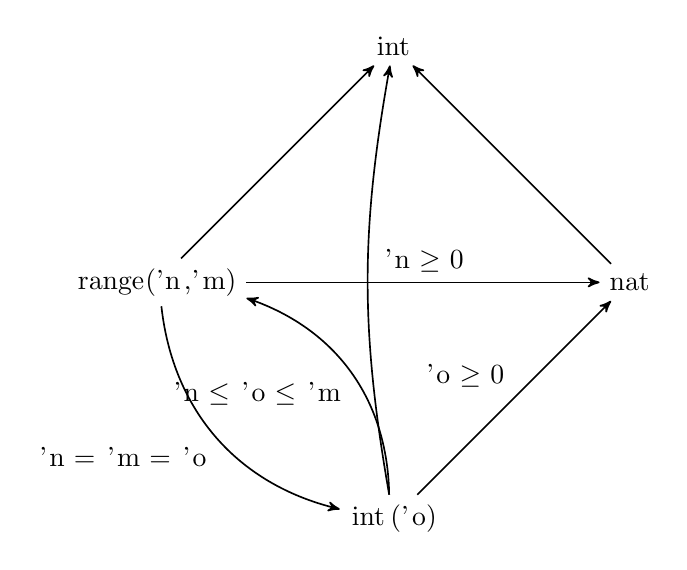
\begin{tikzpicture}
  [type/.style={rectangle},auto,>=stealth',semithick]
  \node[type] (int) at (0, 3) {\ll{int}};
  \node[type] (nat) at (3, 0) {\ll{nat}};
  \node[type] (range) at (-3, 0) {\ll{range('n,'m)}};
  \node[type] (atom) at (0, -3) {\ll{int('o)}};

  \draw[->] (nat) -- (int);
  \draw[->] (range) -- (int);
  \draw[->] (atom) to [bend left=10] node {} (int);
  \draw[->] (range) to node {\ll{'n} $\ge$ \ll{0}} (nat);
  \draw[->] (atom) to node {\ll{'o} $\ge$ \ll{0}} (nat);
  \draw[->] (atom) to [bend right=35] node {\ll{'n} $\le$ \ll{'o} $\le$ \ll{'m}} (range);
  \draw[->] (range) to [bend right=35] node [swap] {\ll{'n} $=$ \ll{'m} $=$ \ll{'o}} (atom);
\end{tikzpicture}
\end{center}

Note that \ll{bit} isn't a numeric type (i.e. it's not
\ll{range(0,1)}. This is intentional, as otherwise it would be
possible to write expressions like \ll{(1 : bit) + 5} which would end
up being equal to \ll{6 : range(5, 6)}. This kind of implicit casting
from bits to other numeric types would be highly undesirable. The
\ll{bit} type itself is a two-element type with members \ll{bitzero} and
\ll{bitone}.

\subsection{Vector Type}
\label{sec:vec}

Sail has the built-in type \ll{vector}, which is a polymorphic type for
fixed-length vectors. For example, we could define a vector \ll{v} of
three integers as follows:
\begin{lstlisting}
let v : vector(3, dec, int) = [1, 2, 3]
\end{lstlisting}
The first argument of the vector type is a numeric expression
representing the length of the vector, and the last is the type of the
vector's elements. But what is the second argument? Sail allows two
different types of vector orderings---increasing (\ll{inc}) and
decreasing (\ll{dec}). These two orderings are shown for the bitvector
0b10110000 below.

\begin{center}
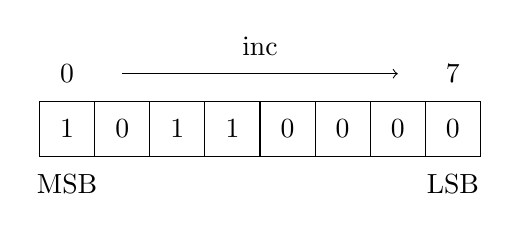
\begin{tikzpicture}[scale=0.7]
  \draw (0,0) rectangle (1,1) node[pos=.5] {1};
  \draw (1,0) rectangle (2,1) node[pos=.5] {0};
  \draw (2,0) rectangle (3,1) node[pos=.5] {1};
  \draw (3,0) rectangle (4,1) node[pos=.5] {1};
  \draw (4,0) rectangle (5,1) node[pos=.5] {0};
  \draw (5,0) rectangle (6,1) node[pos=.5] {0};
  \draw (6,0) rectangle (7,1) node[pos=.5] {0};
  \draw (7,0) rectangle (8,1) node[pos=.5] {0};

  \node at (.5,1.5) {0};
  \node at (7.5,1.5) {7};
  \draw[->] (1.5,1.5) -- (6.5,1.5);
  \node at (.5,-0.5) {MSB};
  \node at (7.5,-0.5) {LSB};
  \node at (4,2) {\ll{inc}};
\end{tikzpicture}
\qquad
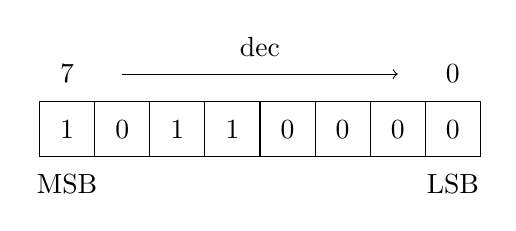
\begin{tikzpicture}[scale=0.7]
  \draw (0,0) rectangle (1,1) node[pos=.5] {1};
  \draw (1,0) rectangle (2,1) node[pos=.5] {0};
  \draw (2,0) rectangle (3,1) node[pos=.5] {1};
  \draw (3,0) rectangle (4,1) node[pos=.5] {1};
  \draw (4,0) rectangle (5,1) node[pos=.5] {0};
  \draw (5,0) rectangle (6,1) node[pos=.5] {0};
  \draw (6,0) rectangle (7,1) node[pos=.5] {0};
  \draw (7,0) rectangle (8,1) node[pos=.5] {0};

  \node at (.5,1.5) {7};
  \node at (7.5,1.5) {0};
  \draw[->] (1.5,1.5) -- (6.5,1.5);
  \node at (.5,-0.5) {MSB};
  \node at (7.5,-0.5) {LSB};
  \node at (4,2) {\ll{dec}};
\end{tikzpicture}
\end{center}

For increasing (bit)vectors, the 0 index is the most significant bit
and the indexing increases towards the least significant bit. Whereas
for decreasing (bit)vectors the least significant bit is 0 indexed,
and the indexing decreases from the most significant to the least
significant bit. For this reason, increasing indexing is sometimes
called `most significant bit is zero' or MSB0, while decreasing
indexing is sometimes called `least significant bit is zero' or
LSB0. While this vector ordering makes most sense for bitvectors (it
is usually called bit-ordering), in Sail it applies to all
vectors. A default ordering can be set using
\begin{lstlisting}
default Order dec
\end{lstlisting}
and this should usually be done right at the beginning of a
specification. Most architectures stick to either convention or the
other, but Sail also allows functions which are polymorphic over
vector order, like so:
\begin{lstlisting}
val foo : forall ('a : Order). vector(8, 'a, bit) -> vector(8, 'a, bit)
\end{lstlisting}

\paragraph{Bitvector Literals}

Bitvector literals in Sail are written as either
\lstinline[mathescape]{0x$\textit{hex string}$} or
\lstinline[mathescape]{0b$\textit{binary string}$}, for example
\ll{0x12FE} or \ll{0b1010100}. The length of a hex literal is always
four times the number of digits, and the length of binary string is
always the exact number of digits, so \ll{0x12FE} has length 16, while
\ll{0b1010100} has length 7.

\paragraph{Accessing and Updating Vectors}

A vector can be indexed by using the
\lstinline[mathescape]{$\textit{vector}$[$\textit{index}$]}
notation. So, in the following code:
\begin{lstlisting}
  let v : vector(4, dec, int) = [1, 2, 3, 4]
  let a = v[0]
  let b = v[3]
\end{lstlisting}
\ll{a} will be \ll{4}, and \ll{b} will be \ll{1} (note that \ll{v} is
\ll{dec}). By default, Sail will statically check for out of bounds
errors, and will raise a type error if it cannot prove that all such
vector accesses are valid.

Vectors can be sliced using the
%
\lstinline[mathescape]{$\textit{vector}$[$\textit{index}_{msb}$ .. $\textit{index}_{lsb}$]}
%
notation. The indexes are always supplied with the index closest to
the MSB being given first, so we would take the bottom 32-bits of a
decreasing bitvector \ll{v} as \ll{v[31 .. 0]}, and the upper 32-bits
of an increasing bitvector as \ll{v[0 .. 31]}, i.e. the indexing order
for decreasing vectors decreases, and the indexing order for
increasing vectors increases.

A vector index can be updated using
\lstinline[mathescape]{[$\textit{vector}$ with $\textit{index}$ = $\textit{expression}$]}
notation.
%
Similarly, a sub-range of a vector can be updated using
%
\lstinline[mathescape]{[$\textit{vector}$ with $\textit{index}_{msb}$ .. $\textit{index}_{lsb}$ = $\textit{expression}$]},
%
where the order of the indexes is the same as described above for
increasing and decreasing vectors.

These expressions are actually just syntactic sugar for several
built-in functions, namely \ll{vector_access}, \ll{vector_subrange},
\ll{vector_update}, and \ll{vector_update_subrange}.

\subsection{List Type}

In addition to vectors, Sail also has \ll{list} as a built-in type. For
example:
\begin{lstlisting}
let l : list(int) = [|1, 2, 3|]
\end{lstlisting}
The cons operator is \ll{::}, so we could equally write:
\lstinputlisting{examples/list.sail}
Pattern matching can be used to destructure lists, see Section~\ref{sec:pat}.

\subsection{Other Types}

Sail also has a \ll{string} type, and a \ll{real} type. The \ll{real}
type is used to model arbitrary real numbers, so floating point
instructions could be specified by mapping the floating point inputs
to real numbers, performing the arithmetic operation on the real
numbers, and then mapping back to a floating point value of the
appropriate precision.

\subsection{Pattern Matching}
\label{sec:pat}

Like most functional languages, Sail supports pattern matching via the
\ll{match} keyword. For example:
\begin{lstlisting}
let n : int = f();
match n {
  1 => print("1"),
  2 => print("2"),
  3 => print("3"),
  _ => print("wildcard")
}
\end{lstlisting}
The \ll{match} keyword takes an expression and then branches using a
pattern based on its value. Each case in the match expression takes
the form \lstinline[mathescape]{$\textit{pattern}$ => $\textit{expression}$},
separated by commas. The cases are checked sequentially from top to
bottom, and when the first pattern matches its expression will be
evaluated.

\ll{match} in Sail is not currently checked for exhaustiveness---after
all we could have arbitrary constraints on a numeric variable being
matched upon, which would restrict the possible cases in ways that we
could not determine with just a simple syntactic check. However, there
is a simple exhaustiveness checker which runs and gives warnings (not
errors) if it cannot tell that the pattern match is exhaustive, but
this check can give false positives. It can be turned off with the
\verb+-no_warn+ flag.

When we match on numeric literals, the type of the variable we are
matching on will be adjusted. In the above example in the
\ll{print("1")} case, $n$ will have the type \ll{int('e)}, where
\ll{'e} is some fresh type variable, and there will be a constraint
that \ll{'e} is equal to one.

We can also have guards on patterns, for example we could modify the
above code to have an additional guarded case like so:
\begin{lstlisting}
let n : int = f();
match n {
  1 => print("1"),
  2 => print("2"),
  3 => print("3"),
  m if m <= 10 => print("n is less than or equal to 10"),
  _ => print("wildcard")
}
\end{lstlisting}
The variable pattern m will match against anything, and the guard can
refer to variables bound by the pattern.

\paragraph{Matching on enums}

Match can be used to match on possible values of an enum, like so:
\begin{lstlisting}
enum E = A | B | C

match x {
  A => print("A"),
  B => print("B"),
  C => print("C")
}
\end{lstlisting}
Note that because Sail places no restrictions on the lexical structure
of enumeration elements to differentiate them from ordinary
identifiers, pattern matches on variables and enum elements can be
somewhat ambiguous. This is the primary reason why we have the basic,
but incomplete, pattern exhaustiveness check mentioned above---it can
warn you if removing an enum constructor breaks a pattern match.

\paragraph{Matching on tuples}

We use match to destructure tuple types, for example:
\begin{lstlisting}
let x : (int, int) = (2, 3) in
match x {
  (y, z) => print("y = 2 and z = 3")
}

\end{lstlisting}

\paragraph{Matching on unions}

Match can also be used to destructure union constructors, for example
using the option type from Section~\ref{sec:union}:
\begin{lstlisting}
match option {
  Some(x) => foo(x),
  None()  => print("matched None()")
}
\end{lstlisting}
Note that like how calling a function with a unit argument can be done
as \ll{f()} rather than \ll{f(())}, matching on a constructor \ll{C}
with a unit type can be achieved by using \ll{C()} rather than
\ll{C(())}.

\paragraph{Matching on bit vectors}

Sail allows numerous ways to match on bitvectors, for example:
\begin{lstlisting}
match v {
  0xFF => print("hex match"),
  0b0000_0001 => print("binary match"),
  0xF @ v : bits(4) => print("vector concatenation pattern"),
  0xF @ [bitone, _, b1, b0] => print("vector pattern"),
  _ : bits(4) @ v : bits(4) => print("annotated wildcard pattern")
}
\end{lstlisting}
We can match on bitvector literals in either hex or binary forms. We
also have vector concatenation patterns, of the form
\lstinline[mathescape]{$\mathit{pattern}$ @ $\ldots$ @ $\mathit{pattern}$}.
We must be able to infer the length of all the sub-patterns in a vector
concatenation pattern, hence why in the example above all the
wildcard and variable patterns beneath vector concatenation patterns
have type annotations. In the context of a pattern the \ll{:} operator
binds tighter than the \ll{@} operator (as it does elsewhere).

We also have vector patterns, which for bitvectors match on individual
bits. In the above example, \ll{b0} and \ll{b1} will have type
\ll{bit}. The pattern \ll{bitone} is a bit literal, with \ll{bitzero}
being the other bit literal pattern.

Note that because vectors in Sail are type-polymorphic, we can also
use both vector concatenation patterns and vector patterns to match
against non-bit vectors.

\paragraph{Matching on lists}

Sail allows lists to be destructured using patterns. There are two
types of patterns for lists, cons patterns and list literal patterns.

\begin{lstlisting}
match ys {
  x :: xs => print("cons pattern"),
  [||]    => print("empty list")
}
\end{lstlisting}

\begin{lstlisting}
match ys {
  [|1, 2, 3|] => print("list pattern"),
  _           => print("wildcard")
}
\end{lstlisting}

\paragraph{Matching on strings}

Unusually, Sail allows strings and concatenations of strings to be
used in pattern-matching. The match operates in a simple left-to-right
fashion.

\begin{lstlisting}
  match s {
    "hello" ^ " " ^ "world" => print("matched hello world"),
    _ => print("wildcard")
  }
\end{lstlisting}

Note that a string match is always greedy, so

\begin{lstlisting}
  match s {
    "hello" ^ s ^ "world" => print("matched hello" ^ s ^ "world"),
    "hello" ^ s => print("matched hello" ^ s),
    _ => print("wildcard")
  }
\end{lstlisting}

while syntactically valid, will never match the first case.

String matching is most often used with \emph{mappings}, covered
above, to allow parsing of strings containing, for example, integers:

\begin{lstlisting}
  match s {
    "int=" ^ int(x) ^ ";" => x
    _ => -1
  }
\end{lstlisting}

This is intended to be used to parse assembly languages.


\paragraph{As patterns}

Like OCaml, Sail also supports naming parts of patterns using the
\ll{as} keyword. For example, in the above list pattern we could bind
the entire list as zs as follows:
\begin{lstlisting}
match ys {
  x :: xs as zs => print("cons with as pattern"),
  [||]          => print("empty list")
}
\end{lstlisting}
The as pattern has lower precedence than any other keyword or operator
in a pattern, so in this example zs will refer to \ll{x :: xs}.

\subsection{Mutable and Immutable Variables}

Local immutable bindings can be introduced via the \ll{let} keyword,
which has the following form
\begin{center}
  \ll{let} \textit{pattern} \ll{=} \textit{expression} \ll{in} \textit{expression}
\end{center}
The pattern is matched against the first expression, binding any
identifiers in that pattern. The pattern can have any form, as in the
branches of a match statement, but it should be complete (i.e. it
should not fail to match)\footnote{although this is not checked right
  now}.

When used in a block, we allow a variant of the let statement, where
it can be terminated by a semicolon rather than the in keyword.
\begin{lstlisting}[mathescape]
{
  let $\textit{pattern}$ = $\textit{expression}_0$;
  $\textit{expression}_1$;
  $\vdots$
  $\textit{expression}_n$
}
\end{lstlisting}
This is equivalent to the following
\begin{lstlisting}[mathescape]
{
  let $\textit{pattern}$ = $\textit{expression}_0$ in {
    $\textit{expression}_1$;
    $\vdots$
    $\textit{expression}_n$
  }
}
\end{lstlisting}
If we were to write
\begin{lstlisting}[mathescape]
{
  let $\textit{pattern}$ = $\textit{expression}_0$ in
  $\textit{expression}_1$;
  $\vdots$
  $\textit{expression}_n$ // pattern not visible
}
\end{lstlisting}
instead, then \textit{pattern} would only be bound within
$\textit{expression}_1$ and not any further expressions. In general
the block-form of let statements terminated with a semicolon should
always be preferred within blocks.

Variables bound within function arguments, match statement, and
let-bindings are always immutable, but Sail also allows mutable
variables. Mutable variables are bound implicitly by using the
assignment operator within a block.
\begin{lstlisting}
{
  x : int = 3 // Create a new mutable variable x initialised to 3
  x = 2       // Rebind it to the value 2
}
\end{lstlisting}
The assignment operator is the equality symbol, as in C and other
programming languages. Sail supports a rich language of \emph{l-value}
forms, which can appear on the left of an assignment. These will be
described in Subsection~\ref{sec:lexp}. Note that we could have
written
\begin{lstlisting}
{
  x = 3;
  x = 2
}
\end{lstlisting}
but it would not have type-checked. The reason for this is if a
mutable variable is declared without a type, Sail will try to infer
the most specific type from the right hand side of the
expression. However, in this case Sail will infer the type as
\ll{int(3)} and will therefore complain when we try to reassign it to
\ll{2}, as the type \ll{int(2)} is not a subtype of \ll{int(3)}. We
therefore declare it as an \ll{int} which as mentioned in
Section~\ref{sec:numeric} is a supertype of all numeric types. Sail
will not allow us to change the type of a variable once it has been
created with a specific type. We could have a more specific type for
the variable \ll{x}, so
\begin{lstlisting}
{
  x : {|2, 3|} = 3;
  x = 2
}
\end{lstlisting}
would allow \ll{x} to be either 2 or 3, but not any other value. The
\lstinline+{|2, 3|}+ syntax is equivalent to \lstinline+{'n, 'n in {2, 3}. int('n)}+.

\subsubsection{Assignment and l-values}
\label{sec:lexp}

It is common in ISA specifications to assign to complex l-values,
e.g.~to a subvector or named field of a bitvector register, or to an
l-value computed with some auxiliary function, e.g.~to select the
appropriate register for the current execution model.

We have l-values that allow us to write to individual elements of a
vector:
\begin{lstlisting}
{
  v : bits(8) = 0xFF;
  v[0] = bitzero;
  assert(v == 0xFE)
}
\end{lstlisting}
as well as sub ranges of a vector:
\begin{lstlisting}
{
  v : bits(8) = 0xFF;
  v[3 .. 0] = 0x0; // assume default Order dec
  assert(v == 0xF0)
}
\end{lstlisting}
We also have vector concatenation l-values, which work much like
vector concatenation patterns
\begin{lstlisting}
{
  v1 : bits(4) = 0xF;
  v2 : bits(4) = 0xF;
  v1 @ v2 = 0xAB;
  assert(v1 == 0xA & v2 == 0xB)
}
\end{lstlisting}
For structs we can write to an individual struct field as
\begin{lstlisting}
{
  s : S = struct { field = 0xFF }
  s.field = 0x00
}
\end{lstlisting}
assume we have a struct type \ll{S}, with a field simply called
\ll{field}. We can do multiple assignment using tuples, e.g.
\begin{lstlisting}
{
  (x, y) = (2, 3);
  assert(x == 2 & x == 3)
}
\end{lstlisting}

Finally, we allow functions to appear in l-values. This is a very
simple way to declare `setter' functions that look like custom
l-values, for example:
\begin{lstlisting}
{
  memory(addr) = 0x0F
}
\end{lstlisting}
This works because \ll{f(x) = y} is sugar for \ll{f(x, y)}. This
feature is commonly used when setting registers or memory that has
additional semantics for when they are read or written. We commonly
use the overloading feature to declare what appear to be getter/setter
pairs, so the above example we could implement a \ll{read_memory}
function and a \ll{write_memory} function and overload them both as
\ll{memory} to allow us to write memory using \ll{memory(addr) = data}
and read memory as \ll{data = memory(addr)}, as so:
\begin{lstlisting}
val read_memory : bits(64) -> bits(8)
val write_memory : (bits(64), bits(8)) -> unit

overload memory = {read_memory, write_memory}
\end{lstlisting}
For more details on operator and function overloading see
Section~\ref{sec:overload}.

\subsection{Registers}

Registers can be declared with a top level
\begin{center}
  \ll{register} \textit{name} \ll{:} \textit{type}
\end{center}
declaration. Registers are essentially top-level global variables and
can be set with the previously discussed l-expression forms. There is
currently no restriction on the type of a register in
Sail.\footnote{We may at some point want to enforce that they can be
  mapped to bitvectors.}

Registers differ from ordinary mutable variables as we can pass around
references to them by name. A reference to a register \ll{R} is
created as \ll{ref R}. If the register \ll{R} has the type \ll{A},
then the type of \ll{ref R} will be \ll{register(A)}. There is a
dereferencing l-value operator \ll{*} for assigning to a register
reference. One use for register references is to create a list of
general purpose registers, so they can be indexed using numeric
variables. For example:
\lstinputlisting{examples/regref.sail}

We can dereference register references using the \ll{"reg_deref"}
builtin (see Section~\ref{sec:prelude}), which is set up like so:
\begin{lstlisting}
val "reg_deref" : forall ('a : Type). register('a) -> 'a effect {rreg}
\end{lstlisting}
Currently there is no built-in syntactic sugar for dereferencing
registers in expressions.

Unlike previous versions of Sail, referencing and de-referencing
registers is done explicitly, although we can use an automatic cast to
implicitly dereference registers if that semantics is desired for a
specific specification that makes heavy use of register references,
like so:
\begin{lstlisting}
val cast auto_reg_deref = "reg_deref" : forall ('a : Type). register('a) -> 'a effect {rreg}
\end{lstlisting}


\subsection{Type declarations}

\subsubsection{Enumerations}

Enumerations can be defined in either a Haskell-like syntax (useful
for smaller enums) or a more traditional C-like syntax, which is often
more readable for enumerations with more members. There are no lexical
constraints on the identifiers that can be part of an
enumeration. There are also no restrictions on the name of a
enumeration type, other than it must be a valid identifier. For
example, the following shows two ways to define the enumeration
\ll{Foo} with three members, \ll{Bar}, \ll{Baz}, and \ll{quux}:

\lstinputlisting{examples/enum1.sail}
\lstinputlisting{examples/enum2.sail}

For every enumeration type $E$ sail generates a
\lstinline[mathescape]{num_of_$E$} function and a
\lstinline[mathescape]{$E$_of_num} function, which for \ll{Foo} above
will have the following definitions\footnote{It will ensure that the
  generated function name \ll{arg} does not clash with any enumeration
  constructor.}:
\begin{lstlisting}
val Foo_of_num : forall 'e, 0 <= 'e <= 2. int('e) -> Foo
function Foo_of_num(arg) = match arg {
  0 => Bar,
  1 => Baz,
  _ => quux
}

val num_of_Foo : Foo -> {'e, 0 <= 'e <= 2. int('e)}
function num_of_Foo(arg) = match arg {
  Bar  => 0,
  Baz  => 1,
  quux => 2
}
\end{lstlisting}
Note that these functions are not automatically made into implicit
casts.

\subsubsection{Structs}

Structs are defined using the struct keyword like so:
\lstinputlisting{examples/struct.sail}

If we have a struct \ll{foo : Foo}, its fields can be accessed by
\ll{foo.bar}, and set as \ll{foo.bar = 0xF}. It can also be updated in
a purely functional fashion using the construct \ll{\{foo with bar =
  0xF\}}. A new struct value can be created with
\ll{struct \{foo = 0xF, baz = 42, quux = 3\}}. There is no lexical
restriction on the name of a struct or the names of its fields.
Pattern matching on structs is not possible.

\subsubsection{Unions}
\label{sec:union}

As an example, the \ll{maybe} type \`{a} la Haskell could be defined
in Sail as follows:
\begin{lstlisting}
union maybe ('a : Type) = {
  Just : 'a,
  None : unit
}
\end{lstlisting}
Constructors, such as \ll{Just} are called like functions, as in
\ll{Just(3) : maybe(int)}. The \ll{None} constructor is also called in
this way, as \ll{None()}. Notice that unlike in other languages, every
constructor must be associated with a type---there are no nullary
constructors. As with structs there are no lexical restrictions on the
names of either the constructors nor the type itself, other than they
must be valid identifiers.

\subsubsection{Bitfields}
\label{sec:bitfield}

The following example creates a bitfield type called \ll{cr} and a
register \ll{CR} of that type.

\lstinputlisting{examples/bitfield.sail}

A bitfield definition creates a wrapper around a bit vector type, and
generates getters and setters for the fields. For the setters, it is
assumed that they are being used to set registers with the bitfield
type\footnote{This functionality was originally called \emph{register
    types} for this reason, but this was confusing because types of
  registers are not always register types.}. If the bitvector is
decreasing then indexes for the fields must also be in decreasing
order, and vice-versa for an increasing vector. For the above example,
the bitfield wrapper type will be the following:

\begin{lstlisting}
struct cr = {bits : bitvector(8, dec)}
\end{lstlisting}

The complete vector can be accessed as \ll{CR.bits()}, and a register
of type \ll{cr} can be set like \ll{CR->bits() = 0xFF}. Getting and
setting individual fields can be done similarly, as \ll{CR.CR0()} and
\ll{CR->CR0() = 0xF}. Internally, the bitfield definition will
generate a \lstinline[mathescape]{_get_$F$} and
\lstinline[mathescape]{_set_$F$} function for each field
\lstinline[mathescape]{$F$}, and then overload them as
\lstinline[mathescape]{_mod_$F$} for the accessor syntax. The setter
takes the bitfield as a reference to a register, hence why we use the
\ll{->} notation. For pure updates of values of type \ll{cr} a
function \lstinline[mathescape]{update_$F$} is also defined. For more
details on getters and setters, see Section~\ref{sec:lexp}. A
singleton bit in a bitfield definition, such as \ll{LT : 7} will be
defined as a bitvector of length one, and not as a value of type
\ll{bit}, which mirrors the behaviour of ARM's ASL language.

\subsection{Operators}

Valid operators in Sail are sequences of the following non
alpha-numeric characters: \verb#!%&*+-./:<>=@^|#. Additionally, any
such sequence may be suffixed by an underscore followed by any valid
identifier, so \verb#<=_u# or even \verb#<=_unsigned# are valid
operator names. Operators may be left, right, or non-associative, and
there are 10 different precedence levels, ranging from 0 to 9, with 9
binding the tightest. To declare the precedence of an operator, we use a fixity declaration like:
\begin{lstlisting}
infix 4 <=_u
\end{lstlisting}
For left or right associative operators, we'd use the keywords
\ll{infixl} or \ll{infixr} respectively. An operator can be used
anywhere a normal identifier could be used via the \ll{operator}
keyword. As such, the \verb#<=_u# operator can be defined as:
\begin{lstlisting}
val operator <=_u : forall 'n. (bits('n), bits('n)) -> bool
function operator <=_u(x, y) = unsigned(x) <= unsigned(y)
\end{lstlisting}

\paragraph{Builtin precedences}
The precedence of several common operators are built into Sail. These
include all the operators that are used in type-level numeric
expressions, as well as several common operations such as equality,
division, and modulus. The precedences for these operators are
summarised in Table~\ref{tbl:operators}.

\begin{table}[hbt]
  \center
  \begin{tabular}{| c || l | l | l |}
    \hline
    Precedence & Left associative & Non-associative & Right associative\\
    \hline
    9 & & &\\
    \hline
    8 & & & \ll{^}\\
    \hline
    7 & \ll{*}, \ll{/}, \ll{\%} & &\\
    \hline
    6 & \ll{+}, \ll{-} & &\\
    \hline
    5 & & &\\
    \hline
    4 & & \ll{<}, \ll{<=}, \ll{>}, \ll{>=}, \ll{!=}, \ll{=}, \ll{==} &\\
    \hline
    3 & & & \ll{&}\\
    \hline
    2 & & & \ll{|}\\
    \hline
    1 & & &\\
    \hline
    0 & & &\\
    \hline
  \end{tabular}
  \caption{Default Sail operator precedences}
  \label{tbl:operators}
\end{table}

\paragraph{Type operators}
Sail allows operators to be used at the type level. For example, we
could define a synonym for the built-in \ll{range} type as:
\lstinputlisting{examples/type_operator.sail} Note that we can't use
\ll{..} as an operator name, because that is reserved syntax for
vector slicing. Operators used in types always share precedence with
identically named operators at the expression level.

\subsection{Ad-hoc Overloading}
\label{sec:overload}

Sail has a flexible overloading mechanism using the \ll{overload}
keyword
\begin{center}
  \ll{overload} \textit{name} \ll{=} \lstinline+{+ \textit{name}$_1$ \ll{,} \ldots \ll{,} \textit{name}$_n$ \lstinline+}+
\end{center}
This takes an identifier name, and a list of other identifier names to
overload that name with. When the overloaded name is seen in a Sail
definition, the type-checker will try each of the overloads in order
from left to right (i.e. from $\textit{name}_1$ to $\textit{name}_n$).
until it finds one that causes the resulting expression to type-check
correctly.

Multiple \ll{overload} declarations are permitted for the same
identifier, with each overload declaration after the first adding its
list of identifier names to the right of the overload list (so earlier
overload declarations take precedence over later ones). As such, we
could split every identifier from above syntax example into its own
line like so:
\begin{center}
  \ll{overload} \textit{name} \ll{=} \lstinline+{+ \textit{name}$_1$ \lstinline+}+\\
  $\vdots$\\
  \ll{overload} \textit{name} \ll{=} \lstinline+{+ \textit{name}$_n$ \lstinline+}+
\end{center}

As an example for how overloaded functions can be used, consider the
following example, where we define a function \ll{print_int} and a
function \ll{print_string} for printing integers and strings
respectively. We overload \ll{print} as either \ll{print_int} or
\ll{print_string}, so we can print either number such as 4, or strings
like \ll{"Hello, World!"} in the following \ll{main} function
definition.

\lstinputlisting{examples/overload.sail}

We can see that the overloading has had the desired effect by dumping
the type-checked AST to stdout using the following command
\verb+sail -ddump_tc_ast examples/overload.sail+. This will print the
following, which shows how the overloading has been resolved
\begin{lstlisting}
function main () : unit = {
  print_string("Hello, World!");
  print_int(4)
}
\end{lstlisting}
This option can be quite useful for testing how overloading has been
resolved. Since the overloadings are done in the order they are listed
in the source file, it can be important to ensure that this order is
correct. A common idiom in the standard library is to have versions of
functions that guarantee more constraints about their output be
overloaded with functions that accept more inputs but guarantee less
about their results. For example, we might have two division functions:
\begin{lstlisting}
val div1 : forall 'm 'n, 'n >= 0 & 'm > 0. (int('n), int('m)) -> {'o, 'o >= 0. int('o)}

val div2 : (int, int) -> option(int)
\end{lstlisting}
The first guarantees that if the first argument is greater than or
equal to zero, and the second argument is greater than zero, then the
result will be greater than or equal to zero. If we overload these
definitions as
\begin{lstlisting}
overload operator / = {div1, div2}
\end{lstlisting}
Then the first will be applied when the constraints on its inputs can
be resolved, and therefore the guarantees on its output can be
guaranteed, but the second will be used when this is not the case, and
indeed, we will need to manually check for the division by zero case
due to the option type. Note that the return type can be very
different between different cases in the overload.

The amount of arguments overloaded functions can have can also vary,
so we can use this to define functions with optional arguments, e.g.
\lstinputlisting{examples/zeros.sail} In this example, we can call
\ll{zero_extend} and the return length is implicit (likely using
\ll{sizeof}, see Section~\ref{sec:sizeof}) or we can provide it
ourselves as an explicit argument.

%% \subsection{Getters and Setters}
%% \label{sec:getset}

%% We have already seen some examples of getters and setters in
%% Subsection~\ref{sec:bitfield}, but they can be used in many other
%% contexts.

%% \fbox{TODO}

\subsection{Sizeof and Constraint}
\label{sec:sizeof}

As already mentioned in Section~\ref{sec:functions}, Sail allows for
arbitrary type variables to be included within expressions. However,
we can go slightly further than this, and include both arbitrary
(type-level) numeric expressions in code, as well as type
constraints. For example, if we have a function that takes two
bitvectors as arguments, then there are several ways we could compute
the sum of their lengths.
\begin{lstlisting}
val f : forall 'n 'm. (bits('n), bits('m)) -> unit

function f(xs, ys) = {
  let len = length(xs) + length(ys);
  let len = 'n + 'm;
  let len = sizeof('n + 'm);
  ()
}
\end{lstlisting}
Note that the second line is equivalent to
\begin{lstlisting}
  let len = sizeof('n) + sizeof('n)
\end{lstlisting}

There is also the \ll{constraint} keyword, which takes a type-level constraint and allows it to be used as a boolean expression, so we could write:
\begin{lstlisting}
function f(xs, ys) = {
  if constraint('n <= 'm) {
    // Do something
  }
}
\end{lstlisting}
rather than the equivalent test \ll{length(xs) <= length(ys)}. This way
of writing expressions can be succinct, and can also make it very
explicit what constraints will be generated during flow
typing. However, all the constraint and sizeof definitions must be
re-written to produce executable code, which can result in the
generated theorem prover output diverging (in appearance) somewhat
from the source input. In general, it is probably best to use
\ll{sizeof} and \ll{constraint} sparingly.

However, as previously mentioned both \ll{sizeof} and \ll{constraint}
can refer to type variables that only appear in the output or are
otherwise not accessible at runtime, and so can be used to implement
implicit arguments, as was seen for \ll{replicate_bits} in
Section~\ref{sec:functions}.

\subsection{Scattered Definitions}
\label{sec:scattered}
In a Sail specification, sometimes it is desirable to collect together
the definitions relating to each machine instruction (or group
thereof), e.g.~grouping the clauses of an AST type with the associated
clauses of decode and execute functions, as in
Section~\ref{sec:riscv}. Sail permits this with syntactic sugar for
`scattered' definitions. Either functions or union types can be
scattered.

One begins a scattered definition by declaring the name and kind
(either function or union) of the scattered definition, e.g.
\begin{lstlisting}
scattered function foo

scattered union bar
\end{lstlisting}
This is then followed by a list of clauses for either the union or the
function, which can be freely interleaved with other definitions (such
as \ll{E} in the below code)
\begin{lstlisting}[mathescape]
union clause bar : Baz(int, int)

function clause foo(Baz(x, y)) = $\ldots$

enum E = A | B | C

union clause bar : Quux(string)

function clause foo(Quux(str)) = print(str)
\end{lstlisting}
Finally the scattered definition is ended with the \ll{end} keyword, like so:
\begin{lstlisting}
end foo

end bar
\end{lstlisting}

Semantically, scattered definitions of union types appear at the start
of their definition, and scattered definitions of functions appear at
the end. A scattered function definition can be recursive, but
mutually recursive scattered function definitions should be avoided.

\subsection{Exceptions}
\label{sec:exn}

Perhaps surprisingly for a specification language, Sail has exception
support. This is because exceptions as a language feature do sometimes
appear in vendor ISA pseudocode, and such code would be very difficult
to translate into Sail if Sail did not itself support exceptions. We
already translate Sail to monadic theorem prover code, so working with
a monad that supports exceptions there is fairly natural.

For exceptions we have two language features: \ll{throw} statements
and \ll{try}-\ll{catch} blocks. The throw keyword takes a value of
type \ll{exception} as an argument, which can be any user defined type
with that name. There is no builtin exception type, so to use
exceptions one must be set up on a per-project basis. Usually the
exception type will be a union, often a scattered union, which allows
for the exceptions to be declared throughout the specification as they
would be in OCaml, for example: \lstinputlisting{examples/exn.sail}
Note how the use of the scattered type allows additional exceptions to
be declared even after they are used.

\subsection{Preludes and Default Environment}
\label{sec:prelude}

By default Sail has almost no built-in types or functions, except for
the primitive types described in this Chapter. This is because
different vendor-pseudocodes have varying naming conventions and
styles for even the most basic operators, so we aim to provide
flexibility and avoid committing to any particular naming convention or
set of built-ins. However, each Sail backend typically implements
specific external names, so for a PowerPC ISA description one might
have:
\begin{lstlisting}[mathescape]
val EXTZ = "zero_extend" : $\ldots$
\end{lstlisting}
while for ARM, one would have
\begin{lstlisting}[mathescape]
val ZeroExtend = "zero_extend" : $\ldots$
\end{lstlisting}
where each backend knows about the \ll{"zero_extend"} external name,
but the actual Sail functions are named appropriately for each
vendor's pseudocode. As such each Sail ISA spec tends to have its own
prelude.

However, the \verb+lib+ directory in the Sail repository contains some
files that can be included into any ISA specification for some basic
operations. These are listed below:
\begin{description}
  \item[flow.sail] Contains basic definitions required for flow
    typing to work correctly.
  \item[arith.sail] Contains simple arithmetic operations for
    integers.
  \item[vector\_dec.sail] Contains operations on decreasing
    (\ll{dec}) indexed vectors, see Section~\ref{sec:vec}.
  \item[vector\_inc.sail] Like \verb+vector_dec.sail+, except
    for increasing (\ll{inc}) indexed vectors.
  \item[option.sail] Contains the definition of the option
    type, and some related utility functions.
  \item[prelude.sail] Contains all the above files, and chooses
    between \verb+vector_dec.sail+ and \verb+vector_inc.sail+ based on
    the default order (which must be set before including this file).
  \item[smt.sail] Defines operators allowing div, mod, and abs
    to be used in types by exposing them to the Z3 SMT solver.
  \item[exception\_basic.sail] Defines a trivial exception type, for
    situations where you don't want to declare your own (see
    Section~\ref{sec:exn}).
\end{description}


\section{Type System}
\label{sec:types}

(This section is still a work in progress)

\newcommand{\tcheck}[3]{#1 \vdash #2 \Leftarrow #3}
\newcommand{\tinfer}[3]{#1 \vdash #2 \Rightarrow #3}
\newcommand{\msail}[1]{\text{\lstinline[mathescape]+#1+}}

\subsection{Blocks}
\label{subsec:blocks}

\[
\frac{\tcheck{\Gamma}{E_0}{\text{\lstinline+bool+}}
      \qquad
      \tcheck{\Gamma}{M}{\text{\lstinline+string+}}
      \qquad
      \tcheck{\mathrm{FlowThen}(\Gamma, E_0)}{\text{\lstinline[mathescape]+\{$E_1$; $\ldots$; $E_n$\}+}}{A}}
     {\tcheck{\Gamma}{\text{\lstinline[mathescape]+\{assert($E_0$, $M$); $E_1$; $\ldots$; $E_n$ \}+}}{A}}
\]

\[
\frac{\tcheck{\mathrm{BindAssignment}(\Gamma, L_0, E_0)}{\text{\lstinline[mathescape]+\{$E_1$; $\ldots$; $E_n$\}+}}{A}}
     {\tcheck{\Gamma}{\text{\lstinline[mathescape]+\{$L_0$ = $E_0$; $E_1$; $\ldots$; $E_n$ \}+}}{A}}
\]

\[
\frac{\tcheck{\Gamma}{E_0}{\text{\lstinline+unit+}}
      \qquad
      \tcheck{\Gamma}{\text{\lstinline[mathescape]+\{$E_1$; $\ldots$; $E_n$\}+}}{A}}
     {\tcheck{\Gamma}{\text{\lstinline[mathescape]+\{$E_0$; $E_1$; $\ldots$; $E_n$ \}+}}{A}}
\]

\[
\frac{\tcheck{\Gamma}{E}{A}}
     {\tcheck{\Gamma}{\text{\lstinline[mathescape]+\{$E$\}+}}{A}}
\]

\subsection{Let bindings}

Note that \lstinline[mathescape]+{let x = y; $E_0$; $\ldots$; $E_n$}+
is equivalent to \lstinline[mathescape]+{let x = y in {$E_0$; $\ldots$; $E_n$}}+,
which is why there are no special cases for let bindings in Subsection~\ref{subsec:blocks}.

\[
\frac{\tcheck{\Gamma}{E_0}{B}
      \qquad
      \tcheck{\mathrm{BindPattern}(\Gamma, P, B)}{E_1}{A}}
     {\tcheck{\Gamma}{\msail{let $\;P\;$ : $\;B\;$ = $\;E_0\;$ in $\;E_1$}}{A}}
\]

\[
\frac{\tinfer{\Gamma}{E_0}{B}
      \qquad
      \tcheck{\mathrm{BindPattern}(\Gamma, P, B)}{E_1}{A}}
     {\tcheck{\Gamma}{\msail{let $\;P\;$ = $\;E_0\;$ in $\;E_1$}}{A}}
\]

\paragraph{Pattern bindings} The $\mathrm{BindPattern}$ and $\mathrm{BindPattern}'$ functions are used to bind patterns into an environment. The first few cases are simple, if we bind an identifier $x$ against a type $T$, where $x$ is either immutable or unbound, then $x : T$ is added to the environment. If we bind a type against a wildcard pattern, then the environment is returned unchanged. An \lstinline+as+ pattern binds its variable with the appropriate type then recursively binds the rest of the pattern. When binding patterns we always bind against the base type, and bring existentials into scope, which is why $\mathrm{BindPattern}$ does this and then calls the $\mathrm{BindPattern}'$ function which implements all the cases.
\begin{align*}
  \mathrm{BindPattern}(\Gamma, P, T) &= \mathrm{BindPattern}'(\Gamma \lhd T, P, \mathrm{Base}(T))\\
  \mathrm{BindPattern}'(\Gamma, x, T) &= \Gamma \oplus x : T, \tag{$x$ is unbound or immutable}\\
  \mathrm{BindPattern}'(\Gamma, \msail{_}, T) &= \Gamma,\\
  \mathrm{BindPattern}'(\Gamma, \msail{$P\;$ as $\;x$}, T) &= \mathrm{BindPattern}(\Gamma \oplus x : T, P, T). \tag{$x$ is unbound or immutable}
\end{align*}
If we try to bind a numeric literal $n$ against a type
\lstinline[mathescape]+int($N$)+ then we add a constraint to the
environment that the nexp $N$ is equal to $n$.
\begin{align*}
\mathrm{BindPattern}'(\Gamma, n, \msail{int($N$)}) &= \Gamma \oplus (N = n).
\end{align*}
We also have some rules for typechecking lists, as well as user
defined constructors in unions (omitted here)
\begin{align*}
  \mathrm{BindPattern}'(\Gamma, [], \msail{list($A$)}) &= \Gamma,\\
  \mathrm{BindPattern}'(\Gamma, \msail{$P_{\mathit{hd}}\;$ :: $\;P_{\mathit{tl}}$}, \msail{list($A$)})
  &= \mathrm{BindPattern}(\mathrm{BindPattern}(\Gamma,P_{\mathit{hd}},A),P_{\mathit{tl}},\msail{list($A$)}).
\end{align*}

The pattern binding code follows a similar structure to the
bi-directional nature of the typechecking rules---the
$\mathrm{BindPattern}$ function acts like a checking rule where we
provide the type, and there is also an $\mathrm{InferPattern}$
function which acts like bind pattern but infers the types from the
patterns. There is therefore a final case
$\mathrm{BindPattern}(\Gamma, P, T) = \Gamma'$ where
$(\Gamma', T') = \mathrm{InferPattern}(\Gamma, P)$ and $T \subseteq T'$.

The $\mathrm{InferPattern}$ function is defined by the following cases
\begin{align*}
  \mathrm{InferPattern}(\Gamma,x) &= (\Gamma, T_{\mathit{enum}}), \tag{$x$ is an element of enumeration $T_{\mathit{enum}}$}\\
  \mathrm{InferPattern}(\Gamma,L) &= (\Gamma, \mathrm{InferLiteral}(L)), \tag{$L$ is a literal}\\
  \mathrm{InferPattern}(\Gamma,\msail{$P\;$ : $\;T$}) &= (\mathrm{BindPattern}(\Gamma,P,T), T).
\end{align*}

\paragraph{Type patterns} There is one additional case for $\mathrm{BindPattern}'$ which we haven't discussed. \TODO{type patterns}

\subsection{If statements}

\[
\frac{\tcheck{\Gamma}{E_{\mathit{if}}}{\msail{bool}}
      \qquad
      \tcheck{\mathrm{FlowThen}(\Gamma, E_{\mathit{if}})}{E_{\mathit{then}}}{A}
      \qquad
      \tcheck{\mathrm{FlowElse}(\Gamma, E_{\mathit{if}})}{E_{\mathit{else}}}{A}}
     {\tcheck{\Gamma}{\msail{if $\;E_{\mathit{if}}\;$ then $\;E_{\mathit{then}}\;$ else $\;E_{\mathit{else}}\;$}}{A}}
\]

\subsection{Return}

When checking the body of a function, the expected return type of the
function is placed into the context $\Gamma$.

\[
\frac{\tcheck{\Gamma}{E}{\mathrm{Return}(\Gamma)}}
     {\tcheck{\Gamma}{\msail{return($E$)}}{A}}
\]

\subsection{Functions}

Depending on the context, functions can be either checked or
inferred---although the only difference between the two cases is that
in the checking case we can use the expected return type to resolve
some of the function quantifiers, whereas in the inferring case we
cannot.

\begin{align*}
  \frac{
    f : \forall Q, C.(B_0,\ldots,B_n) \rightarrow R \in \Gamma
    \quad \textsc{InferFun}(\Gamma,Q,C,(B_0,\ldots,B_n),R,(x_0,\ldots,x_n)) = R'
  } {
    \tinfer{\Gamma}{f(x_0, \ldots, x_n)}{R'}
  }
\end{align*}

\begin{align*}
  \frac{
    f : \forall Q, C.(B_0,\ldots,B_n) \rightarrow R \in \Gamma
    \quad \textsc{CheckFun}(\Gamma,Q,C,(B_0,\ldots,B_n),R,(x_0,\ldots,x_n),R')
  } {
    \tcheck{\Gamma}{f(x_0, \ldots, x_n)}{R'}
  }
\end{align*}

The rules for checking or inferring functions are rather more
complicated than the other typing rules and are hard to describe in
purely logical terms, so they are instead presented as an algorithm in
Figure~\ref{fig:funapp}. Roughly the inference algorithm works as
follows:

\begin{enumerate}
\item \textsc{InferFun} takes as input the typing context $\Gamma$, the
  list of quantifiers $Q$ (a list of type variable/kind pairs), a
  constraint $C$, the function argument types $B_0\ldots B_n$, the
  function return type $R$, and finally this list of argument
  expressions the function is applied to $x_0\ldots x_n$.

\item We create an empty list of unsolved typing goals
  (expression/type pairs) called $\mathit{unsolved}$, a list of
  constraints $\mathit{Constraints}$, and a set of existential
  variables $\mathit{Existentials}$.

\item We iterate over each argument expression and type $x_m$ and
  $B_m$, if $x_m$ contains free type variables in $Q$ we infer the
  type of $x_n$ and attempt to unify that inferred type with $B_m$. If
  this unification step fails we add $(x_m, B_m)$ to the list of
  unsolved goals. This unification step may generate new existential
  variables and constraints which are added to $\mathit{Existentials}$
  and $\mathit{Constraints}$ as needed. The results of this
  unification step are used to resolve the universally-quantified type
  variables in $Q$. If $x_m$ does not contain free type variables in
  $Q$, then we simply check it against $B_m$.

\item After this loop has finished we expect all the type variables in
  $Q$ to have been resolved. If not, we throw a type error.

\item We now try to prove the function's constraint $C$ using the
  resolved type variables, and check any remaining function arguments
  in $\mathit{unsolved}$.

\item Finally, we add any new existentials and constraints to the
  function's return type $R$, simplifying if at all possible (using
  \textsc{SimplifyExist}), before returning this type as the inferred
  type of the function.
\end{enumerate}

\noindent The \textsc{CheckFun} calls the \textsc{InferFun} function, but it
takes an additional $X$ argument which the the required return type in
the context where the function being checked is called. It
additionally unifies the function's declared return type with the
expected return type, and uses this to resolve any quantifiers in $Q$,
provided that the return type is not existentially quantified. It may
also be required to coerce $R$ into $X$.

\begin{figure}[p]
\begin{algorithmic}[1]
  \Function{InferFun}{$\Gamma,Q, C, (B_0,\ldots,B_n), R, (x_0, \ldots, x_n)$}
  \State $\mathit{unsolved}\gets []$;
  $\mathit{Constraints}\gets []$;
  $\mathit{Existentials}\gets \emptyset$
  \ForAll{$m \in 0, \ldots, n$}
    \If{$B_m$ contains type variables in $Q$}
    \State $\Gamma \vdash x_m \Rightarrow E$
    \Comment Infer the type of $x_m$ as $E$
      \State $\mathit{unifiers}, \mathit{existentials}, \mathit{constraint} \gets$ \Call{CoerceAndUnify}{$\Gamma,E,B$}
      \If{\textsc{CoerceAndUnify} failed with \textsc{UnificationError}}
        \State $\mathit{unsolved}\gets (x_m,B_m) : \mathit{unsolved}$
        \State \textbf{continue}
        \Comment Skip to next iteration of loop
      \ElsIf{$\mathit{existentials}$ is not empty}
        \State Add type variables $\mathit{existentials}$ to $\Gamma$
        \State Add constraint $\mathit{constraint}$ to $\Gamma$
        \State $\mathit{Constraints}\gets \mathit{constraint} : \mathit{Constraints}$
        \State $\mathit{Existentials}\gets \mathit{existentials} \cup \mathit{Existentials}$
      \EndIf
      \ForAll{$(\mathit{nvar}, \mathit{nexp}) \in \mathit{unifiers}$}
        \State $B_0,...,B_n\gets B_0[\mathit{nvar} := \mathit{nexp}],\ldots,B_n[\mathit{nvar} := \mathit{nexp}]$
        \State $R\gets R[\mathit{nvar} := \mathit{nexp}]$;
        $C\gets C[\mathit{nvar} := \mathit{nexp}]$
        \State Remove $\mathit{nvar}$ from $Q$
      \EndFor
    \ElsIf{$B_m$ does not contain type variables in $Q$}
      \State $\tcheck{\Gamma}{x_m}{B_m}$
      \Comment Check type of $x_m$ against $B_m$
    \EndIf
  \EndFor
  \If{$Q$ is not empty}
    \State \textbf{raise} \textsc{TypeError}
    \Comment Unresolved universal quantifers
  \EndIf
  \State \Call{Prove}{$\Gamma, C$}
  \ForAll{$(x_m,B_m) \in \mathit{unsolved}$}
    $\tcheck{\Gamma}{x_m}{B_m}$
  \EndFor
  \State \Return \Call{SimplifyExist}{$\mathtt{exist}\ \mathit{Existentials}, \mathit{Constraints}.\ R$}
  \EndFunction\\

  \Function{CheckFun}{$\Gamma,Q,C,(B_0,\ldots,B_n),R,(x_0,\ldots,x_n),X$}
  \If{$X$ and $R$ are not existentially quantified}
    \State $\mathit{unifiers}, \_, \_ \gets$ \Call{Unify}{$\Gamma,R,X$}
    \If{\textsc{Unify} failed with \textsc{UnificationError}}
      \textbf{skip}
    \Else
      \ForAll{$(\mathit{nvar}, \mathit{nexp}) \in \mathit{unifiers}$}
        \State $B_0,...,B_n\gets B_0[\mathit{nvar} := \mathit{nexp}],\ldots,B_n[\mathit{nvar} := \mathit{nexp}]$
        \State $R\gets R[\mathit{nvar} := \mathit{nexp}]$;
        $C\gets C[\mathit{nvar} := \mathit{nexp}]$
        \State Remove $\mathit{nvar}$ from $Q$
      \EndFor
    \EndIf
  \EndIf
  \State $R'\gets$ \Call{InferFun}{$\Gamma,Q,C,(B_0,\ldots,B_n),R,(x_0,\ldots,x_n)$}
  \State \Return \Call{Coerce}{$R',X$}
  \EndFunction
\end{algorithmic}
\label{fig:funapp}
\caption{Inference and checking algorithms for function calls}
\end{figure}


\bibliographystyle{unsrt}
\bibliography{manual}

\end{document}
